%%%%%%%%%%%%%%%%%%%%%%%%%%%%%%%%%%%%%%%%%%%%%%%
%
% Template for Master degrees
% DISI - Department of Information Engineering and Computer Science
%
% update 2020-08-30
%
% To generate pdf 
% pdflatex __filename__.tex
% bibtex __file_name__.aux
% pdflatex __file_name__.tex
% pdflatex __file_name__.tex
%
%%%%%%%%%%%%%%%%%%%%%%%%%%%%%%%%%%%%%%%%%%%%%%%

% 2 side format
\documentclass[epsfig, a4paper, 11pt, titlepage, twoside, openany]{book}
\usepackage{epsfig}
\usepackage{plain}
\usepackage{setspace}
\usepackage{array}
\usepackage{afterpage}
\usepackage[paperheight=29.7cm, paperwidth=21cm, outer=1.5cm, inner=2.5cm, top=2cm, bottom=2cm]{geometry} % layout setting
\usepackage{titlesec} % custom setup title of chanpter
% \usepackage{newtxtext,newtxmath} % times new roman
\usepackage{wrapfig}
\usepackage{float}

%%%%%%%%%%%%%%
% support for accented letters
\usepackage[utf8]{inputenc}

\singlespacing

\usepackage[english]{babel}
\usepackage{chngcntr}
\counterwithout{footnote}{chapter}

\usepackage[autostyle,italian=guillemets]{csquotes}
\usepackage[backend=bibtex, maxbibnames=10, style=numeric]{biblatex}
\addbibresource{bibliography.bib}

\begin{document}

  % no page number
  \pagenumbering{gobble} 
  \pagestyle{plain}

\thispagestyle{empty}

\vspace{1.2 cm}

\begin{center}
  \begin{figure}[h!]
    \centerline{
\psfig{file=marchio_unitrento_colore_it_v2.eps,width=0.66\textwidth}}
  \end{figure}

  \vspace{2.2 cm}

  \LARGE{Department of Information Engineering and Computer Science\\}

  \vspace{1.2 cm}
  \Large{Master's Degree in\\
    Artificial Intelligence Systems
  }

  \vspace{2.2 cm}
  \Large\textsc{Final Dissertation\\} 
  \vspace{1.2 cm}
  \Huge\textsc{A forecasting system for\\electricity production\\and customer demand\\}
  % \Large{\it{Sub-title (optional)}}


  \vspace{2.2 cm}
  \begin{tabular*}{\textwidth}{ c @{\extracolsep{\fill}} c }
  \Large{Supervisors} & \Large{Student}\\
  \Large{Elisa Ricci} & \Large{Samuel Bortolin}\\
  \Large{Daniele Miorandi} & \\
  \end{tabular*}

  \vspace{2.2 cm}

  \Large{Academic year 2022/2023}
  
\end{center}

  \cleardoublepage
 
%%%%%%%%%%%%%%%%%%%%%%%%%%%%%%%%%%%%%%%%%%%%%%%%%%%%%%%%%%%%%%%%%%%%%%%%%%
%%%%%%%%%%%%%%%%%%%%%%%%%%%%%%%%%%%%%%%%%%%%%%%%%%%%%%%%%%%%%%%%%%%%%%%%%%
%% Note
%%%%%%%%%%%%%%%%%%%%%%%%%%%%%%%%%%%%%%%%%%%%%%%%%%%%%%%%%%%%%%%%%%%%%%%%%%
%% Thanks/ Acknowledgements section is optional
%%%%%%%%%%%%%%%%%%%%%%%%%%%%%%%%%%%%%%%%%%%%%%%%%%%%%%%%%%%%%%%%%%%%%%%%%%
%%%%%%%%%%%%%%%%%%%%%%%%%%%%%%%%%%%%%%%%%%%%%%%%%%%%%%%%%%%%%%%%%%%%%%%%%%
  \thispagestyle{empty}

\begin{center}
  {\bf \Huge Acknowledgements}
\end{center}

\vspace{4cm}


\emph{
  ...thanks to...
}

  \clearpage
  \pagestyle{plain} % no heading, footer with centered page number
  \afterpage{\null\thispagestyle{empty}\clearpage}

  % page number with Arabic format
  \mainmatter

%%%%%%%%%%%%%%%%%%%%%%%%%%%%%%%%%%%%%%%%%%%%%%%%%%%%%%%%%%%%%%%%%%%%%%%%%%
%%%%%%%%%%%%%%%%%%%%%%%%%%%%%%%%%%%%%%%%%%%%%%%%%%%%%%%%%%%%%%%%%%%%%%%%%%
%% Note
%%%%%%%%%%%%%%%%%%%%%%%%%%%%%%%%%%%%%%%%%%%%%%%%%%%%%%%%%%%%%%%%%%%%%%%%%%
%% Length: approximately 70 pages.
%% These 70 pages include:
%%   table of contents
%%   abstract
%%   chapters
%% Exclude:
%%   title page
%%   acknowledgments
%%   bibliography
%%   attachments
%%%%%%%%%%%%%%%%%%%%%%%%%%%%%%%%%%%%%%%%%%%%%%%%%%%%%%%%%%%%%%%%%%%%%%%%%%
%%%%%%%%%%%%%%%%%%%%%%%%%%%%%%%%%%%%%%%%%%%%%%%%%%%%%%%%%%%%%%%%%%%%%%%%%%

    % index
    \tableofcontents
    \newpage
    \afterpage{\null\thispagestyle{empty}\clearpage}

    % group to define space between chapters
    \begingroup
      % no page break between chapters
      % override clear page commands
      %\renewcommand{\cleardoublepage}{} 
      %\renewcommand{\clearpage}{} 
      % override format of title chapter
      % from
      %   Chapter X
      %   Title
      % to
      %   X   Title
      
      \titleformat{\chapter}
        {\normalfont\Huge\bfseries}{\thechapter}{1em}{}
        
      \titlespacing*{\chapter}{0pt}{0.59in}{0.02in}
      \titlespacing*{\section}{0pt}{0.20in}{0.02in}
      \titlespacing*{\subsection}{0pt}{0.10in}{0.02in}
      
      % summary / abstract
      \chapter*{Abstract} % no number
\label{abtract}

\addcontentsline{toc}{chapter}{Abstract} % add to index
\vspace{0.4 cm}

The accurate forecasting of customers' electricity demand is of vital importance for electricity suppliers.
It allows them to optimize the purchase of the necessary electricity without having to rely solely on the instantaneous electricity market, thereby avoiding potential cost fluctuations.
Furthermore, by accurately forecasting demand, electricity suppliers can efficiently offer customers the necessary electricity and supply it at a competitive price, ensuring customer satisfaction and loyalty.
Additionally, forecasting the production from their own photovoltaic (PV) plants becomes crucial in determining the amount of electricity that needs to be purchased.
Lastly, understanding the consumption habits of individual customers by establishing a reference consumption baseline aids in developing personalized energy solutions and promoting energy efficiency initiatives.
This allows the integration of potential new services within the realm of Demand Side Management aiming to increase customer retention.

The thesis addresses the problems of forecasting customers' electricity demand, PV plants' production, and consumption baselines of individual customers.
It aims to answer three research questions:
(i) whether it is possible to forecast customers' electricity demand based on past aggregated consumption data over the customers and weather historical data,
(ii) whether it is possible to forecast PV plants' production based on past aggregated production data over the PV plants and weather historical data, including solar energy data,
and (iii) whether it is possible to forecast consumption baselines of individual customers based on past consumption data of individual customers and weather historical data.
These research questions were addressed by designing a forecasting system.
In particular, a novel system architecture was designed in order to build a Software as a Service solution capable of satisfying different use cases and being used directly by electricity suppliers.
A prototype was implemented with a focus on key components for validating the core system functionalities for each discussed problem.
In particular, the training of different models, the forecasting of new data, and the evaluation of the performance of the developed models were implemented for all the discussed problems.
As evaluation methodologies, the blocked k-fold cross-validation and the test on the last split were adopted using as metrics either the Mean Absolute Percentage Error (MAPE) or Mean Absolute Error (MAE) depending on the specific problem.
MIWenergía datasets were adopted for the training and validation of the models.

For electricity demand forecasting, after an in-depth analysis of aggregated consumption data over the customers, many different models were developed for producing accurate forecasts, including statistical, machine learning (ML), deep learning (DL), and Automated Machine Learning (AutoML) techniques.
Experimental results suggested that the Temporal Fusion Transformer (TFT) model was the best-performing model for the hourly granularity with a MAPE of 14.76\% on the test set composed of the last month of data.
Instead, for the daily granularity, the best-performing model was the Convolutional Neural Network (CNN) model with a MAPE of 7.49\%.
Taking into consideration these forecasts, electricity suppliers can gain valuable insights into the expected energy demand for upcoming days and can optimize their purchases.

For electricity production forecasting, after an in-depth analysis of the mean percentage of production data aggregated over the PV plants, many different models were developed for producing accurate forecasts, including statistical, ML, DL, and AutoML techniques.
Experimental results suggested that the Gated Recurrent Unit (GRU) model was the best-performing model for the hourly granularity with a MAE normalized on PV plants' nominal power of 2.79\% on the test set composed of the last week of the percentage of production data.
Taking into consideration these forecasts, electricity suppliers can access crucial insights into the expected energy production for upcoming days, and integrating them with demand forecasts enables electricity suppliers to optimize their purchasing decisions effectively.

For consumption baseline forecasting, after an in-depth analysis of the consumption data of three customers, many different models were developed for producing accurate forecasts, including statistical, ML, DL, and AutoML techniques.
Experimental results suggested that the TFT model was the best-performing model for the hourly granularity in terms of MAE with 0.231 kWh on the test set composed of the last week of data and it presented a MAPE of 44.19\%.
The GRU model performed slightly better in terms of MAPE with 42.55\% but with a MAE of 0.257 kWh.
This suggested that this data is not well predictable and also the different baselines confirmed that having a look at the close history there is no relevant daily or weekly repetition with MAPE and MAE both higher than the TFT model.
Instead, for the daily granularity, no model was outperforming the four-week baseline in terms of MAE with 1.318 kWh and it presented a MAPE of 14.40\%.
The CNN model performed slightly better in terms of MAPE with 13.46\% but with a MAE of 1.751 kWh.
Results provided an indication of how with a low amount of data a simple baseline may provide reasonable results and on average they perform better than sophisticated models since these models are not able to be trained well due to the low amount and irregular pattern of this data.

Experimental results confirmed that the implemented prototype is able to obtain valuable forecasts for electricity demand and production.
Instead, consumption baseline forecasts are not so valuable due to the low amount and irregular pattern of the data.
More studies should be conducted in this direction for being able to obtain accurate and robust consumption baseline forecasts having available more historical data and data of more customers.
Further possibilities for future studies are also presented, with the aim of expanding upon the current research and exploring additional avenues of investigation.

      \newpage
      \afterpage{\null\thispagestyle{empty}\clearpage}

%%%%%%%%%%%%%%%%%%%%%%%%%%%%%%%%%%%%%%%%%%%%%%%%%%%%%%%%%%%%%%%%%%%%%%%%%%
%%%%%%%%%%%%%%%%%%%%%%%%%%%%%%%%%%%%%%%%%%%%%%%%%%%%%%%%%%%%%%%%%%%%%%%%%%
%% Note
%%%%%%%%%%%%%%%%%%%%%%%%%%%%%%%%%%%%%%%%%%%%%%%%%%%%%%%%%%%%%%%%%%%%%%%%%%
%% The first chapter (abstract) of the final thesis must contain a summary of a 
%% maximum length of 3 pages, introducing the context and motivations,
%% resuming the problem faced by the student, the techniques used for the
%% investigation and the reached outcomes.
%% If the final thesis is developed in collaboration with other students,
%% the personal contribution of the student has to be underlined.
%%%%%%%%%%%%%%%%%%%%%%%%%%%%%%%%%%%%%%%%%%%%%%%%%%%%%%%%%%%%%%%%%%%%%%%%%%
%%%%%%%%%%%%%%%%%%%%%%%%%%%%%%%%%%%%%%%%%%%%%%%%%%%%%%%%%%%%%%%%%%%%%%%%%%      
      
      %%%%%%%%%%%%%%%%%%%%%%%%%%%%%%%%
      % chapters
      %
      % \input or \include

      \chapter{Introduction}
\label{cha:introduction}
\vspace{0.4 cm}

The accurate forecasting of customers' electricity demand is of vital importance for electricity suppliers, especially in this moment of global crisis, who have to obtain supplies from the increasingly volatile electricity market.
Having exact information on the electricity demand of their customers at any instant in time represents a great opportunity for this type of company.
This will allow them to optimize the purchase of the necessary electricity without having to resort solely to the instantaneous electricity market, thereby avoiding potential cost fluctuations.
They will become capable of proactively planning their energy procurement strategies, ensuring a stable and reliable supply while minimizing financial risks.
Furthermore, by accurately forecasting demand, electricity suppliers can efficiently offer customers the necessary electricity and supply it at a competitive price, ensuring customer satisfaction and loyalty.
Additionally, an escalating number of companies possess their own electricity production facilities, such as photovoltaic (PV) plants.
For these companies forecasting the production from their own PV plants becomes crucial in determining the amount of electricity that needs to be purchased to meet the demand.
By forecasting the production of these facilities, electricity suppliers can efficiently balance their energy portfolios and minimize reliance on non-renewable sources, leading to a more sustainable and environmentally friendly energy supply.
Lastly, understanding the consumption habits of individual customers by establishing a reference consumption baseline aids in developing personalized energy solutions and promoting energy efficiency initiatives.
This allows the integration of potential new services within the realm of Demand Side Management based on customers' energy needs and preferences, such as implementing a dynamic pricing scheme and proposing the integration of customized energy storage systems.
By aligning their offerings with customers' consumption habits, electricity suppliers can increase customer retention and their overall attractiveness in the marketplace when compared to competitors.
However, these are open research problems and as shown in the dedicated chapter on the state of the art, presenting a comprehensive review of the literature on these research problems, there is no universal solution that can be applicable to all use cases and all specific situations.
Typically, the presented approaches are tailored to specific datasets, with certain constraints, or leveraging unique features that are available within each respective use case.

One of the key challenges in addressing these problems is the availability of suitable datasets.
To overcome this challenge, this thesis leveraged various datasets provided by MIWenergía\footnote{ \url{https://www.miwenergia.com/} }, including aggregated consumption data from all their customers, consumption data from single customers, and production data from PV plants.
MIWenergía is an electricity supplier located in Murcia that supplies electricity to thousands of customers and manages multiple PV plants promoting sustainability and neutralizing polluting emissions.
MIWenergía is able to offer an improved service to customers with respect to large companies, with personalized attention and getting customers to save the most on their electricity bill by proposing fair rates.
Leveraging these datasets, the objective of the thesis is to develop a prototype of a forecasting system that can deliver accurate forecasts for the following use cases:
\begin{itemize}
  \item Electricity demand forecasting, generating forecasts for the upcoming month with an hourly granularity, and in the case with an hourly granularity is not feasible generating them with a daily granularity;
  \item Electricity production forecasting, generating forecasts for the future week with an hourly granularity;
  \item Consumption baseline forecasting, generating forecasts for the provided customers for the future week with an hourly granularity, and in the case with an hourly granularity is not feasible generating them with a daily or by tariff granularity.
\end{itemize}

The thesis aims to address the previously described problems and seeks to provide answers to the following research questions:
\begin{enumerate}
  \item Can the customers' electricity demand be forecasted based on past aggregated consumption data over the customers and historical weather data? The findings contribute to understanding the feasibility of utilizing historical aggregated consumption data over the customers and historical weather data to develop a reliable forecasting model, enabling effective energy management and resource allocation.
  \item Can the PV plants' production be forecasted based on past aggregated production data over the PV plants and historical weather data, including solar energy data? The thesis examines the potential for accurately forecasting PV plants' output using historical production data over the PV plants and historical weather data, facilitating the integration of renewable energy sources and optimizing energy procurement strategies.
  \item Can a consumption baseline of individual customers be established based on past consumption data of individual customers and historical weather data? The thesis explores the possibility of forecasting consumption baselines for individual customers utilizing historical consumption data of individual customers and historical weather data, offering insights into personalized energy solutions, energy efficiency, and tailored energy-saving recommendations.
\end{enumerate}
By addressing these research questions, this thesis advances knowledge in forecasting electricity demand, PV plants' production, and consumption baselines.
The findings provide practical implications for enhancing energy management strategies, optimizing resource allocation, promoting renewable energy integration, and improving customer-centric energy solutions.

A forecasting system is designed for addressing these research questions.
For the forecasting system, a novel system architecture is designed in order to build a Software as a Service (SaaS) solution capable of satisfying different use cases and being used directly by electricity suppliers.
A prototype is implemented with a focus on key components for validating the core system functionalities for each specific use case.
In particular, the training of different models, the forecasting of new data, and the evaluation of the performance of the developed models are implemented for all the use cases.
As evaluation methodologies, the blocked k-fold cross-validation and the test on the last split are adopted using as metrics either the Mean Absolute Percentage Error (MAPE) or Mean Absolute Error (MAE) depending on the specific use case.
Datasets provided by MIWenergía are adopted for the training and validation of the models.

For electricity demand forecasting, the aggregated consumption data over the customers is used.
This data is initially explored and analyzed and the correlation with weather data is also studied.
After this, many different models are developed for producing accurate forecasts on this use case, including statistical, machine learning (ML), deep learning (DL), and Automated Machine Learning (AutoML) techniques.

For electricity production forecasting, the aggregated production data over the PV plants is used.
The target of the predictions is the mean percentage of production, which is calculated as the division of the total produced energy by the nominal power of the PV plants.
This data is initially explored and analyzed and the correlation with weather data, including solar energy data, is also studied.
After this, many different models are developed for producing accurate forecasts on this use case, including statistical, ML, DL, and AutoML techniques.

For consumption baseline forecasting, the consumption data of three customers is used.
This data is initially explored and analyzed and the correlation with weather data is also studied.
After this, many different models are developed for producing accurate forecasts on this use case, including statistical, ML, DL, and AutoML techniques.

Among the developed models, also AutoML approaches are included as baselines to show how a general-purpose framework can perform in specific use cases compared to specific architectures designed for that use case.

The thesis is structured as follows. 
Chapter~\ref{cha:soa} presents a comprehensive literature review of the current state of the art, discussing key theories and previous studies related to the research questions.
The context of electricity data representation and time series forecasting methods are analyzed, including an extensive analysis of two prominent subjects in the research community such as Transformers and AutoML.
Furthermore, the three use cases of interest, electricity demand forecasting, consumption baseline forecasting, and electricity production forecasting, are treated in detail in dedicated sections.
In Chapter~\ref{cha:system}, the model of the proposed system is presented.
An in-depth presentation of the designed system architecture is provided and the different components of the system with their functionalities and interactions are described.
Moreover, the modules focused on the three use cases of interest are treated more in detail in dedicated sections.
Chapter~\ref{cha:implementation} presents how the prototype of the system was developed and how the key components of the designed architecture are implemented.
The implementation of the system’s common components across the various specific use cases is first presented and then dedicated sections explain the implementation details of the use case-specific modules.
In Chapter~\ref{cha:evaluation}, the system prototype is validated and the performance of the models for the different use cases is evaluated.
The datasets provided by MIWenergía and the adopted evaluation methodology are first described and then dedicated sections analyze and discuss the performance of the models for the different use cases.
Finally, Chapter~\ref{cha:conclusions} reports the conclusions of the thesis, summarizing the key findings, their implications, and suggesting avenues for future research.

      \newpage
      \afterpage{\null\thispagestyle{empty}\clearpage}

      \chapter{State of the Art}
\label{cha:soa}
\vspace{0.4 cm}

In this chapter, the current state of the art is analyzed in the context of electricity data representation and time series forecasting methods.
In the first section, a brief introduction to the proposed standards for electricity data representation is presented.
Subsequently, various technologies presented in the literature for time series forecasting are discussed.
In particular, several implementations and use cases are presented.
Additionally, an extensive analysis is conducted on two prominent subjects in the research community: Transformers and Automated Machine Learning (AutoML).
These topics are thoroughly explored in dedicated subsections.
Furthermore, the three use cases of interest, electricity demand forecasting, consumption baseline forecasting, and electricity production forecasting, are treated in more detail in dedicated sections.
At the end of this chapter, it will be clear the context around which the proposed system is developed.


\section{Electricity data representation}
\label{sec:data}
\vspace{0.2 cm}

In this section, a discussion of electricity data representation and proposed standards is presented.
Data issues and frameworks for handling this kind of data are also discussed.

One of the most popular standards for energy data is the Green Button Data\footnote{ \url{https://www.greenbuttondata.org/} }, which is an industry initiative in response to the 2012 White House call-to-action to provide customers easy and secure access to their energy usage information in a both consumer-friendly and computer-friendly format.
The data supported is not limited to electricity but may also include natural gas, and water usage.
Customers using this service are able to securely and easily download their own detailed energy usage in a standard format.
This possibility allows customers to choose to upload their own energy data to a third-party application or automate the secure transfer to authorized third parties, based on affirmative customer consent and control.
It is a very powerful initiative in the U.S. that enables a variety of new services.
Services like UtilityAPI are compatible with the Green Button standard providing support for APIs and XML schemas\footnote{ \url{https://utilityapi.com/docs/greenbutton} }.

\cite{Nguyen2019} provided a case study and explained the lessons learned through the roll-out of Green Button electricity, natural gas, and water data-access initiative, in order to make readily available energy and water consumption data for consumers and third-party companies, that can assist customers while ensuring security and privacy of their data.
This paper presented a case study using the Green Button standard and the steps taken to ensure data security and privacy while enabling access to those consumption data by the consumer and third parties.
Data security and privacy were achieved through the use of the Green Button standard and subsequent implementation by the Green Button Alliance of a compliance-testing program.
Considerations and solutions were needed for data in transit, data at rest, and the authorization mechanisms for allowing unregulated third-party companies to interface directly with utilities on behalf of the consumer while ensuring the consumer maintains complete control of what is to be shared and the ability to revoke that sharing at any time.

In \cite{CHEN201798},  Chen et al. studied the quality of electricity consumption data in a smart grid environment.
They defined and classified which are common data quality issues that may arise in this field.
In particular, the data quality issues related to electricity consumption are classified into three types: noisy data, incomplete data, and outlier data.
These three types of data quality issues are discussed.
The paper introduced the causes of electricity consumption outlier data and provided a review of the possible detection methods.
This is a relevant study since most industrial studies in this field use real-world data that presents these issues.

\cite{8577770} presented a big-data-based framework for dealing with electricity consumption behavior.
It conducted an analysis of the current state-of-the-art methodologies for the extraction of electro-information and it presented the drawbacks of existing modeling strategies for power consumption behavior.
The paper proposed a way of integrating multiple-dimensional information into electricity consumption data, such as weather, holiday, and economic level.
It dealt also with issues such as anonymization, abnormal detections, and meter failures.
The final objective was to conduct an in-depth study for pattern identification, relational analysis, and understanding of the possible actions to perform based on electricity usage.


\section{Time series forecasting}
\label{sec:timeseries}
\vspace{0.2 cm}

In this section, a brief introduction to forecasting competitions, the use of cross-validation for the evaluation of time series forecasting methods, and techniques for time series forecasting is presented.
Time series forecasting is a classic and well-studied topic.
The classical approaches, which are based on statistical methods such as Auto-Regressive Integrated Moving Average (ARIMA), have been joined in recent years by standard Machine Learning (ML) methods and recently also by Deep Learning (DL) methods with the use of neural networks and transformers.

A brief review of forecasting competitions was presented in \cite{HYNDMAN20207}.
These competitions were proposed to promote the development of new solutions and novel techniques in this field.
Over time, these competitions have gained significant attention, resulting in a growing interest in time series forecasting and ultimately fostering the development of fascinating and impactful solutions.
The first and most influential forecasting competitions were, and currently are, the M-competitions\footnote{ \url{https://en.wikipedia.org/wiki/Makridakis_Competitions} }.
These competitions promoted the application of the most recent statistical approaches such as ARIMA, ML approaches such as Support Vector Regression (SVR), and DL approaches such as Long Short-Term Memory (LSTM) networks developed over time to be applied to the forecasting field.
Issues like the statistical significance of the results, cheating using part of the test sets for training, and reproducibility of the results were addressed over the competitions.
Also, other competitions were held such as Sante Fe competitions, the KDD cup, Neural network competitions, Kaggle time series competitions, and Global energy forecasting competitions.

\cite{SPILIOTIS202037} presented an interesting discussion on whether forecasting competition data are representative of reality.
This is a very important point since the performance of new forecasting methods is typically evaluated by relying on data from past forecasting competitions.
However, due to their many limitations, these datasets might not be indicative.
Since obtaining a complete picture of the real world is impossible in practice, the paper proposed to use the M4 competition data as an indication of the real world.
This is reasonable since this data set is composed of many series from the business world.
The properties of this dataset were compared with past datasets, showing that many popular benchmarks may deviate from reality.
The main differences observed were referred to the abnormality of the data, in fact, data from the real world presents relatively more skewed series with outliers, as well as their limited randomness\slash trend.

In \cite{BERGMEIR2012192}, Bergmeir and Benítez presented a study on the use of cross-validation for time series forecasting methods evaluation.
They aimed to combine the evaluation of traditional forecasting procedures, on the one hand, and the evaluation of ML techniques on the other hand.
In fact, in traditional forecasting, a part from the end of each time series is reserved for testing, and the rest is used for training.
Instead, when evaluating ML and other regression methods, often cross-validation is used in the evaluation process without paying much attention to the fact that there are theoretical problems concerning temporal evolutionary effects and dependencies within the data that invalidate the fundamental assumptions of cross-validation, such as to have i.i.d. (independent and identically distributed) data.
They suggested that the use of a blocked form of cross-validation for time series evaluation should be the standard procedure, thus using all available information and circumventing the theoretical problems.
They also affirmed that the use of cross-validation techniques, together with adequate control for stationarity, led to a more robust model selection.

In \cite{Cerqueira2020}, Cerqueira et al. studied the application of performance estimation methods to time series forecasting.
They stated that the dependency among observations in time series raises some caveats about the most appropriate way to estimate models’ performance since cross-validation cannot be applied to this type of data.
Results of a comparative study of different performance estimation methods showed noticeable differences among them.
In particular, their empirical experiments suggested that blocked cross-validation can be applied to stationary time series.
However, when the time series are non-stationary, the most accurate performance estimation methods were out-of-sample methods and in particular the holdout approach repeated in multiple testing periods showed the most accurate estimates.

Subsequently, relevant studies within the context of time series forecasting are outlined, beginning with classical approaches and culminating in contemporary state-of-the-art approaches.

\cite{DEGOOIJER2006443} is a paper published in 2006 and it reviewed the research into time series forecasting made from 1982 to 2005.
Many relevant methods were presented such as exponential smoothing, ARIMA, state space models, structural models, Kalman filter, regime-switching models, functional-coefficient models, neural networks, and many others also involving the combination of approaches.
There were also a lot of relevant studies that presented theoretical concepts such as Seasonality, Forecast evaluation and accuracy measures, and Prediction intervals and densities.
The authors concluded by saying that enormous progress has been made in many areas, but that there were a large number of topics that need further development such as multivariate time series forecasting, forecasting methods based on nonlinear models, model selection procedures, robust statistical methods, and improved forecast intervals.

In \cite{Nesreen2010}, Nesreen et al. presented a large-scale comparison study for the major ML models adopted for time series forecasting.
The models considered were Multi-Layer Perceptron (MLP), Bayesian neural networks, radial basis functions, Generalized Regression Neural Networks (GRNN), K-Nearest Neighbor (KNN) regression, Classification and Regression Trees (CART), SVR, and Gaussian processes.
The study revealed significant differences between the different methods and proclaimed as the best two methods on the monthly M3 time series competition data the MLP and the Gaussian process regression.

\cite{BENTAIEB20127067} proposed a review and a comparison of different strategies for multi-step ahead time series forecasting based on the NN5 forecasting competition.
They also considered the effects of deseasonalization, input variable selection, and combination on the strategies.
From experimental results, they figured out that:
(i) Multiple-Output strategies were the best-performing approaches,
(ii) deseasonalization led to uniformly improved forecast accuracy,
and (iii) input selection was more effective when performed in conjunction with deseasonalization.

In \cite{TEALAB2018334}, Tealab studied the advances in time series forecasting models using Artificial Neural Network (ANN) methodologies.
He took into consideration the papers published from 2006 to 2016.
From the analysis of the papers, he concluded that, although many studies presented the application of neural network models, few of them proposed new neural network models for forecasting.
He found out that these many studies had a similar hybrid methodology that consisted in adjusting a linear time series model, and subsequently using the residuals as the input variables of an ANN model.

\cite{Athiyarath2020} proposed a comparative study and analysis of various time series forecasting techniques such as linear regression model, ARIMA, LSTM, and many others.
In particular, it explored their limitations and utility for different types of time series data across different domains.

\cite{SEZER2020106181} provided a comprehensive literature review of DL studies with a focus on financial time series forecasting implementation.
They categorized the studies according to their intended forecasting implementation areas and grouped them based on their DL model choices, such as Convolutional Neural Networks (CNNs), Deep Belief Networks (DBNs), and LSTM.

In \cite{HEWAMALAGE2021388}, Hewamalage et al. presented an empirical study resulting in an open-source software framework for time series forecasting using Recurrent Neural Network (RNN) architectures.
They concluded that RNN architectures were capable of directly modeling seasonality when the time series presented homogeneous seasonal patterns.
If this is not the case, they recommend a deseasonalization step for achieving better results.
They also provided some comparisons against exponential smoothing and ARIMA demonstrating that RNN models even were not perfect, they were good alternatives.

In \cite{Lim2021}, Lim and Zohren analyzed the main architecture used in both one-step-ahead and multi-horizon time series forecasting.
They described how temporal information is incorporated into predictions by each of the models, such as CNNs, RNNs, and networks with attention mechanisms.
They also highlighted the recent developments in hybrid DL models, which combine statistical models with neural network components to improve performance.

\cite{Masini2023} presented the recent ML advances for time series forecasting.
They started by analyzing the linear methods, paying more attention to penalized regressions and ensembles of models.
They continued presenting nonlinear methods, including tree-based methods, such as Random Forest and Gradient-Boosted Decision Trees (GBDT), and shallow and deep neural networks, in their feed-forward and recurrent versions.
Finally, they also consider ensemble and hybrid models by combining different alternatives.

These reviews have aided in understanding the most commonly utilized methods in time series forecasting and identifying potentially effective solutions for general use cases.
Furthermore, specific studies that present distinct methodologies are carefully examined and analyzed.

\cite{ZHANG2003159} presented a hybrid model combining ARIMA and ANN models.
This was an innovative study of 2003 and was done to take advantage of both strengths of the ARIMA and the ANN models in linear and nonlinear modeling respectively.
The experimental results indicated that the combination was an effective way to improve the forecasting accuracy achieved by both models used separately.

\cite{CAO2003321} proposed to use an approach including multiple Support Vector Machines (SVMs) for time series forecasting.
The multiple SVMs that best fit the regions partitioned by a self-organizing feature map were constructed by finding the most appropriate kernel function and the optimal parameters of the different SVMs.
Simulation results showed that the proposed multiple SVMs approach achieved significant improvement in the generalization performance in comparison with the single SVMs models.
In addition, it was shown that the multiple SVMs were also able to converge faster and use fewer support vectors.

\cite{6210391} attempted to develop an automatic ANN modeling scheme for time series forecasting.
This scheme was based on the GRNN, a special type of neural network.
By taking advantage of several GRNN properties (i.e., a single design parameter and fast learning) and by incorporating several design strategies (e.g., fusing multiple GRNNs), they were able to make the proposed modeling scheme to be effective for modeling large-scale business time series.

\cite{Oliveira2015} described a new type of ensemble improving the predictive performance with respect to existing ensembles for time series forecasting.
In particular, they proposed a new form of diversity generation that explores some specific properties of time series prediction tasks.
Their experiments confirmed that the proposed method for generating diversity was able to improve the performance of the equivalent ensembles with standard diversity generation procedures.

In the study conducted by Sean and Letham \cite{Sean2017}, they introduced Prophet, a modular regression model that offers interpretable parameters.
One of the notable advantages of Prophet is its flexibility in parameter adjustment based on domain knowledge, allowing for intuitive customization based on the characteristics of the time series being analyzed.
Additionally, the researchers also outlined a crucial component that measures and tracks forecast accuracy.
This feature serves to flag forecasts that should be manually reviewed, allowing incremental improvements in the forecasting process.
This capability is vital as it helps in identifying when adjustments are required for the existing model or when an entirely different model may be more suitable for accurate predictions.

In \cite{Borovykh2017}, Borovykh et al. presented a method for conditional time series forecasting based on an adaptation of the recent deep convolutional WaveNet architecture.
The proposed method took advantage of dilated convolutions for considering a broad history horizon when forecasting.
The conditioning process in the study involved the application of multiple parallel convolutional filters to individual time series.
This approach facilitated efficient data processing and allowed the exploitation of the correlation structures present among the multivariate time series.
Through experimental evaluations, it was demonstrated that the proposed network was particularly suitable for regression-type problems.
Notably, the network exhibited the capability to effectively learn dependencies within and between the time series, even in cases where extensive historical time series data was not available.
Moreover, the performance of the network surpassed that of linear and recurrent models, highlighting its superior predictive capabilities.

\cite{DEOSANTOSJUNIOR201972} proposed a hybrid system that searches for a suitable function to combine the forecasts of linear and nonlinear models.
The proposed system performed linear and nonlinear modeling of the time series and a data-driven combination that searches for the most suitable function, between linear and nonlinear formalisms, and also the number of models that maximizes the performance of the combination.
As a linear model, the ARIMA model is used and as nonlinear models, MLP and SVR were used.
Experimental results showed that the proposed hybrid system attains superior performance when compared to both single and hybrid models previously reported in the literature.

In \cite{SHEN2020302}, Shen et al. proposed SeriesNet, which is a novel time series forecasting model able to learn features of time series data in different interval lengths.
It is composed of a LSTM network and a dilated causal convolution network.
The fact that the proposed model could learn multi-range and multi-level features from time series data led to a higher predictive accuracy compared to those models using fixed time intervals.

\cite{SMYL202075} presented the winning submission of the M4 forecasting competition.
The winning approach employed a dynamic computational graph neural network system, which combined a standard exponential smoothing model with advanced LSTM networks within a unified framework.
This novel hybrid and hierarchical forecasting method demonstrated superior performance compared to all other models submitted in the competition.
The successful integration of these techniques resulted in enhanced forecasting capabilities, showcasing the effectiveness of the proposed approach in surpassing existing methodologies.

In the context of building better pricing modeling and forecasting frameworks to meet difficulties, \cite{en16031371} proposed to combine seasonal and trend decomposition utilizing LOESS (locally estimated scatterplot smoothing) and Prophet methodologies to perform a more accurate and resilient time series analysis of Italian electricity spot prices.
The proposed method could assist in enhancing projections and providing a better understanding of the variables driving the data.
Experimental results showed that the combination of approaches improved the forecast accuracy and lowered the Mean Absolute Percentage Error (MAPE) performance metric by 18\% compared to the Prophet baseline model.


\vspace{0.1 cm}
\subsection{Attention and transformers}
\label{sec:transformers}
\vspace{0.1 cm}

In this subsection, an overview of attention-based and transformer approaches is presented, with a focus on time series forecasting applications.

\cite{NIU202148} provided an overview of the state-of-the-art attention models proposed.
They classified existing attention models according to the following criteria: the softness of attention, forms of input features, input representation, and output representation.
They also summarized the network architectures used in conjunction with the attention mechanism and described some applications where attention mechanisms are used to improve performance.
Finally, they discussed the interpretability that attention mechanisms provide to the DL models, but also the challenges and prospects of attention models.

\cite{9586824} presented a review of the developed attention mechanism with a focus on the neural machine translation task.
They covered the most adopted attention models and their variants, such as self-attention, soft attention, hard attention, local attention, global attention, additive attention, and multiplicative attention.

\cite{9892274} analyzed that attention mechanisms have raised significant interest in the research community since they promised relevant improvements in the performance of neural network architectures.
In particular, since self-attention was proposed, it has been widely used in transformer-like architectures and has led to significant breakthroughs in many applications.
In the work, Pedro and Oliveira performed an objective comparison of several different attention mechanisms for the classification of samples in the Skin Cancer MNIST dataset.
The results showed that attention modules only sometimes improved the performance of CNN architectures, but also that this improvement was not consistent in different settings.
On the other hand, the results obtained with self-attention mechanisms showed consistent and significant improvements, leading to the best results even in architectures with a reduced number of parameters.

The study presented in \cite{LI2019104785} introduced an evolutionary attention learning approach for enhancing LSTM models in multivariate time series prediction tasks.
The researchers proposed a competitive random search method inspired by evolutionary computation to optimize the configuration of parameters within the attention layer.
Experimental results demonstrated that the proposed model achieved competitive prediction performance when compared to other baseline methods.
This highlights the effectiveness of the evolutionary attention learning approach in improving the predictive capabilities of LSTM models for multivariate time series forecasting.

In \cite{Shih2019}, Shih et al. analyzed that the standard attention mechanisms in multivariate time series forecasting reviewed just the information at each previous time step from which to select relevant information to generate the outputs.
For this reason, these mechanisms were unable to effectively capture temporal patterns across multiple time steps.
In the study, they proposed a set of filters designed to extract time-invariant temporal patterns.
Additionally, they developed a novel attention mechanism that not only selects relevant time series but also utilizes frequency domain information for multivariate time series forecasting.
Finally, they applied the proposed approach to many real-world tasks demonstrating that it was able to achieve state-of-the-art performance in most of them.

In \cite{DU2020269}, Du et al. proposed a novel temporal attention encoder-decoder model to successfully deal with multivariate time series forecasting.
They developed an end-to-end DL structure that combined the classical encoder-decoder learning structure with a temporal attention mechanism.
This integrated approach enabled the simultaneous learning of long-term temporal dependency and hidden non-linear correlation features within multivariate temporal data.
Experimental results on five multivariate time series datasets showed that the proposed model had the best forecasting performance compared with baseline models, such as SVR, RNN, CNN, LSTM, and Gated Recurrent Unit (GRU).

\cite{HEIDARI2020626} aimed to predict the energy use of solar-assisted water heating systems using a novel ML approach.
They proposed to use a LSTM network enhanced by an attention mechanism and the decomposition of input data into sub-layers.
They compared the performance of the proposed approach with a feed-forward neural network, a LSTM network, and an Attention-based LSTM neural network.
The experimental results showed that the proposed model outperformed conventional models in this task.

Liu et al. analyzed that the current attention-based recurrent neural networks can effectively represent and learn the dynamic spatiotemporal relationships between exogenous series and target series, but they only perform well in one-step time prediction and short-term time prediction.
In \cite{LIU2020113082}, they proposed dual-stage two-phase-based RNN (DSTP-RNN) for long-term time series prediction.
The DSTP-based structure was designed to enhance spatial correlations between exogenous series.
The first phase of the model generated violent but decentralized response weights, while the second phase led to stationary and concentrated response weights.
Multiple head attention was then employed on the target series to amplify the long-term dependencies.
Experimental results showcased the effectiveness of the proposed model across a range of applications, outperforming nine baseline methods on four datasets from the domains of energy, finance, environment, and medicine.
These findings suggest that the DSTP-RNN model holds promise for developing accurate and robust prediction systems in diverse fields.

In \cite{Vaswani2017}, Vaswani et al. proposed the Transformer architecture, based solely on attention mechanisms and fully connected feed-forward networks, with the addition of layer normalization and residual connections.
Experimental results on machine translation tasks showed that this groundbreaking model was superior in quality achieving better results than existing methods being more parallelizable and requiring significantly less time to train.
Moreover, they also showed that the Transformer is able to generalize to other tasks like English constituency parsing.

In \cite{Wu2020}, Wu et al. presented a new approach to time series forecasting by developing a novel method that employs Transformer-based models to forecast time series data.
The approach leveraged self-attention mechanisms to effectively capture and understand complex patterns and dynamics from time series data.
They created a generic framework that can be applied to univariate and multivariate time series data, as well as time series embeddings.
The influenza-like illness (ILI) forecasting was used as a case study.
They showed the effectiveness of the proposed approach and that the produced forecasting results are favorably comparable to the state-of-the-art.

\cite{Zhou2020} discussed the several severe issues of Transformer architecture that prevent it from being directly applicable to long sequence time series forecasting (LSTF), including quadratic time complexity, high memory usage, and the limitation of the encoder-decoder architecture.
To address these issues, Zhou et al. designed an efficient transformer-based model for LSTF, named Informer.
It had some distinctive characteristics, such as a ProbSparse self-attention mechanism, which achieves O(L log L) in time complexity and memory usage, the self-attention distilling highlights dominating attention by halving cascading layer input, the generative style decoder predicts the long time series sequences in one forward operation rather than a step-by-step way.
Extensive experiments on four large-scale datasets demonstrated that Informer significantly outperformed existing methods and provided a new solution to the LSTF problem.

\cite{Grigsby2021} analyzed the state-of-the-art models for multivariate time series forecasting.
They discussed that sequence-to-sequence models rely on attention between timesteps, which allows for temporal learning but fails to consider distinct spatial relationships between variables.
In contrast, graph neural network methods explicitly model variable relationships, however, often rely on predefined graphs and perform separate spatial and temporal updates without establishing direct connections between each variable at every timestep.
The study addressed the presented problems by using a Transformer and translating the multivariate forecasting task into a spatiotemporal sequence formulation so that each Transformer input represented the value of a single variable at a given time.
Using this formulation, they were able to let Long-Range Transformers jointly learn interactions between space, time, and value information.
The proposed method, called Spacetimeformer, achieved competitive results on benchmarks of different domains while learning fully-connected spatiotemporal relationships purely from data.

In \cite{LIM20211748}, Lim et al. introduced the Temporal Fusion Transformer (TFT), a novel attention-based architecture able to combine high-performance multi-horizon forecasting with interpretable insights into temporal dynamics.
The presented TFT relied on recurrent layers for local processing and on interpretable self-attention layers for long-term dependencies.
It was able to select relevant features and suppress unnecessary components through a series of gating layers.
Experimental results on a variety of real-world datasets demonstrated significant performance improvements over existing benchmarks and they also highlighted some practical interpretability use cases enabled by the TFT architecture.
TFT architecture was a breakthrough in time series forecasting and achieved state-of-the-art performance in several tasks.
Hereafter, some studies using this architecture are presented.

In \cite{9745215}, the TFT was applied to forecast the trajectory of future vital signs based on time-varying measurements of past vital signs.
This application holds significant importance since the deterioration of a patient’s condition is usually preceded by several hours of abnormal physiology as indicated by the patient’s vital signs.
The model was developed using the Songklanagarind critical care dataset, which includes vital sign measurements from 140 patients.
Experimental results showed that TFT was able to capture the temporal dynamics of vital signs and can potentially be used to detect irregular patterns in vital sign time series.
This suggests that TFT has the potential to assist in the early detection of abnormal physiological patterns and contribute to improved patient care and monitoring in critical care settings.

In \cite{ZHANG2022329}, a TFT was adopted to predict freeway speed with prediction horizons from 5 to 150 minutes.
A traffic speed data set was employed to train and evaluate the TFT prediction model, showcasing the advantages offered by this approach.
The TFT prediction performance was compared with several classic traffic speed prediction methods, and the results revealed that the TFT outperformed the other classic models when the prediction horizon is longer than 30 minutes.
Moreover, the TFT is also more stable when the prediction horizon is 60 minutes or longer.
These findings highlight the effectiveness of TFT in accurately predicting freeway speed and its superiority over traditional methods, especially being stable also for longer prediction horizons.

\cite{WU2022123990} used a novel forecasting approach for interpretable wind speed prediction by incorporating variational mode decomposition (VMD), a TFT model, and an evolutionary algorithm.
In the proposed approach, VMD was employed to break down the raw wind speed sequence into a set of intrinsic mode functions.
Adaptive differential evolution was then used for optimizing several parameters of a TFT allowing it to achieve satisfactory forecasting performance.
Empirical studies using real-world wind speed data sets demonstrated that the proposed model outperformed other comparable models in nearly all performance metrics.
Moreover, TFT allowed gaining information about the importance ranking of the decomposed wind speed sub-sequences, meteorological data, and attention analysis of different step lengths.
These findings underscore the effectiveness and interpretability of the proposed approach in wind speed prediction tasks.


\vspace{0.1 cm}
\subsection{Automated machine learning}
\label{sec:automl}
\vspace{0.1 cm}

In this subsection, an overview of the developed approaches in the AutoML field is presented, with a focus on time series forecasting applications.

\cite{Elshawi2019} emphasized the necessity of automating the process of building good ML models, mainly due to the exponential growth in data volume, which exceeds the capacity of human data scientists.
In this study, Elshawi et al. presented a comprehensive survey that focused on the Combined Algorithm Selection and Hyper-parameter tuning (CASH) problem in the ML domain.
In addition, they highlighted the importance of automating other steps within the ML pipeline, ranging from data understanding to model deployment.
They provided an overview of the state-of-the-art efforts, tools, and frameworks that have been proposed to address these challenges.
Finally, the study discussed various research directions and open challenges that need to be tackled to realize the vision and goals of AutoML, including scalability, optimization techniques, time budget management, and data preparation.

\cite{9579526} observed that data scientists cannot tackle the growing number of challenging tasks due to a lack of expertise and experience across all task domains.
To help address this issue, the study provided a survey of ongoing research in the field of Meta-Learning and AutoML.
It covered AutoML tools such as TransmogrifAI, Auto-Sklearn, AutoGluon, and NNI.
It also summarized possible uses of Meta-Learning for DL, few-shot learning, and automating the ML process.

In \cite{8995391}, Truong et al. conducted a thorough investigation into the current landscape of AutoML tools designed to automate repetitive tasks within ML pipelines.
These tasks include data pre-processing, feature engineering, model selection, hyperparameter optimization, and prediction result analysis.
performed multiple evaluations of these tools using diverse datasets to assess their performance and compare their respective strengths and weaknesses.
The study revealed that while most AutoML tools achieved reasonable results in terms of performance across a wide range of datasets, no single tool managed to outperform all others consistently in all tasks.
Among the tools evaluated, H2O AutoML, Auto-Keras, and Auto-Sklearn demonstrated better performance than Ludwig, Darwin, TPOT, and Auto-ml across various evaluations and benchmarks.

\cite{9033810} reviewed the various AutoML, hyperparameter tuning, and meta-learning approaches available in the literature and pointed out that most of them are neither properly documented nor very clear due to the differences in the approaches.
The strengths and drawbacks of the various approaches and their reviews in terms of algorithms supported, features, and implementations are explored.

\cite{HE2021106622} presented a comprehensive review of the state-of-the-art in AutoML.
He et al. introduced AutoML methods covering data preparation, feature engineering, hyperparameter optimization, and Neural Architecture Search (NAS) with a focus on automating the DL pipeline.
They summarized the representative NAS algorithms’ performance on the CIFAR-10 and ImageNet datasets and discussed relevant topics of the NAS methods such as one\slash two-stage NAS, one-shot NAS, joint hyperparameter and architecture optimization, and resource-aware NAS.
Finally, they discussed some open problems related to the existing AutoML methods for future research such as flexible search space, areas exploration, interpretability, reproducibility, and robustness.

In \cite{Karmaker2021}, Karmaker et al. proposed a classification system for AutoML systems, using a tier schematic to distinguish systems based on their level of autonomy.
They described what an end-to-end ML pipeline actually looks like and analyzed which subtasks have been automated and which are done manually.
In fact, most AutoML systems still require human involvement in some steps, including understanding the attributes of domain-specific data, defining prediction problems, creating a suitable training dataset, and selecting a promising ML technique.
These steps often require a prolonged back-and-forth that makes the process inefficient and keeps AutoML systems from being truly automatic.
They introduced the proposed level-based taxonomy for AutoML systems and defined each level according to the scope of automation support provided.
Finally, they discussed the challenges that stand in the way of automating the whole end-to-end ML pipeline.

In \cite{Chen2021}, Chen et al. described AutoML as a bi-level optimization problem, where one problem is nested within another to search for the optimum in the search space.
They reviewed the current developments of AutoML presenting the state-of-the-art techniques and frameworks in terms of three main categories:
automated feature engineering (AutoFE),
automated model and hyperparameter tuning (AutoMHT),
and Automated Deep Learning (AutoDL).
They concluded by presenting the open challenges of AutoML such as the lack of authoritative benchmarks, efficiency, design of search spaces, and interpretability.

In 2015, Feurer et al. stated that to be effective in practice, ML systems need to automatically choose a good algorithm and feature preprocessing steps for a new dataset at hand, and also set their respective hyperparameters.
Starting from existing work on efficient Bayesian optimization methods, in \cite{Feurer2015} they presented a robust new AutoML system based on the scikit-learn framework: Auto-Sklearn.
Auto-Sklearn incorporated 15 classifiers, 14 feature preprocessing methods, and 4 data preprocessing methods, resulting in a structured hypothesis space with 110 hyperparameters.
One key improvement of Auto-Sklearn was its ability to leverage past performance on similar datasets, taking into account this information during the optimization process.
Furthermore, the system constructed ensembles from the evaluated models.
Experimental results on a wide range of more than 100 diverse datasets demonstrated that Auto-Sklearn substantially outperformed the previous state of the art in AutoML.

In \cite{Jin2019}, Jin et al. proposed a novel framework for efficient NAS enabling Bayesian optimization to guide the network morphism, which essentially keeps the functionality of a neural network while changing its neural architecture.
The framework, called Auto-Keras, employed a neural network kernel and a tree-structured optimization algorithm to facilitate efficient exploration of the search space.
Through extensive experiments conducted on real-world benchmark datasets, they demonstrated the superior performance of the developed framework over the state-of-the-art NAS methods.

In \cite{8955514}, Dyrmishi et al. presented a methodology and a framework for using Meta-Learning techniques to develop new methods that serve as effective decision support for the AutoML process.
Meta-Learning allows learning from previous experience gained during applying various learning algorithms on different types of data and helps reduce the time needed to learn new tasks.
In particular, they used Meta-Learning techniques to answer several crucial questions for the AutoML process such as which classifiers are expected to be the best performing on a given dataset, whether it is possible to predict the training time of a classifier, and which classifiers are worth investing a larger portion of the time budget to improve their performance by tuning them.
In the Meta-Learning process, they used 200 datasets with different characteristics and 30 classifiers from Weka and Scikit-learn libraries.
As a result, this method allowed Meta-Models to be obtained in a fully automated way.

\cite{Gijsbers2019} introduced an open-source benchmark framework for comparing different AutoML systems following best practices and avoiding common mistakes.
The framework is extensible both in terms of AutoML frameworks and tasks.
They used the framework to conduct a thorough comparison of 4 AutoML systems (Auto-WEKA, Auto-Sklearn, TPOT, and H2O AutoML) across 39 datasets.
They analyzed the results and highlighted the need for further AutoML research.
In fact, on some datasets, none of the frameworks outperformed a Random Forest within 4 hours, and high-dimensional or highly multi-class problems were often challenging for AutoML frameworks.

In \cite{computers10010011}, Vaccaro et al. reviewed some ML models and methods proposed in the literature to analyze their strengths and weaknesses.
Then, they proposed their use, alone or in combination with other approaches, to provide possible valid AutoML solutions.
They analyzed these solutions from a theoretical point of view and evaluated them empirically on three Atari games.
The objective of the study was to identify what could be some promising ways to create effective AutoML frameworks able to replace the human expert as much as possible and thereby make the process of applying ML approaches to typical problems of specific domains easier.
The research provided valuable insights into potential directions for future work in the field of AutoML.
The findings contribute to the ongoing efforts to develop robust and efficient AutoML frameworks, paving the way for advancements in automating machine learning processes and reducing the dependence on human expertise.

Nguyen et al. investigated that most AutoML-based Bayesian optimization approaches convert the AutoML optimization problem into a Hyperparameter Optimization (HPO) problem, i.e., by modeling the choice of algorithms as an additional categorical hyperparameter.
They pointed out that using this approach algorithms and their local hyper-parameters are referred to at the same level, and this makes the initial sampling less robust.
In \cite{9660073}, they attempted to formulate the AutoML optimization problem as a Bayesian optimization problem instead of transferring it into a HPO problem.
They proposed a novel initial sampling approach to maximize the coverage of the AutoML search space to help Bayesian optimization construct a robust model.
They tested this approach on 2 independent scenarios of AutoML with 2 operators and 6 operators over 117 benchmark datasets.
Experimental results showed that the performance of Bayesian optimization was significantly improved by using the proposed sampling approach.

In \cite{Feurer2020}, Feurer et al. introduced a new AutoML approach, named PoSH (Portfolio Successive Halving) Auto-Sklearn, which enabled AutoML systems to work well on large datasets under rigid time limits by using a meta-learning technique and a bandit strategy for budget allocation.
They also studied how to let AutoML explore the design space and automatically select the best configuration by itself.
These changes combined give rise to the next generation of their original Auto-Sklearn framework, called Auto-Sklearn 2.0.
They verified the improvements of these additions in an extensive experimental study on 39 AutoML benchmark datasets and compared the results to other popular AutoML frameworks and Auto-Sklearn 1.0, showing that the relative error is reduced by up to a factor of 4.5, and yielding performance in 10 minutes that was better than what Auto-Sklearn 1.0 achieved within an hour.

In \cite{Zimmer2020}, Zimmer et al. presented Auto-PyTorch, a comprehensive framework that enables fully AutoDL by jointly optimizing network architecture, training pipelines, and hyperparameters.
Auto-PyTorch utilizes multi-fidelity optimization techniques along with portfolio construction for warm starting and ensembling of Deep Neural Networks (DNNs), achieving state-of-the-art performance on many tabular benchmarks.
One notable contribution of the study is the introduction of a new benchmark on learning curves for DNNs.
This benchmark provides a valuable evaluation criterion for assessing the effectiveness of AutoDL frameworks.
The authors conducted extensive experiments on typical AutoML benchmarks, demonstrating that Auto-PyTorch outperformed several state-of-the-art competitors in terms of performance.

In their work, the authors of \cite{9534091} conducted a benchmark study to evaluate the performance of eight popular open-source AutoML tools: Auto-Keras, Auto-PyTorch, Auto-Sklearn, AutoGluon, H2O AutoML, rminer, TPOT, and TransmogrifAI.
They also selected twelve widely used OpenML datasets to serve as benchmarks for different machine learning tasks, including regression, binary classification, and multi-class classification.
The study focused on comparing the predictive scores and computational effort of the AutoML tools.
The best predictive results achieved by these tools were compared with the best public results from OpenML.
The comparison revealed that the AutoML tools consistently achieved competitive results, outperforming the best models from OpenML in five of the datasets.
These findings highlight the potential of AutoML tools in fully automating the process of ML algorithm selection and tuning.

In the following, some studies with a focus on the utilization of AutoML for time series forecasting applications are presented.

In \cite{9564380}, a data augmentation method was presented to enhance the performance of neural networks in time series forecasting tasks, especially when limited data is available.
The proposed method, known as Augmented-Neural-Network, incorporated forecasts from statistical models to achieve competitive results on intermediate-length time series.
The study demonstrated that combining data augmentation with AutoML techniques like NAS can lead to the discovery of suitable neural architectures for specific time series.
By applying this approach, significant improvements in forecasting accuracy were observed on a COVID-19 dataset, with an improvement of approximately 20\% compared to neural networks that did not utilize augmented data.

\cite{su142215292} conducted experiments on time series forecasting using ML, DL, and AutoML techniques.
The datasets used in the experiments were quantitative data of the real prices of the currently most used cryptocurrencies.
The results showed that AutoML for time series is still in the development stage and needs more study to be the main solution to adopt since it was unable to outperform manually designed ML and DL models.

In recent years, there has been significant improvement in the efficiency of AutoDL systems.
However, there has been limited focus on AutoDL frameworks specifically designed for time series forecasting.
In \cite{Deng2022}, Deng et al. proposed an efficient approach to jointly optimize the neural architecture and hyperparameters of the entire data processing pipeline for time series forecasting.
Unlike traditional NAS search spaces, the authors designed a novel NAS space that encompasses various state-of-the-art architectures.
This enables efficient macro-search over different DL approaches specifically tailored for time series forecasting.
To efficiently explore this large configuration space, the researchers employed Bayesian optimization with multi-fidelity optimization techniques.
The study conducted empirical investigations on various forecasting datasets using different budget types, which enabled efficient multi-fidelity optimization.
Moreover, the proposed system, named Auto-PyTorch-TS, was compared against several established baselines.
The results demonstrated that Auto-PyTorch-TS significantly outperformed the baselines across multiple datasets, highlighting its effectiveness in time series forecasting tasks.


\section{Electricity demand forecasting}
\label{sec:demandsoa}
\vspace{0.2 cm}

In this section, the techniques for electricity demand forecasting are presented.
Most of the presented techniques are considered very simple nowadays and usually rely on large aggregated data, both on a high number of people considered (e.g., the consumption generated by an entire country) or on a very large temporal aggregation (up to 1 year aggregated data).
Our use case is limited to the customers of a small company, from 2 to 4 thousand customers, and it requires forecasts for a one-month time horizon on an hourly basis.

In \cite{singh2013overview}, a comprehensive review of electricity demand forecasting techniques was presented.
The authors categorized electricity demand forecasting into three main categories:
short-term forecasts (typically ranging from one hour to one week),
medium-term forecasts (typically ranging from a week to a year),
and long-term forecasts (exceeding a year).
Based on the studies reviewed, electricity demand forecasting techniques were classified into three major groups:
Traditional Forecasting techniques (such as regression methods, exponential smoothing, and iterative reweighted least-squares),
Modified Traditional Techniques (including adaptive demand forecasting, Auto-Regressive (AR), Auto-Regressive Moving Average (ARMA), ARIMA, and SVM),
and Soft Computing Techniques (such as Genetic Algorithms (GAs), fuzzy logic, neural networks, and knowledge-based expert systems).
From the work, it can be inferred that demand forecasting techniques based on soft computing methods were gaining significant advantages thanks to their effectiveness.
Moreover, there was a clear trend towards hybrid methods that combine two or more of these techniques to enhance forecasting accuracy and performance.

\cite{TAYLOR200357} investigated the use of weather ensemble predictions in electricity demand forecasting for a period ranging from 1 to 10 days ahead.
They proposed a weather ensemble prediction by considering 51 scenarios for a weather variable.
For each scenario, they produced a scenario for the weather-related component of electricity demand.
The results showed that the average of the demand scenarios is a more accurate demand forecast than that produced using traditional weather forecasts.
The mean of the 51 scenarios is mathematically equivalent to taking the expectation over the weather-related component of the demand probability density function.
They also used the distribution of the demand scenarios to estimate the demand forecast uncertainty.

In \cite{MIRASGEDIS2006208}, Mirasgedis et al. focused on incorporating weather data into models for mid-term electricity demand forecasting.
They studied the daily and monthly electricity demand.
They observed that the monthly model outperformed the daily model thanks to its higher level of aggregation.
However, they also noted that the influence of weather on electricity demand is less effectively captured at a more granular level, as aggregated models may not fully account for the impact of unusual or extreme weather conditions on electricity consumption.
Through their analysis, the authors identified several key weather parameters that significantly affect electricity consumption in the Greek interconnected power system.
These parameters include the temperature of the day being forecasted, the temperature of the two preceding days, and the relative humidity.
These variables were found to be the most important factors in determining electricity demand variations.
By incorporating weather data into their models, Mirasgedis et al. aimed to improve the accuracy of mid-term electricity demand forecasts, considering the influence of weather conditions on electricity consumption patterns.

\cite{5686767} proposed a first use of a neural network with the backpropagation learning algorithm for Lao state yearly electricity demand forecasting.
They compared it with a regression analysis model showing the higher effectiveness and the great potential of neural networks in this task.

\cite{5518553} proposed two models for short-term Singapore electricity demand forecasting: the multiplicative decomposition model and the Seasonal ARIMA (SARIMA) model.
Results showed that both models can accurately predict the short-term Singapore demand and that the Multiplicative decomposition model slightly outperformed the SARIMA model.

In \cite{8093428}, an empirical study was conducted to develop electricity demand forecasting models using publicly available data and three ML models.
The study aimed to compare the performance of these models using different evaluation metrics.
The data was composed of several measurements of the electricity market in Turkey from 2011 to 2016 and was available for different time granularities (from hourly to yearly aggregated).
According to the best result in terms of MAPE, electricity demand was predicted with a 1.4\% error using the Random Forest model.
Overall, the study demonstrated the effectiveness of machine learning techniques, particularly the Random Forest model, in accurately predicting electricity demand.

In \cite{ALMUSAYLH20181}, Al-Musaylh et al. conducted a study on short-term electricity demand forecasting using MARS (Multivariate Adaptive Regression Spline), SVR, and ARIMA models.
The study utilized aggregated demand data from Queensland, Australia.
The findings indicated that the MARS and SVR models were more suitable for short-term electricity demand forecasting compared to the ARIMA model.
The ARIMA model, with its linear formulation, exhibited poorer performance across all forecasting horizons, resulting in high forecast errors.
The study highlighted that the MARS models offered a powerful and efficient forecasting framework.
These models demonstrated a balance between complexity and accuracy, outperforming the SVR models, suggesting that MARS can be considered an effective approach for short-term electricity demand forecasting.

In \cite{MA20193433}, the authors proposed a method for forecasting building energy consumption in some provinces of southern China using Support Vector Regression (SVR).
The aim of the study was to enhance the reliability of SVR in predicting building energy consumption.
To achieve this, the method incorporated multiple parameters as inputs, including weather data such as the yearly mean outdoor dry-bulb temperature, relative humidity, and global solar radiation.
Additionally, economic factors such as the ratio of urbanization, gross domestic product, household consumption level, and total area of the structure were considered.
By including these diverse parameters as inputs to the SVR model, the study demonstrated the presence of improvements in the accuracy and reliability of building energy consumption forecasts.

In \cite{8404313}, a RNN-based approach for forecasting Turkish electricity load was proposed.
The study utilized different types of RNN architectures, including LSTM networks and GRU networks.
The resulting 0.71\% MAPE of their approach achieved better results than existing methods based on ARIMA and ANNs on Turkish electricity load forecasting which achieved 2.6\% and 1.8\% MAPE respectively.
The findings suggest that the RNN-based approaches provide superior accuracy in predicting electricity load compared to traditional methods like ARIMA and ANNs.

In \cite{DU2018533} a novel hybrid forecasting system was successfully developed.
It was composed of four modules: data preprocessing module, optimization module, forecasting module, and evaluation module.
In the data preprocessing module, a signal processing approach was employed to decompose, reconstruct, identify, and mine the primary characteristics of the electrical power system time series.
Optimization algorithms were employed to optimize the parameters of these individual models in the optimization and forecasting modules.
Experimental results showed that the hybrid system can be able to satisfactorily approximate the actual value of the electrical power system time series.
This is an interesting study from which to take inspiration for the system modeling structure, which can be intended for general-purpose and not just for the electrical power use case.

\cite{KIM2019328} proposed a novel model called recurrent inception CNN (RICNN) that combines RNN and 1-dimensional CNN (1-D CNN).
The RICNN model utilizes a 1-D convolution inception module to calibrate the prediction time and the hidden state vector values obtained from nearby time steps.
This module optimizes the network by incorporating the prediction time generated by the RNN and the nearby hidden state vectors.
To evaluate the effectiveness of the RICNN model, the authors conducted experiments using power usage data from three large distribution complexes in South Korea.
The results showed that the RICNN model outperformed benchmark models such as MLP, RNN, and 1-D CNN in daily electric load forecasting, specifically for 48-time steps with a 30-minute interval.
The findings suggest that the RICNN model might be suitable for our specific use case.
However, its effectiveness on a wider time horizon would require further investigation.

In \cite{BEDI20191312}, Bedi and Toshniwal introduced a DL-based framework, called D-FED, to address the challenge of forecasting electricity demand while capturing long-term historical dependencies.
Existing methods typically focused on short-term dependencies and failed to consider long-term patterns.
The D-FED approach utilizes a LSTM network combined with a moving window-based multi-input multi-output mapping approach of active learning.
The study applied the D-FED framework to the electricity consumption data of Union Territory Chandigarh in India.
To evaluate its performance, the predictions generated by the D-FED model were compared with those of other models, including ANN, RNN, and SVR.
By employing the D-FED framework, the authors demonstrate improved forecasting accuracy compared to the other models examined.

In \cite{MUZAFFAR20192922}, Muzaffar and Afshari focused on electricity load forecasting by incorporating exogenous variables such as temperature, humidity, and wind speed.
They employed a LSTM network to model the load data and its dependencies on these external factors.
The study demonstrated that LSTM outperformed the other traditional methods such as ARMA, SARIMA, and ARMA with exogenous inputs (ARMAX) reducing the percentage of errors in forecasting the load time series.
One notable advantage of LSTM highlighted in the study is its ability to learn and capture seasonality patterns and trends from the data, without the need for explicitly extracting these features beforehand.
This capability of LSTM contributes to its improved forecasting accuracy compared to traditional methods.

In \cite{WEN2020106073}, Wen et al. presented a DL model for forecasting the load demand of aggregated residential buildings at an hourly resolution, taking into account the complexity and variability of the load.
The study utilized hourly-measured residential load data from Austin, Texas, to evaluate the effectiveness of the proposed model.
The forecasting error was quantitatively assessed using various metrics.
The proposed model, called DRNN-GRU, was employed in the study.
This model incorporates GRU within a deep RNN architecture.
Notably, the model assumes access to future weather data to make accurate forecasts.
However, it is important to consider that weather conditions can introduce uncertainty, especially over short to medium-term periods.
The results demonstrated that the proposed DRNN-GRU model achieved higher accuracy in forecasting both the aggregated and disaggregated load demand of residential buildings compared to conventional methods.
The study highlighted the improved performance of the DL model in capturing the complexities and variabilities inherent in residential load demand.

\cite{CHITALIA2020115410} presented a robust framework for short-term electrical load forecasting that is capable of capturing variations in building operation, irrespective of building type and location.
The researchers explored nine different hybrids of RNNs and clustering techniques.
The framework was tested on five commercial buildings representing different types: academic, research laboratory, office, school, and grocery store.
The load forecasting results demonstrated that the DL algorithms implemented in the study achieved a 20-45\% improvement in load forecasting performance compared to the current state-of-the-art methods for both hour-ahead and 24-ahead load forecasting.
Several important findings emerged from the study.
Firstly, the use of hybrid DL algorithms required as little as one month of data to deliver satisfactory hour-ahead load prediction.
Secondly, when 15-minute resolution data was available, it led to a 30\% improvement in hour-ahead load forecasting accuracy.
Lastly, the formulated methods were found to be robust against weather forecasting errors, indicating that they can effectively handle uncertainties associated with weather predictions.
The study provides valuable insights regarding the quantity and granularity of data required for accurate short-term load prediction within the specified time range.
However, it should be noted that these findings may not necessarily generalize to longer prediction ranges beyond the scope of the study.

In \cite{WANG2020117197}, Wang et al. proposed a novel approach for predicting periodic energy consumption using a LSTM network.
The authors highlighted that the approach was unique because most general forecasting methods did not explicitly consider the periodic nature of energy consumption.
The proposed method leverages the autocorrelation graph of real industrial data to extract hidden features.
Experiments were conducted using a cooling system, specifically focusing on one-step-ahead forecasting.
The performance of the LSTM model was compared against several traditional forecasting methods, including the ARMA model, the Auto-Regressive Fractional Integrated Moving Average (ARFIMA) model, and the backpropagation neural network (BPNN).
The results showed that the LSTM model outperformed the traditional methods in terms of Root Mean Square Error (RMSE).
Specifically, the RMSE of the LSTM model was found to be 19.7\%, 54.85\%, and 64.59\% lower than that of the BPNN, ARMA, and ARFIMA models, respectively, on the test data.
Additionally, the authors demonstrated that the proposed algorithm exhibited the highest generalization capability among the tested models.

In \cite{WANG2020114561}, Wang et al. proposed a stacking model for electricity load forecasting that combines the strengths of various basic prediction algorithms.
The goal of the stacking model is to leverage different perspectives and approaches to improve the accuracy and generalization of the final prediction model.
The study utilized load data obtained from two educational buildings located in Tianjin, China.
These buildings consisted of classrooms for students and offices for university staff.
The dataset was used as a case study to evaluate the performance of the proposed stacking model.
Experimental results showed that the stacking method outperformed other tested machine learning models, including Random Forest, GBDT, Extreme Gradient Boosting (XGBoost), SVM, and KNN.
The stacking model exhibited superior accuracy, generalization, and robustness in comparison to these alternative models.

In \cite{SOMU2021110591}, Somu et al. introduced a deep learning framework called kCNN-LSTM for accurate building energy consumption forecasting.
The framework incorporates three key components for leveraging the energy consumption data:
\begin{enumerate}
  \item k-means clustering, this component performs cluster analysis on the energy consumption data to identify patterns and trends;
  \item CNN, this component is used to extract complex features from the energy consumption data. It captures non-linear interactions and dependencies that influence energy consumption;
  \item LSTM network, this component is responsible for handling long-term dependencies in the time series data.
\end{enumerate}
The performance of the kCNN-LSTM model was evaluated by comparing it with the k-means variant of state-of-the-art energy demand forecast models.
Evaluation metrics such as Mean Square Error (MSE), RMSE, Mean Absolute Error (MAE), and MAPE were used to assess the accuracy of the energy consumption demand forecasts.
The experimental results demonstrated that the kCNN-LSTM model outperformed other models providing more accurate energy consumption demand forecasts.

In \cite{10033079}, a TFT model was proposed to forecast short-term loads.
The TFT included a sequence-to-sequence model, which processes the historical and future covariates to enhance the forecasting performance.
A Gated Residual Network (GRN) is applied to drop out unnecessary information and improve the efficiency of the model.
The proposed method is tested on anonymized data from a university campus with a time resolution of 30 minutes.
The anomalies and missing data (around 8.85\% of the total data) are imputed with the KNN imputation method.
The testing results demonstrate the effectiveness of the proposed method achieving a MAPE of less than 5\%.
Overall, the study presents an interesting work on a TFT model, which should be extended to obtain great performance also with higher prediction horizons in order to be applicable to the specific use case treated in this thesis.

\cite{LI2023108743} proposed an improved version of the TFT model, called ITFT, aiming to enhance the accuracy and comprehensiveness of forecasts for hourly load time series.
The approach involved reconstructing the hourly load data into multiple day-to-day load time series at different hours.
To improve the model's efficiency in capturing long-term dependencies, the ITFT model replaced the LSTM component with a GRU.
Additionally, the authors incorporated quantile constraints and prediction interval penalty terms into the original quantile loss function to prevent quantile crossover and generate more compact prediction intervals.
The study demonstrated that the proposed ITFT method provided a comprehensive explanation and substantially enhanced the reliability and compactness of probabilistic load forecasting compared to other widely used methods such as Quantile Regression Neural Network (QRNN) and Temporal Convolutional Network (TCN).


\section{Consumption baseline forecasting}
\label{sec:baselinesoa}
\vspace{0.2 cm}

In this section, the techniques for consumption baseline forecasting are presented.
As demonstrated by most of the following papers analyzed, computing forecasts for a single customer is a more complicated use case compared to energy demand forecast over a customer base.
Single customer data is more noisy and very few works consider a single habitation as the source of data in their studies, most of them consider commercial buildings, offices, or schools which present data with a reduced level of noise.

The S3C EU research project developed and tested different guidelines and tools, of particular interest for this use case is the guideline on how to create a consumption baseline\footnote{ \url{https://www.smartgrid-engagement-toolkit.eu/fileadmin/s3ctoolkit/user/guidelines/GUIDELINE_HOW_TO_CREATE_A_CONSUMPTION_BASELINE.pdf} }.
In particular, they defined the baseline as the reference used to assess the effects of the demand response of a given consumer or set of consumers.
The demand response effect is defined as the difference between the metered consumption and the baseline calculation.
They explained that the baseline calculation method consists of three criteria:
i) data selection method,
ii) estimation method,
and iii) result adjustment.
They pointed out that the combination of these criteria depends on user consumption, weather dependency (including seasonal behavior), and load behavior and should all together fit the user consumption pattern.

In \cite{DEB2017902}, Deb et al. compared multiple time series forecasting techniques for building energy consumption.
The evaluated methods included ANN, ARIMA, SVM, Case-Based Reasoning (CBR), Fuzzy time series, Grey prediction model, Moving average and exponential smoothing (MA \& ES), and KNN prediction method.
The researchers also examined hybrid models, which involve combining two or more forecasting techniques.
They found that the hybrid models exhibited the highest effectiveness in time series energy forecasting for individual buildings.

\cite{AMBER2018886} aimed to compare the prediction capabilities of five different intelligent system techniques in forecasting the electricity consumption of an administration building.
These five techniques were Multiple Regression (MR), Genetic Programming (GP), ANN, DNN, and SVM.
The prediction models were developed based on five years of observed data and additional parameters such as solar radiation, temperature, wind speed, humidity, and weekday index.
The weekday index was demonstrated as an important parameter that made it possible to differentiate between working and non-working days.
Experimental results suggested that ANN performed better than all other four techniques with a MAPE of 6\% whereas MR, GP, SVM, and DNN had a MAPE of 8.5\%, 8.7\%, 9\%, and 11\%, respectively.

\cite{FAN2019700} investigated the performance of different strategies for multi-step ahead building energy predictions.
The results of the study showed the potential of recurrent models in short-term building energy forecasting.
This study provided useful references for developing advanced DL models for practical applications.

In \cite{LUSIS2017654}, Lusis et al. investigated the impact of calendar effects, forecasting granularity, and the length of the training set on the accuracy of day-ahead load forecasts for residential customers.
The study compared the performance of regression trees, neural networks, and SVR techniques.
The results showed that regression trees, neural networks, and SVR produced similar average RMSE values.
However, statistical analysis revealed that the regression trees technique was significantly superior in terms of accuracy.
The inclusion of historical load profiles with daily and weekly seasonality, along with weather data, reduced the importance of explicit calendar effects in the load forecast.
The study also found that using one year of historical data was sufficient to develop an effective load forecast model for residential customers.
Further expansion of the training dataset did not yield significant improvements in forecast accuracy.
Additionally, the study demonstrated that forecast errors could be reduced by employing a coarser forecast granularity.
That is expected since aggregating data over longer time intervals, such as daily forecasts instead of hourly forecasts, reduces data variability and improves the quality of the results.

In \cite{PLATON201510}, Platon et al. developed predictive models by using ANN and CBR for producing hourly electricity consumption forecasts for a building.
CRB is based on the concept that the current trend of the building's electrical use can be approximated using past trends occurring at similar conditions.
The experimental results of the study indicated that ANN outperformed CBR in electricity consumption forecasting.
This finding suggests that CBR alone is not sufficient for accurate and reliable electricity consumption predictions.
The superiority of ANN over CBR highlights the importance of using more advanced techniques like ANN to achieve better forecasting performance in this context.

In \cite{7576207}, Jie et al. proposed a baseline load forecasting and optimization method based on non-demand-response factors, considering the effects of non-demand-response factors on customer load characteristics and customer baseline load (CBL) forecasting.
The proposed method combines non-demand-response factors mining, similar days selecting, and CBL calculating.
A combined calculation model is adopted to predict the CBL.
The case study reveals the greater accuracy of this method compared to average, linear regression, and neural network methods.

Forecast at the household level is also getting more and more popular in smart building control and demand response programs.
This popularity inspired Dong et al. to develop in \cite{DONG2016341} a hybrid model to address the problem of residential hour and day-ahead load forecasting through the integration of data-driven techniques with forward physics-based models.
They evaluated five different ML algorithms: ANN, SVR, least-square SVM (LS-SVM), Gaussian process regression (GPR), and Gaussian mixture model (GMM).
They applied these models to four residential data sets obtained from smart meters.
A subdivision of air conditioning (AC) consumption and not-AC was possible and this led to better results with respect to considering the total consumption.
The final results showed that the hybrid model led to improvements compared to the other ML algorithms for both hour-ahead and 24-h ahead predictions.

In \cite{MOCANU201691}, Mocanu et al. focused on two newly developed stochastic models, namely Conditional Restricted Boltzmann Machine (CRBM) and Factored Conditional Restricted Boltzmann Machine (FCRBM), for time series prediction of energy consumption.
The assessment of the two models was conducted on a benchmark dataset comprising nearly four years of one-minute resolution electric power consumption data collected from an individual residential customer.
The authors compared the performance of CRBMs and FCRBMs with that of ANN.
The results showed that as the prediction horizon increased, FCRBMs and CRBMs demonstrated greater robustness, with their prediction errors typically being half that of ANN.
Additionally, the experiments revealed that all methods performed better when predicting the aggregated active power consumption, as opposed to predicting the demand of intermittent appliances (e.g., electric water heater) recorded from sub-meterings.

In \cite{ALOBAIDI2018997}, a robust ensemble model was proposed to forecast day-ahead mean daily electricity consumption on the household level.
The proposed ensemble learning strategy utilized a two-stage resampling plan, which generated diversity-controlled but random resamples that were used to train individual ANN members.
Experimental results on a case study showed that the proposed ensemble was able to generate better forecasts compared to ANN models and the Bagging ensemble.

To counter the high nonlinearity between inputs and outputs of building energy consumption prediction models, in \cite{ZHONG2019403} a novel vector field-based SVR method was proposed.
The proposed method utilized multi-distortions applied to the sample data space or high-dimensional feature space, which was mapped by a vector field.
By exploring these distortions, the optimal feature space was identified, where the high nonlinearity between inputs and outputs can be effectively approximated by linearity.
To evaluate the effectiveness of the method, a large office building located in a coastal town in China was selected as a case study.
The summer hourly cooling load data of the building were used as the energy consumption data for the analysis.
The experimental results demonstrated that the proposed vector field-based SVR method achieved high accuracy, generalization ability, and robustness in predicting building energy consumption.
By effectively addressing the nonlinearity between inputs and outputs, the method provided a reliable approach for accurate and robust energy consumption prediction in buildings.

In \cite{SHAO2020102128}, Shao et al. studied and analyzed the energy consumption of hotel buildings by developing a SVM model.
The SVM model took as input variables the weather parameters and operating parameters of the hotel air-conditioning system.
They selected as the kernel function the RBF (Radial Basis Function) kernel function and optimized the parameters of the kernel for finding the best accuracy for the model predictions.
The R\textsuperscript{2} (coefficient of determination) of the final model prediction in the case study was 0.94.
This use case is different from the standard single-building forecasts since a hotel includes different rooms and aggregates the consumption over them, then it is more influenced by periods of the year where there could be more or fewer customers that require different levels of demand.
Moreover, in this case, hotel parameters like the air conditioning system are available and help in reducing the overall forecast error.

\cite{WANG201910} introduced a probabilistic load forecasting method designed to address the variability and uncertainty associated with future load profiles for individual consumers.
The proposed method utilizes a Pinball loss-guided LSTM network, which is capable of capturing both long-term and short-term dependencies within the load profiles.
The performance of the proposed method is evaluated on load forecasting tasks for both residential and commercial consumers.
Comparative experiments are conducted, comparing the proposed method against traditional forecasting methods such as QRNN, GBDT, and traditional LSTM.
The experimental results across different customers demonstrate that the proposed method outperforms the traditional methods in terms of forecasting accuracy and uncertainty estimation.

\cite{CAI20191078} aimed to use DL-based techniques for day-ahead multi-step load forecasting in commercial buildings.
The authors proposed and formulated RNN and CNN models in both recursive and direct multi-step manners.
To evaluate the performance of the DL models, they were compared with the SARIMA model with exogenous inputs (SARIMAX), which is a traditional forecasting method commonly used in this context.
Among the DL models tested, the gated 24-hour CNN model, implemented in a direct multi-step manner, achieved the best performance.
It significantly improved the forecasting accuracy by 22.6\% compared to the SARIMAX model.
This demonstrated the superiority of DL models in day-ahead multi-step load forecasting for commercial buildings.

In \cite{KIM201972}, Kim and Cho proposed a CNN-LSTM neural network architecture for predicting housing energy consumption.
This architecture combines the strengths of CNNs and LSTM networks to effectively extract spatial and temporal features.
The CNN layer in the proposed architecture is capable of capturing the relationships between various variables that influence energy consumption.
It extracts relevant features by considering the spatial context of these variables.
On the other hand, the LSTM layer captures the temporal dynamics and irregular trends present in the time series data.
This combination allows the model to capture both the spatial and temporal aspects of housing energy consumption.
The CNN-LSTM method demonstrated excellent prediction performance for housing energy consumption, outperforming conventional forecasting methods.
It achieved the lowest RMSE compared to other methods when applied to the dataset on individual household power consumption.
The model was able to effectively predict complex patterns of electric energy consumption at different time resolutions, including minute, hour, day, and week intervals.
It consistently outperformed other methods in all these cases.
The authors also mentioned that incorporating household characteristics such as occupancy and resident behavior could potentially have a significant impact on predicting electric energy consumption.
Considering these factors could further improve the performance of the model and enhance its accuracy in predicting energy consumption for individual households.

In \cite{SOMU2020114131}, Somu et al. introduced a hybrid model, called eDemand, for accurate and robust building energy consumption forecasting.
The proposed model combines LSTM networks with an improved sine cosine optimization algorithm.
To validate the effectiveness of the model, the authors collected live energy consumption data from an academic building, specifically the Indian Institute of Technology in Bombay.
The data was utilized to forecast energy consumption over short-term, mid-term, and long-term intervals.
The experimental results demonstrated that the eDemand model surpassed the performance of existing energy consumption forecast models, as evaluated using various metrics.
The proposed model exhibited superior accuracy and robustness in predicting building energy consumption.

In \cite{LIU2020109675}, the application of Deep Reinforcement Learning (DRL) techniques for forecasting building energy consumption was investigated.
This area has received limited attention in the literature.
The study focused on an office building and investigated three commonly-used DRL techniques: Asynchronous Advantage Actor-Critic (A3C), Deep Deterministic Policy Gradient (DDPG), and Recurrent Deterministic Policy Gradient (RDPG).
The objective of the study was to assess the potential of DRL techniques in building energy consumption prediction and compare their performance against commonly-used supervised models.
The authors conducted comprehensive experiments and evaluations to evaluate the effectiveness of the proposed DRL models.
The experimental results revealed that DDPG outperformed the supervised models in both single-step ahead prediction and multi-step ahead prediction tasks.
It demonstrated superior accuracy and performance compared to the other techniques.
On the other hand, while the RDPG model did not exhibit advantages over DDPG in single-step ahead prediction, it showed notable improvements in accuracy for multi-step ahead prediction.
In contrast, the A3C technique performed poorly in both single-step ahead and multi-step ahead prediction tasks, suggesting its inadequacy for forecasting building energy consumption.

Developing individual models for each customer is not a scalable solution due to its high computational complexity.
Instead, an ideal approach for an energy company would be to employ a model that utilizes customer-specific information as features and can generalize across the entire customer base.
Recent research efforts have been focusing on exploring innovative and advanced techniques to adopt this approach.
In the following are reported a few recent works that adopt this approach.

A novel deep ensemble learning-based probabilistic load forecasting framework is proposed in \cite{YANG2019116324} to quantify the load uncertainties of individual customers.
The presented framework employed the profiles of different customer groups and integrated them into the understanding of the task.
Specifically, customers were clustered into separate groups based on their profiles and a multitask representation learning approach was employed on these groups simultaneously.
This technique led to better feature learning across groups and it was particularly useful to improve the performance of predicting residential demand response and managing home energy in smart grids.
However, this technique in order to be applicable needs customers’ personal information and a large customer base to be effective.

\cite{ZANG2021120682} introduced a novel approach for day-ahead residential load forecasting.
The method involved feature engineering, pooling, and a hybrid DL model.
The feature engineering process comprised two-stage preprocessing, which included decomposition and multi-source input dimension reconstruction of the data from each user.
Subsequently, a pooling operation was applied to merge the data from the target user and its interconnected users based on mutual information in descending order.
Lastly, a hybrid model with two input channels was developed by combining a LSTM network with a self-attention mechanism.
The evaluation was conducted on a dataset consisting of multiple residential users.
The proposed load forecasting method demonstrated the best performance when using a four-user data pool, 49 time steps, and 24 feature dimensions.
The achieved performance measures were 15.33\% for MAPE, 56.86 kW for MAE, and 82.50 kW for RMSE.
The results showcased that the proposed method is an effective choice for day-ahead residential load forecasting.

\cite{NAZIR2023100888} introduced a daily, weekly, and monthly energy consumption prediction model for individual customers using a TFT approach.
The study employed a TFT model that incorporated both primary and valuable data sources, along with batch training techniques.
The dataset consisted of 169 customers, but the TFT model was specifically tested on data from a single customer to showcase the effectiveness of the customer-based predictive model.
The performance of the proposed TFT model was compared to LSTM, interpretable LSTM, and TCN models.
The overall symmetric MAPE (sMAPE) values for LSTM, interpretable LSTM, TCN, and the proposed TFT model were found to be 29.78\%, 31.10\%, 36.42\%, and 26.46\% respectively.
The sMAPE results indicated that the TFT model outperformed the other DL models, demonstrating its superior performance.
This recent work highlights the intelligent use of time series data from different customers, which improves the forecast quality compared to other models when predicting energy consumption for a single customer.


\section{Electricity production forecasting}
\label{sec:productionsoa}
\vspace{0.2 cm}

Electricity production forecasting is a classic problem in the time series field.
In particular, recently the importance of renewable energy sources has been raised due to the clear effects of climate change.
Understanding how much energy the systems based on renewable energy sources can produce with respect to their maximum production capacity is crucial.
However, this is quite difficult to forecast since it depends on future natural phenomena.
Different studies in the literature distinguish between different renewable energy sources, such as photovoltaic (PV), wind, geothermal, biomass, and hydropower.
In this section, the techniques for PV electricity production forecasting are presented.

PVGIS\footnote{ \url{https://joint-research-centre.ec.europa.eu/pvgis-online-tool_en} } is a tool developed by the EU-Joint Research Center that provides information on solar radiation and the performance of PV plants across various locations in Europe, Africa, and large parts of Asia and America.
PVGIS uses reliable solar radiation data obtained from satellite images, along with climate reanalysis models providing ambient temperature and wind speed information.
It is a free tool that allows specifying the details of a PV plant to obtain its potential generation.
It is freely accessible and allows users to input specific details about a PV plant to estimate its potential energy generation.
While PVGIS is a useful resource for obtaining an indication of the potential energy generation of a PV plant, it may not provide the same level of accuracy as the methods described in scientific literature.
These specific methods often take into account historical data to derive site-specific production performance and consider up-to-date weather forecasts.
By focusing on individual plants and incorporating more detailed information, these methods can offer more accurate predictions of energy generation.

\cite{INMAN2013535} reviewed the theory behind the forecasting methodologies, and presented several successful applications of solar forecasting methods for both the solar resource and the power output of solar plants at the utility-scale level.
Some examples of the presented approaches are Regressive methods, ANNs, Numerical Weather Prediction (NWP), and hybrid methods incorporating two or more techniques.

In 2014, Zamo et al. presented a pair of articles proposing a benchmark study on statistical regression methods for short-term forecasting of PV electricity production.
The first one treated deterministic forecasts of hourly production \cite{ZAMO2014792}, and the second one probabilistic forecasts of daily production \cite{ZAMO2014804}.
The proposed benchmark designated Random Forest as the best forecast model for hourly PV production with a short lead time (from 28 to 45 h).
Their results also suggested that the RMSE can be reduced to about 5.8\% by first forecasting the production for each individual power plant and then summing these forecasts up.
For probabilistic forecasts of 2 days ahead daily production, quantile regression (QR) based forecasts performed significantly better than the climatology, with a CRPS (continuous ranked probability score) lowered by up to 50\%.
For most power plants, a QR-based forecast performs better than the other models.
But the most accurate forecast may vary from one power plant to another and with the number of forecast quantiles.

\cite{ANTONANZAS201678} presented a review of PV power forecasting techniques developed in the literature up to 2016.
The authors analyzed various methods including regressive methods, ANN, KNN, SVM, Random Forest, and hybrid methods.
The review highlighted the increasing use of ML techniques in recent papers due to their ability to model PV power generation without requiring detailed knowledge of plant characteristics.
ML models can learn these characteristics directly from the available data.
The study also discussed the spatial and temporal aspects of PV power forecasting.
The day-ahead horizon was found to be the most extensively researched, as it aligns with the planning and unit commitment activities in day-ahead energy markets.
Spatial averaging was identified as a useful technique in PV power forecasting.
It helps reduce the variability of solar resources and generates more reliable regional forecasts compared to single-site forecasts.
This is achieved through the smoothing effect, which mitigates errors with opposite signs across different PV plants.

Barbieri et al. in \cite{BARBIERI2017242} found out that ANNs and SVM are appropriate approaches for short-term horizons and NWP are better suited for longer horizons.
In fact, while a probabilistic method based on historical data may be valuable for very long-term forecasts, such an approach cannot take into consideration the complex variations of the cloud cover causing short-term sunlight disruptions.
Only a deterministic atmospheric modeling approach can deal with the stochastic changes of solar radiance during the day.
Within this type of model, NWP data-based models are well adapted for day-ahead forecasts but suffer from a too coarse temporal resolution.
Sky imagers are a precious tool to identify cloud types and anticipate the impact of shading on PV power generation.
They concluded by introducing some future works such as the elaboration of algorithms that can calculate cloud cover and classify clouds using online data and a fine sampling period.
In addition, measuring precisely the effects of each type of cloud on solar irradiance could greatly help in improving the results.

In \cite{DAS2018912}, Das et al. conducted a review of PV power forecasting models up to 2018.
They found that ANN and SVM models performed well in capturing the rapid and varying environmental conditions associated with PV power generation.
The researchers noted that many studies employed multiple techniques to enhance the accuracy of their forecasting models.
Furthermore, the review revealed that a significant number of studies classified forecasted days into different categories based on weather conditions.
This categorization allowed for the development of specific forecasting models tailored to each weather condition.
However, the observed error range in the reviewed studies was found to be notably high, which can be attributed to the diverse weather conditions that affect PV power generation.
To improve predictions and minimize errors, it is crucial for each sub-model developed for different weather conditions to perform well.

\cite{SOBRI2018459} classified solar PV forecasting methods into three main categories: time series statistical, physical, and ensemble methods.
Among the most used methods, ANN and SVM were present thanks to their ability to handle complex and non-linear forecasting models.
The evaluation of metrics demonstrated that Artificial Intelligence (AI) models, such as ANN and SVM, were able to reduce errors compared to other statistical approaches.
This highlights the effectiveness of AI techniques in improving the accuracy of solar PV forecasts.
Furthermore, ensemble methods, which combine linear and non-linear techniques, have emerged as a recent development in solar PV forecasting.
These ensemble methods have demonstrated enhanced accuracy and performance compared to individual models.
The study also discussed the standard metrics that are commonly used to evaluate the accuracy of solar PV predictions.
These metrics provide specific applications for assessing the performance of different solar forecasting approaches, enabling the selection of appropriate methods for achieving better performance in specific scenarios.

\cite{DEFREITASVISCONDI201954} presented a literature review on big data models for solar PV electricity generation forecasts, aiming to evaluate the most applicable and accurate state-of-the-art techniques to the problem.
They also included the motivation behind each project proposal, and the characteristics and quality of data used to address the problem, among other issues.
They affirmed that the prediction of solar electricity generation is currently an ongoing academic research question.
They noticed that ML was widely used, and approaches based on neural networks were considered the most accurate.
They concluded the study by emphasizing that the extreme learning machine (ELM) was also a great novelty and it presented reduced training time and raised precision.

In \cite{AHMAD2018465}, the accuracy, stability, and computational cost of Random Forest and Extra Trees techniques were investigated for predicting the hourly PV generation output.
The performance of these methods was compared with SVR.
The results of the study demonstrated that all the developed models had comparable predictive power and were equally applicable for predicting hourly PV output.
This suggests that both Random Forest and Extra Trees are effective techniques for PV generation forecasting.
However, in terms of computational cost, Extra Trees outperformed Random Forest and SVR.
The algorithmic efficiency and stability of Extra Trees made it a more efficient and practical choice for PV output forecasting.

In \cite{AHMED2020109792}, Ahmed et al. reviewed and evaluated contemporary PV solar power forecasting techniques.
The researchers observed that solar irradiance, among various features, exhibited the highest correlation with PV output.
Therefore, they emphasized the importance of weather classification and cloud motion study in achieving optimal forecasting results.
Regarding data preprocessing, they found that normalization and wavelet transforms were effective data-cleaning processes.
Additionally, they recommended the use of generative adversarial networks for data augmentation, which can improve the training and forecasting accuracy of models.
The optimization of inputs and network parameters was also discussed, and the researchers highlighted the utility of GAs and particle swarm optimization in this regard.
Based on their analysis, the researchers concluded that ensembles of ANNs were the most effective approach for short-term PV power forecasting.

\cite{9848724} examined the performance of the LSTM method in Turkey's electricity production estimation and determined the optimization technique that provides the best performance in the LSTM estimation method.
It was observed that the energy production estimation of LSTM combined with Adam optimization technique achieved the best results.

In \cite{GELLERT2019546}, Gellert et al. proposed and evaluated a context-based technique to anticipate electricity production and consumption in buildings.
They focused on a household with PVs and an energy storage system.
They analyze the efficiency of Markov chains, stride predictors\footnote{A stride predictor is a computational prediction method that relies on trends in the data. The next value is computed by adding the previous value to a stride value determined as the difference between the two most recent values.}, and also their combination into a hybrid predictor in modeling the evolution of electricity production and consumption.
Experimental results showed that the best predictor is the Markov chain configured with an electric power history of 100 values, a context of one electric power value, and an interval size of 1.

In \cite{VANDEVENTER2019367}, a GA-based SVM (GASVM) model was proposed for short-term power forecasting of residential-scale PV systems.
The GASVM model utilized historical weather data and employed an SVM classifier for initial classification.
Subsequently, a GA was applied to optimize the model using an ensemble technique.
Experimental results demonstrated that the GASVM model outperformed the conventional SVM model in terms of forecasting accuracy.
Specifically, the GASVM model achieved a significant improvement over the SVM model, with a difference of 669.624W in the RMSE value and 98.7648\% in the MAPE, compared to the SVM model's MAPE of 100.47\%.
The GASVM model achieved an impressive MAPE of 1.7052\%, indicating its superior performance in accurately predicting the power output of residential-scale PV systems.

In \cite{ZHOU2020117894}, a hybrid novel model called SDA-GA-ELM based on the combination of ELM, GA, and customized similar day analysis (SDA) was proposed for hourly PV power output prediction.
The SDA component utilized the Pearson correlation coefficient to measure the similarity between different days based on five meteorological factors.
Using this analysis, data samples similar to the target forecast day were selected as the training set for the ELM model.
The ELM component served as the prediction model and was optimized using the GA.
The GA was employed to search for optimal values of the ELM parameters, enhancing the accuracy of the PV power output prediction.
Experimental results demonstrated that the SDA-GA-ELM model outperformed other tested approaches, including ELM, SVM, SDA-ELM, and SVM-ELM, in day-ahead PV power prediction.
The SDA-GA-ELM model exhibited higher accuracy and stability, highlighting its effectiveness in accurately forecasting the hourly PV power output.

\cite{9248865} presented case studies on forecasting PV power production and electricity demand in Portugal.
They studied an ensemble of different methods, including SVM, Random Forest, LSTM, and ARIMA, to exploit the growing collection of energy supply and demand records.
The ensemble used only electricity data to forecast since only this data is available online for any forecasting horizon.
The ensemble method was based on offline training and online forecasting, by applying the most recent power measurements to trained models.
The different methods performed different non-linear transformations to the same electricity data, thus introducing diversity in the ensemble.
To assess the forecasting performance of the system, they considered two forecasting horizons relevant to the Internal Electricity Market, namely 36 hours ahead, relevant to the single day-ahead coupling, and 2 hours ahead, relevant to the single intraday coupling.
The forecasting performance using only electricity data is compared with state-of-the-art models and improves the reference accuracy in their case studies.
Since the ensemble relies only on energy data, the results showed that the proposed methods are useful to exploit energy big data for efficient energy forecasting systems.
As demonstrated by other papers, weather information such as solar irradiance has a high correlation with energy production, and when studying a few plants, instead of all the ones in Portugal, this information has a relevant impact on performance.

In \cite{WANG2017409}, a novel hybrid method for deterministic PV power forecasting was proposed, combining wavelet transform and CNN.
The wavelet transform was applied to decompose the original PV power signal into different frequency series, enabling the analysis of variations at different scales.
This decomposition using wavelet transform helped capture the inherent structures and patterns within the signal.
The CNN was then utilized to extract nonlinear features and invariant structures from each frequency series.
CNN is well-suited for capturing spatial and temporal patterns, making it suitable for analyzing the transformed PV power data.
Additionally, the study also developed a probabilistic PV power forecasting model by combining the proposed deterministic method with spine quantile regression. This probabilistic model enabled the statistical evaluation of the uncertainty and provided probabilistic information in PV power data.
The results of the study showed that the proposed deterministic model, based on wavelet transform and CNN, outperformed the compared benchmarks considering several error metrics in terms of various factors such as seasons, forecasting horizons, and PV power locations.

In \cite{GAO2019115838}, day-ahead power output time series forecasting methods were proposed, considering separately the case of ideal weather conditions (sunny days) and non-ideal weather conditions (rainy days, windy days, and foggy days).
For ideal weather conditions, the authors proposed a forecasting method based on meteorology data of the next day using LSTM.
For non-ideal weather conditions, the study took into account the time series relevance and specific characteristics of each non-ideal weather type by introducing adjacent day time series and typical weather type information into the LSTM model.
The daily total power, obtained using the discrete grey model, was used as an input variable to correct the power output time series prediction.
Comparisons between the proposed methods and traditional algorithms revealed that the forecasting methods based on LSTM networks achieved high accuracy.
For ideal weather conditions, the RMSE was 4.62\%.
For non-ideal weather conditions, the proposed methods effectively captured the dynamic characteristics, resulting in superior prediction accuracy compared to traditional algorithms.
While the study presents an interesting approach by treating the problem in two subcases, it acknowledges the need for a single network that can adapt to different weather conditions on its own.
Such an adaptable network would be more practical for real-world applications where weather conditions can vary, eliminating the need to distinguish between ideal and non-ideal weather types.

In \cite{WANG2019113315}, three different models, namely CNN, LSTM, and a hybrid model combining CNN and LSTM, were proposed and applied to the DKASC college PV system data for prediction purposes.
The results of the study indicated that increasing the length of the input sequence had a positive impact on the accuracy of the models.
As the input sequence length increases, the models are able to capture more temporal dependencies and patterns in the data, leading to improved prediction performance.
Among the three models tested, the hybrid model based on CNN and LSTM achieved the best prediction performance.
The CNN model also performed well in terms of prediction accuracy, although it did not leverage temporal dependencies as effectively as the LSTM.
On the other hand, the LSTM network, while having the worst prediction effect, offered the advantage of a shorter training time.

In \cite{WANG2019116225}, a hybrid DL model called LSTM-CNN was proposed for PV power prediction.
The LSTM-CNN model leveraged the strengths of both LSTM and CNN architectures to improve prediction accuracy.
The temporal features of the data were first extracted by the LSTM network, which is well-suited for capturing sequential dependencies in time series data.
Then, the spatial features of the data were extracted by the CNN model, which is effective in capturing spatial patterns in data.
By combining the temporal and spatial features, the hybrid LSTM-CNN model achieved better prediction performance compared to using the single prediction models separately.
The results indicated that the proposed hybrid model outperformed the CNN-LSTM model, where the spatial characteristics were extracted first and then the temporal characteristics.
Overall, the study highlights the benefits of integrating LSTM and CNN architectures in a hybrid DL model for PV power prediction, resulting in improved prediction accuracy by leveraging both temporal and spatial information in the data.

In \cite{LI2020114216}, a hybrid DL model combining wavelet packet decomposition and LSTM networks was proposed for one-hour-ahead PV power forecasting with five-minute intervals.
The wavelet packet decomposition technique was initially used to decompose the original PV power series into sub-series.
This decomposition helped capture different frequency components present in the data.
After the decomposition, four independent LSTM networks were developed, with each network responsible for predicting a specific sub-series.
Once the predictions from each LSTM network were obtained, the results were reconstructed and combined using a linear weighting method.
This finalized the forecasting results of the hybrid DL model.
The experimental results demonstrated that the proposed hybrid DL model outperformed other commonly used DL models, including LSTM, RNN, GRU, and MLP.
The hybrid model exhibited superior performance in terms of both forecasting accuracy and stability.

In \cite{MELLIT2021276}, various neural network models were developed and compared for short-term output PV power forecasting.
The neural networks investigated included LSTM, Bidirectional-LSTM (BiLSTM), GRU, Bidirectional-GRU (BiGRU), 1-D CNN, as well as hybrid configurations such as 1-D CNN-LSTM and 1-D CNN-GRU.
The researchers used a database of PV power generated by a microgrid at the University of Trieste in Italy to train and test the neural networks.
The performance evaluation was conducted over four different time horizons, considering both one-step ahead and multi-step ahead forecasting.
The results indicated that the investigated neural network models achieved high accuracy, particularly for the 1-minute time horizon with one-step ahead forecasting, where the correlation coefficient was close to 1.
For multi-step ahead forecasting (up to 8 steps ahead), the results were also found to be acceptable, with correlation coefficients ranging between 96.9\% and 98\%.
The advanced neural network algorithms demonstrated their capability to provide accurate predictions even on cloudy days, indicating their potential for handling challenging weather conditions.
However, it is important to note that the study primarily focuses on short-term forecasting and fine-time granularity.
The effectiveness of these models over longer time ranges should be further investigated.

In \cite{en15145232}, the TFT model was applied to predict hourly day-ahead PV power generation.
The proposed model was trained and tested using data from six different PV plants located in Germany and Australia.
The performance of the TFT model was compared with other algorithms including ARIMA, LSTM, MLP, and XGBoost.
The results of the study demonstrated that the use of the TFT model outperformed the other algorithms in terms of accuracy for forecasting PV generation in the tested plants.
This highlighted the effectiveness of the TFT model for this specific task.
Furthermore, the importance of the decoder and encoder variables in the TFT model was calculated.
The analysis revealed that solar horizontal irradiation and the zenith angle were the key variables for the model, indicating their significant influence on the accuracy of the predictions.
It is worth noting that while the TFT model proved to be more accurate, it is also more complex and requires a larger amount of data to achieve good prediction results compared to standard deep learning models.

      \newpage
      \afterpage{\null\thispagestyle{empty}\clearpage}

      \chapter{System Model}
\label{cha:system}
\vspace{0.4 cm}

In this chapter, the model of the proposed system is presented.
In the first section, an in-depth presentation of the system architecture is provided.
The different components of the system with their functionalities and interactions among them are described.
Lastly, the three modules focused on the three use cases of interest are treated more in detail in dedicated sections.
After this chapter, it will be clear what the main parts of the system are and how they cooperate to accomplish the various use cases of interest.


\section{System architecture}
\label{sec:architecture}
\vspace{0.2 cm}

The system architecture of the developed system is shown in figure~\ref{fig:components}.
It contains the following components:
\begin{itemize}
  \item Authentication layer: manages authentication and permissions of users;
  \item API layer: manages the user interactions with the system;
  \item Task manager: coordinates the execution of the tasks;
  \item Data storage task: parses and stores the loaded data;
  \item ML model interface: handles interactions with the ML models storage where the trained models are stored;
  \item Training task: trains new models based on available data;
  \item Forecasting task: forecasts new data using a specified model or the latest model;
  \item Task scheduler: manages periodic scheduled tasks;
  \item Performance evaluation task: evaluates the performance of the available models and if needed triggers the re-training.
\end{itemize}

The system interacts with the following external components:
\begin{itemize}
  \item Users DB: used for storing and retrieving user data (possibly more users for the same account);
  \item Data DB: used for storing and retrieving the data;
  \item Weather Data DB: used for retrieving the weather data;
  \item ML models storage: used for storing and retrieving the trained models;
  \item Forecasts DB: used for storing and retrieving the computed forecasts.
\end{itemize}

\begin{figure}[H]
\centering 
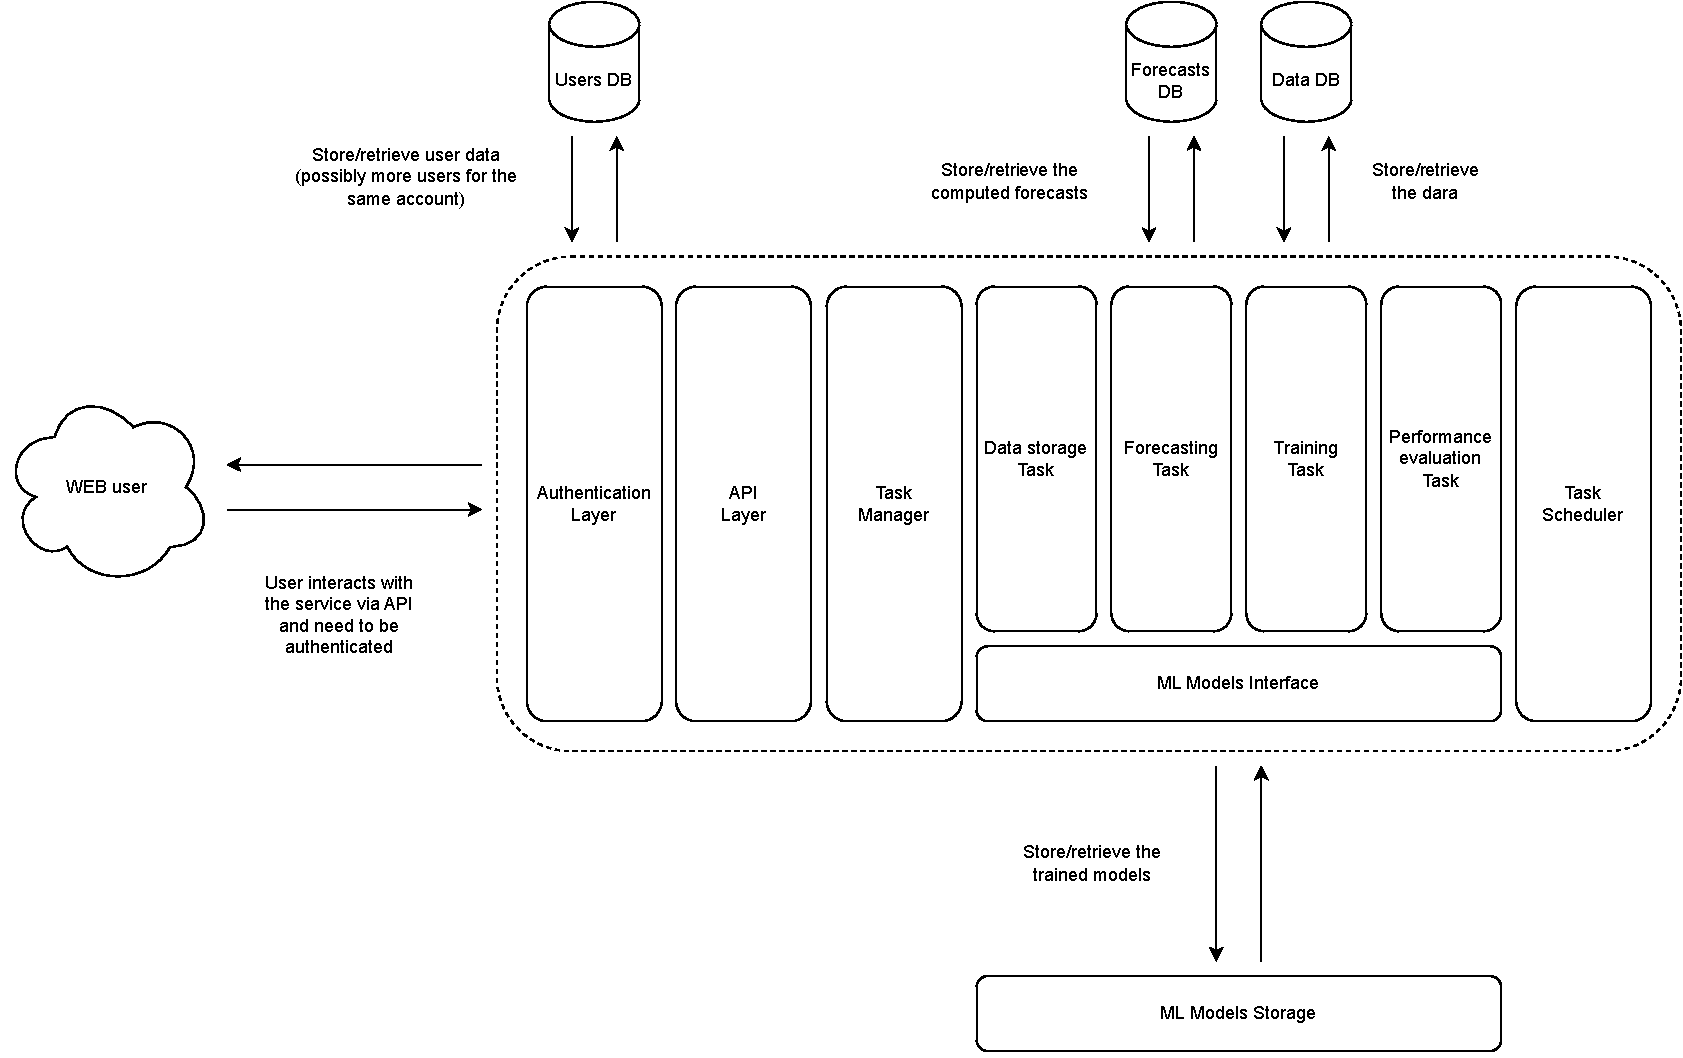
\includegraphics[width=0.9\textwidth]{images/architecture_components}
\caption{The architecture of the proposed system.}
\label{fig:components}
\end{figure}

The use case diagram for the system is presented in figure~\ref{fig:usecase}.
Users can interact with the system via API.
A user must be authenticated and have an account with an active subscription.
Then, he can request the following asynchronous operations:
\begin{itemize}
  \item Append new data with a create or update logic specifying the type of data, it supports the upload of CSV files;
  \item Train new models based on available data for a use case specifying the time granularity (hourly or daily);
  \item Forecast new data for a use case using a specified model or the latest model for a certain time granularity, for a certain starting date and time horizon.
\end{itemize}

In addition, the task scheduler periodically triggers the performance evaluation task for evaluating the performance of the available models and if needed triggering the re-training for having up-to-date models with respect to the user data so that they might perform better on future forecasts.

\begin{figure}[H]
\centering 
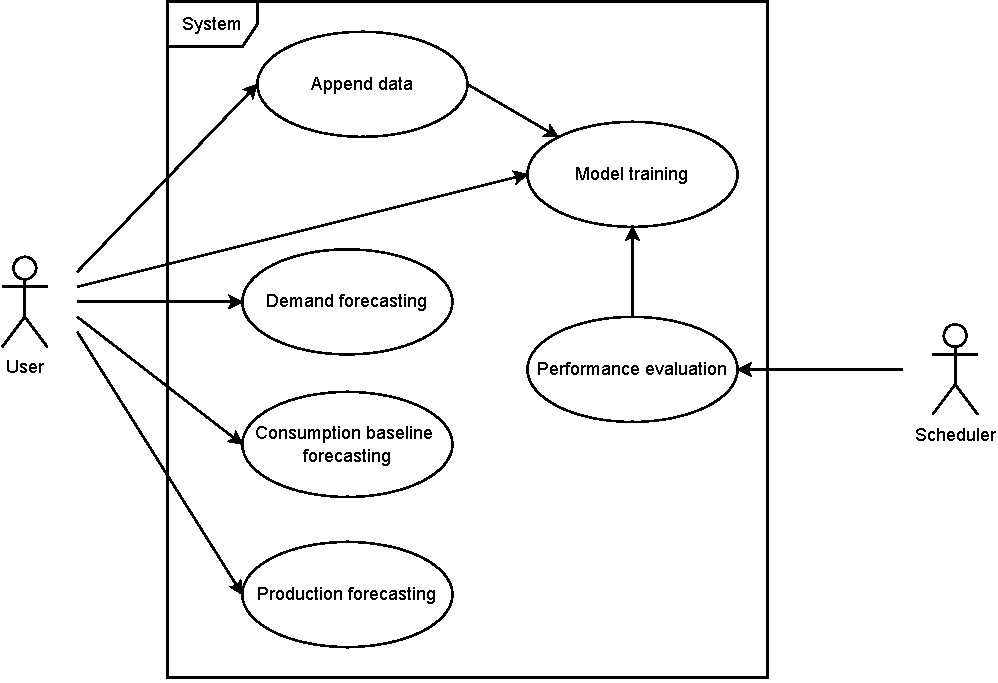
\includegraphics[width=0.6\textwidth]{images/architecture_use_case}
\caption{The use case diagram for the system.}
\label{fig:usecase}
\end{figure}

Figure~\ref{fig:interactions} shows the interactions among the components of the architecture in order to achieve the use cases.
In the specific subsections each the logic for each use case is explained with the relative interactions.

\begin{figure}[H]
\centering 
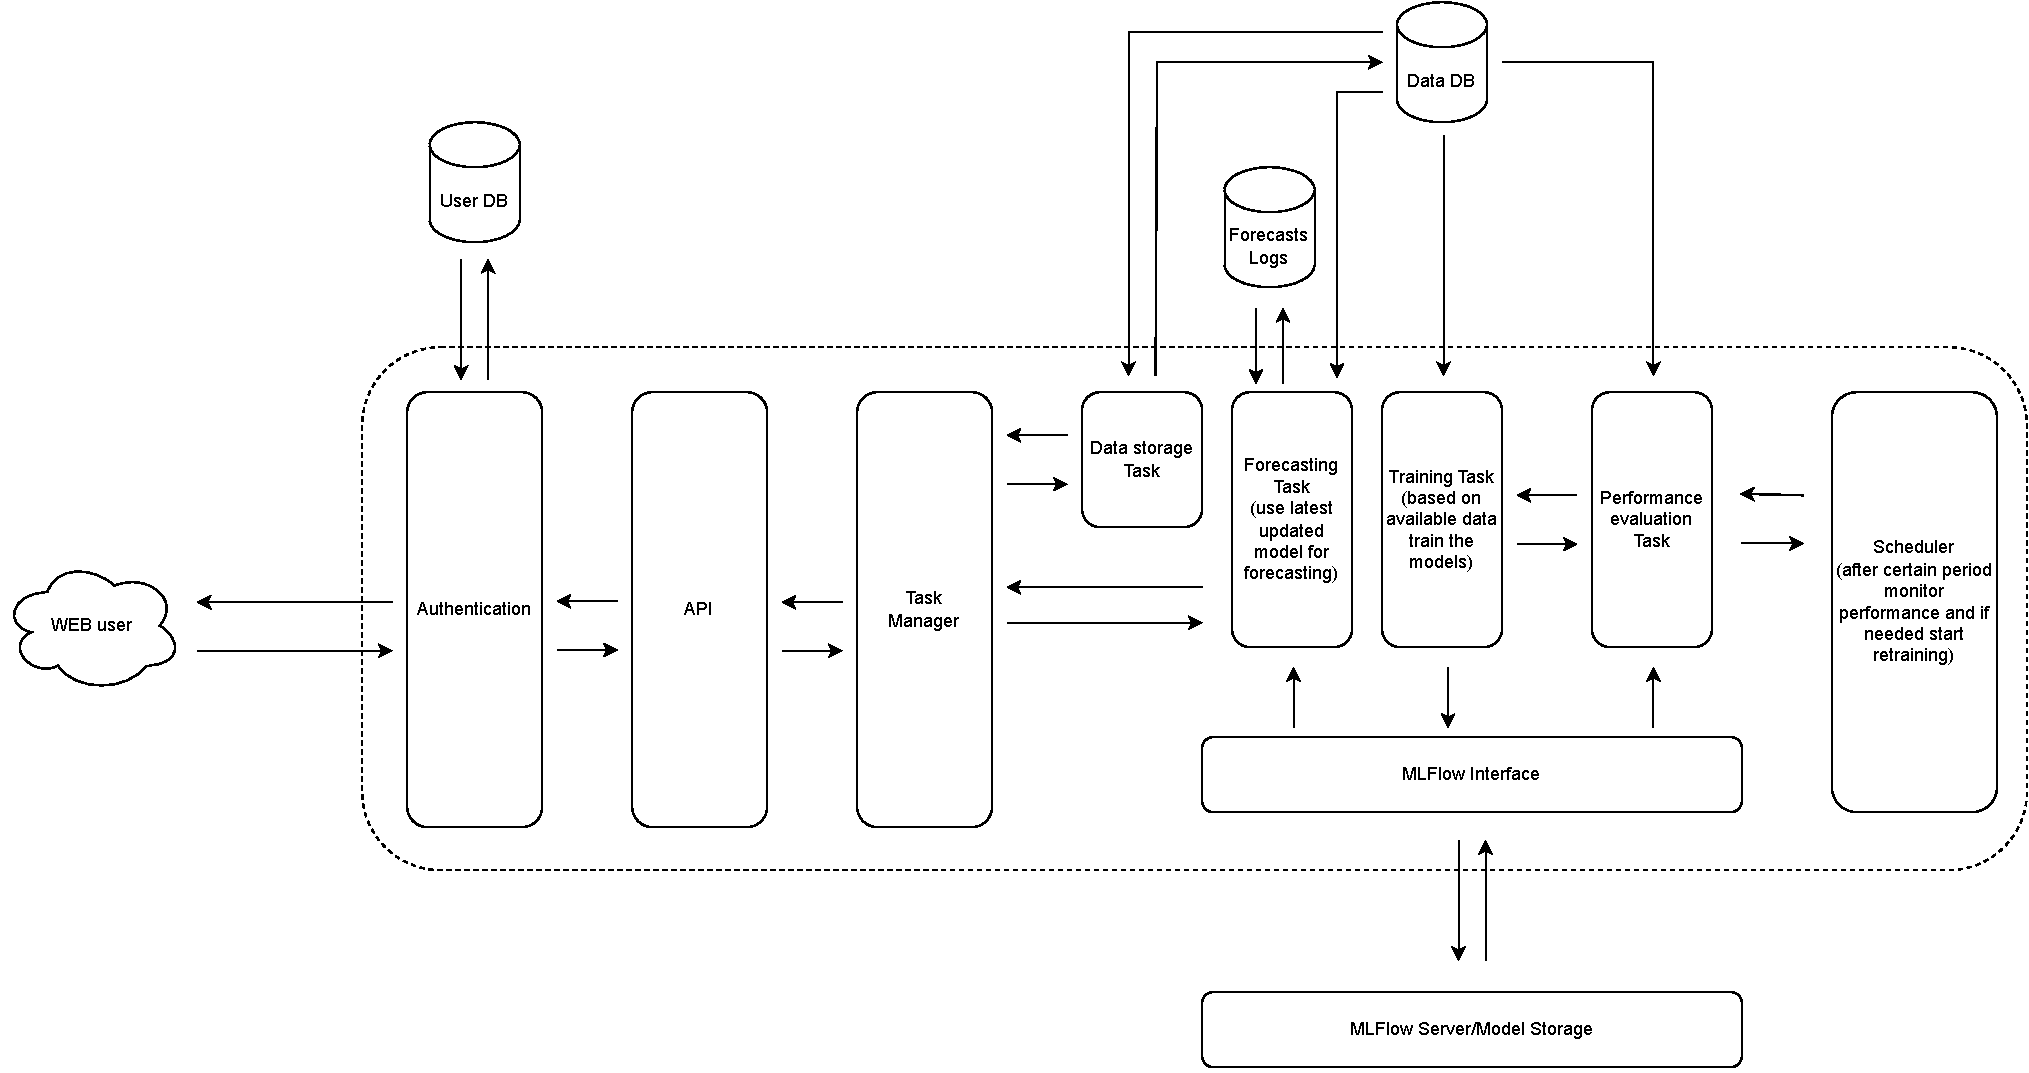
\includegraphics[width=1\textwidth]{images/architecture_interactions}
\caption{The interactions of the components of the proposed system.}
\label{fig:interactions}
\end{figure}


\vspace{0.1 cm}
\subsection{Data loading}
\label{sec:loading}
\vspace{0.1 cm}

The diagram representing the interactions for achieving the data loading use case is presented in figure~\ref{fig:loadinginteractions}.
Describe it ...

\begin{figure}[H]
\centering 
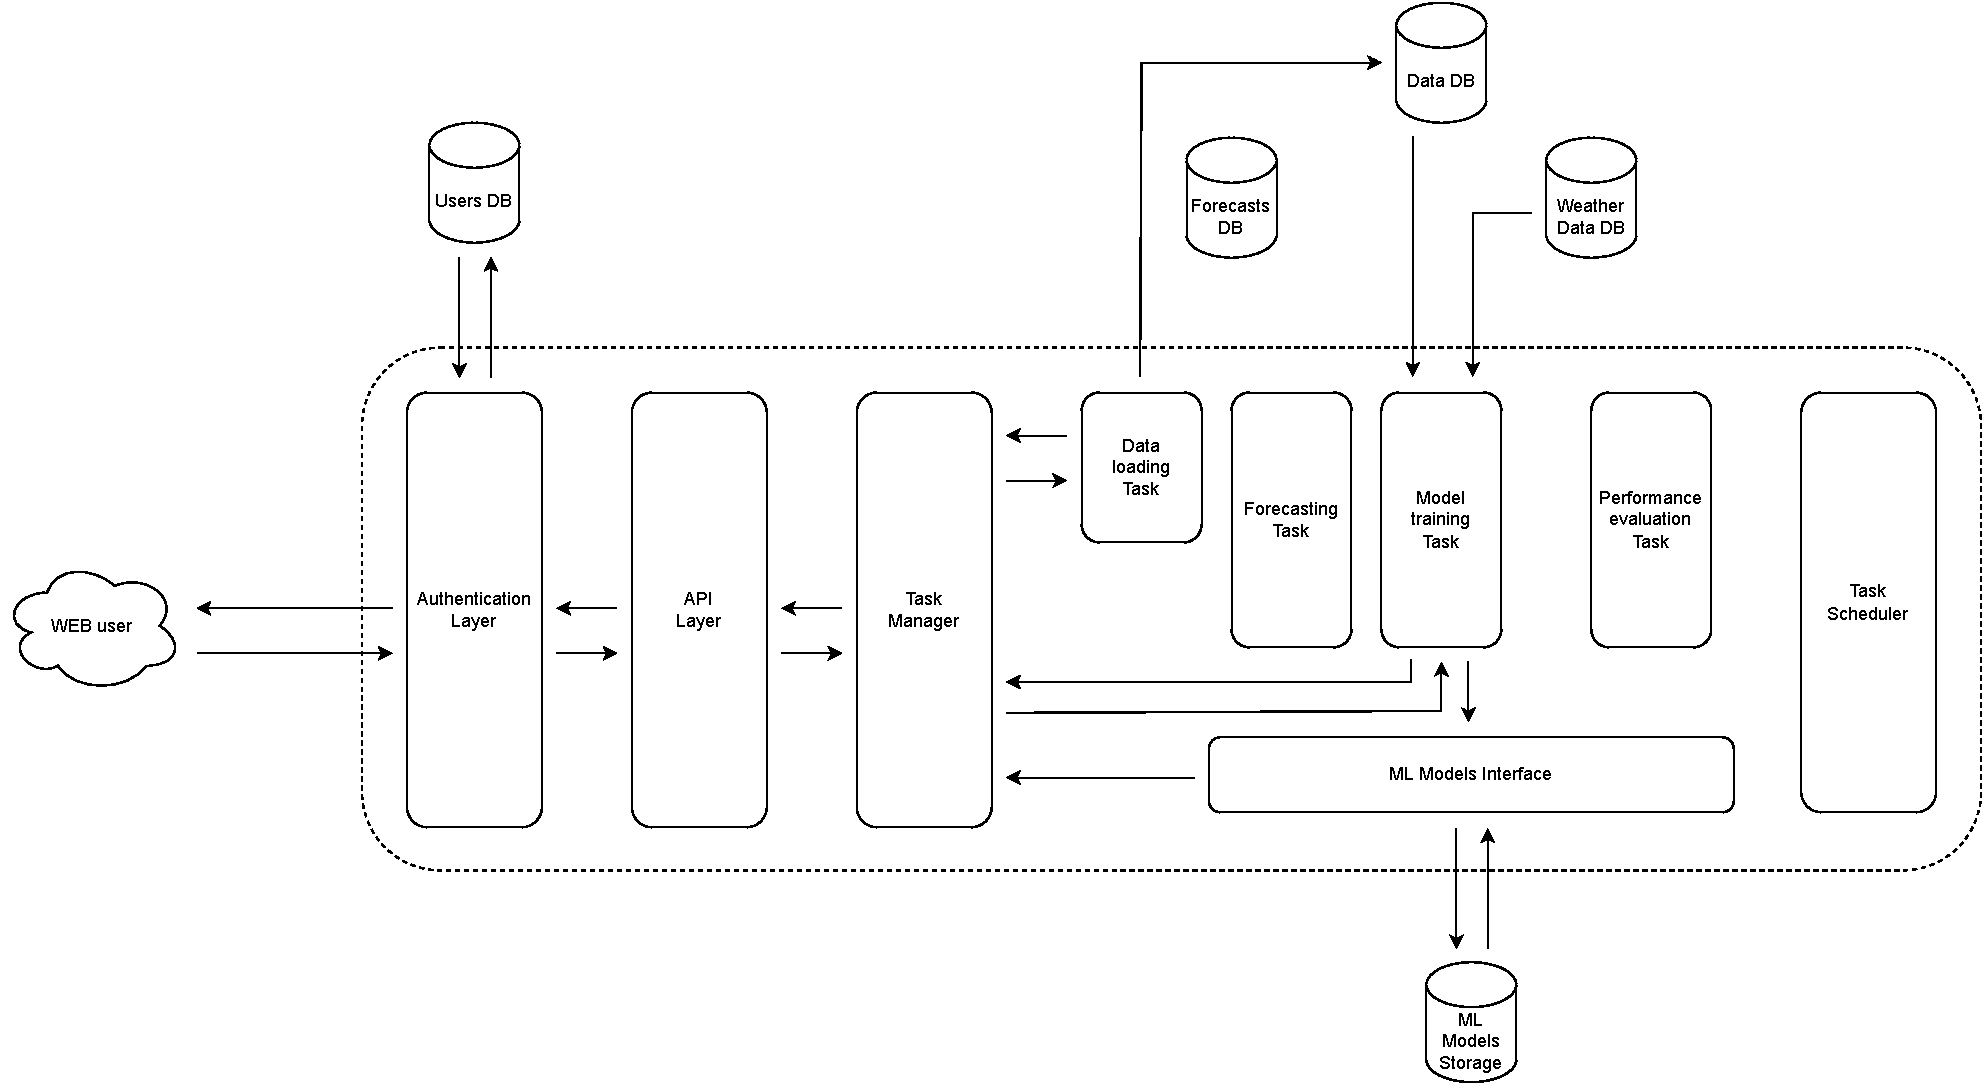
\includegraphics[width=1\textwidth]{images/architecture_data_loading_interactions}
\caption{The interactions of the components for achieving the data loading use case.}
\label{fig:loadinginteractions}
\end{figure}

The diagram representing the data loading flow is presented in figure~\ref{fig:loadingflow}.
Describe it ...

\begin{figure}[H]
\centering 
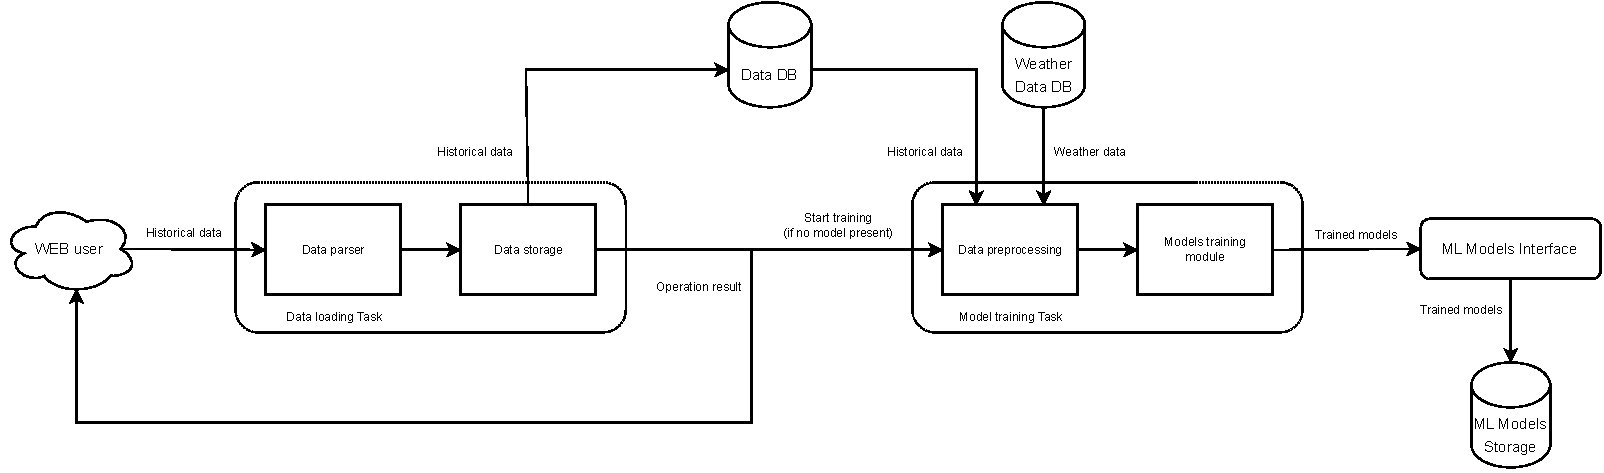
\includegraphics[width=1\textwidth]{images/architecture_data_loading_flow}
\caption{Diagram representing the data loading flow.}
\label{fig:loadingflow}
\end{figure}

The sequence diagram representing the data loading procedure is presented in figure~\ref{fig:loadingsequence}.
Describe it ...

\begin{figure}[H]
\centering 
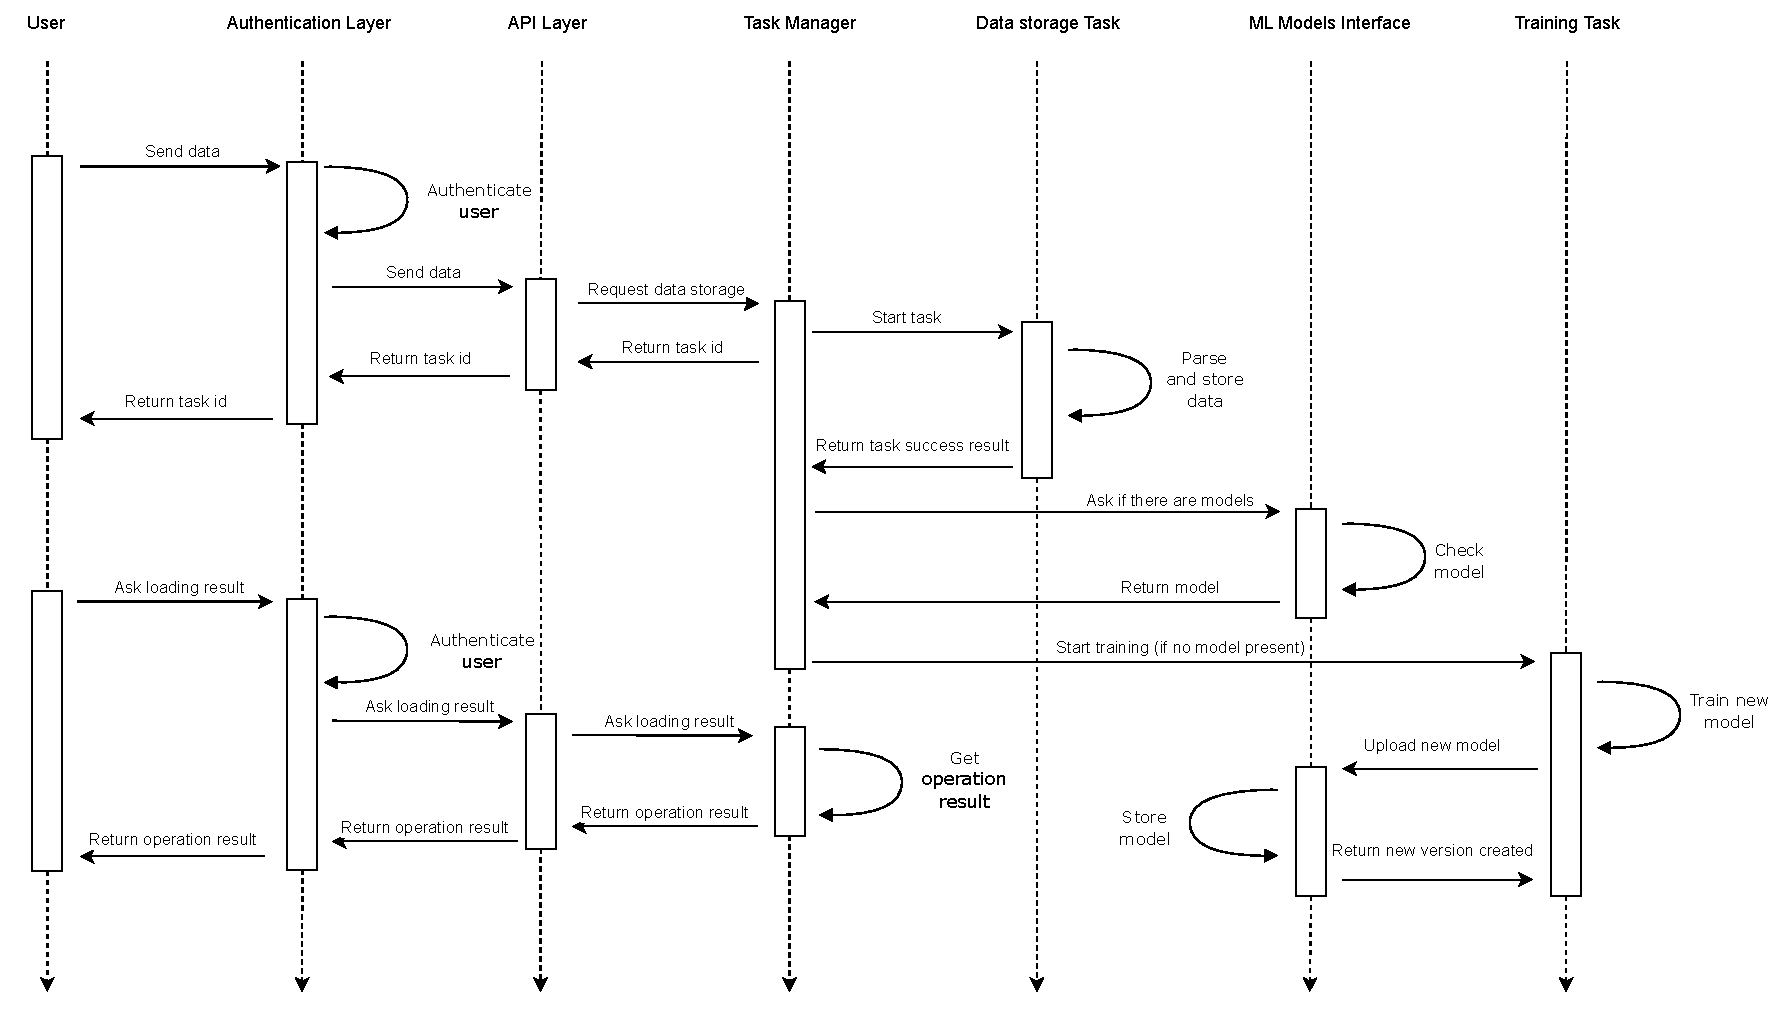
\includegraphics[width=1\textwidth]{images/architecture_data_loading_sequence}
\caption{Sequence diagram of the data loading procedure.}
\label{fig:loadingsequence}
\end{figure}


\vspace{0.1 cm}
\subsection{Training}
\label{sec:training}
\vspace{0.1 cm}

The diagram representing the interactions for achieving the training use case is presented in figure~\ref{fig:traininginteractions}.
Describe it ...

\begin{figure}[H]
\centering 
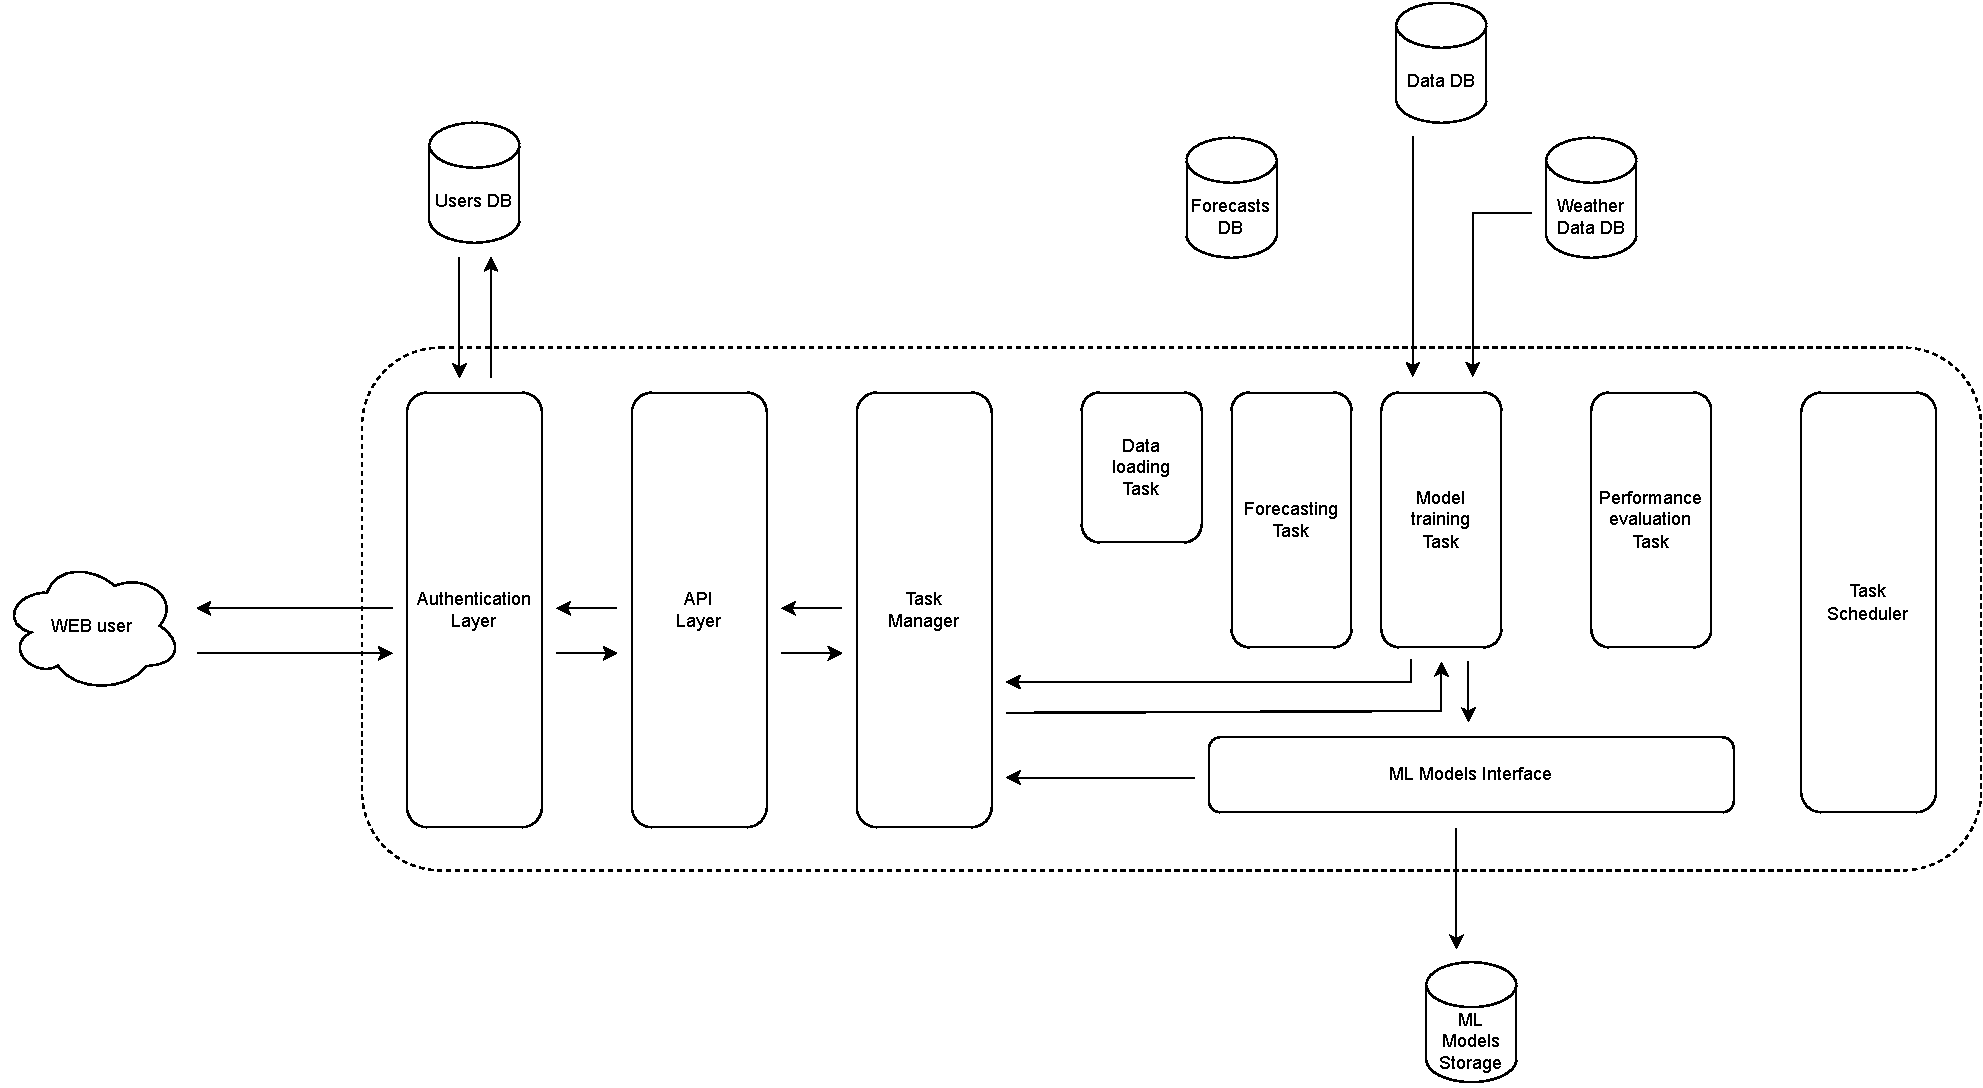
\includegraphics[width=1\textwidth]{images/architecture_training_interactions}
\caption{The interactions of the components for achieving the training use case.}
\label{fig:traininginteractions}
\end{figure}

The diagram representing the training flow is presented in figure~\ref{fig:trainingflow}.
Describe it ...

\begin{figure}[H]
\centering 
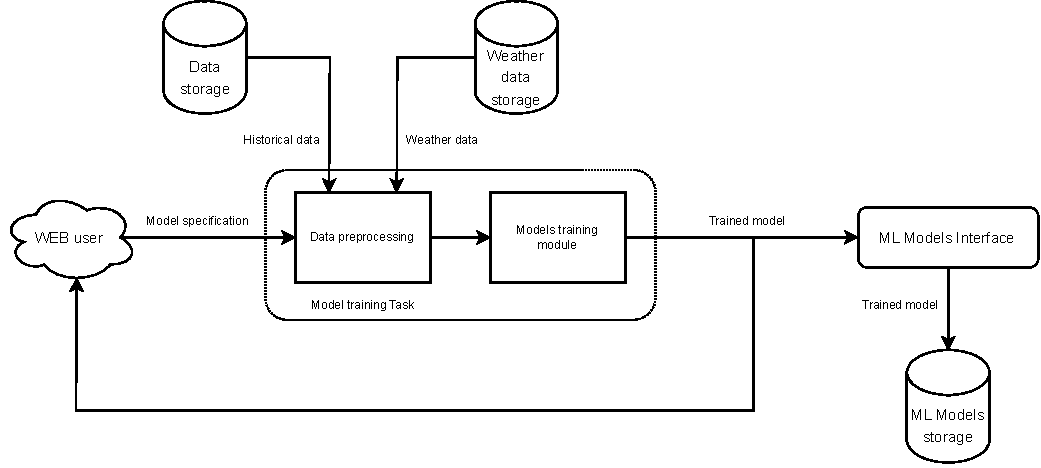
\includegraphics[width=0.7\textwidth]{images/architecture_training_flow}
\caption{Diagram representing the training flow.}
\label{fig:trainingflow}
\end{figure}

The sequence diagram representing the training procedure is presented in figure~\ref{fig:trainingsequence}.
Describe it ...

\begin{figure}[H]
\centering 
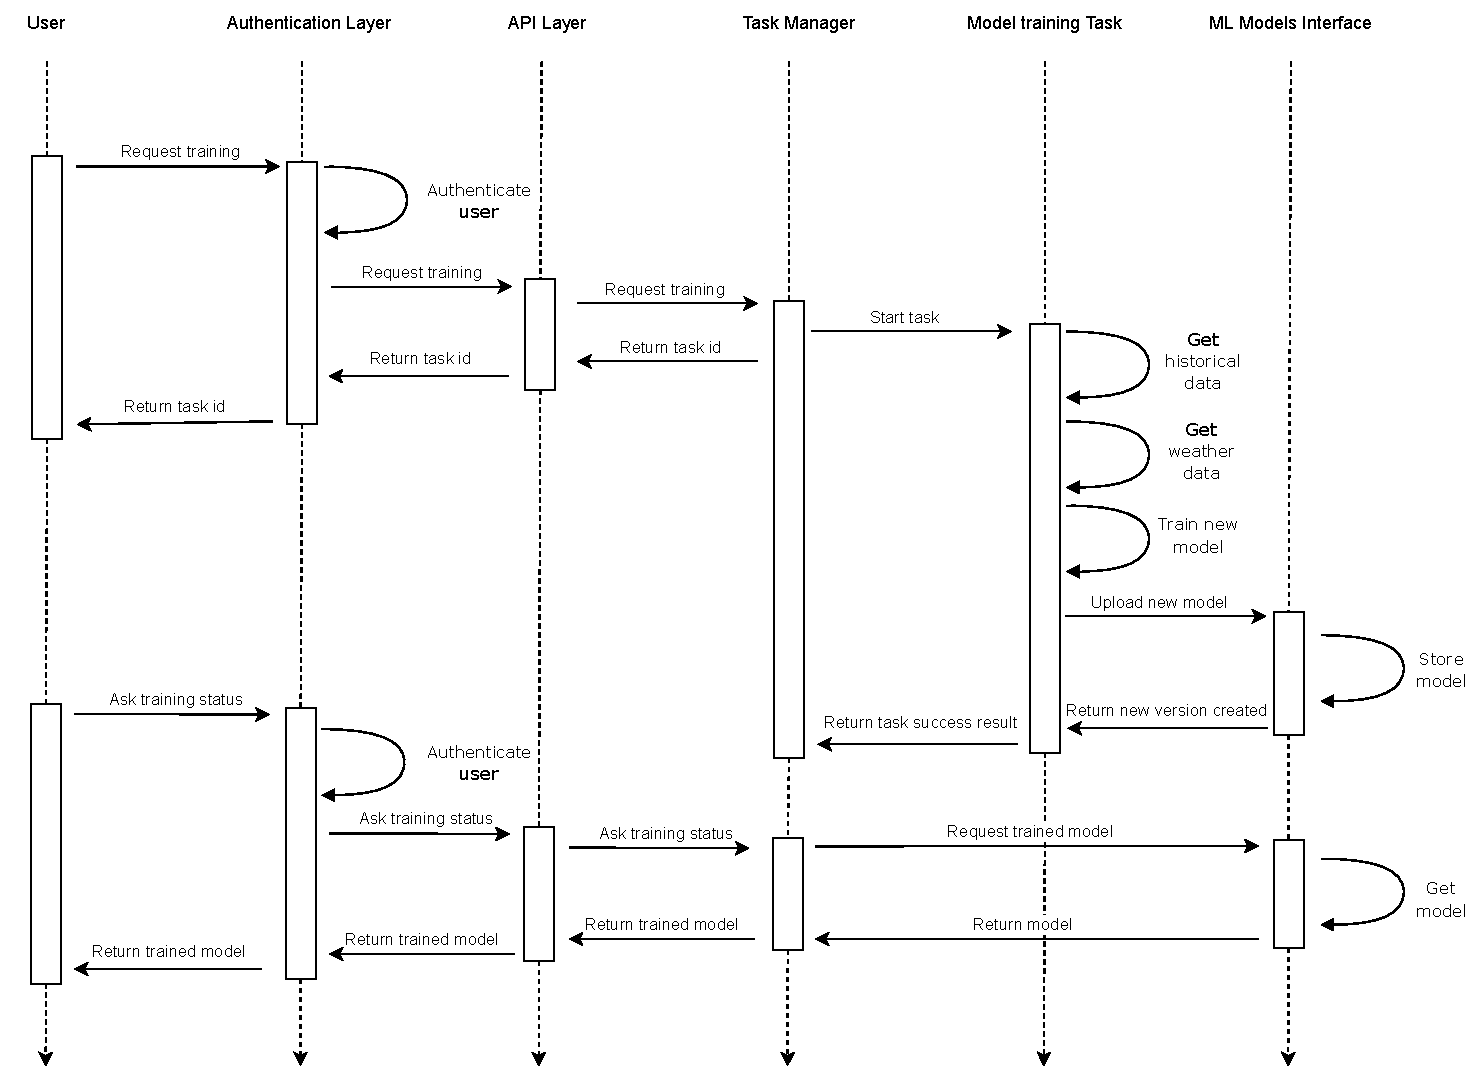
\includegraphics[width=0.8\textwidth]{images/architecture_training_sequence}
\caption{Sequence diagram representing the training procedure.}
\label{fig:trainingsequence}
\end{figure}


\vspace{0.1 cm}
\subsection{Forecasting}
\label{sec:forecasting}
\vspace{0.1 cm}

The diagram representing the interactions for achieving the forecasting use case is presented in figure~\ref{fig:forecastinginteractions}.
Describe it ...

\begin{figure}[H]
\centering 
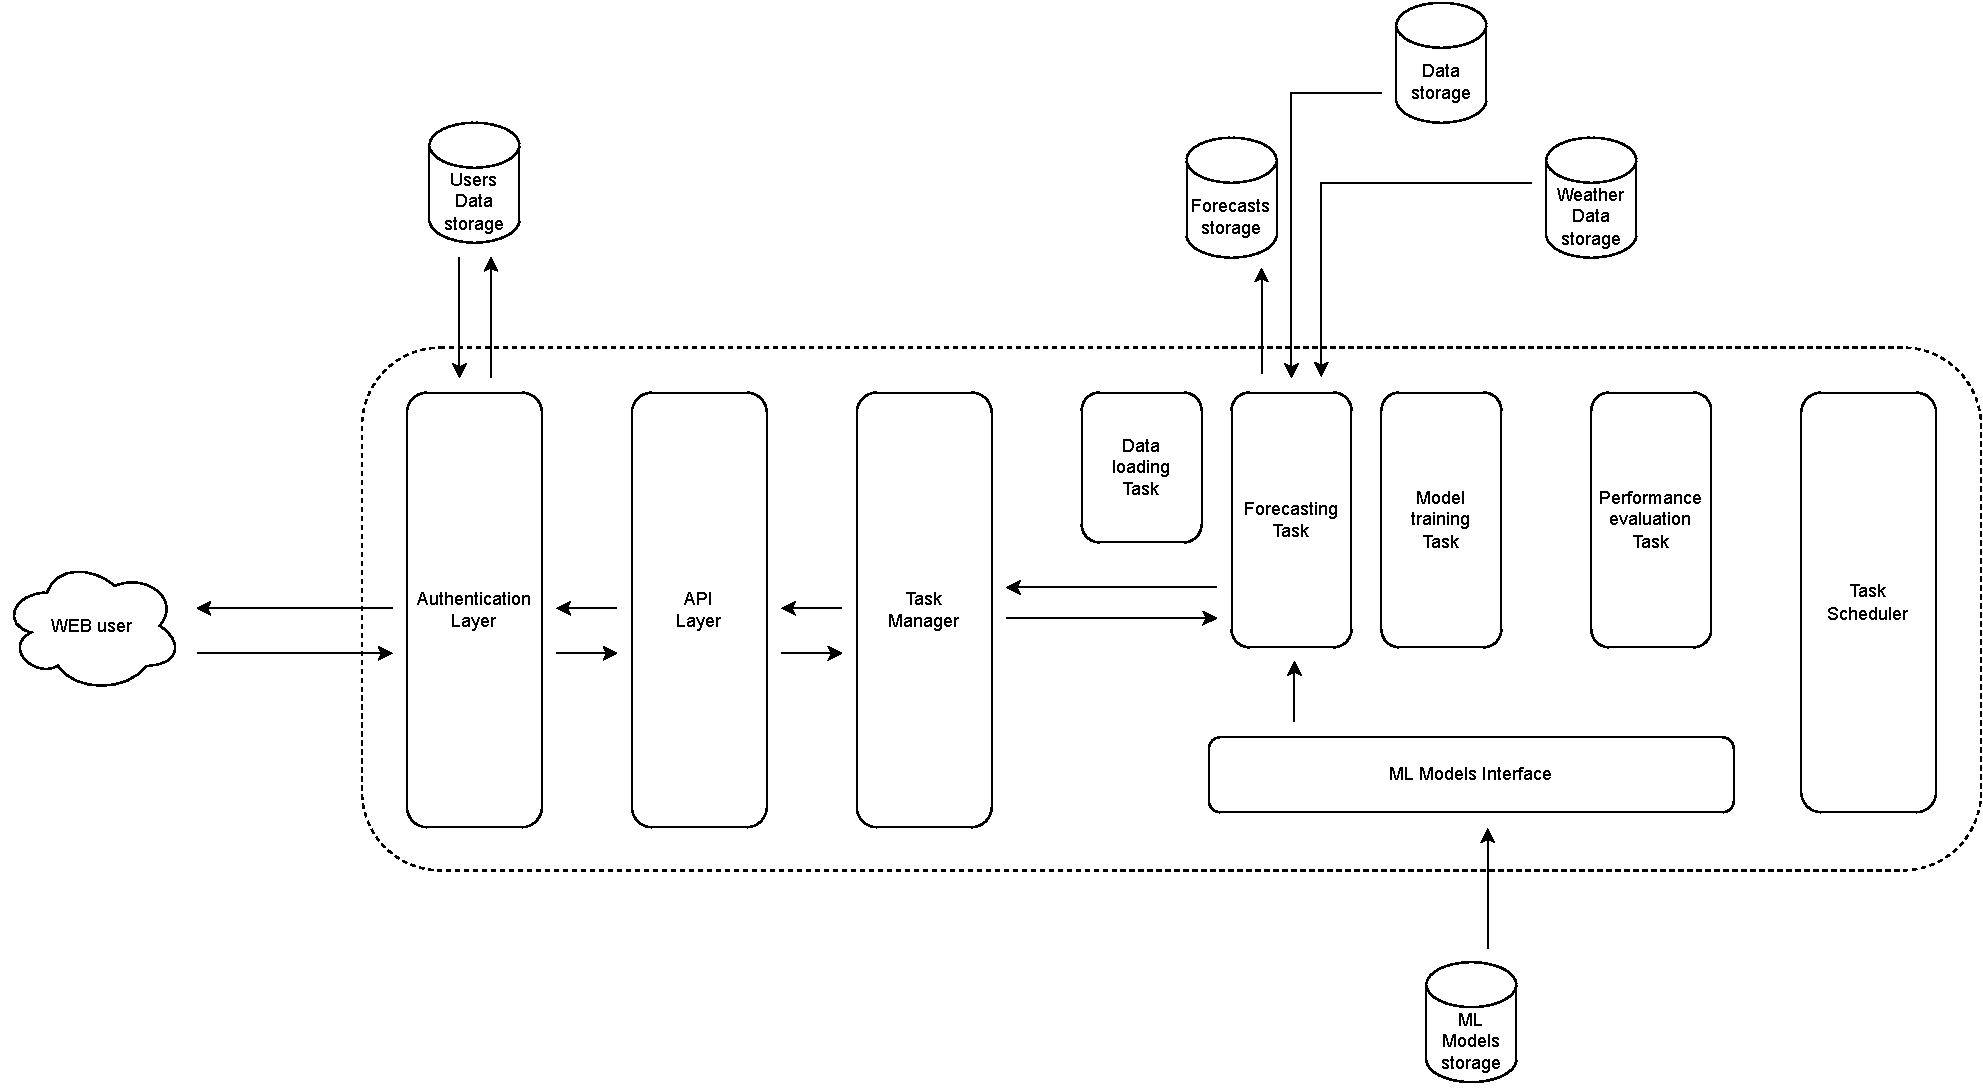
\includegraphics[width=1\textwidth]{images/architecture_forecasting_interactions}
\caption{The interactions of the components for achieving the forecasting use case.}
\label{fig:forecastinginteractions}
\end{figure}

The diagram representing the forecast flow is presented in figure~\ref{fig:forecastflow}.
Describe it ...

\begin{figure}[H]
\centering 
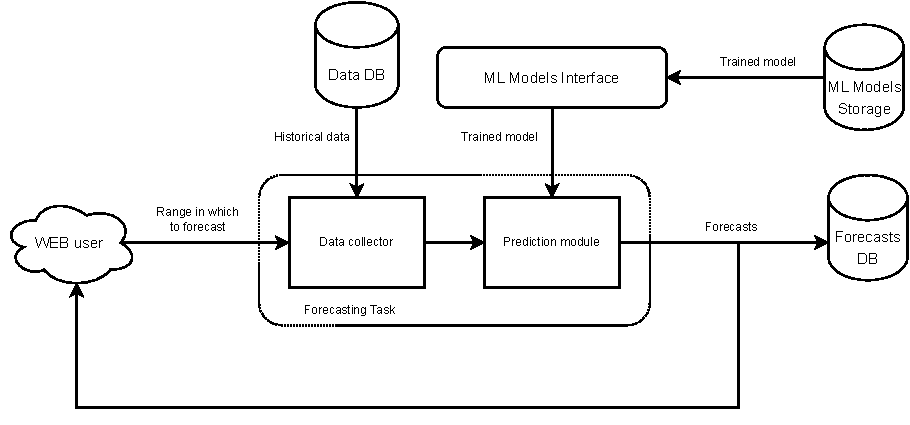
\includegraphics[width=0.6\textwidth]{images/architecture_forecast_flow}
\caption{Diagram representing the forecast flow.}
\label{fig:forecastflow}
\end{figure}

The sequence diagram representing the forecasting procedure is presented in figure~\ref{fig:forecastingsequence}.
Describe it ...

\begin{figure}[H]
\centering 
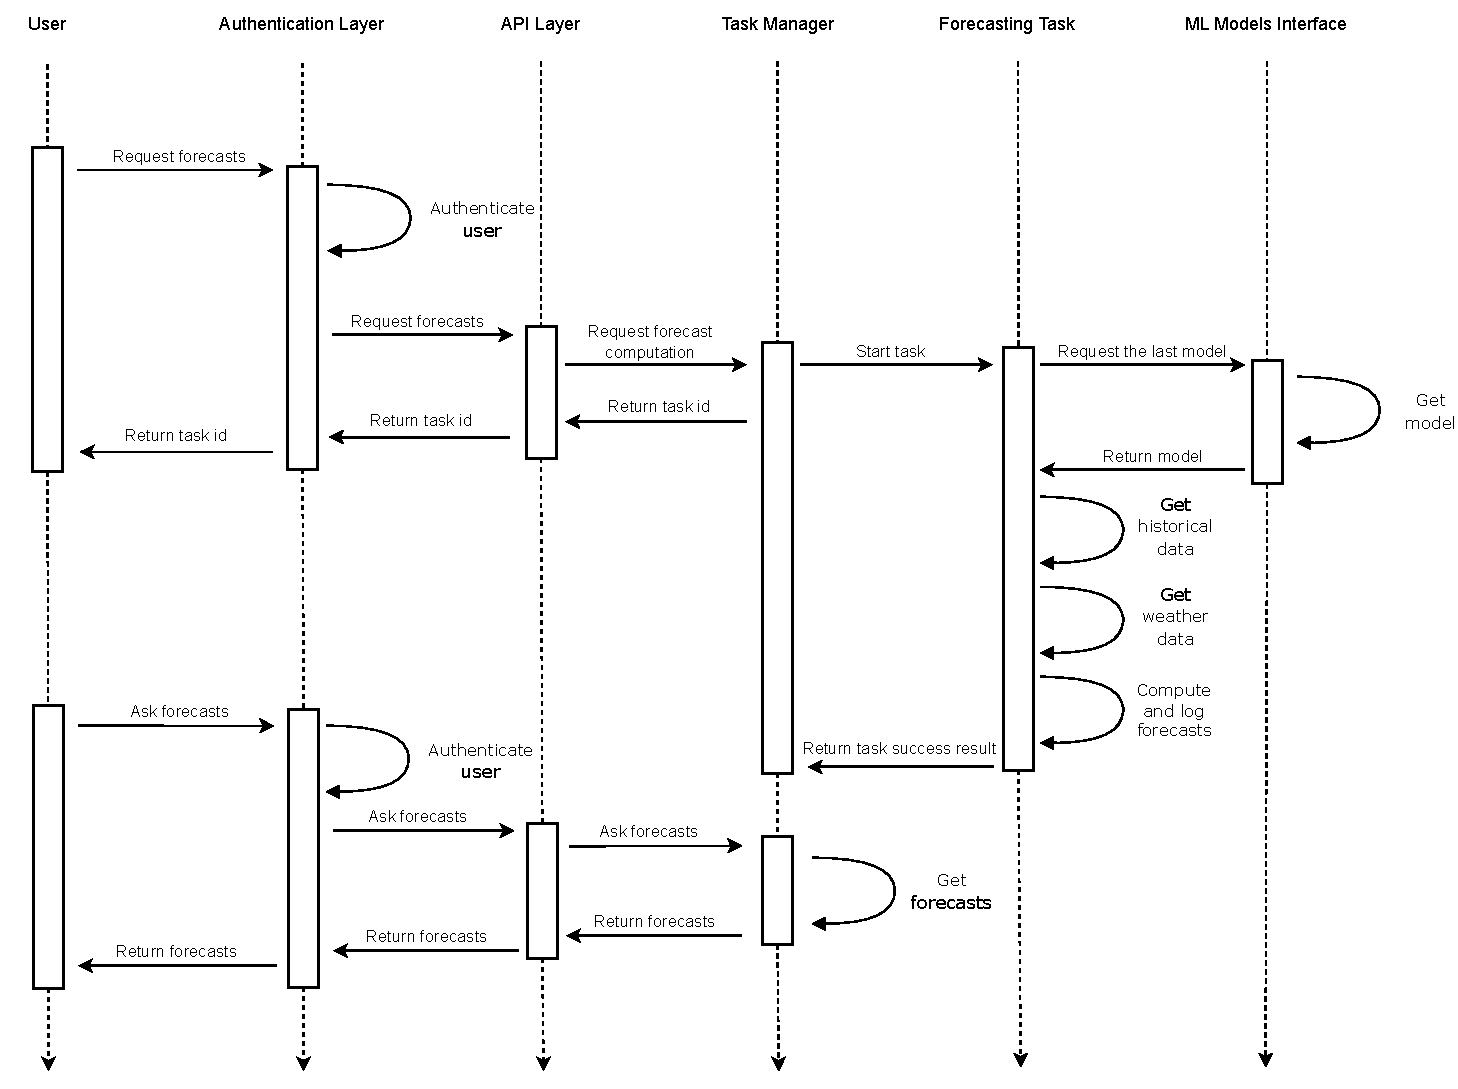
\includegraphics[width=0.8\textwidth]{images/architecture_forecasting_sequence}
\caption{Sequence diagram representing the forecasting procedure.}
\label{fig:forecastingsequence}
\end{figure}


\vspace{0.1 cm}
\subsection{Scheduler}
\label{sec:scheduler}
\vspace{0.1 cm}

The diagram representing the interactions for achieving the task schduler use case is presented in figure~\ref{fig:schedulerinteractions}.
Describe it ...

\begin{figure}[H]
\centering 
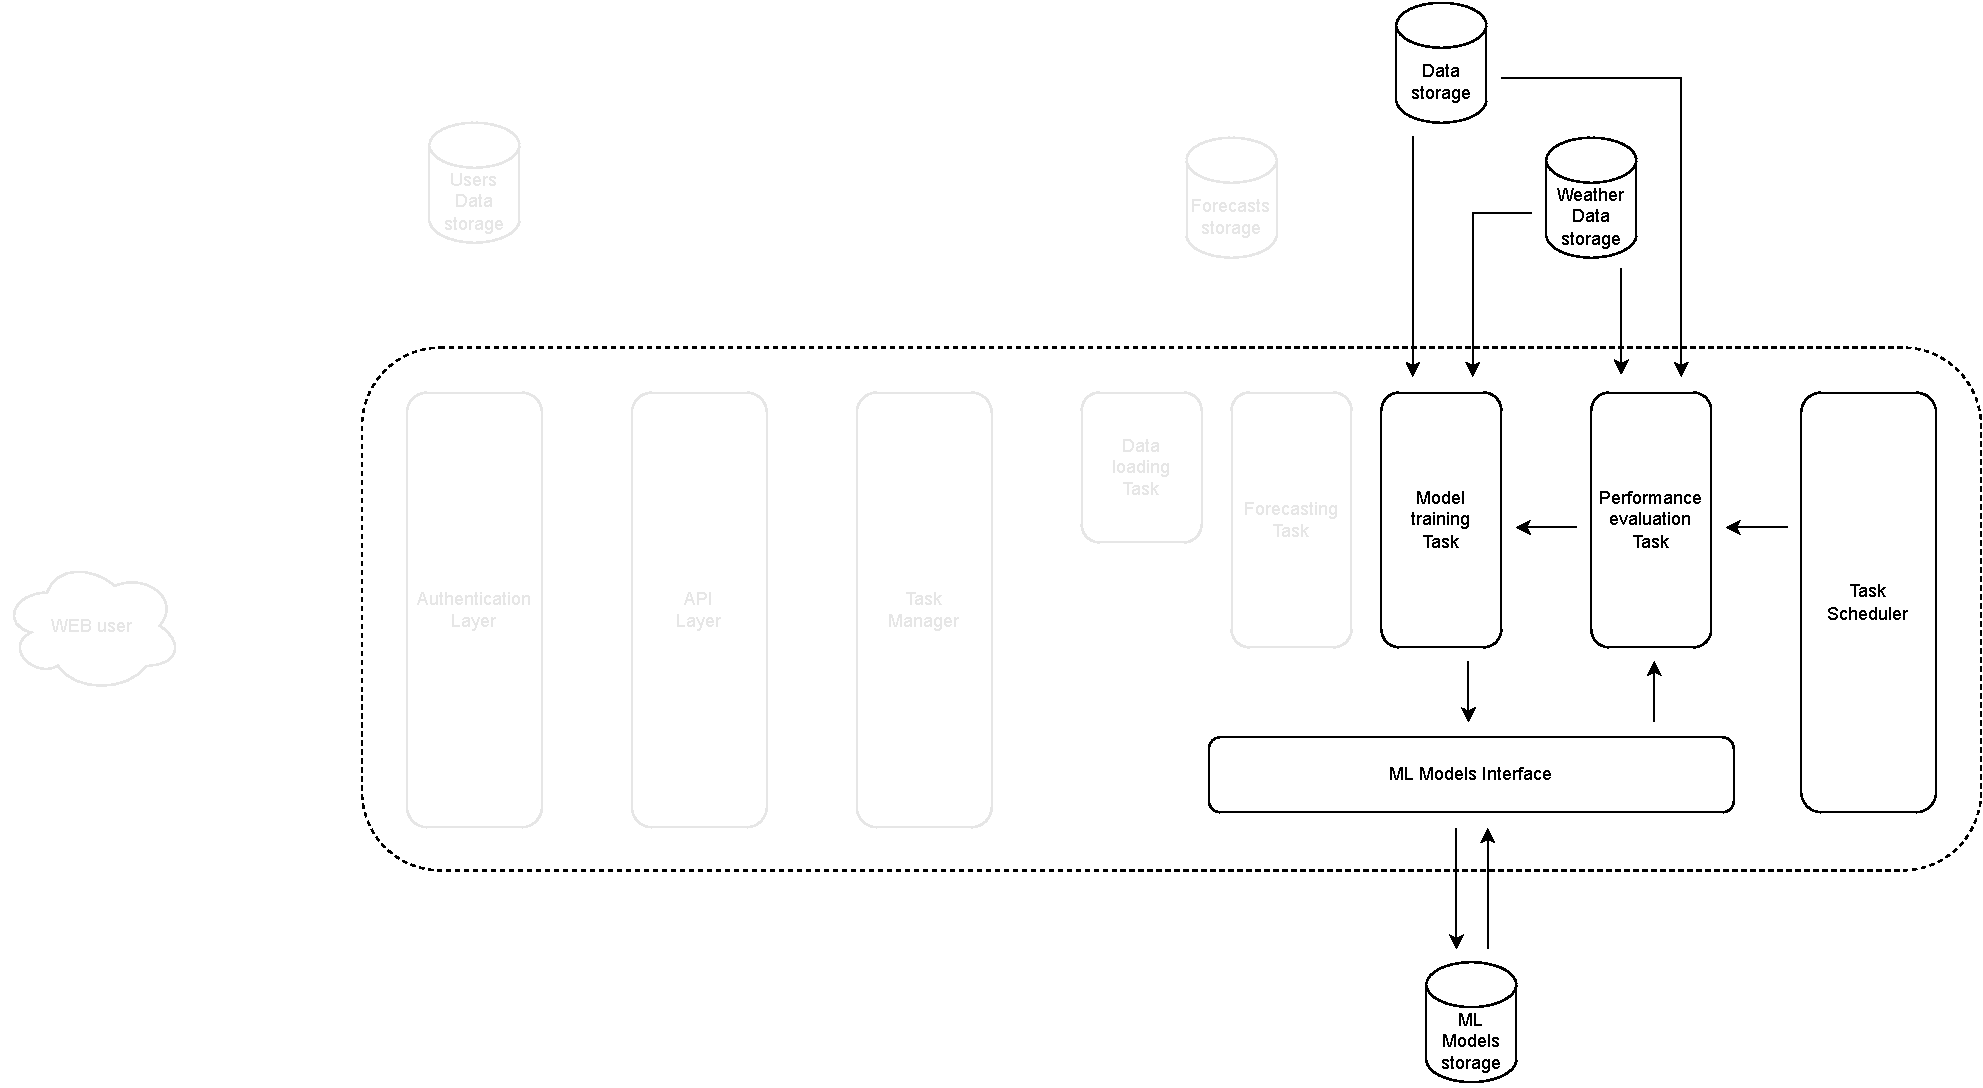
\includegraphics[width=1\textwidth]{images/architecture_scheduler_interactions}
\caption{The interactions of the components for achieving the task schduler use case.}
\label{fig:schedulerinteractions}
\end{figure}

The diagram representing the task scheduler flow is presented in figure~\ref{fig:schedulerflow}.
Describe it ...

\begin{figure}[H]
\centering 
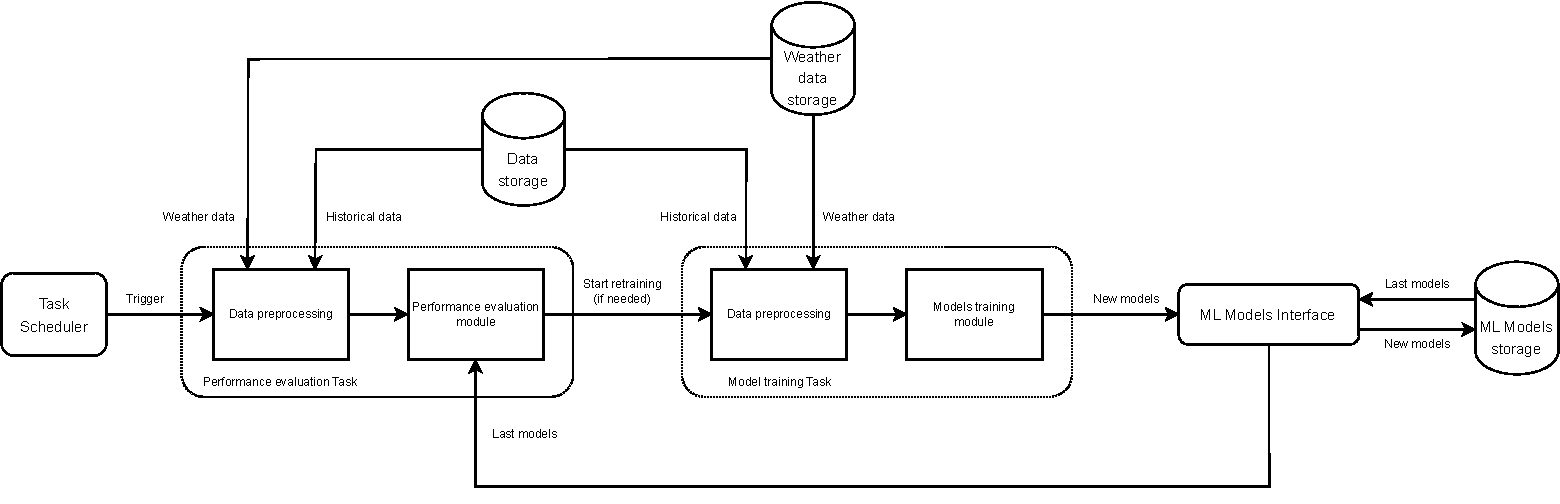
\includegraphics[width=0.8\textwidth]{images/architecture_scheduler_flow}
\caption{Diagram representing the task scheduler flow.}
\label{fig:schedulerflow}
\end{figure}

The sequence diagram representing the task scheduler procedure is presented in figure~\ref{fig:schedulersequence}.
Describe it ...

\begin{figure}[H]
\centering 
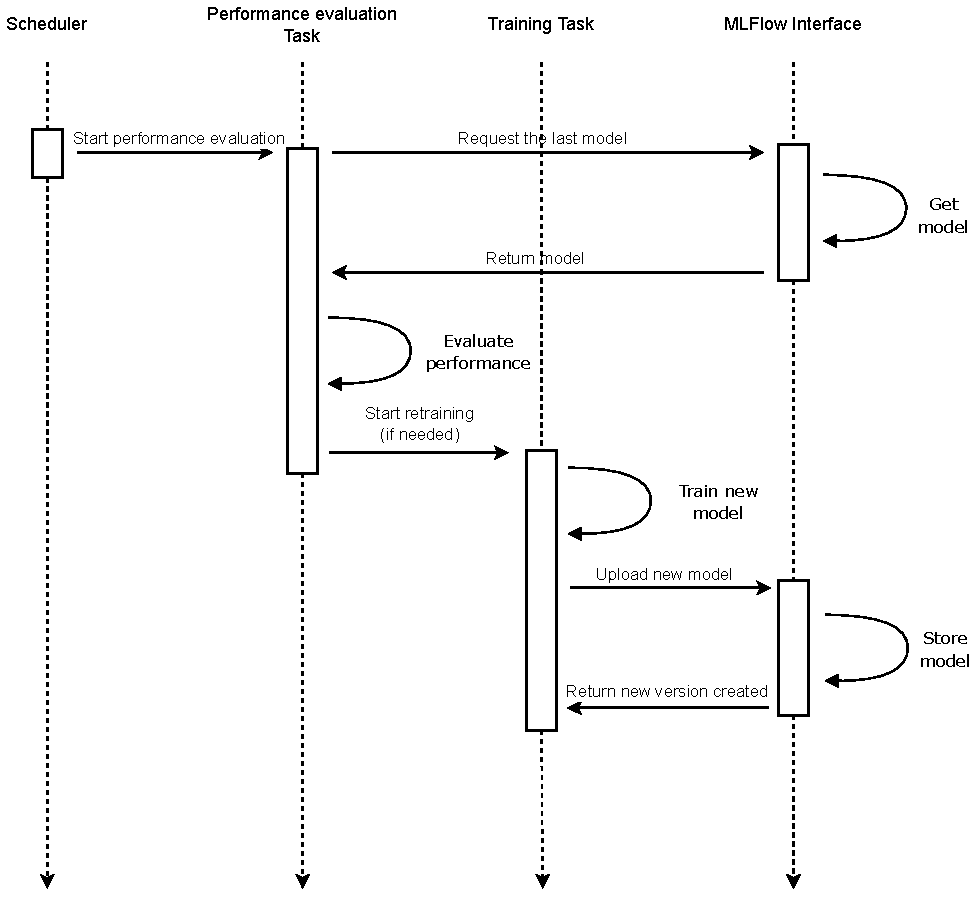
\includegraphics[width=0.6\textwidth]{images/architecture_scheduler_sequence}
\caption{Sequence diagram representing the task scheduler procedure.}
\label{fig:schedulersequence}
\end{figure}


\section{System's common components}
\label{sec:components}
\vspace{0.2 cm}

Describe the system's common components between the various tasks ...

Describe Data Parser/Preprocessing, Enrichment, Model Training Procedure, Prediction, ...


\section{Electricity demand forecasting module}
\label{sec:demandmodel}
\vspace{0.2 cm}

Describe the electricity demand forecasting module ...

How the module works, what contains, describe the models used for the task-specific and then report also in the sections below if they are common, ...

The system model training schematic representation for electricity demand forecasting is presented in figure~\ref{fig:modeltrainingdemand}.

\begin{figure}[H]
\centering 
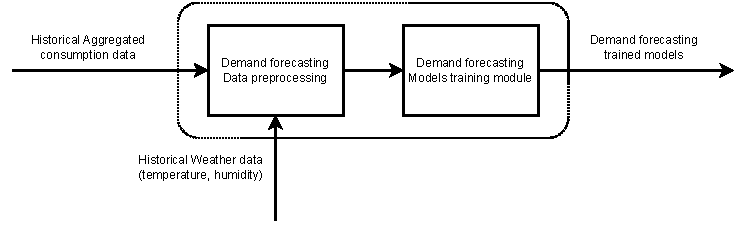
\includegraphics[width=0.7\textwidth]{images/system_model_training_demand}
\caption{The system model training schematic representation for electricity demand forecasting.}
\label{fig:modeltrainingdemand}
\end{figure}

The system model forecasting schematic representation for electricity demand forecasting is presented in figure~\ref{fig:modelforecastingdemand}.

\begin{figure}[H]
\centering 
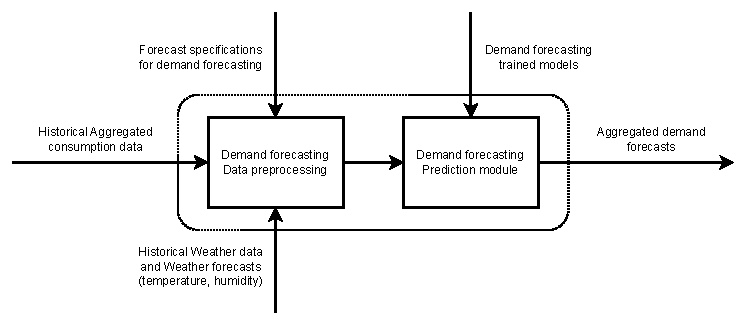
\includegraphics[width=0.7\textwidth]{images/system_model_forecasting_demand}
\caption{The system model forecasting schematic representation for electricity demand forecasting.}
\label{fig:modelforecastingdemand}
\end{figure}


\section{Consumption baseline forecasting module}
\label{sec:baselinemodel}
\vspace{0.2 cm}

Describe the consumption baseline forecasting module ...

The system model training schematic representation for consumption baseline forecasting is presented in figure~\ref{fig:modeltrainingbaseline}.

\begin{figure}[H]
\centering 
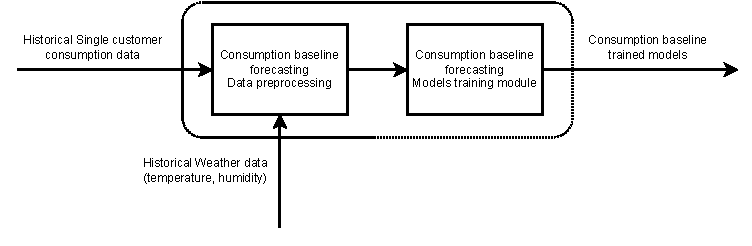
\includegraphics[width=0.7\textwidth]{images/system_model_training_baseline}
\caption{The system model training schematic representation for consumption baseline forecasting.}
\label{fig:modeltrainingbaseline}
\end{figure}

The system model forecasting schematic representation for consumption baseline forecasting is presented in figure~\ref{fig:modelforecastingbaseline}.

\begin{figure}[H]
\centering 
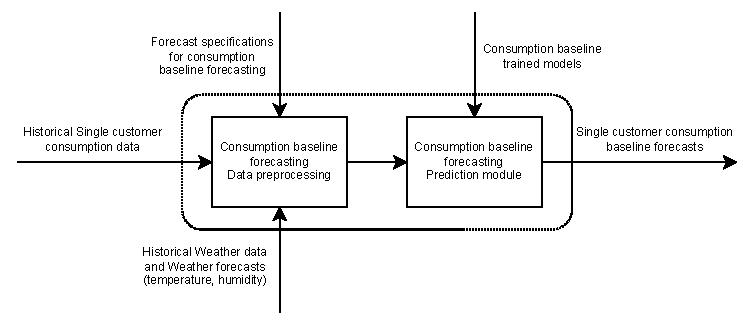
\includegraphics[width=0.7\textwidth]{images/system_model_forecasting_baseline}
\caption{The system model forecasting schematic representation for consumption baseline forecasting.}
\label{fig:modelforecastingbaseline}
\end{figure}


\section{Electricity production forecasting module}
\label{sec:productionmodel}
\vspace{0.2 cm}

Describe the electricity production forecasting module ...

The system model training schematic representation for electricity production forecasting is presented in figure~\ref{fig:modeltrainingproduction}.

\begin{figure}[H]
\centering 
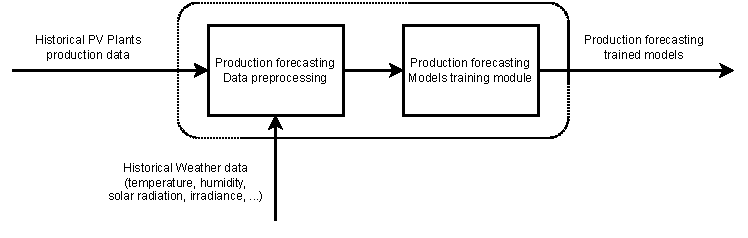
\includegraphics[width=0.7\textwidth]{images/system_model_training_production}
\caption{The system model training schematic representation for electricity production forecasting.}
\label{fig:modeltrainingproduction}
\end{figure}

The system model forecasting schematic representation for electricity production forecasting is presented in figure~\ref{fig:modelforecastingproduction}.

\begin{figure}[H]
\centering 
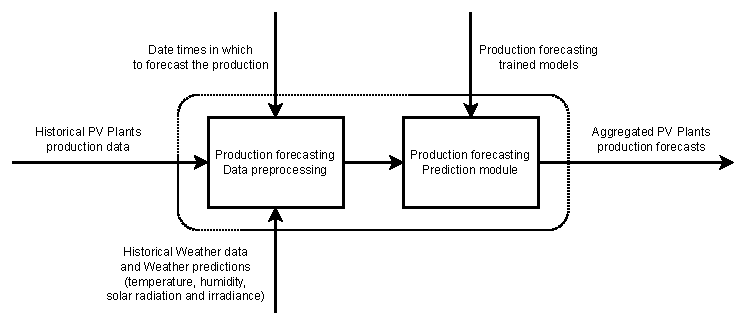
\includegraphics[width=0.7\textwidth]{images/system_model_forecasting_production}
\caption{The system model forecasting schematic representation for electricity production forecasting.}
\label{fig:modelforecastingproduction}
\end{figure}

      \newpage
      \afterpage{\null\thispagestyle{empty}\clearpage}

      \chapter{Prototype Implementation}
\label{cha:implementation}
\vspace{0.4 cm}

This chapter presents which components of the system have been implemented and how.
Only a subset of the components of the designed architecture in chapter~\ref{cha:system} have been implemented.
This is because a prototype was developed as a Proof of Concept (PoC) with a focus on key components for validating the core system functionalities for each specific use case.
These are the training of models, the forecast of new data, and the evaluation of the performance of the developed models.
The remaining components were not implemented since they were not crucial for having a working system, in fact, the overall architecture was designed in order to build a Software as a Service (SaaS) on the implemented core system functionalities.

The first section describes the implementation of the system's common components across the various specific use cases and the others explain the implementation details of the use case-specific modules.
After this chapter, it will be clear how the system prototype was implemented and ready for validation and testing phases, which are discussed in chapter~\ref{cha:evaluation}.


\section{System's common components}
\label{sec:componentsimpl}
\vspace{0.2 cm}

The effectively implemented components of the architecture designed for the proposed system are reported in figure~\ref{fig:implementationcomponents}.
The interactions among them are reported in figure~\ref{fig:implementationinteractions}.

\begin{figure}[H]
\centering
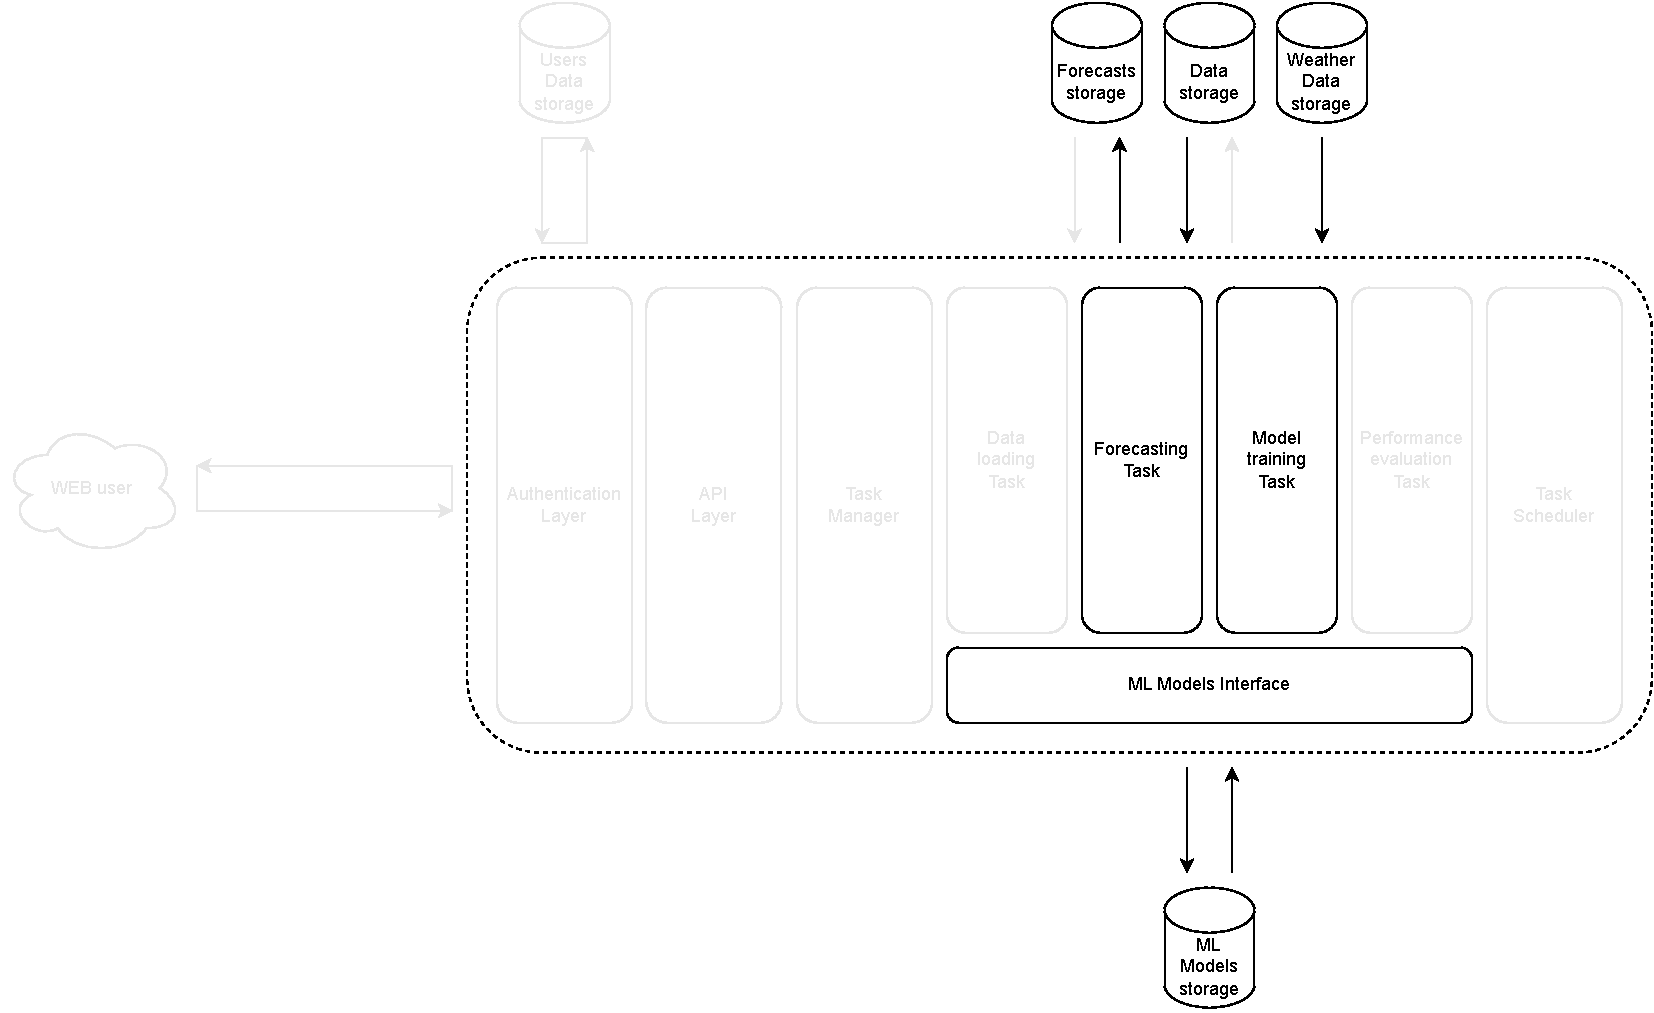
\includegraphics[width=0.9\textwidth]{images/implementation_components}
\caption{The effectively implemented components of the architecture designed for the proposed system.}
\label{fig:implementationcomponents}
\end{figure}

The ML model interface was implemented using the pickle library\footnote{ \url{https://docs.python.org/3/library/pickle.html} } for interfacing with the ML models storage for storing the ML models and retrieving the stored ones making them available for prediction and evaluation.
The use of the MLflow client\footnote{ \url{https://mlflow.org/} } was thought of as a possible interface in the complete system integration for interfacing with the ML models storage.

The model training task trains new models based on available data for the specific use case.
The details about the models and their training process for each specific use case are reported in the dedicated sections.

The forecasting task forecasts future data using the available models for the specific use case.
The details about the models and their forecasting process for each specific use case are reported in the dedicated sections.

The performance evaluation task evaluates the performance of the available models for the specific use case.
The details about the performance evaluation process for each specific use case are reported in chapter~\ref{cha:evaluation}.

\begin{figure}[H]
\centering
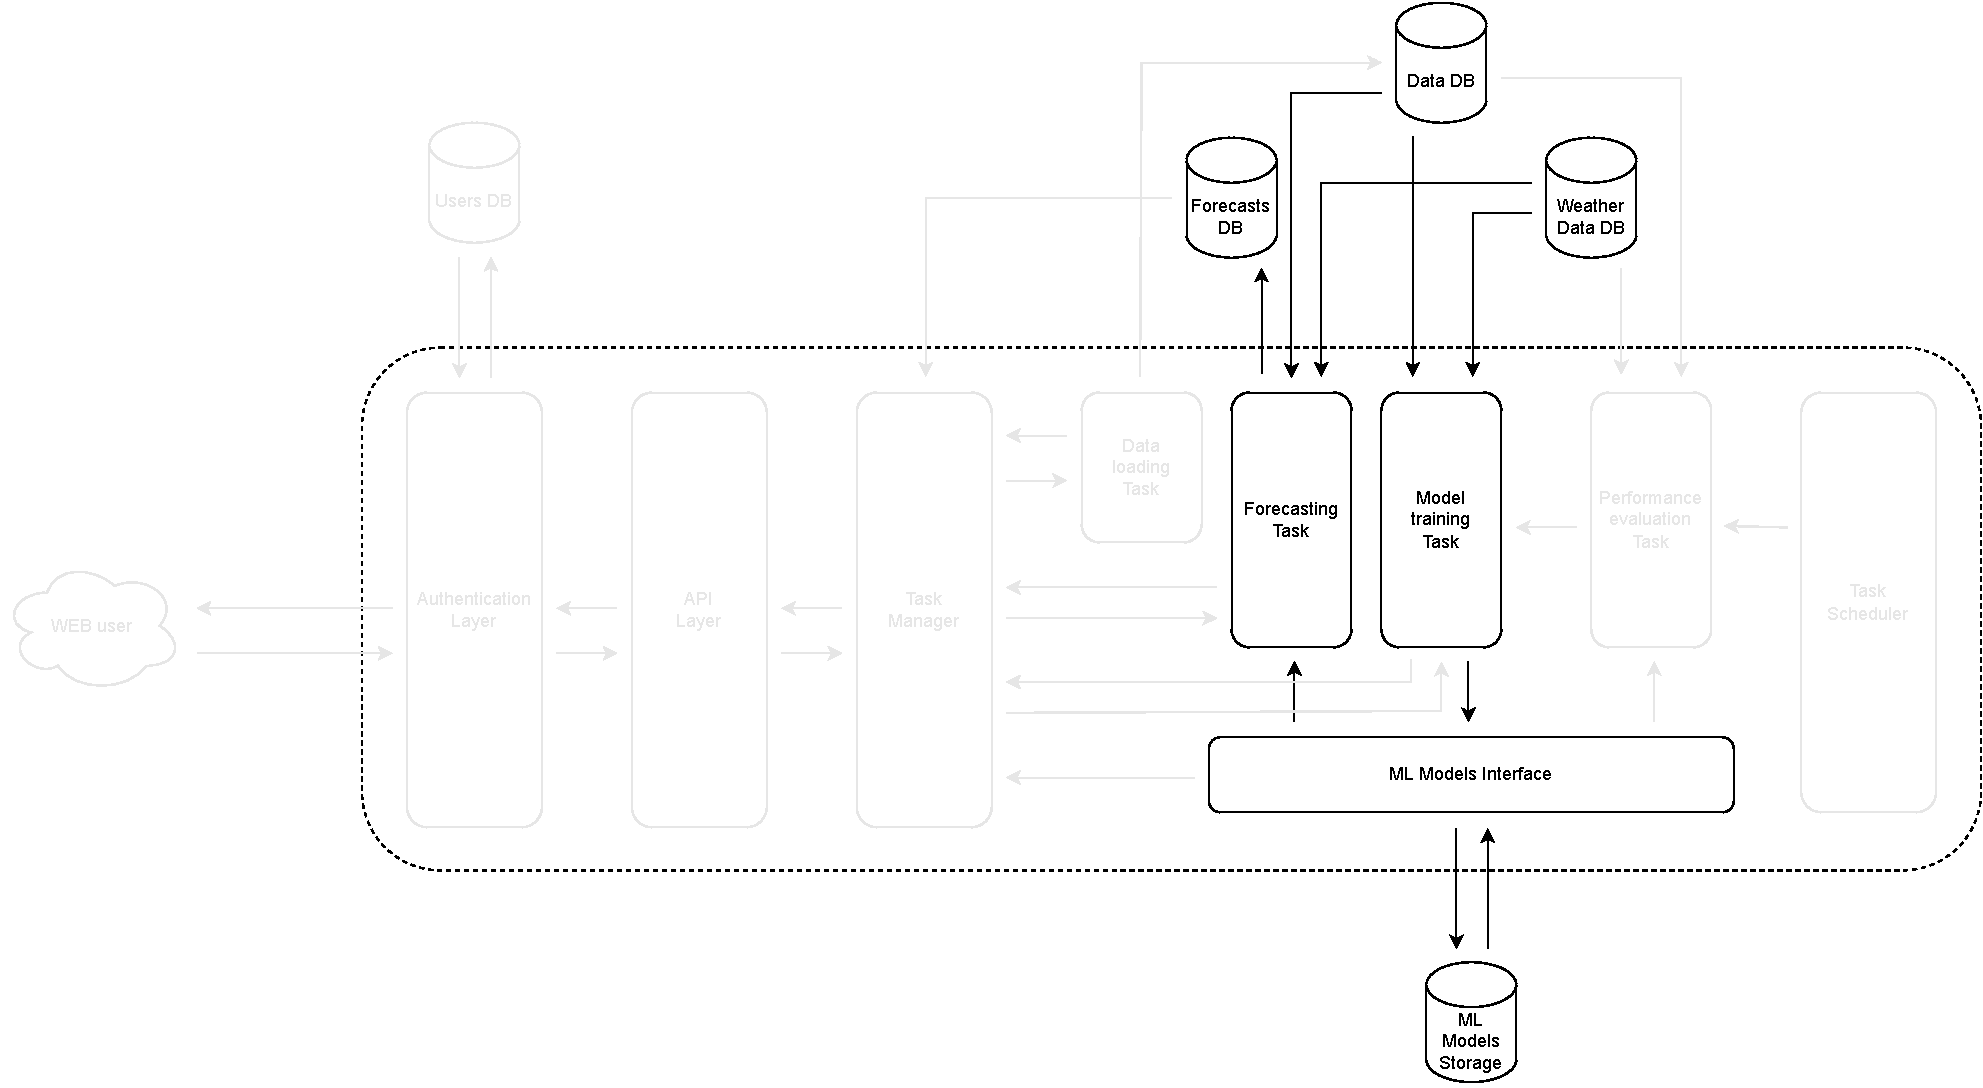
\includegraphics[width=1\textwidth]{images/implementation_interactions}
\caption{The interactions among the effectively implemented components of the architecture designed for the proposed system.}
\label{fig:implementationinteractions}
\end{figure}

The system interacts with the following external components: data storage, weather data storage, ML models storage, and forecasts storage.

The data storage consists of CSV files containing the data for the different use cases, which are loaded using the pandas library\footnote{ \url{https://pandas.pydata.org/} }.
InfluxDB\footnote{ \url{https://www.influxdata.com/} } was thought of as a possible database in the complete system integration for managing the data.

The weather data storage consists of a JSON file containing the weather data, which are loaded using the pandas library.
Weather data is manually obtained from the Weatherbit\footnote{ \url{https://www.weatherbit.io/} } APIs.
InfluxDB was thought of as a possible database in the complete system integration for managing the weather data with an automatic download of weather data using Weatherbit APIs.

The ML models storage consists of pickle files containing the ML models.
MLflow was thought of as a possible ML model storage in the complete system integration for managing the ML models.

The forecasts storage consists of CSV files containing the forecasts, which are stored using the pandas library.
InfluxDB was thought of as a possible database in the complete system integration for managing the forecasts.


\section{Electricity demand forecasting models}
\label{sec:demandimpl}
\vspace{0.2 cm}

The electricity demand forecasting models rely on dedicated data preprocessing which consists of parsing the aggregated consumption data over the customers from a CSV file using the pandas library.
Then, this basic data is enhanced with the air temperature, the apparent temperature, and the relative humidity parsed from the weather JSON file, in which the reported value is the average of the value in the last hour.
Finally, data is cleaned up by filling in the gaps using the linear interpolation provided by the pandas library, which proved to be effective since there was just some missing data in the weather information.
Two possible granularities are considered: hourly and daily.
The data is with an hourly granularity, so for the daily granularity, data is also aggregated over the day summing the active incomings of the single hours, and averaging the weather data over the day.

The developed models are some baseline approaches that consider repeating past days and weeks, an ARIMA model, a support vector regressor model, a hist gradient boosting regressor model, an extreme gradient boosting regressor model, a prophet model, a LSTM model, a GRU model, a CNN model, some models derived by the combination of the previous techniques, a TFT model, and an AutoML approach.

The baseline approaches are developed using the NumPy library\footnote{ \url{https://numpy.org/} }.
In particular, the tile method is used in different ways depending on the considered baseline.
For the one-day baseline, the last day of the training active incomings is replicated for the days of the test set.
For the one-week baseline, the last week of the training active incomings is replicated for the weeks of the test set.

The ARIMA model is developed using the pmdarima library\footnote{ \url{http://alkaline-ml.com/pmdarima/} }.
The auto\_arima method is used to automatically discover the optimal order for an ARIMA model to better fit the training active incomings.
For the prediction, it simply takes in input the length of the test set and computes the predictions.

Support vector regressor and hist gradient boosting regressor models are developed using the scikit-learn library\footnote{ \url{https://scikit-learn.org/} }.
The extreme gradient boosting regressor model is developed using the XGBoost library\footnote{ \url{https://xgboost.readthedocs.io/} }.
Support vector regressor, hist gradient boosting regressor, and extreme gradient boosting regressor models take advantage of the following features for the hourly granularity: the hour, the day, the weekday, the month, and the year information of the time instant for which to compute the prediction, the air temperature, the apparent temperature, and the relative humidity in the considered hour.
In addition, the active incomings of the past 24 hours are also used.
For the daily granularity instead, the hour information of the date for which to compute the prediction is not considered as a feature, the weather information is obtained as the average over the day, and in place of the active incomings of the past 24 hours are used the daily active incomings of the past 14 days.
The training is performed using the fit method on the training data.
The specific models’ parameters are discussed in the dedicated section of chapter~\ref{cha:evaluation}.
For the prediction, one time instant at a time is predicted using weather forecasts, and the predicted demand data is used as previous information for the next time instants.

The prophet model is developed using the prophet library\footnote{ \url{https://facebook.github.io/prophet/} }.
The fit method tasks as input a pandas data frame with just the information related to the time instants and the training active incomings and fits the optimal prophet model.
For the prediction, it takes as input a pandas data frame with the time instants for which to compute the predictions and computes them, providing also uncertainty intervals.

LSTM, GRU, and CNN models are developed using the Keras library\footnote{ \url{https://keras.io/} }.
These models take advantage of the following features for the hourly granularity: the hour, the day, the weekday, the month, and the year information of the time instant for which to compute the prediction, the air temperature, the apparent temperature, and the relative humidity in the considered hour.
In addition, the active incoming of the previous hour is also used.
Since these models are able to deal with sequences, a look back at the past 3 hours and at the same hour over the past 14 days is considered and passed as input to the models with the same features as the time instant for which to compute the prediction but with the actual consumption data of the past time instants.
For the daily granularity instead, the hour of the date for which to compute the prediction is not considered as a feature, the weather information is obtained as the average over the day, and the considered look back is at the past 14 days.
The training is performed using the fit method on the training data.
The specific models’ architecture and parameters are discussed in the dedicated section of chapter~\ref{cha:evaluation}.
For the prediction, one time instant at a time is predicted using weather forecasts, and the predicted demand data is used as previous information for the next time instants.

The models derived by the combination of the previous techniques consist of the combination of one-day baseline, one-week baseline, and prophet with possibly one of LSTM, GRU, or CNN.
Further details of the optimal combinations are discussed in the dedicated section of chapter~\ref{cha:evaluation}.

The TFT model is developed using the PyTorch Forecasting library\footnote{ \url{https://pytorch-forecasting.readthedocs.io/} }.
A TimeSeriesDataSet is constructed using the following features for the hourly granularity: the time index, the hour, the day, the weekday, the month, and the year information of the time instant for which to compute the prediction, the air temperature, the apparent temperature, and the relative humidity in the considered hour.
For the daily granularity instead, the hour of the date for which to compute the prediction is not considered as a feature, and the weather information is obtained as the average over the day.
The training is performed using the fit method of the Trainer object provided by the PyTorch Lightning library\footnote{ \url{https://www.pytorchlightning.ai/index.html} } on the training data.
The specific models’ parameters are discussed in the dedicated section of chapter~\ref{cha:evaluation}.
For the prediction, it takes as input a TimeSeriesDataSet with the time instants for which to compute the predictions and computes them.

The AutoML approach is based on the TimeSeriesForecastingTask of the Auto-PyTorch library\footnote{ \url{https://automl.github.io/Auto-PyTorch/master/} }.
The AutoML approach takes advantage of the following features for the hourly granularity: the hour, the day, the weekday, the month, and the year information of the time instant for which to compute the prediction, the air temperature, the apparent temperature, and the relative humidity in the considered hour.
For the daily granularity instead, the hour of the date for which to compute the prediction is not considered as a feature, and the weather information is obtained as the average over the day.
The search method is used to search for the best pipeline configuration for the given training data optimizing the machine learning models and building an ensemble out of them.
For the prediction, it takes as input a pandas data frame with the time instants for which to compute the predictions and computes them.


\section{Consumption baseline forecasting models}
\label{sec:baselineimpl}
\vspace{0.2 cm}

The consumption baseline forecasting models rely on dedicated data preprocessing which consists of parsing single customer consumption data from a CSV file using the pandas library.
Then, this basic data is enhanced with the air temperature, the apparent temperature, and the relative humidity parsed from the weather JSON file, in which the reported value is the average of the value in the last hour.
Finally, data is cleaned up by filling in the gaps using the linear interpolation provided by the pandas library, which proved to be effective since there was just some missing data in the weather information.
Three possible granularities are considered: hourly, daily, and by tariff.
The data is with an hourly granularity, so for the daily granularity, data is also aggregated over the day summing the active incomings of the single hours, and averaging the weather data over the day.
The other possible aggregation is by tariff, in fact, the hourly tariff proposed by MIWEnergia is different based on the day and the hour of the day.
For the considered residential users the possible tariffs are 3:
\begin{enumerate}
  \item Working days from 10 AM to 2 PM, and from 6 PM to 10 PM;
  \item Working days from 8 AM to 10 AM, from 2 PM to 6 PM, and from 10 PM to midnight;
  \item Saturday, Sunday, National Holidays, and working days from midnight to 8 AM.
\end{enumerate}
For the tariff granularity, data is aggregated over the day summing the active incomings of the single hours for each tariff, and averaging the weather data over the tariff ranges.
Then a model is trained for each tariff.

The developed models are some baseline approaches that consider repeating past days and weeks, an ARIMA model, a support vector regressor model, a hist gradient boosting regressor model, an extreme gradient boosting regressor model, a prophet model, a LSTM model, a GRU model, a CNN model, some models derived by the combination of the previous techniques, a TFT model, and an AutoML approach.

The baseline approaches are developed using the NumPy library.
In particular, the tile method is used in different ways depending on the considered baseline.
For the one-day baseline, the last day of the training active incomings is replicated for the days of the test set.
For the one-week baseline, the last week of the training active incomings is replicated for the weeks of the test set.
The same was also done considering the average of the previous 4 weeks and of the previous 12 weeks of the training active incomings.

The ARIMA model is developed using the pmdarima library.
The auto\_arima method is used to automatically discover the optimal order for an ARIMA model to better fit the training active incomings.
For the prediction, it simply takes in input the length of the test set and computes the predictions.

Support vector regressor and hist gradient boosting regressor models are developed using the scikit-learn library.
The extreme gradient boosting regressor model is developed using the XGBoost library.
Support vector regressor, hist gradient boosting regressor, and extreme gradient boosting regressor models take advantage of the following features for the hourly granularity: the hour, the day, the weekday, the month, and the year information of the time instant for which to compute the prediction, the air temperature, the apparent temperature, and the relative humidity in the considered hour.
In addition, the active incomings of the past 24 hours are also used.
For the daily and tariff granularities instead, the hour information of the date for which to compute the prediction is not considered as a feature, the weather information is obtained as the average over the day or tariff ranges, and in place of the active incomings of the past 24 hours are used the daily or tariff active incomings of the past 14 days.
The training is performed using the fit method on the training data.
The specific models’ parameters are discussed in the dedicated section of chapter~\ref{cha:evaluation}.
For the prediction, one time instant at a time is predicted using weather forecasts, and the predicted consumption data is used as previous information for the next time instants.

The prophet model is developed using the prophet library.
The fit method tasks as input a pandas data frame with just the information related to the time instants and the training active incomings and fits the optimal prophet model.
For the prediction, it takes as input a pandas data frame with the time instants for which to compute the predictions and computes them, providing also uncertainty intervals.

LSTM, GRU, and CNN models are developed using the Keras library.
These models take advantage of the following features for the hourly granularity: the hour, the day, the weekday, the month, and the year information of the time instant for which to compute the prediction, the air temperature, the apparent temperature, and the relative humidity in the considered hour.
In addition, the active incoming of the previous hour is also used.
Since these models are able to deal with sequences, a look back at the same hour over the past 13 days is considered and passed as input to the models with the same features as the time instant for which to compute the prediction but with the actual consumption data of the past time instants.
For the daily and tariff granularities instead, the hour of the date for which to compute the prediction is not considered as a feature, the weather information is obtained as the average over the day or tariff ranges, and the considered look back is at the past 13 days.
The training is performed using the fit method on the training data.
The specific models’ architecture and parameters are discussed in the dedicated section of chapter~\ref{cha:evaluation}.
For the prediction, one time instant at a time is predicted using weather forecasts, and the predicted consumption data is used as previous information for the next time instants.

The models derived by the combination of the previous techniques consist of the combination of one-day baseline, one-week baseline, and prophet with possibly one of LSTM, GRU, or CNN.
Further details of the optimal combinations are discussed in the dedicated section of chapter~\ref{cha:evaluation}.

The TFT model is developed using the PyTorch Forecasting library.
A TimeSeriesDataSet is constructed using the following features for the hourly granularity: the time index, the hour, the day, the weekday, the month, and the year information of the time instant for which to compute the prediction, the air temperature, the apparent temperature, and the relative humidity in the considered hour.
For the daily and tariff granularities instead, the hour of the date for which to compute the prediction is not considered as a feature, and the weather information is obtained as the average over the day or tariff ranges.
The training is performed using the fit method of the Trainer object provided by the PyTorch Lightning library on the training data.
The specific models’ parameters are discussed in the dedicated section of chapter~\ref{cha:evaluation}.
For the prediction, it takes as input a TimeSeriesDataSet with the time instants for which to compute the predictions and computes them.

The AutoML approach is based on the TimeSeriesForecastingTask of the Auto-PyTorch library.
The AutoML approach takes advantage of the following features for the hourly granularity: the hour, the day, the weekday, the month, and the year information of the time instant for which to compute the prediction, the air temperature, the apparent temperature, and the relative humidity in the considered hour.
For the daily and tariff granularities granularity instead, the hour of the date for which to compute the prediction is not considered as a feature, and the weather information is obtained as the average over the day or tariff ranges.
The search method is used to search for the best pipeline configuration for the given training data optimizing the machine learning models and building an ensemble out of them.
For the prediction, it takes as input a pandas data frame with the time instants for which to compute the predictions and computes them.


\section{Electricity production forecasting models}
\label{sec:productionimpl}
\vspace{0.2 cm}

The electricity production forecasting models rely on dedicated data preprocessing which consists of parsing single PV plant production data from a CSV file using the pandas library and aggregating the single PV plant data to obtain the aggregated production data over the PV plants.
Then, this basic data is enhanced with the air temperature, the apparent temperature, the relative humidity, the wind speed, the wind direction, the pressure altimeter, the visibility, the sky coverage, the diffuse horizontal irradiance, the direct normal irradiance, the global horizontal irradiance, the solar radiation, the UV index, the solar elevation angle, and the solar azimuth angle parsed from the weather JSON file, in which the reported value is the average of the value in the last hour.
Finally, data is cleaned up by filling in the gaps using the linear interpolation provided by the pandas library, which proved to be effective since there was just some missing data in the weather information.
Only the hourly granularity is considered since PV plants are highly correlated with weather data and the aggregation over the day loses this correlation.
The data is with an hourly granularity and the target of the predictions is the mean percentage of production, which is calculated as the division of the total produced energy by the total power of the PV plants.
This allows to have a bounded value from 0 to 100 from which it is possible to obtain the total produced energy simply by multiplying it by the total power of the PV plants.

The developed models are some baseline approaches that consider repeating past days and weeks, an ARIMA model, a support vector regressor model, a hist gradient boosting regressor model, an extreme gradient boosting regressor model, a prophet model, a LSTM model, a GRU model, a CNN model, some models derived by the combination of the previous techniques, a TFT model, and an AutoML approach.

The baseline approaches are developed using the NumPy library.
In particular, the tile method is used in different ways depending on the considered baseline.
For the one-day baseline, the last day of the training mean percentages of production is replicated for the days of the test set.
For the one-week baseline, the last week of the training mean percentages of production is replicated for the weeks of the test set.

The ARIMA model is developed using the pmdarima library.
The auto\_arima method is used to automatically discover the optimal order for an ARIMA model to better fit the training mean percentages of production.
For the prediction, it simply takes in input the length of the test set and computes the predictions.

Support vector regressor and hist gradient boosting regressor models are developed using the scikit-learn library.
The extreme gradient boosting regressor model is developed using the XGBoost library.
Support vector regressor, hist gradient boosting regressor, and extreme gradient boosting regressor models take advantage of the following features: the hour, the day, the weekday, the month, and the year information of the time instant for which to compute the prediction, the air temperature, the apparent temperature, the relative humidity, the diffuse horizontal irradiance, the direct normal irradiance, the global horizontal irradiance, the solar radiation, the UV index, the solar elevation angle, and the solar azimuth angle in the considered hour.
In addition, the mean percentages of production of the past 24 hours are also used.
The training is performed using the fit method on the training data.
The specific models’ parameters are discussed in the dedicated section of chapter~\ref{cha:evaluation}.
For the prediction, one time instant at a time is predicted using weather forecasts, and the predicted production data is used as previous information for the next time instants.

The prophet model is developed using the prophet library.
The fit method tasks as input a pandas data frame with just the information related to the time instants and the training mean percentages of production and fits the optimal prophet model.
For the prediction, it takes as input a pandas data frame with the time instants for which to compute the predictions and computes them, providing also uncertainty intervals.

LSTM, GRU, and CNN models are developed using the Keras library.
These models take advantage of the following features: the hour, the day, the weekday, the month, and the year information of the time instant for which to compute the prediction, the air temperature, the apparent temperature, the relative humidity, the diffuse horizontal irradiance, the direct normal irradiance, the global horizontal irradiance, the solar radiation, the UV index, the solar elevation angle, and the solar azimuth angle in the considered hour.
In addition, the mean percentage of production of the previous hour is also used.
Since these models are able to deal with sequences, a look back at the same hour over the past 14 days is considered and passed as input to the models with the same features as the time instant for which to compute the prediction but with the actual production data of the past time instants.
The training is performed using the fit method on the training data.
The specific models’ architecture and parameters are discussed in the dedicated section of chapter~\ref{cha:evaluation}.
For the prediction, one time instant at a time is predicted using weather forecasts, and the predicted production data is used as previous information for the next time instants.

The models derived by the combination of the previous techniques consist of the combination of one-day baseline, one-week baseline, and prophet with possibly one of LSTM, GRU, or CNN.
Further details of the optimal combinations are discussed in the dedicated section of chapter~\ref{cha:evaluation}.

The TFT model is developed using the PyTorch Forecasting library.
A TimeSeriesDataSet is constructed using the following features: the time index, the hour, the day, the weekday, the month, and the year information of the time instant for which to compute the prediction, the air temperature, the apparent temperature, the relative humidity, the diffuse horizontal irradiance, the direct normal irradiance, the global horizontal irradiance, the solar radiation, the UV index, the solar elevation angle, and the solar azimuth angle in the considered hour.
The training is performed using the fit method of the Trainer object provided by the PyTorch Lightning library\footnote{ \url{https://www.pytorchlightning.ai/index.html} } on the training data.
The specific models’ parameters are discussed in the dedicated section of chapter~\ref{cha:evaluation}.
For the prediction, it takes as input a TimeSeriesDataSet with the time instants for which to compute the predictions and computes them.

The AutoML approach is based on the TimeSeriesForecastingTask of the Auto-PyTorch library.
The AutoML approach takes advantage of the following features: the hour, the day, the weekday, the month, and the year information of the time instant for which to compute the prediction, the air temperature, the apparent temperature, the relative humidity, the diffuse horizontal irradiance, the direct normal irradiance, the global horizontal irradiance, the solar radiation, the UV index, the solar elevation angle, and the solar azimuth angle in the considered hour.
The search method is used to search for the best pipeline configuration for the given training data optimizing the machine learning models and building an ensemble out of them.
For the prediction, it takes as input a pandas data frame with the time instants for which to compute the predictions and computes them.

      \newpage
      \afterpage{\null\thispagestyle{empty}\clearpage}

      \chapter{Performance Evaluation}
\label{cha:evaluation}
\vspace{0.4 cm}

In this chapter, the system prototype is validated and the performance of the models for the different use cases is evaluated.
The first section presents the datasets provided by MIWenergía.
Subsequently, the adopted evaluation methodology is described.
Finally, the evaluation of the performance of the models for the different use cases is presented.
After this chapter, it will be clear how the system prototype has been validated and what the performance achieved for the different use cases is.


\section{MIWenergía datasets}
\label{sec:datasets}
\vspace{0.2 cm}

In this section, the MIWenergía datasets are described.
They provided 3 kinds of datasets: aggregated consumption data from all their customers, consumption data from single customers, and production data from PV plants.

\begin{figure}[H]
\begin{minipage}[b]{8.5cm}
\centering
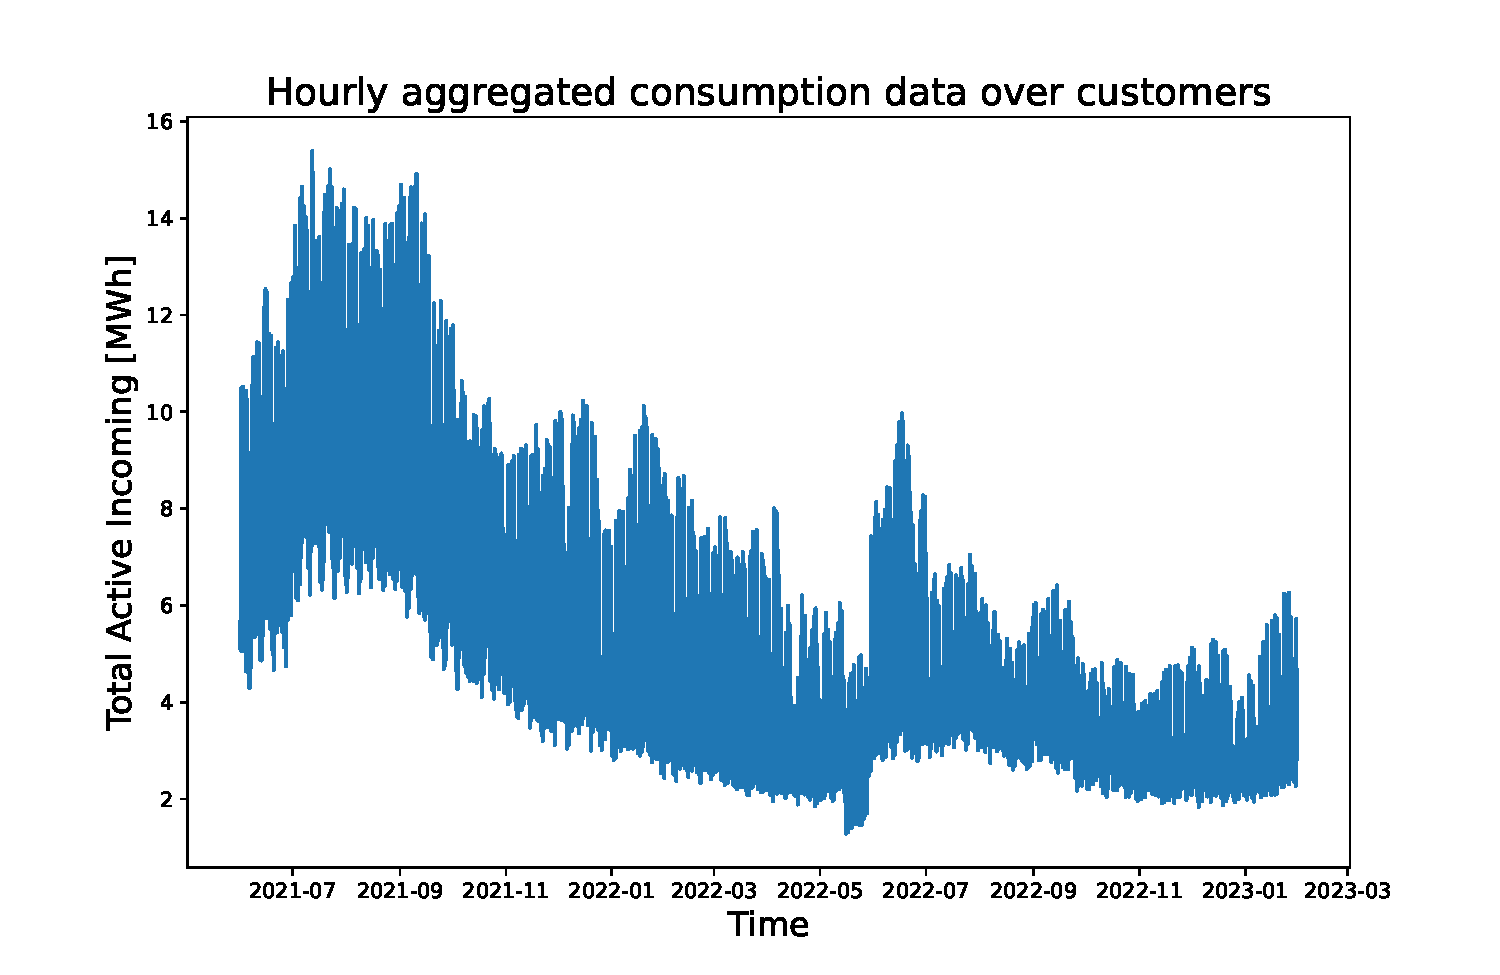
\includegraphics[width=1\textwidth]{images/demand/data_plot}
\subcaption{}
\label{fig:demanddataplot}
\end{minipage}
\ \hspace{2mm} \
\begin{minipage}[b]{8.5cm}
\centering
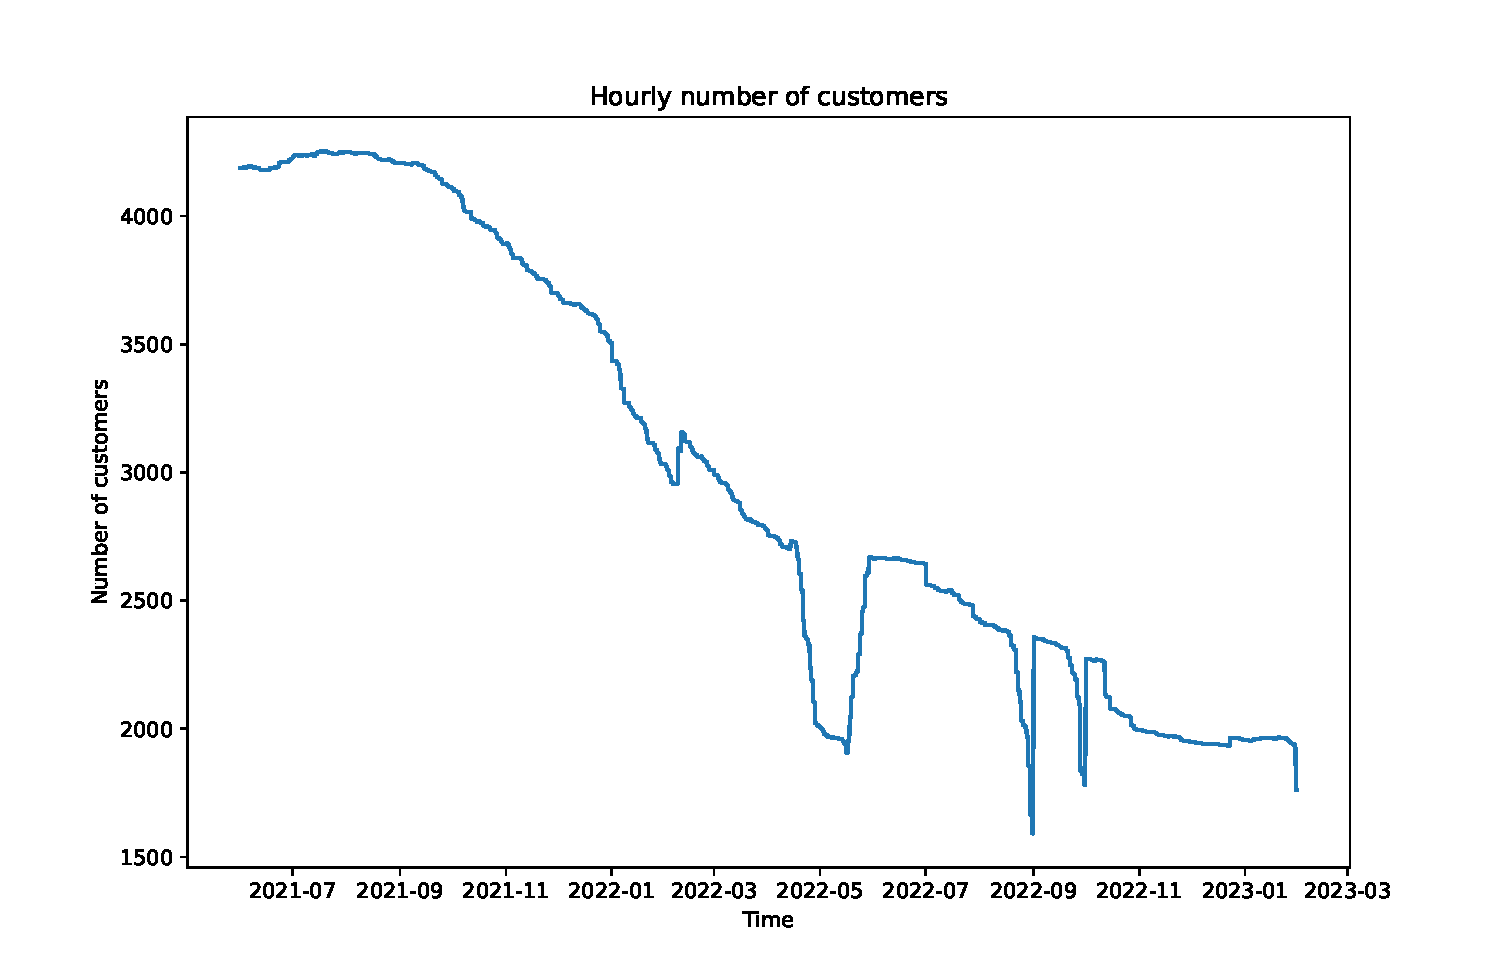
\includegraphics[width=1\textwidth]{images/demand/customers_plot}
\subcaption{}
\label{fig:customersplot}
\end{minipage}
\begin{minipage}[b]{17cm}
\centering
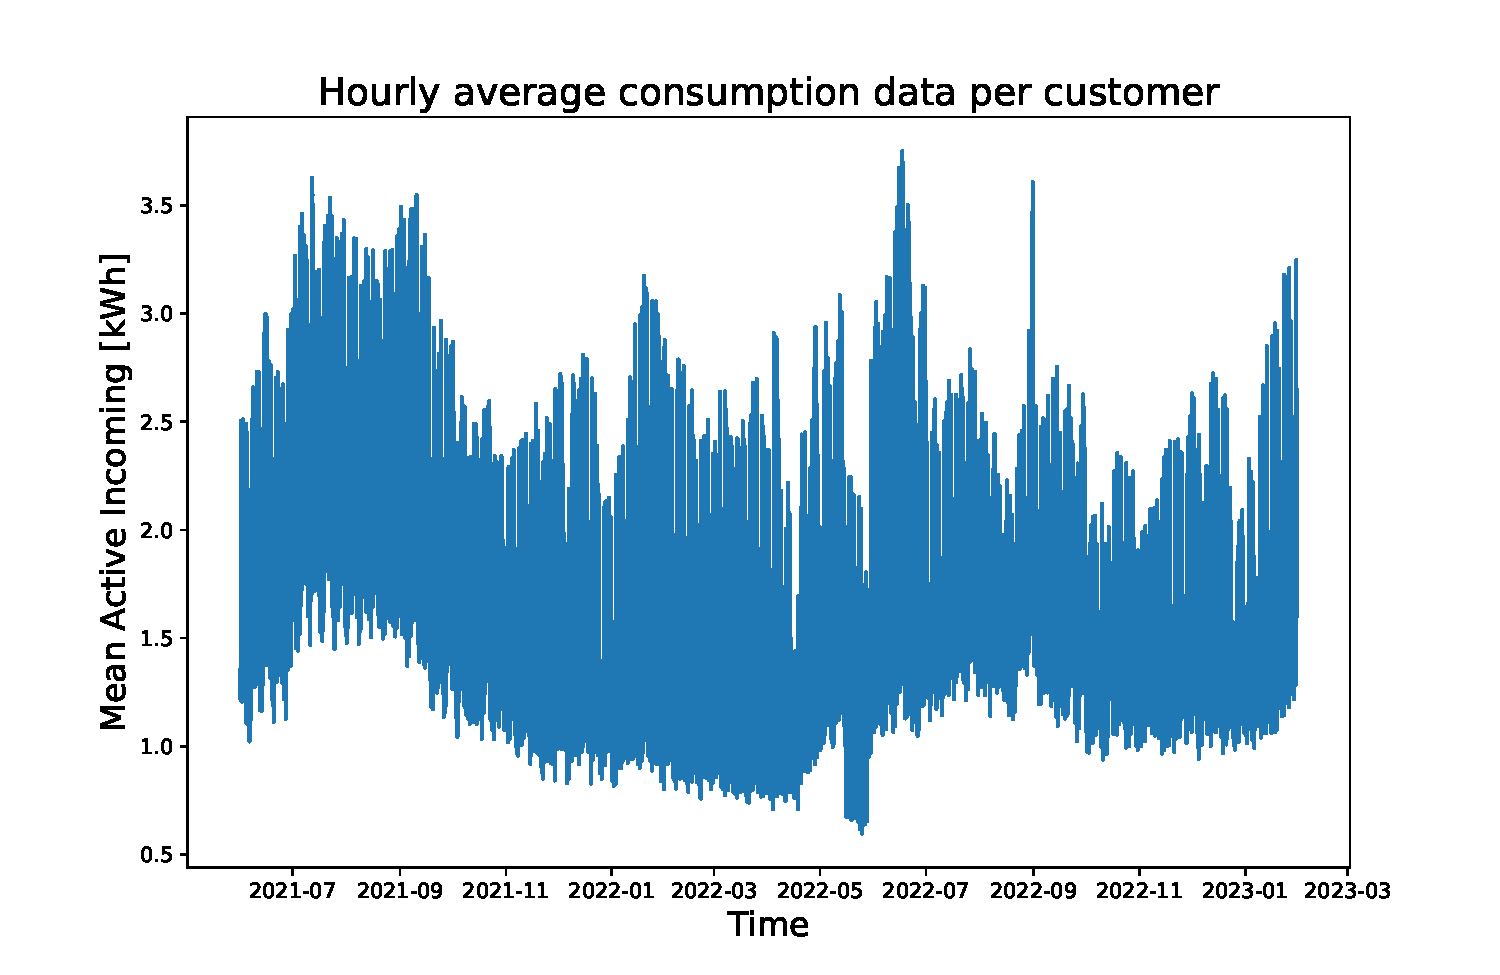
\includegraphics[width=0.5\textwidth]{images/demand/mean_data_plot}
\subcaption{}
\label{fig:meandemanddataplot}
\end{minipage}
\caption{The graphical representation of the hourly \subref{fig:demanddataplot} aggregated consumption data over the customers, \subref{fig:customersplot} number of customers, and \subref{fig:meandemanddataplot} average consumption data per customer.}
\end{figure}

The aggregated consumption data from all their customers consists of hourly aggregated consumption data from June 2021 to January 2023 for a total of 14617 entries.
The graphical representation of the hourly aggregated consumption data is reported in figure~\ref{fig:demanddataplot}.
The number of customers is variable, with a maximum of 4253, a minimum of 1591, a mean of 2988, and a standard deviation of 855.
The graphical representation of the hourly number of customers is reported in figure~\ref{fig:customersplot}.
It was thought to normalize the consumption on the basis of the number of customers in order to study the average consumption data per customer, as illustrated in figure~\ref{fig:meandemanddataplot}, and then multiply by the number of customers.
However, this was not feasible since often this value changes significantly without reflecting on the consumption data, this information was deemed unreliable and not utilized.
Despite this limitation, the average consumption per customer still provided valuable insights into consumption patterns.
Specifically, it suggested the presence of two consumption peaks: one in the summer, likely attributed to air conditioning systems, and a second peak in the winter, likely caused by heating systems.

The consumption data from single customers consists of hourly aggregated consumption data of three customers:
\begin{enumerate}
  \item from June 2021 to August 2022 for a total of 10952 total entries and it is represented in figure~\ref{fig:dataplotcustomer1};
  \item from September 2021 to May 2022 for a total of 5855 total entries and it is represented in figure~\ref{fig:dataplotcustomer2};
  \item from September 2021 to August 2022 for a total of 8760 total entries and it is represented in figure~\ref{fig:dataplotcustomer3}.
\end{enumerate}
The total entries for the three customers are 25567 in the overall period from June 2021 to August 2022.

\begin{figure}[H]
\begin{minipage}[b]{8.5cm}
\centering
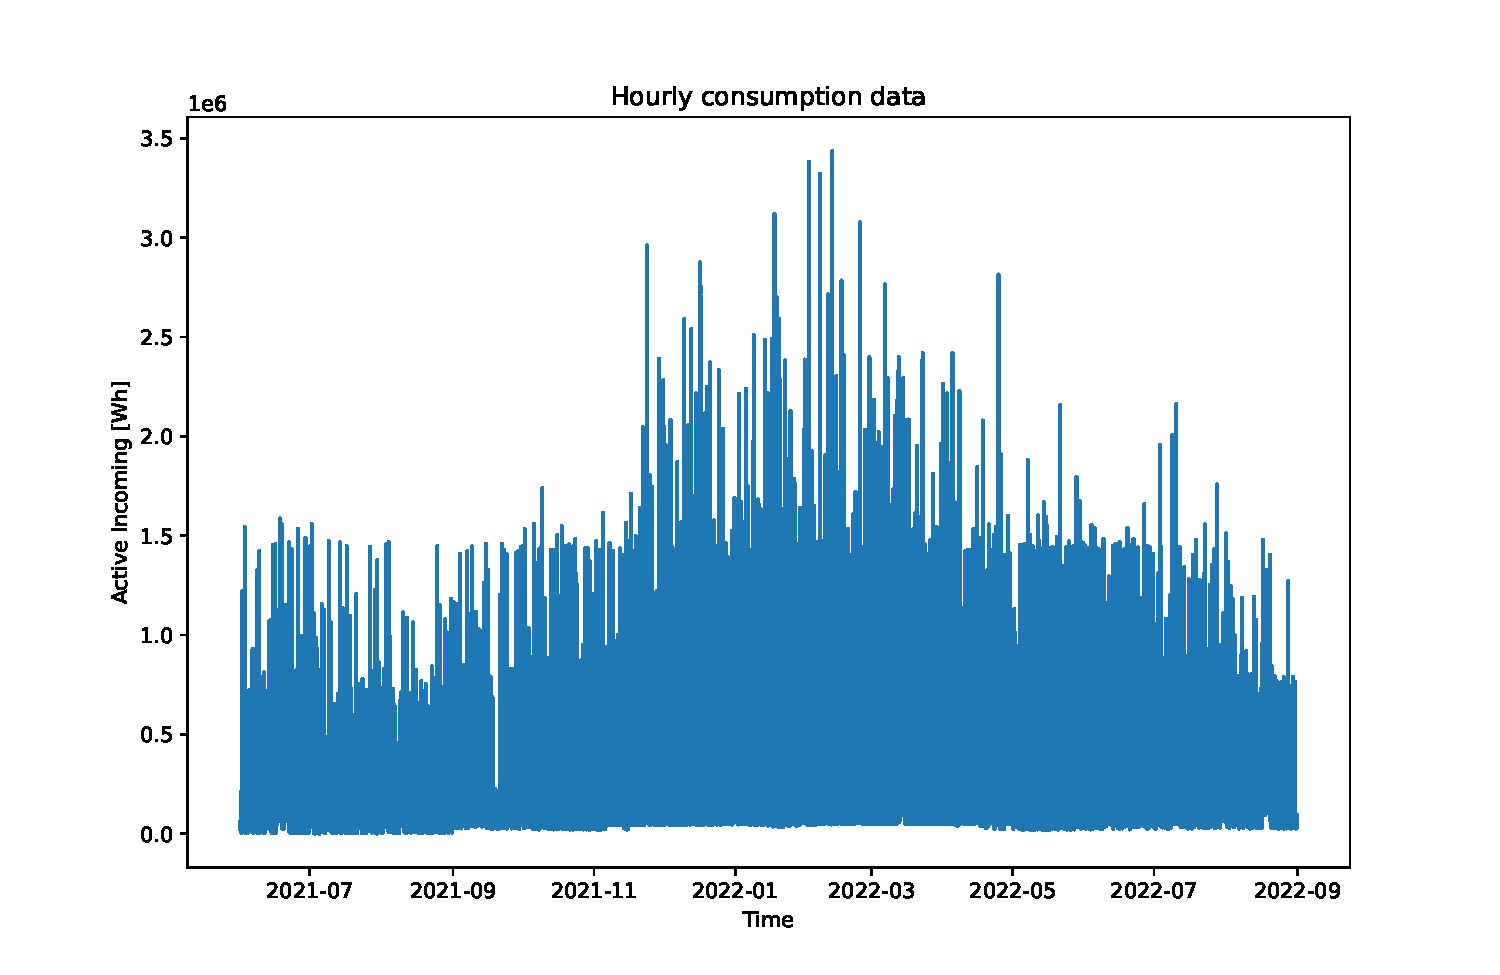
\includegraphics[width=1\textwidth]{images/baseline/data_plot_customer1}
\subcaption{First customer.}
\label{fig:dataplotcustomer1}
\end{minipage}
\ \hspace{2mm} \
\begin{minipage}[b]{8.5cm}
\centering
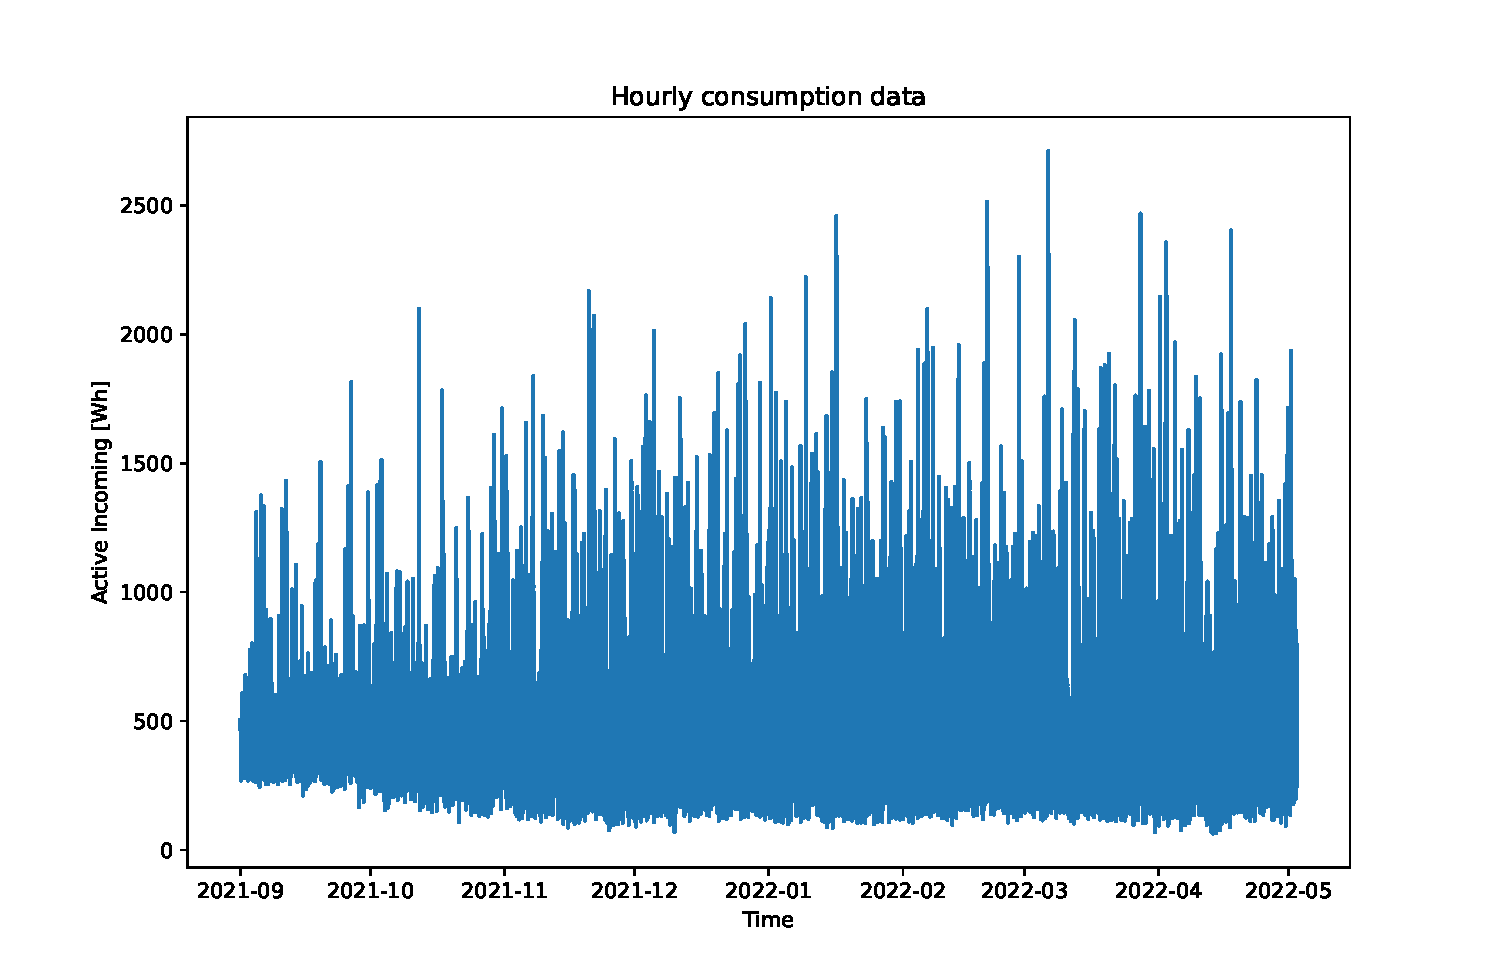
\includegraphics[width=1\textwidth]{images/baseline/data_plot_customer2}
\subcaption{Second customer.}
\label{fig:dataplotcustomer2}
\end{minipage}
\begin{minipage}[b]{17cm}
\centering
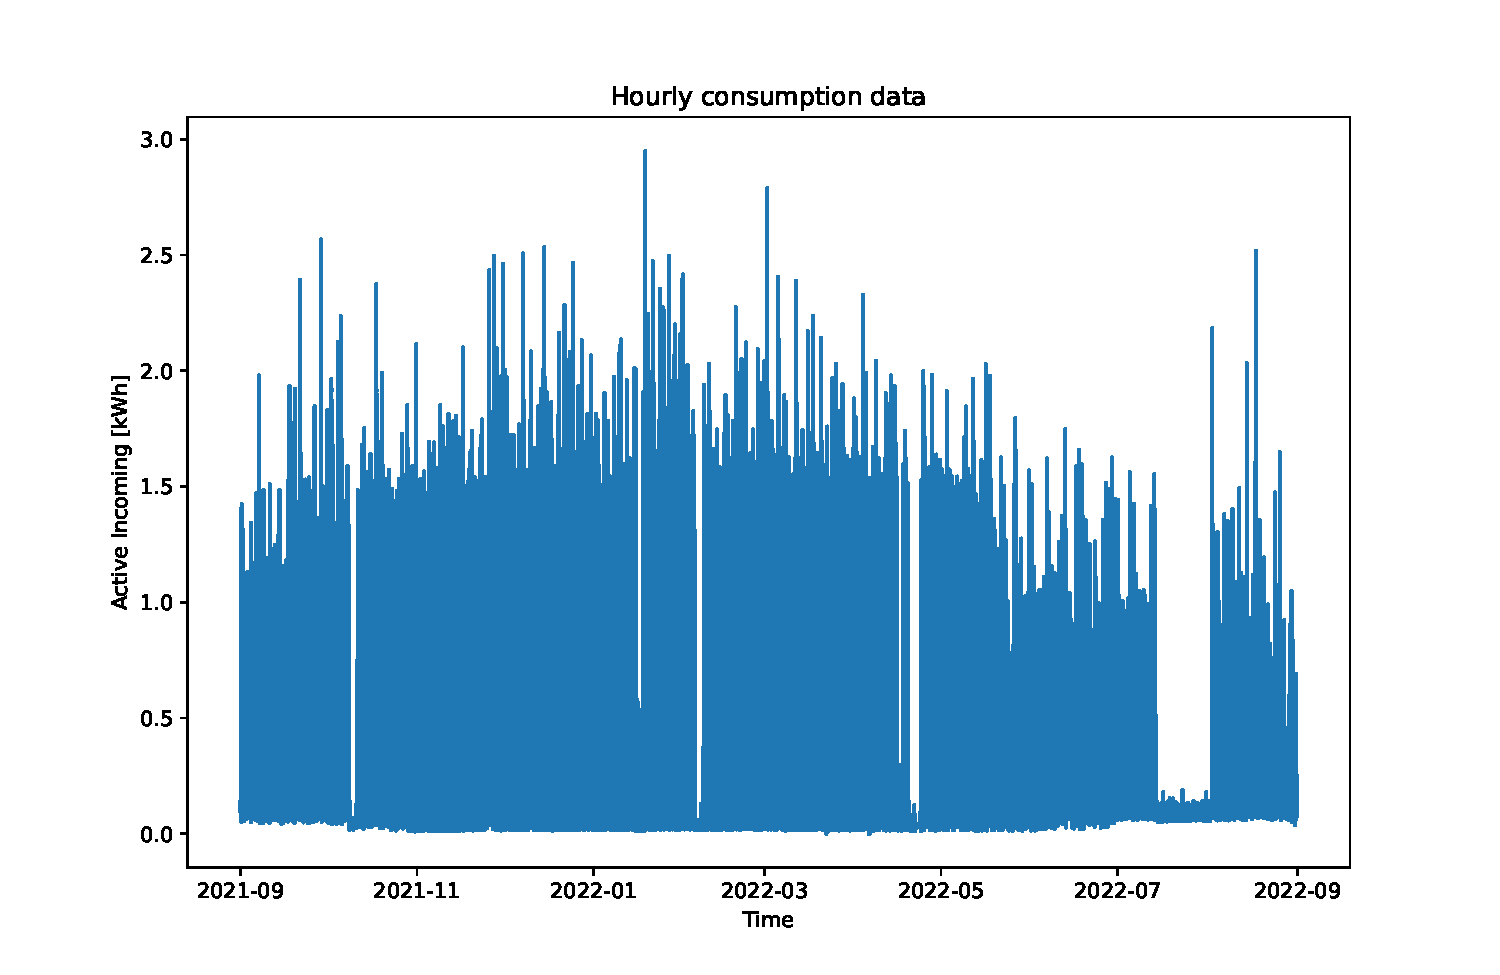
\includegraphics[width=0.5\textwidth]{images/baseline/data_plot_customer3}
\subcaption{Third customer.}
\label{fig:dataplotcustomer3}
\end{minipage}
\caption{The graphical representation of the consumption data of the three customers.}
\end{figure}

Only consumption data for three customers were provided, as electricity consumption data of customers is considered personal data as stated in the Directive (EU) 2019/944 of the European Parliament\footnote{ \url{https://eur-lex.europa.eu/legal-content/EN/TXT/?uri=CELEX:32019L0944} }, which establishes common rules for the internal market for electricity.
As such, the data falls under the scope of the General Data Protection Regulation (GDPR)\footnote{ \url{https://gdpr-info.eu/} }, which requires explicit consent for processing personal data.
Therefore, it is likely that the provided data came from MIWenergía's internal employees who consented to participate in the research.
In fact, the provided data were needed for a technical feasibility study.
However, to identify consumption patterns among a broader population, data from more customers would be required.

By analyzing the data plots, it can be observed that the consumption patterns of the three customers are quite distinct.
For instance:
\begin{itemize}
  \item The first customer's consumption is consistently below 1.5 kWh throughout the year except for the winter season;
  \item The second customer shows almost the same consumption pattern;
  \item The third customer has a dense series with some gaps with very low consumption in parts of the year, probably due to time periods away from home.
\end{itemize}

The production data from 8 PV plants consists of hourly aggregated production data:
\begin{enumerate}
  \item from January 2022 to October 2022 for a total of 7296 total entries and it has a nominal power of 149.75 kW;
  \item from February 2022 to October 2022 for a total of 6552 total entries and it has a nominal power of 237.6 kW;
  \item from February 2022 to October 2022 for a total of 6552 total entries and it has a nominal power of 158.4 kW;
  \item from June 2022 to October 2022 for a total of 3576 total entries and it has a nominal power of 1240 kW;
  \item from September 2022 to October 2022 for a total of 1465 total entries and it has a nominal power of 126.2 kW;
  \item from September 2022 to October 2022 for a total of 1465 total entries and it has a nominal power of 113 kW;
  \item from September 2022 to October 2022 for a total of 1465 total entries and it has a nominal power of 45 kW;
  \item from September 2022 to October 2022 for a total of 1465 total entries and it has a nominal power of 100 kW;
\end{enumerate}
The total entries for the 8 PV plants are 29836 total entries in the overall period from January 2022 to October 2022, aggregating over plants the resulting entries are 7296.
The graphical representation of the hourly aggregated total production data and mean percentage of production data are reported respectively in figure~\ref{fig:productiondataplot} and figure~\ref{fig:productiondataplotpercentage}.

The same weather data from the same provider and the same weather station were used for all the tasks.
While it is reasonable to assume that some weather conditions, such as clouds, may vary and affect consumption and production differently, this approach was taken since the customers and the PV plants were in the same area, with a maximum distance of around 100 km between them, and also because the value of the weather parameters is an average of the values recorded in the past hour.
Therefore, using the same weather data is deemed appropriate for the analysis at hand, given that it reflects the weather conditions in the area over a broad time frame.

\begin{figure}[H]
\begin{minipage}[b]{8.5cm}
\centering
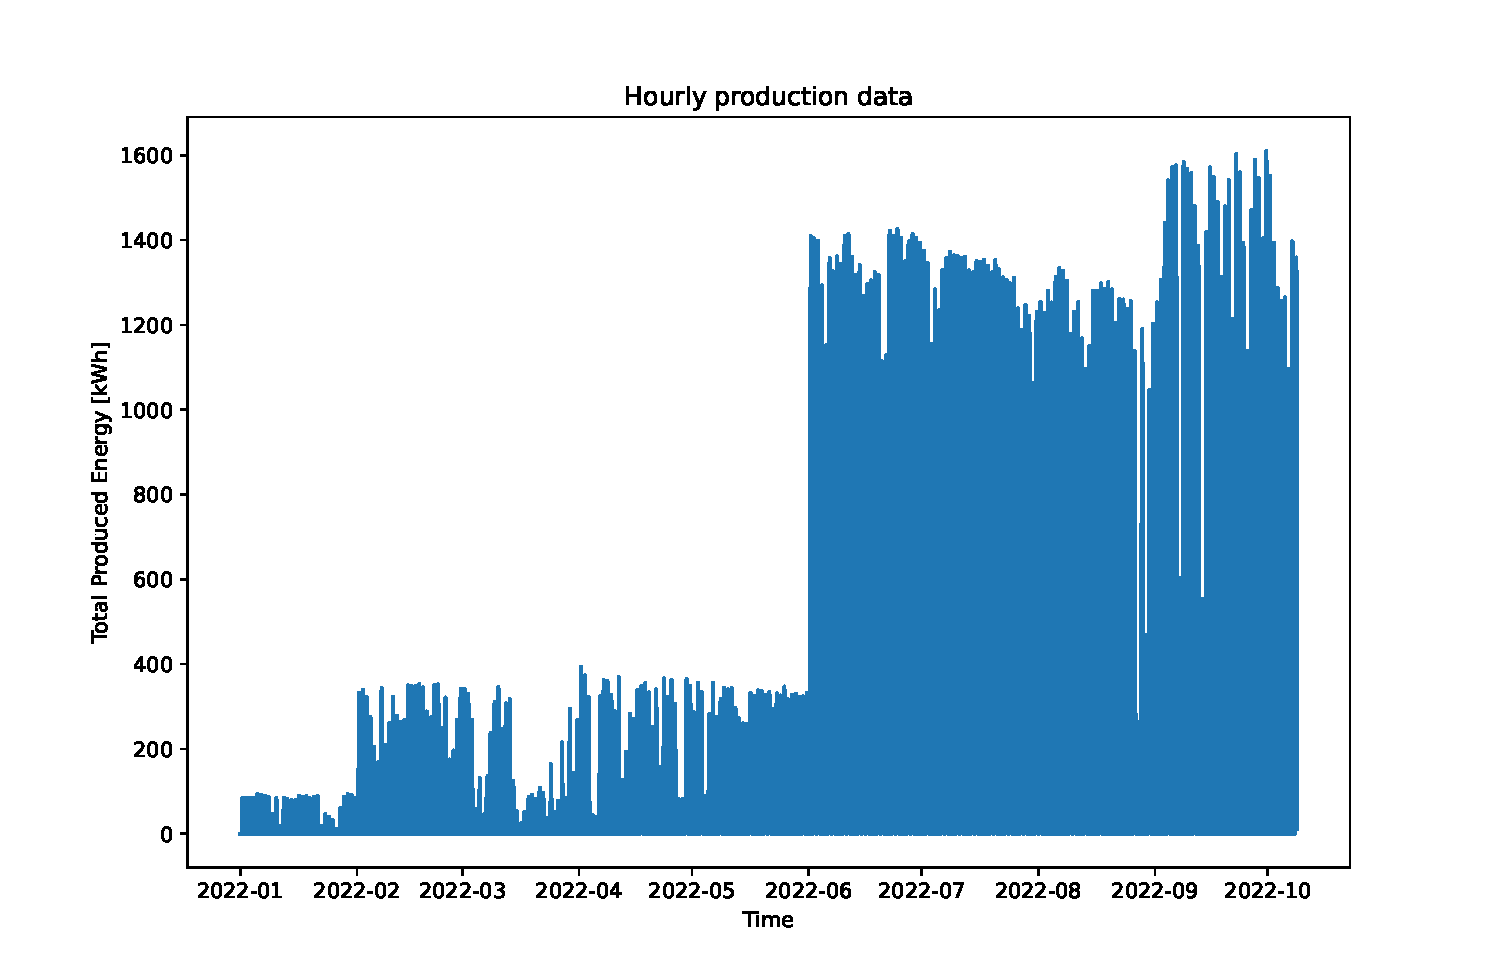
\includegraphics[width=1\textwidth]{images/production/data_plot}
\subcaption{}
\label{fig:productiondataplot}
\end{minipage}
\ \hspace{2mm} \
\begin{minipage}[b]{8.5cm}
\centering
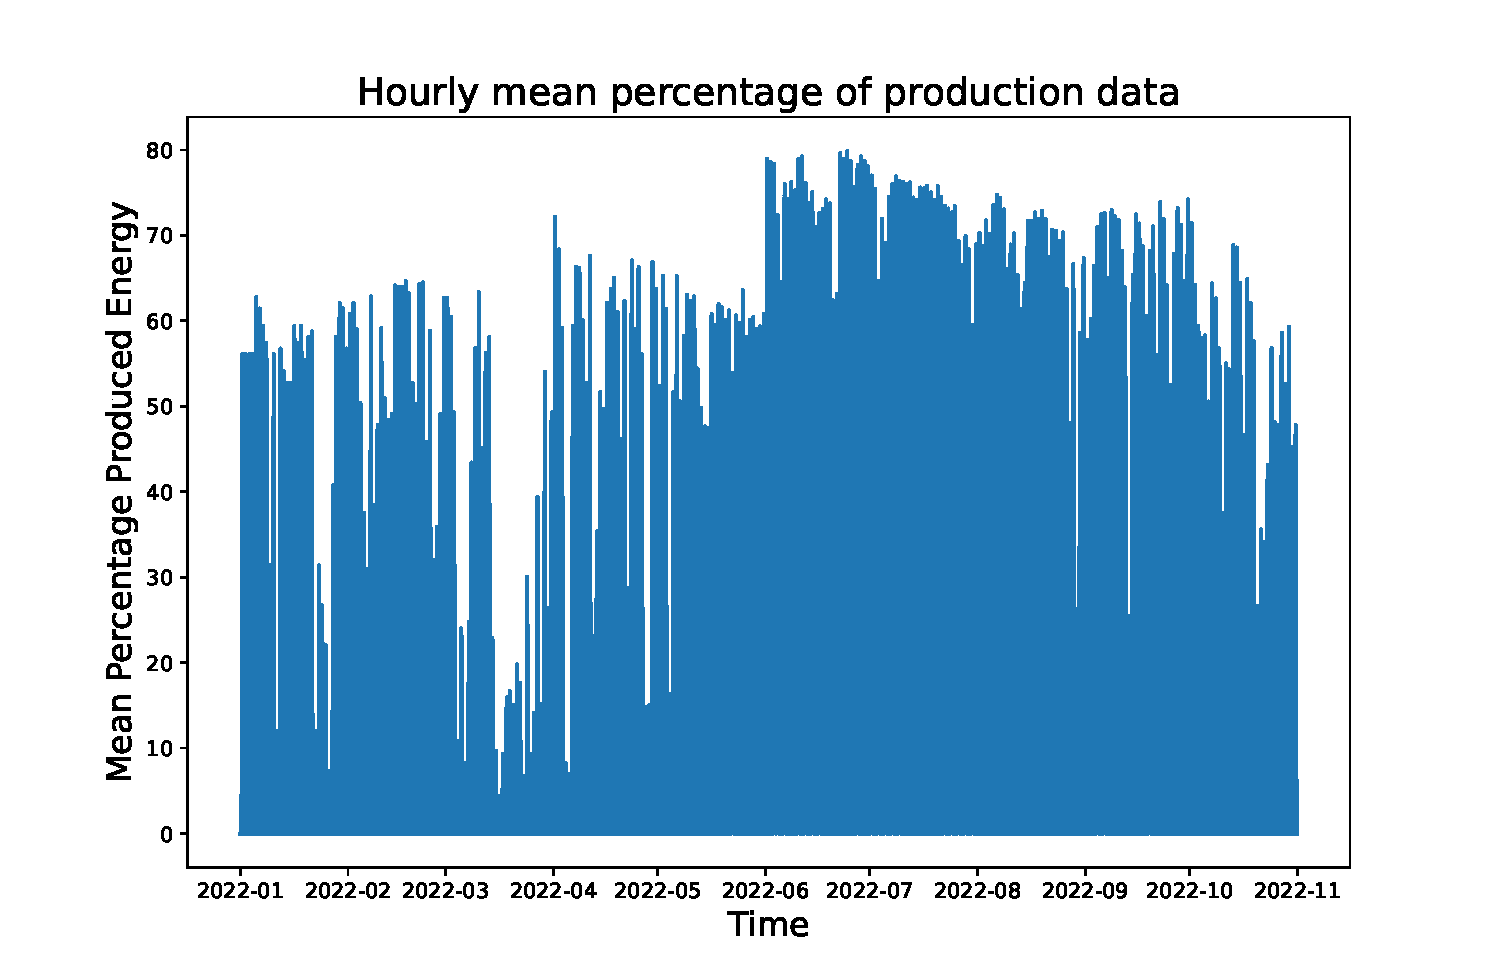
\includegraphics[width=1\textwidth]{images/production/data_plot_percentage}
\subcaption{}
\label{fig:productiondataplotpercentage}
\end{minipage}
\caption{The graphical representation of the hourly aggregated \subref{fig:productiondataplot} total production data and \subref{fig:productiondataplotpercentage} mean percentage of production data.}
\end{figure}


\section{Evaluation methodology}
\label{sec:methodology}
\vspace{0.2 cm}

The evaluation methodology was based on two relevant error metrics: MAPE and MAE.
These are standard and widely used metrics in time series forecasting for different use cases, as reported in many articles and books such as \cite{armstrong2001principles, DEGOOIJER2006443, HYNDMAN2006679}.
The MAPE is defined as $\text{MAPE}(y, \hat{y}) = \frac{100\%}{N} \sum_{i=0}^{N - 1} \frac{|y_i - \hat{y}_i|}{|y_i|}$.
It is the most relevant error metric for all the tasks since it is a percentage-based error metric that takes into account the magnitude of the errors relative to the actual values.
The MAE is defined as $\text{MAE}(y, \hat{y}) = \frac{ \sum_{i=0}^{N - 1} |y_i - \hat{y}_i| }{N}$.
It is the most suitable error metric in consumption baseline forecasting where there is a high variability from very low to high values, and electricity production forecasting where there is a significant number of zeros when the sun is absent.

\begin{figure}[H]
\centering
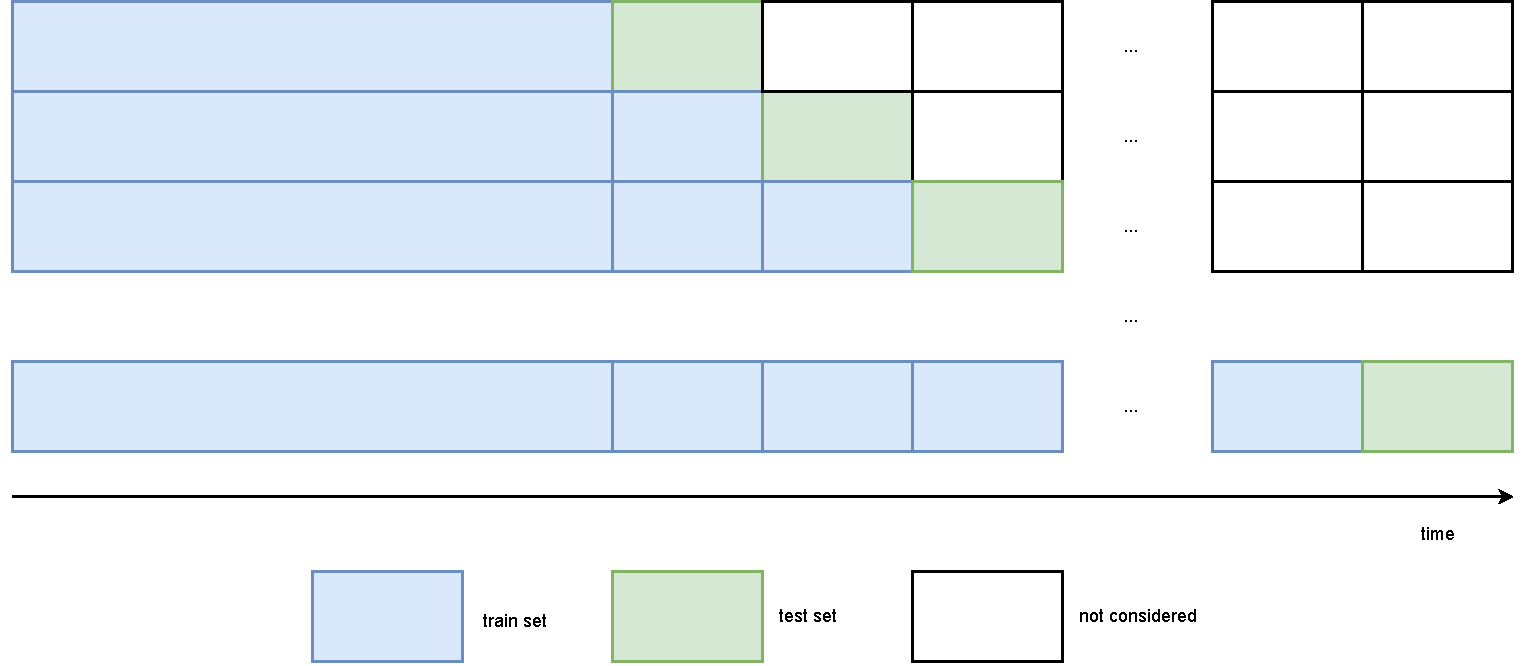
\includegraphics[width=0.8\textwidth]{images/cross_validation}
\caption{The schematic representation of the blocked k-fold cross-validation adopted.}
\label{fig:crossvalidation}
\end{figure}

For assessing the model performance when dealing with time series data, the traditional cross-validation techniques are not suitable as they assume that the data points are independent and identically distributed (i.i.d.), which is not the case in time series data, as also reported in the Chapter~\ref{cha:soa} by the following articles \cite{BERGMEIR2012192, Cerqueira2020}.
In fact, in time series data the order of the observations matters, and there are temporal dependencies between the observations.
Therefore, a more appropriate technique for evaluating time series models is blocked k-fold cross-validation.
The basic idea of blocked k-fold cross-validation is to split the data considering multiple training and test sets, where the training set only includes data from the past and the test set includes data from the future.
This simulates the real-world scenario where we want to make predictions about the future based on past data.
In figure~\ref{fig:crossvalidation}, the schematic representation of how the blocked k-fold cross-validation was performed is reported, 12 splits were used with a test size depending on the specific use case.
The training set is increased by adding the previous test elements at every successive evaluation.

Another technique, reported in \cite{Cerqueira2020} is the repeated holdout approach repeated in multiple testing periods using a Monte Carlo simulation.
This approach involved using 70\% of the total observations of the time series in each test.
For each period, a random point from the time series was selected, and a training window comprising 60\% of the time series before the selected point was used for training, while a testing window of 10\% of the time series after the selected point was used for evaluation.
In the paper, it was stated that the approach provided the most accurate estimates when the time series are non-stationary.
However, for having the same evaluation mechanisms on all the models and simulating the fact that the model starts with limited data and then the training amount increases over time to obtain better performance, block validation was used using the TimeSeriesSplit provided by the scikit-learn library.
Moreover, the considered data are without a strong trend as reported in the dedicated sections of the specific use cases where the data and the model forecasts are analyzed.

In addition to the blocked k-fold cross-validation results also the results on the last test split using the rest as training are reported.
This was done since it provides insight on which could be the performance of the models in forecasting the near future data with the currently available training data.
A table summarizing the metrics and the evaluation mechanisms adopted for the use cases is reported in table~\ref{tab:metricstable}.

\begin{table}[H]
\centering
\begin{tabular}{|c|c|c|}
\hline
\textbf{Use case} & \textbf{Metrics} & \textbf{Evaluation mechanisms}\\
\hline
Electricity demand & MAPE & blocked k-fold cross-validation\\
forecasting & & and test on the last split\\
\hline
Electricity production & MAE & blocked k-fold cross-validation\\
forecasting & & and test on the last split\\
\hline
Consumption baseline & MAPE and MAE & blocked k-fold cross-validation\\
forecasting & & and test on the last split\\
\hline
\end{tabular}
\caption{Table summarizing the metrics and the evaluation mechanisms adopted for the use cases.}
\label{tab:metricstable}
\end{table}

This evaluation methodology was used at training time to study the performance over time.
At forecasting time, the performance on the last time slot was treated with more attention as the most relevant for the electricity retailers since the most related to the performance on imminent future data.
The combinations of the models were done just at forecasting time on the last time slot using the average of some approaches for studying whether there could be a beneficial effect on the forecasts and compensation of error between the different approaches.
The same was also done for the AutoML approach, in fact, it was tested just at forecasting time on the last time slot for comparison to the tested models.
It was included as a baseline to show how a general-purpose framework can perform in specific use cases compared to specific architectures designed for the task.

As explained in Chapter~\ref{cha:implementation}, for all the use cases, there is a difference between training and forecasting time for the ML (support vector regressor, hist gradient boosting regressor, and extreme gradient boosting regressor) and DL (LSTM, GRU, and CNN) models.
In particular, for these models, a recursive strategy to generate multi-step forecasts was adopted.
This approach is a standard classical technique covered in various textbooks, including \cite{Manu2022}.
It offers advantages such as simplicity in understanding, clear temporal dependency as previous forecasts are used as input for subsequent ones, flexibility to be applied to different models, and adaptability to various forecasting horizons, which is crucial when integrating it into a SaaS solution.
However, there are also disadvantages associated with this approach.
Error propagation can occur, and this can be observed in the forecasting results, where small inaccuracies in initial predictions can accumulate and lead to larger errors over time.
Sub-optimality is another drawback, as the optimality achieved for one-step forecasting may not generalize well to multi-step forecasting.
Additionally, the computational complexity is high as the model needs to be run for each individual step.
In contrast, the other approaches: baselines, ARIMA/SARIMA, Prophet, and TFT directly handle the concept of multi-step prediction and present no difference between training and forecasting time.


\section{Electricity demand forecasting}
\label{sec:demandval}
\vspace{0.2 cm}

The aggregated consumption data over the customers is analyzed to get some descriptive analytics before finding adequate models to forecast the demand.

The time series decomposition using an additive model of the hourly aggregated consumption data over the customers considering as period of the time series a week is reported in figure~\ref{fig:demanddecomposition}.
It showed a considerable amount of noise, comparable to seasonality in magnitude.
The trend showed 2 peaks during the summer season, the first being more emphasized since it also corresponds to a peak in the number of users.

\begin{figure}[H]
\centering
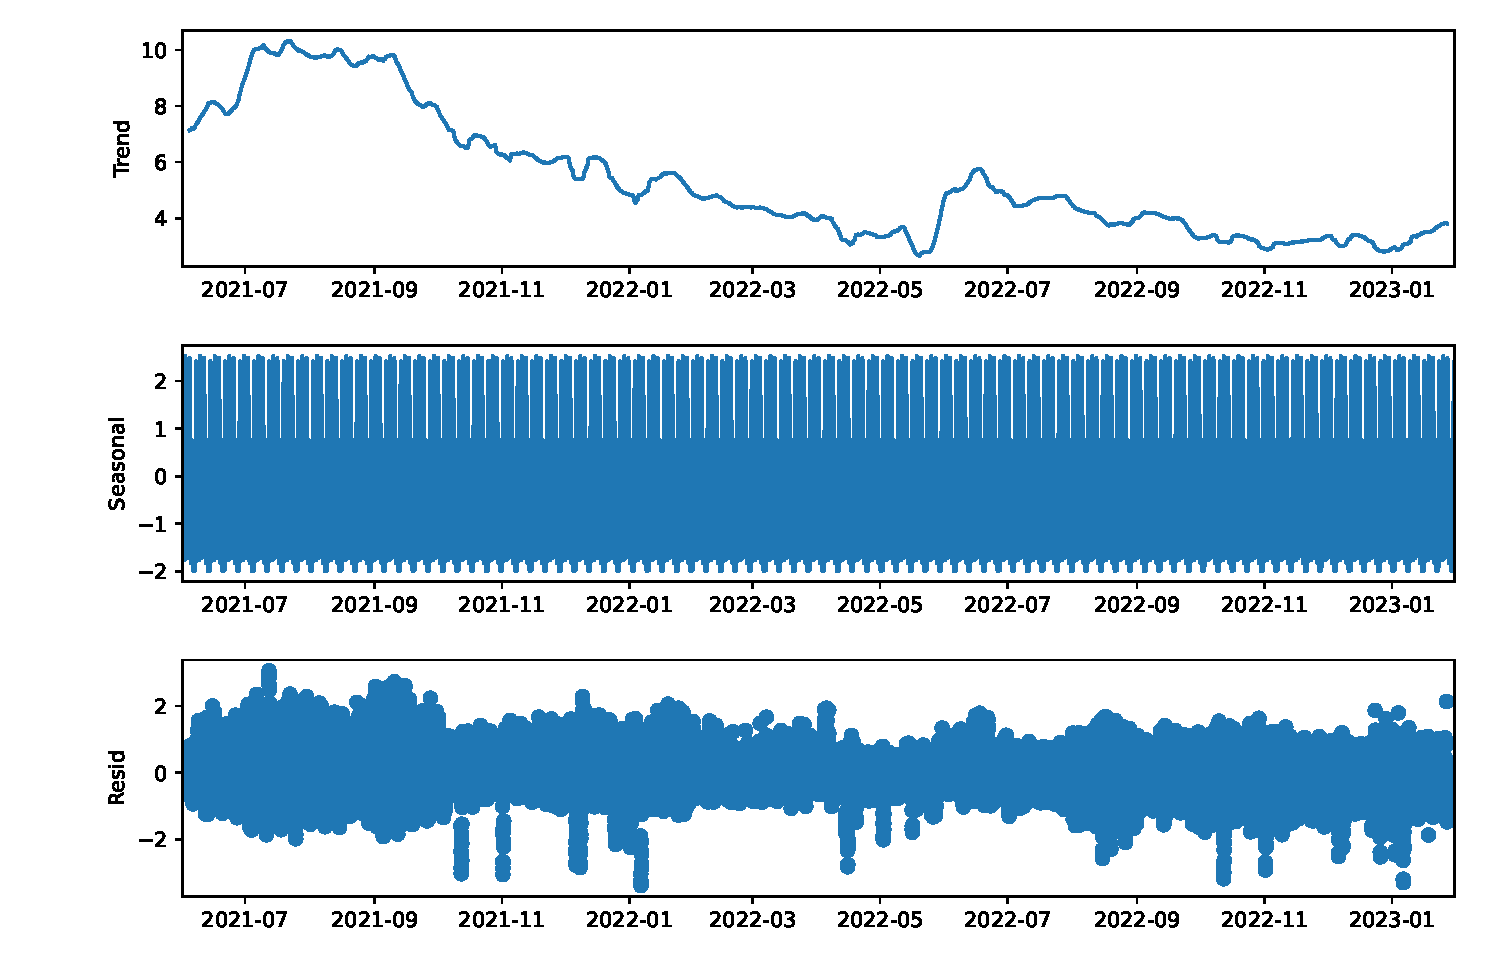
\includegraphics[width=0.475\textwidth]{images/demand/hourly_decomposition_week_period}
\caption{The time series decomposition of the hourly aggregated consumption data over the customers considering as period of the time series a week.}
\label{fig:demanddecomposition}
\end{figure}

The auto-correlation of the hourly aggregated consumption data over the customers is reported in figure~\ref{fig:demandcorrelation}.
It shows a high auto-correlation value in the close time lags and also at every 24 hours, along with an even higher value at a one-week distance.
This indicates that the consumption data from the closest time lags, particularly up to three closest ones, as well as those corresponding to the same hour in the preceding days and even better in the preceding weeks, may be valuable features for predicting a time instant's demand.
A reasonable balance can be achieved by incorporating the consumption data from the past 14 days.

\begin{figure}[H]
\centering
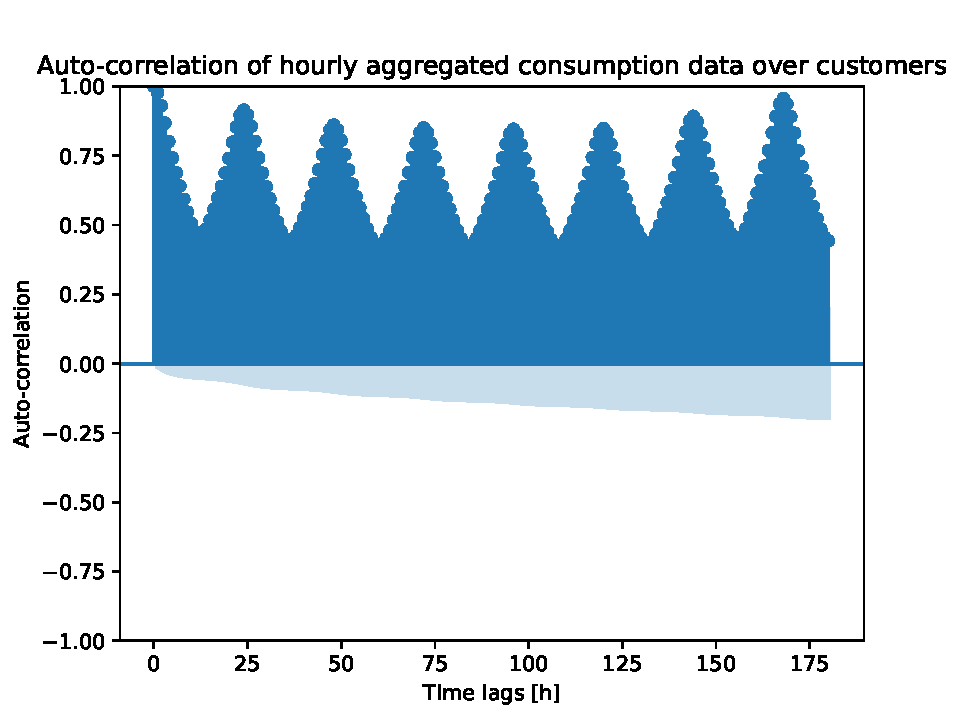
\includegraphics[width=0.4\textwidth]{images/demand/hourly_correlation_week_range}
\caption{The auto-correlation of the hourly aggregated consumption data over the customers.}
\label{fig:demandcorrelation}
\end{figure}

The coefficients given by the Fourier transform for the hourly aggregated consumption data over the customers are reported in figure~\ref{fig:demandft}.
The graphical representation shows 2 main frequencies, one representing the weekly periodicity and one the daily periodicity.
Other minor peaks are present mostly at multiples of the 1/week frequency.

\begin{figure}[H]
\centering
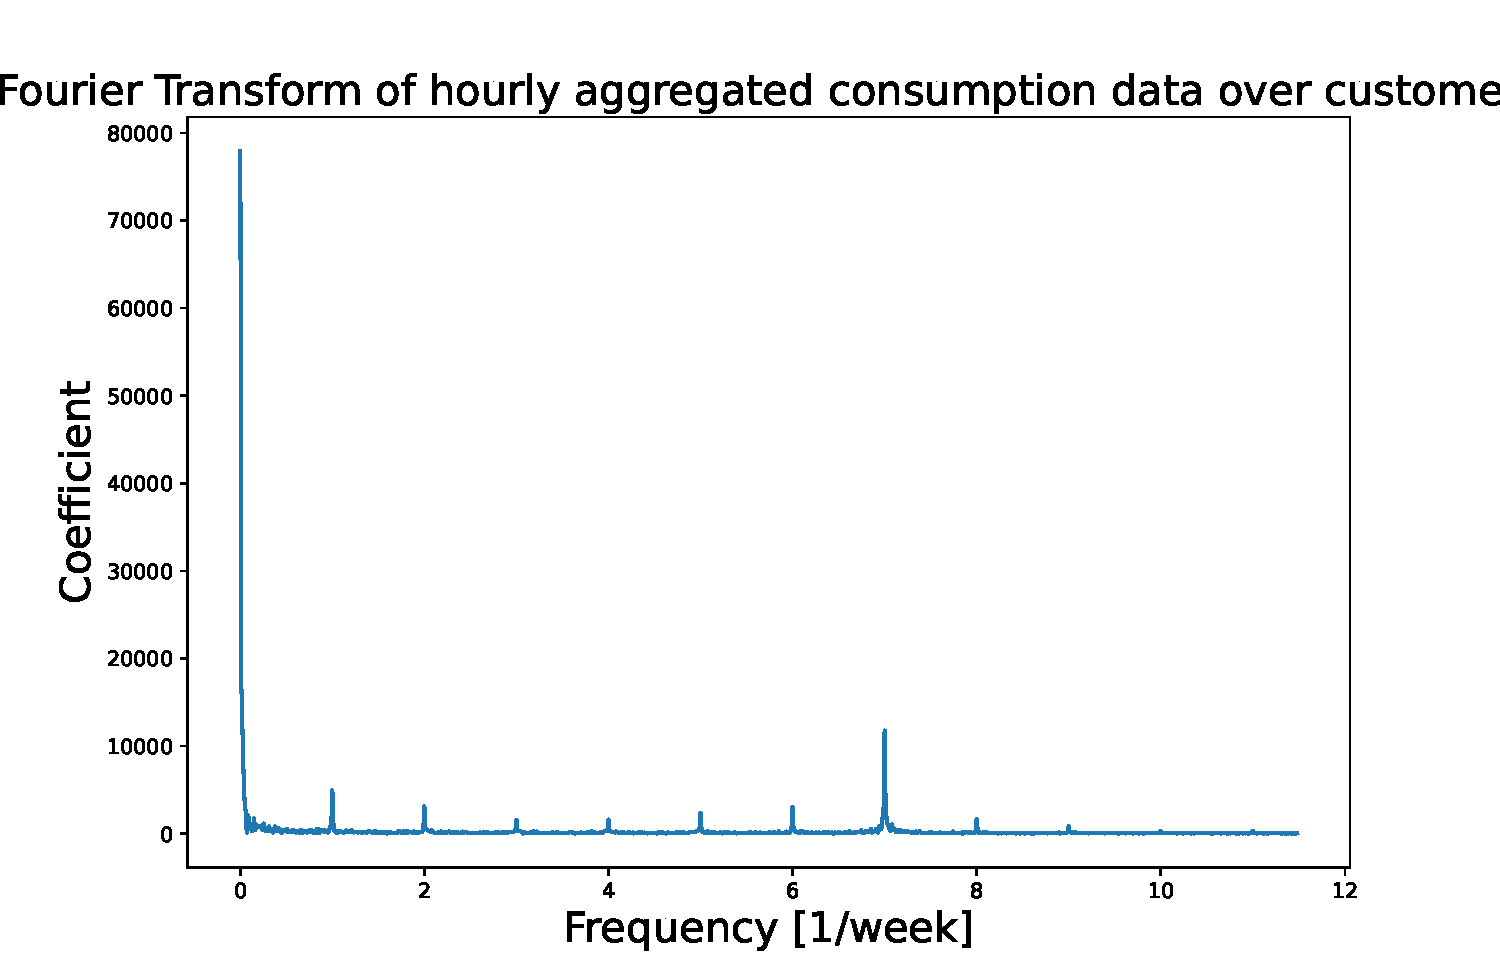
\includegraphics[width=0.4\textwidth]{images/demand/ft_hour_week}
\caption{The coefficients given by the Fourier transform for the hourly aggregated consumption data over the customers.}
\label{fig:demandft}
\end{figure}

The daily aggregated consumption data over the customers is reported in figure~\ref{fig:demanddataplotday}.
Aggregating the data on a daily basis, it is possible to more clearly observe the weekly pattern of consumption, which exhibits an increase on weekdays and a decrease on weekends.

\begin{figure}[H]
\centering
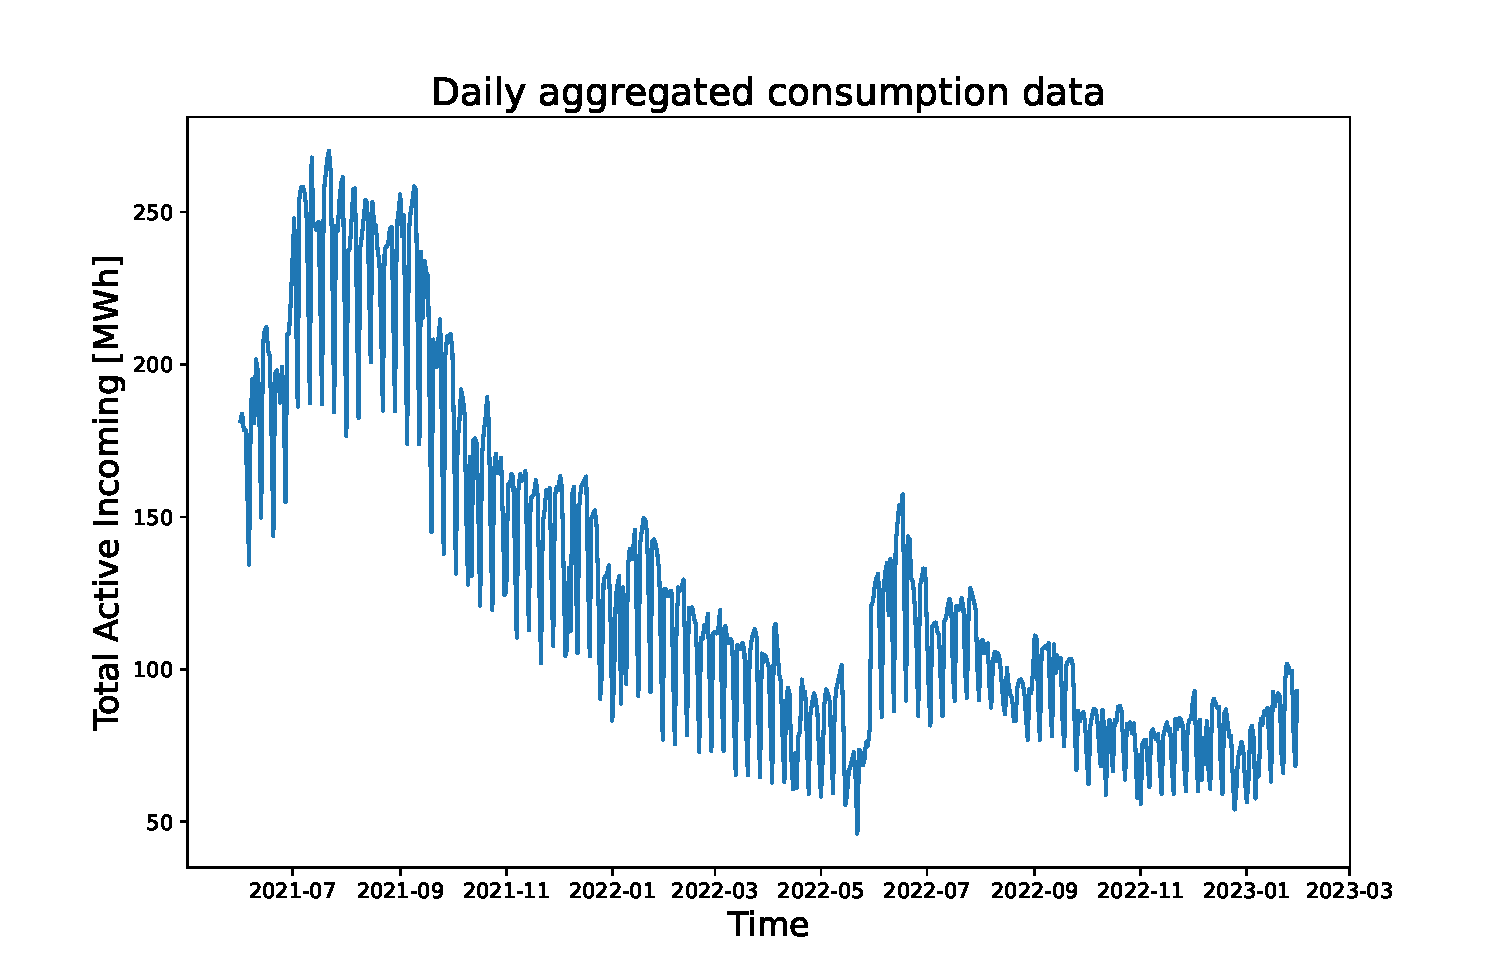
\includegraphics[width=0.5\textwidth]{images/demand/data_day_aggregated_plot}
\caption{The daily aggregated consumption data over the customers.}
\label{fig:demanddataplotday}
\end{figure}

Figure~\ref{fig:demanddecompositionday} shows the time series decomposition of the daily aggregated consumption data over the customers, using an additive model with a period of one week.
The decomposition is consistent with the hourly aggregated consumption over the customers.

\begin{figure}[H]
\centering
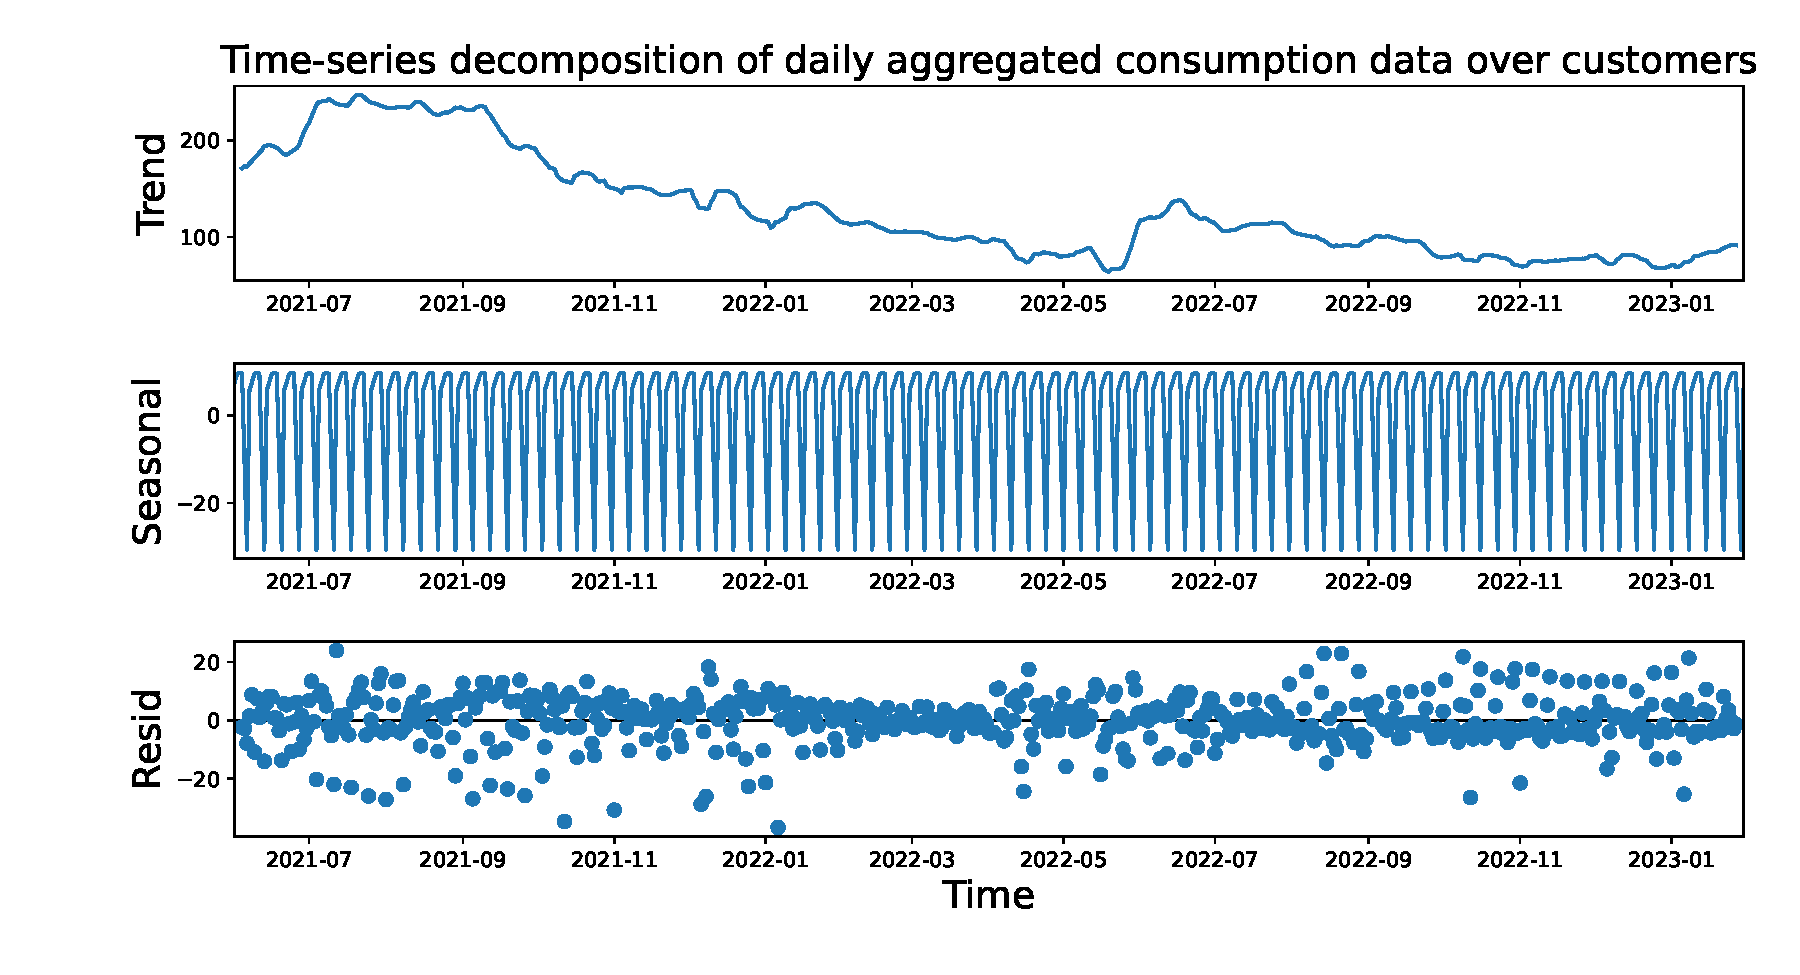
\includegraphics[width=0.475\textwidth]{images/demand/daily_aggregated_decomposition}
\caption{The time series decomposition of the daily aggregated consumption data over the customers considering as period of the time series a week.}
\label{fig:demanddecompositionday}
\end{figure}

The auto-correlation of the daily aggregated consumption data over the customers is reported in figure~\ref{fig:demandcorrelationday}.
It shows a high auto-correlation value in the closest time lag, with an even greater value at every week lag.
This suggests that useful features, since highly correlated, for predicting a time instant's demand may be the closest ones, but also those from the same day of the week in the previous weeks.
A good trade-off can be achieved by considering the consumption data in the previous 14 days.

\begin{figure}[H]
\centering
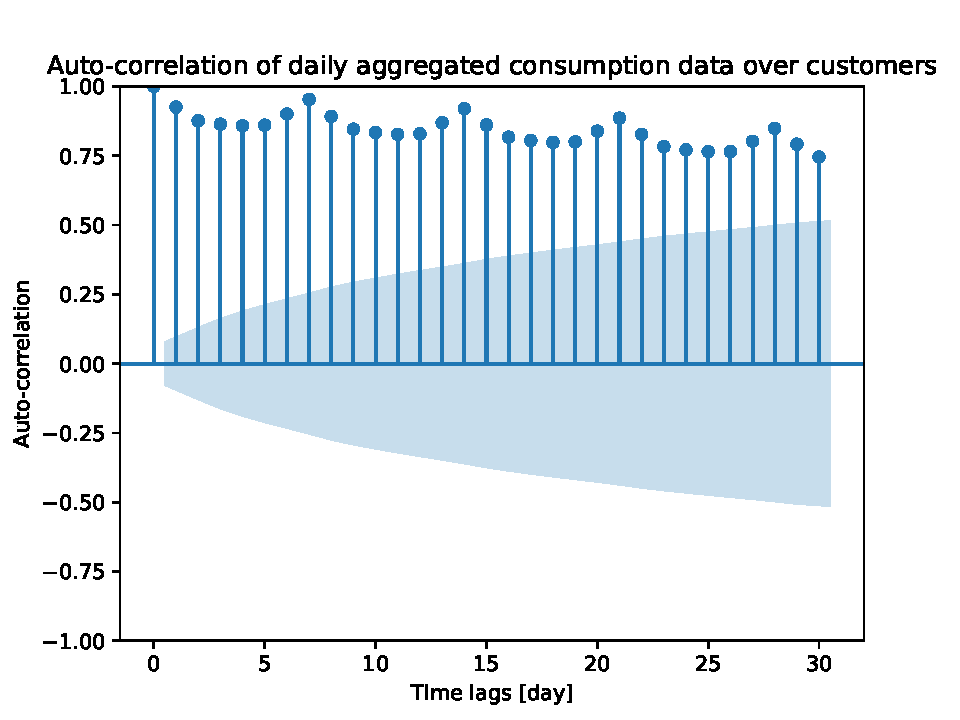
\includegraphics[width=0.4\textwidth]{images/demand/daily_aggregated_correlation}
\caption{The auto-correlation of the daily aggregated consumption data over the customers.}
\label{fig:demandcorrelationday}
\end{figure}

The coefficients given by the Fourier transform for the daily aggregated consumption data over the customers are reported in figure~\ref{fig:demandftday}.
The graphical representation shows 1 main frequency representing the weekly periodicity and other minor peaks at multiples of the 1/week frequency.

\begin{figure}[H]
\centering
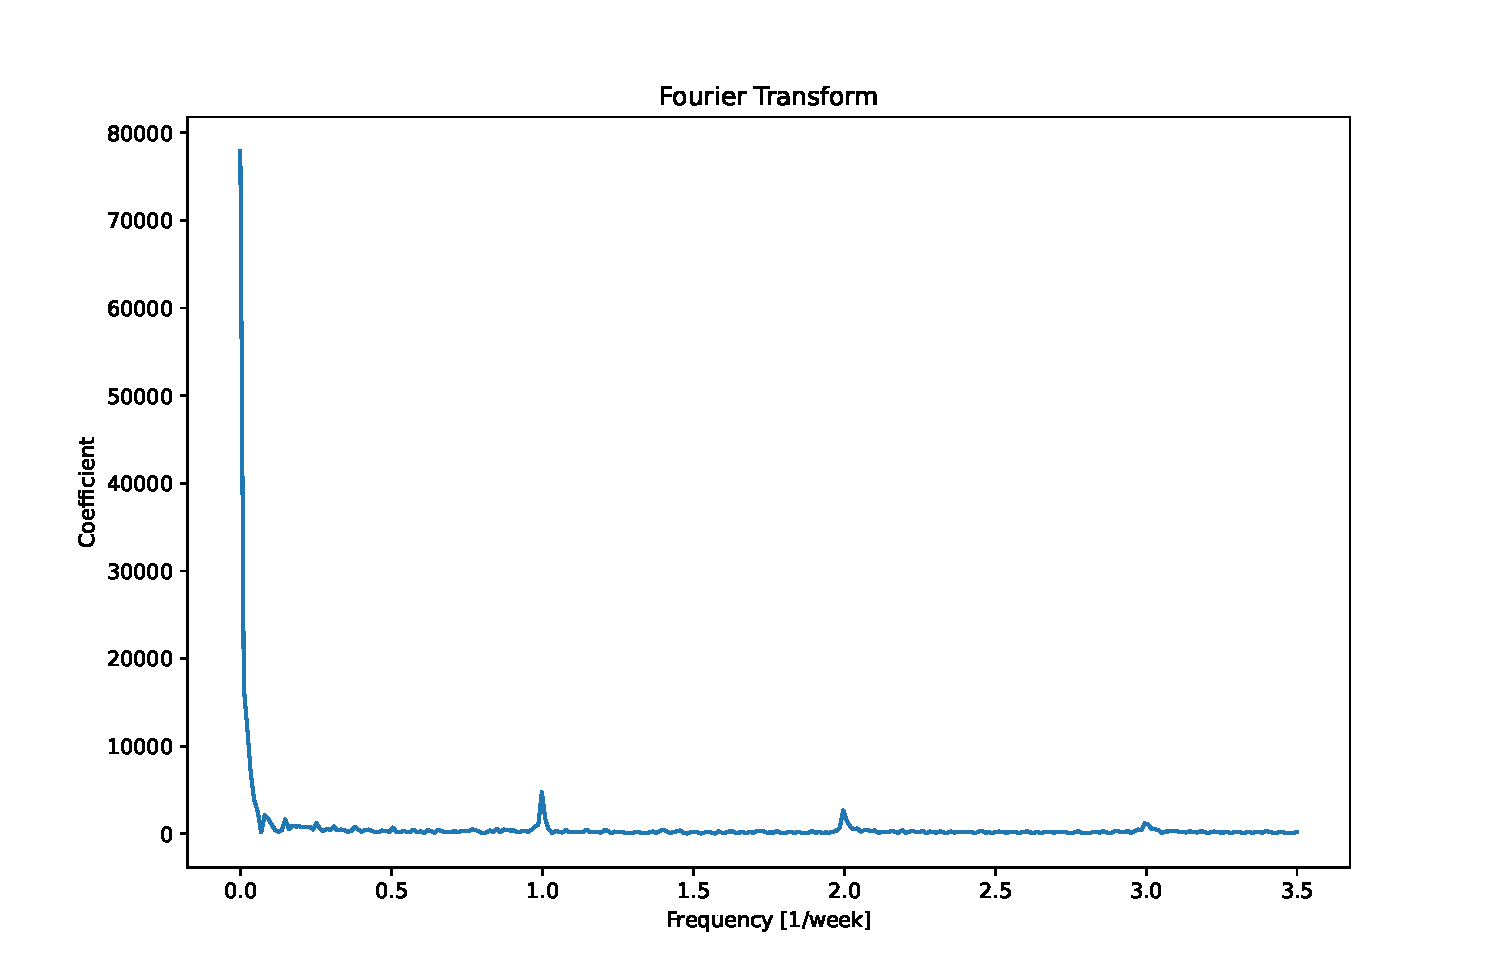
\includegraphics[width=0.4\textwidth]{images/demand/ft_day}
\caption{The coefficients given by the Fourier transform for the daily aggregated consumption data over the customers.}
\label{fig:demandftday}
\end{figure}

Basic data is enhanced with the air temperature, the apparent temperature, and the relative humidity since they are considered the only weather features capable of influencing customers' electricity consumption.
To assess the relationship between these weather variables and the aggregated consumption over the customers, two correlation coefficients were used: Pearson's correlation coefficient and Spearman's rank correlation coefficient.
Pearson's correlation coefficient measures the strength of the linear relationship between two variables, while Spearman's rank correlation coefficient measures the strength of the monotonic relationship.
The pearsonr and spearmanr methods of the SciPy library\footnote{ \url{https://scipy.org/} } were used to compute the correlation with weather data.
The results showed that the hourly aggregated consumption data over the customers had:
\begin{itemize}
  \item a Pearson correlation coefficient of $0.4480$ and a Spearman's rank correlation coefficient of $0.4378$ with respect to the air temperature data;
  \item a Pearson correlation coefficient of $0.4475$ and a Spearman's rank correlation coefficient of $0.4368$ with respect to the apparent temperature data;
  \item a Pearson correlation coefficient of $-0.2689$ and a Spearman's rank correlation coefficient of $-0.3173$ with respect to the relative humidity data.
\end{itemize}
It can be noticed that both the coefficients indicate a moderate correlation between the weather variables and consumption, this suggests that incorporating weather data into the prediction models could be useful.

The results showed that the daily aggregated consumption data over the customers had:
\begin{itemize}
  \item a Pearson correlation coefficient of $0.3898$ and a Spearman's rank correlation coefficient of $0.3119$ with respect to the air temperature data;
  \item a Pearson correlation coefficient of $0.3823$ and a Spearman's rank correlation coefficient of $0.3114$ with respect to the apparent temperature data;
  \item a Pearson correlation coefficient of $-0.0908$ and a Spearman's rank correlation coefficient of $-0.1547$ with respect to the relative humidity data.
\end{itemize}
It can be noticed that both the coefficients decreased considering the daily data meaning that the mean weather data over the day is less correlated to the daily aggregated consumption over the customers, compared to the hourly granularity.

After this data analysis, the specific parameters used in the models can be explained more in detail.
The parameters for the different models were tested and verified on training data to result in the best-performing models, this was done by trying different values and configurations.
The baseline approaches are built considering the repetition of past days and weeks since data presents a high correlation with that time instants and could lead to a reasonable baseline performance to achieve.
The SARIMA model considers the week as the period for seasonal differencing since data presents a high correlation with that time instants and the model can try to take advantage of the weekly seasonality.
The support vector regressor model uses a radial basis function kernel with a configuration of the C parameter (regularization parameter of squared l2 penalty) to 1.0 to penalize the complexity of the model, and the epsilon parameter defining the epsilon-tube for no penalty to 0.1 as a trade-off between accuracy and generalization.
The hist gradient boosting regressor model uses as loss the absolute error since this was the supported metric closer to our evaluation metric.
The learning rate was set to 0.1, 100 estimators were used and l2 regularization was not set.
The parameters for tree definition are 31 as the maximum number of leaves, depth is not constrained, 20 as the minimum number of samples per leaf, and 255 as the maximum number of bins.
For the extreme gradient boosting regressor model, tree-based models were used and the construction algorithm is automatically chosen by heuristic to choose the fastest method.
It uses a squared loss since this was the supported metric closer to our evaluation metric.
The learning rate was set to 0.3, 100 estimators were used and l2 regularization was set with a weight of 1.0.
The parameters for tree definition are 6 as the maximum depth, and the maximum number of leaves is not constrained.
The Prophet model was built keeping the default parameters for automatically detecting seasonalities and best fitting the training data.

The LSTM model was designed as a 2-layer model with 24 Bidirectional LSTM units in the first layer which use rectified linear unit (ReLU) activation function and sigmoid as recurrent activation function with both dropout and recurrent dropout of 0.02.
Batch normalization is then applied before entering the second layer composed of 16 Bidirectional LSTM units which use ReLU activation function and sigmoid as recurrent activation function without dropout and recurrent dropout.
The output of the layer goes inside a dense unit to output the final prediction.
The model is trained using MAPE as loss and Nadam (a version of Adam integrating the concept of Nesterov momentum) as optimizer with a learning rate of 0.005.

The GRU model was designed as a 3-layer model with 24 Bidirectional GRU units in the first layer which use ReLU activation function and sigmoid as recurrent activation function with both dropout and recurrent dropout of 0.02.
Subsequently, the second layer is composed of 16 Bidirectional GRU units which use ReLU activation function and sigmoid as recurrent activation function without dropout and recurrent dropout.
The output of the second layer goes inside a third dense layer composed of 4 units with ReLU activation function before entering the final dense unit to output the final prediction.
The model is trained using MAPE as loss and Nadam as optimizer with a learning rate of 0.005.

The CNN model was designed as a 3-layer model with a first layer composed of 24 1D Convolutional units with a kernel size of 5 which uses ReLU activation function.
A 1D max polling operation is applied before entering the second layer composed of 16 1D Convolutional units with a kernel size of 3 which use ReLU activation function.
A 1D max polling operation is applied before the flattening operation and entering the third dense layer composed of 4 units with ReLU activation function.
The output of the layer goes inside a dense unit to output the final prediction.
The model is trained using MAPE as loss and Nadam as optimizer with a learning rate of 0.005.

The TFT model was configured with 2 LSTM layers with 16 as hidden size, 4 as attention size, and 8 as hidden continuous size.
The dropout is set to 0.02.
The model is trained using MAPE as loss and Nadam as optimizer with a learning rate of 0.005.

12 splits were used for block validation with a test size of a month each time, namely 30 days of data.
For the hourly granularity, the models start with 5977 entries as training and predict every time 720 entries until reaching the last prediction instant where the model has a training size of 13897.
The results for hourly granularity are reported in table~\ref{tab:demandhourlyresults}.
Entries are sorted by best MAPE using the last split as the test set.
The blocked k-fold cross-validation suggests that the one-week baseline has the best MAPE, but looking at the last split this is not confirmed.
This is probably due to the fact that overall the weekly repetition seems to be quite effective over the year, but there are better approaches that with the increase of training data perform better, this can be the case in GRU and CNN since the results on the last split are quite good compared to the mean MAPE obtained over the splits.
This can be explained by the fact that, due to their complexity, these models require more data and in the first splits there was not even a single year of data, so they didn't even have the possibility to infer a possible annual seasonality.
Results seem also to confirm that not always sophisticated models perform better and some of them are no better than a baseline.
Models treated in the literature that are performing well in similar tasks can also not be suited for this specific use case.
Data makes a big difference and with a low amount of data, it is difficult for some complex networks to perform well and generalize.
Instead, the TFT approach seems to have pretty much the same MAPE over the considered splits confirming the potential of this architecture despite the limited data.
In contrast, the boosters that have a good blocked k-fold MAPE on the last split do not perform well.

\begin{table}[H]
\centering
\begin{tabular}{|c|c|c|}
\hline
\textbf{Model} & \textbf{Blocked k-fold} & \textbf{Test on the last split}\\
 & \textbf{cross-validation MAPE} & \textbf{MAPE}\\
\hline
TFT & 15.00 $\pm$ 4.31 & 14.76\\
\hline
GRU & 30.77 $\pm$ 14.48 & 16.82\\
\hline
CNN & 34.64 $\pm$ 15.76 & 17.49\\
\hline
One Week Baseline & 12.94 $\pm$ 4.27 & 17.55\\
\hline
SARIMA & 15.44 $\pm$ 4.57 & 18.47\\
\hline
One Day Baseline & 22.86 $\pm$ 7.07 & 20.54\\
\hline
LSTM & 34.08 $\pm$ 11.92 & 23.18\\
\hline
HistGradientBoostingRegressor & 14.54 $\pm$ 5.51 & 29.33\\
\hline
SVR & 61.80 $\pm$ 22.63 & 29.47\\
\hline
Prophet & 28.68 $\pm$ 7.07 & 31.62\\
\hline
XGBRegressor & 16.88 $\pm$ 8.08 & 37.81\\
\hline
\end{tabular}
\caption{Table summarizing the results for hourly granularity.}
\label{tab:demandhourlyresults}
\end{table}

The results for hourly granularity at forecasting time on the last time slot including also the combinations of different techniques and the AutoML approach are reported in table~\ref{tab:demandhourlyresultsforecast}.
The combination of the previous techniques was performed by combining one-day baseline, one-week baseline, and Prophet with possibly one of LSTM, GRU, or CNN with the intent of trying to improve the robustness of DL models with some stable baselines and Prophet model which internally automatically deals with seasonalities, even though for this task it is not performing very well.
The AutoML approach uses the mean MAPE forecasting as loss and it is launched for 10 hours with a maximum function evaluation time of 2 hours.
Then the best ensemble of the found models is returned and can be used to forecast.
In the table, it is also reported the performance on the one-week horizon, namely 7 days of data, from which it is possible to gain more insights on the models' forecasts.
Including also combinations and AutoML, there are a few observations that can be done.
The combinations of DL models and the one-week baseline are the most beneficial, reducing by many points the MAPE of the techniques on the one-month time horizon.
This suggests that it can make sense to investigate the concept of ensemble learning further and optimize this combination at training time to possibly have more robust results at forecasting time.
AutoML has great potential and obtains very good results compared to many other models.
Potentially providing more total training time the search process might lead to further optimized models able to reach better performance.
TFT still dominates on the one-month MAPE but not on the one-week one on which the one-week baseline and many combinations but also SARIMA and hist gradient boosting regressor perform better.
This confirmed that the strength of TFT is to have good performance and preserve it also on larger prediction horizons.

\begin{table}[H]
\centering
\begin{tabular}{|c|c|c|}
\hline
\textbf{Model} & \textbf{Test on the last split} & \textbf{Test on the last split}\\
 & \textbf{one-week MAPE} & \textbf{one-month MAPE}\\
\hline
TFT & 13.71 & 14.76\\
\hline
GRU + One Week Baseline & 11.79 & 14.79\\
\hline
CNN + One Week Baseline & 11.84 & 15.39\\
\hline
GRU & 17.25 & 16.82\\
\hline
AutoML & 14.68 & 16.96\\
\hline
CNN + One Week Baseline + & 15.43 & 17.13\\
Prophet & & \\
\hline
CNN + One Day Baseline + & 13.60 & 17.25\\
One Week Baseline + Prophet & & \\
\hline
GRU + One Day Baseline + & 13.25 & 17.33\\
One Week Baseline + Prophet & & \\
\hline
GRU + One Week Baseline + & 15.63 & 17.37\\
Prophet & & \\
\hline
CNN & 14.59 & 17.49\\
\hline
One Week Baseline & 10.87 & 17.55\\
\hline
LSTM + One Week Baseline + & 13.16 & 17.89\\
Prophet & & \\
\hline
LSTM + One Day Baseline + & 12.58 & 18.10\\
One Week Baseline + Prophet & & \\
\hline
LSTM + One Week Baseline & 14.42 & 18.11\\
\hline
SARIMA & 12.28 & 18.47\\
\hline
One Day Baseline & 14.78 & 20.54\\
\hline
One Day Baseline + & 15.15 & 20.97\\
One Week Baseline + Prophet & & \\
\hline
One Week Baseline + Prophet & 19.02 & 22.80\\
\hline
LSTM & 20.94 & 23.18\\
\hline
HistGradientBoostingRegressor & 13.00 & 29.33\\
\hline
SVR & 29.06 & 29.47\\
\hline
Prophet & 33.94 & 31.62\\
\hline
XGBRegressor & 17.84 & 37.81\\
\hline
\end{tabular}
\caption{Table summarizing the results for hourly granularity at forecasting time.}
\label{tab:demandhourlyresultsforecast}
\end{table}

The forecasts produced by the TFT model for the last split in comparison to the actual values are reported in figure~\ref{fig:demandtfthourlyforecasts}.
It can be noticed that for the first week, it follows the signal very accurately, the second and third weeks are pretty good but it is missing the peaks over the day and the last week is decreasing while the actual values have high peaks.
The absolute percentage error of forecasts produced by the TFT model for the last split in comparison to the actual values is reported in figure~\ref{fig:demandtfthourlyforecastsmape}.
It can be shown that except for some peaks, the percentage error stays below 30\%, with most values around 10\%.
Finally, the scatter plot representing the error of the forecasts produced by the TFT model for the last split in comparison to the actual values is reported in figure~\ref{fig:demandtfthourlyforecastsscatterplot}.
This scatter plot demonstrates that there is no bias and can be also noticed that when the predicted values are low also the error is limited, while when the prediction is high there are both high positive and negative errors.

\begin{figure}[H]
\centering
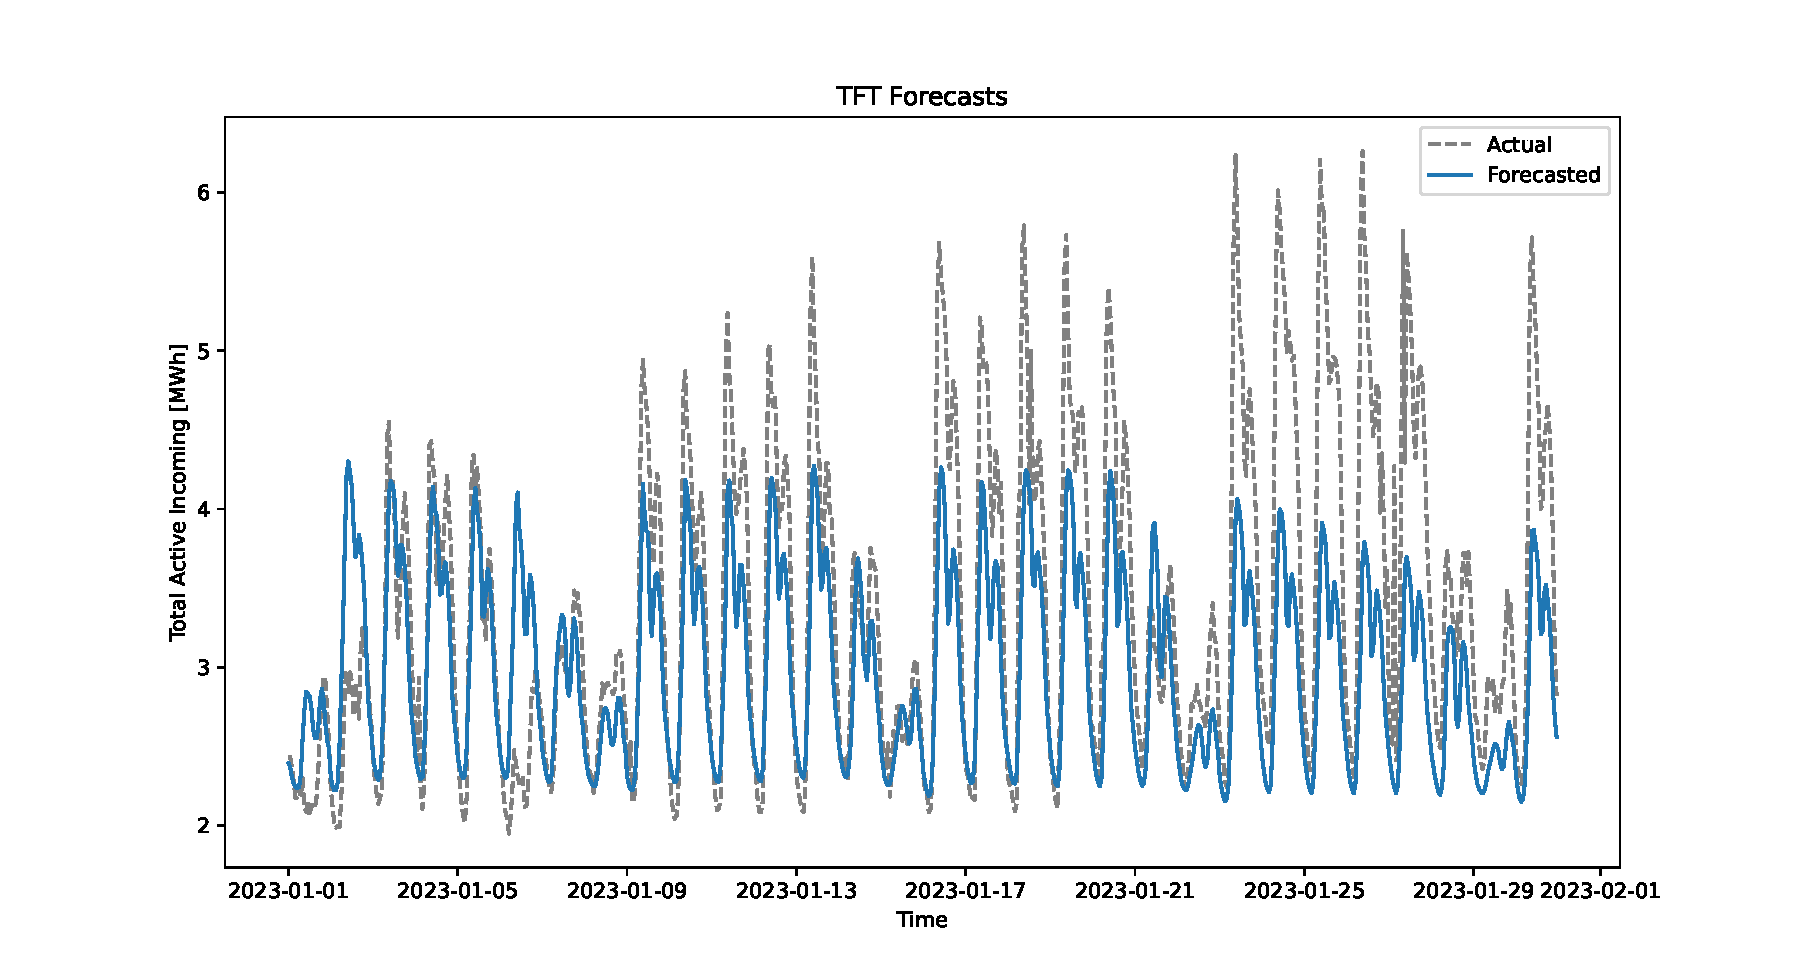
\includegraphics[width=1\textwidth]{images/demand/TFT}
\caption{The forecasts produced by the TFT model for the last split in comparison to the actual values.}
\label{fig:demandtfthourlyforecasts}
\end{figure}

\begin{figure}[H]
\centering
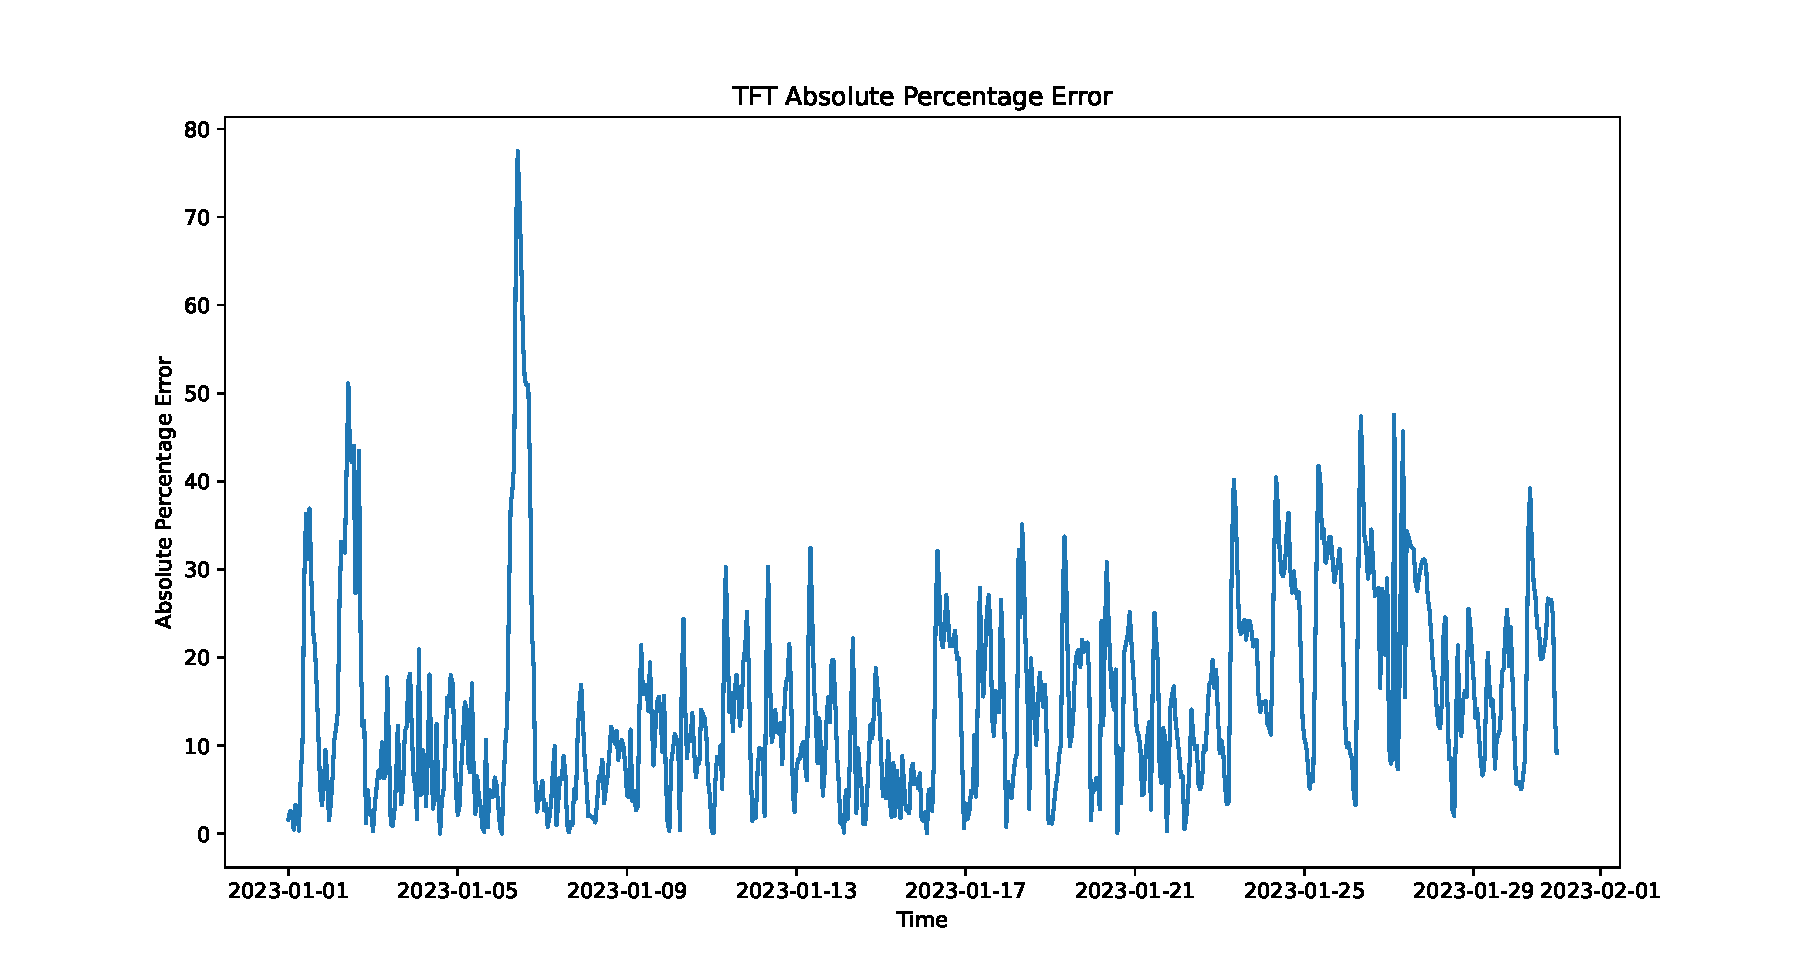
\includegraphics[width=1\textwidth]{images/demand/TFT_mape}
\caption{The absolute percentage error of forecasts produced by the TFT model for the last split in comparison to the actual values.}
\label{fig:demandtfthourlyforecastsmape}
\end{figure}

\begin{figure}[H]
\centering
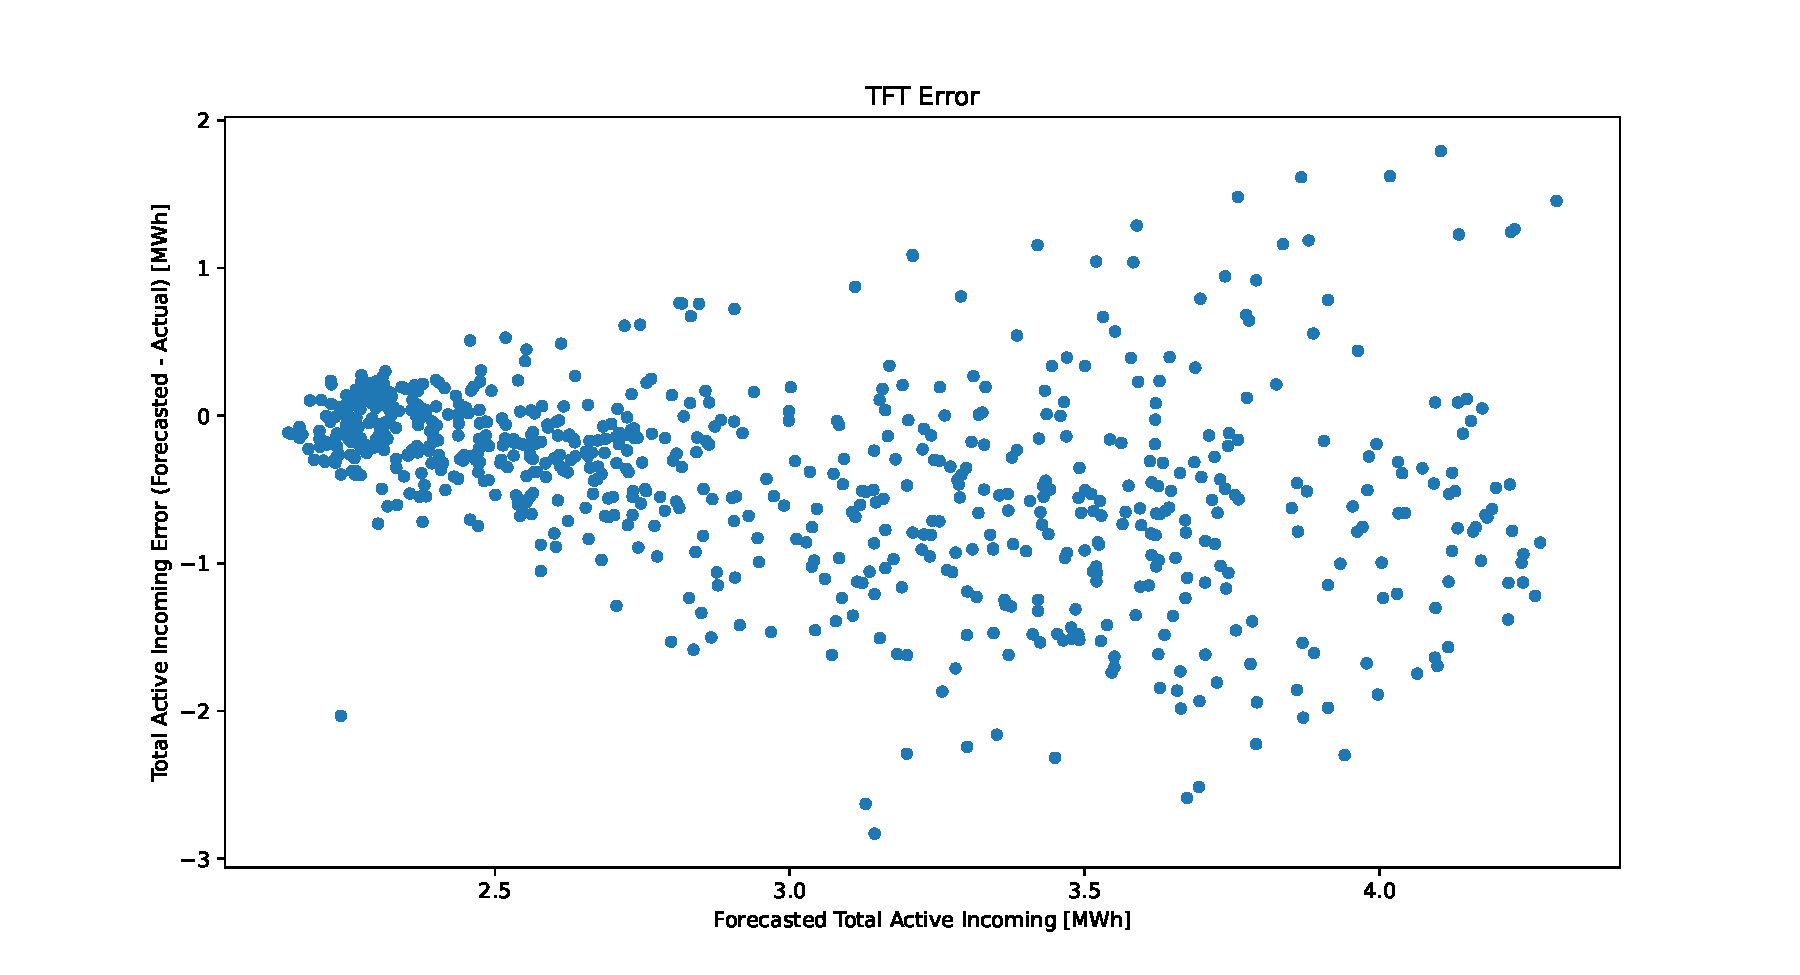
\includegraphics[width=1\textwidth]{images/demand/TFT_error_scatter_plot_predicted}
\caption{The scatter plot representing the error of the forecasts produced by the TFT model for the last split in comparison to the actual values.}
\label{fig:demandtfthourlyforecastsscatterplot}
\end{figure}

For the daily granularity, the models start with 249 entries as training and predict every time 30 entries until reaching the last prediction instant where the model has a training size of 579.
The results for daily granularity are reported in table~\ref{tab:demanddailyresults}.
In this case, TFT is no longer the best-performing model, probably due to the fact of 24 times less quantity of data due to the daily granularity.
Though, it is still a well-performing model on both blocked k-fold cross-validation and last split results.
LSTM and CNN perform better in terms of the last split MAPE but present a high blocked k-fold MAPE, as in the case of the hourly granularity probably that to the increase of data, the results on the last time slots improved in a significant way.
Also, the boosters present very good results on the last time split and also on the blocked k-fold validation showing consistency over time and good results also with few training data. 

\begin{table}[H]
\centering
\begin{tabular}{|c|c|c|}
\hline
\textbf{Model} & \textbf{Blocked k-fold} & \textbf{Test on the last split}\\
 & \textbf{cross-validation MAPE} & \textbf{MAPE}\\
\hline
CNN & 50.55 $\pm$ 36.81 & 7.49\\
\hline
XGBRegressor & 12.96 $\pm$ 4.36 & 7.65\\
\hline
HistGradientBoostingRegressor & 13.02 $\pm$ 5.54 & 9.81\\
\hline
LSTM & 29.60 $\pm$ 13.81 & 14.51\\
\hline
TFT & 13.73 $\pm$ 5.06 & 14.88\\
\hline
One Week Baseline & 11.50 $\pm$ 4.78 & 18.40\\
\hline
SARIMA & 11.92 $\pm$ 7.04 & 19.63\\
\hline
GRU & 28.76 $\pm$ 29.26 & 20.47\\
\hline
One Day Baseline & 22.80 $\pm$ 8.21 & 21.51\\
\hline
Prophet & 19.06 $\pm$ 10.81 & 26.33\\
\hline
SVR & 53.63 $\pm$ 22.39 & 39.82\\
\hline
\end{tabular}
\caption{Table summarizing the results for daily granularity.}
\label{tab:demanddailyresults}
\end{table}

The results for daily granularity at forecasting time on the last time slot including also the combinations of different techniques and the AutoML approach are reported in table~\ref{tab:demanddailyresultsforecast}.
In this case, the impact of the combinations is not so evident and does not improve the results in all the cases.
AutoML presents not very good results being worse than the one-week baseline, this is probably due to the scarcity of training data and the fact of AutoML of trying very complex architectures when also simple ones may work well in certain cases.
It can also be noticed that surprisingly for some of the best-performing models the MAPE on the first week of data is higher than the one on the whole month of data.
This probably can be explained by the fact that the first week of the last split has a less regular pattern due to the Christmas holidays compared to the following ones.

\begin{table}[H]
\centering
\begin{tabular}{|c|c|c|}
\hline
\textbf{Model} & \textbf{Test on the last split} & \textbf{Test on the last split}\\
 & \textbf{one-week MAPE} & \textbf{one-month MAPE}\\
\hline
CNN & 8.36 & 7.49\\
\hline
XGBRegressor & 11.78 & 7.65\\
\hline
HistGradientBoostingRegressor & 12.42 & 9.81\\
\hline
CNN + One Week Baseline & 8.33 & 12.28\\
\hline
LSTM + One Week Baseline & 11.19 & 12.91\\
\hline
LSTM & 18.21 & 14.51\\
\hline
TFT & 12.65 & 14.88\\
\hline
LSTM + One Week Baseline + & 8.81 & 15.91\\
Prophet & & \\
\hline
CNN + One Week Baseline + & 11.34 & 16.96\\
Prophet & & \\
\hline
LSTM + One Day Baseline + & 9.82 & 17.29\\
One Week Baseline + Prophet & & \\
\hline
CNN + One Day Baseline + & 10.88 & 17.88\\
One Week Baseline + Prophet & & \\
\hline
One Week Baseline & 9.63 & 18.40\\
\hline
GRU + One Week Baseline & 9.15 & 19.18\\
\hline
SARIMA & 11.23 & 19.63\\
\hline
GRU & 10.87 & 20.47\\
\hline
AutoML & 10.61 & 20.98\\
\hline
GRU + One Day Baseline + & 11.29 & 21.34\\
One Week Baseline + Prophet & & \\
\hline
One Day Baseline & 13.14 & 21.51\\
\hline
GRU + One Week Baseline + & 11.89 & 21.56\\
Prophet & & \\
\hline
One Day Baseline + & 11.72 & 21.69\\
One Week Baseline + Prophet & & \\
\hline
One Week Baseline + Prophet & 12.83 & 22.21\\
\hline
Prophet & 17.35 & 26.33\\
\hline
SVR & 58.09 & 39.82\\
\hline
\end{tabular}
\caption{Table summarizing the results for hourly granularity at forecasting time.}
\label{tab:demanddailyresultsforecast}
\end{table}

The forecasts produced by the CNN model for the last split in comparison to the actual values are reported in figure~\ref{fig:demandcnndailyforecasts}.
It can be noticed that for the first three weeks, it follows the signal very accurately and the last week is increasing correctly but not enough as the actual values.
The absolute percentage error of forecasts produced by the CNN model for the last split in comparison to the actual values is reported in figure~\ref{fig:demandcnndailyforecastsmape}.
It can be shown that except for some peaks, the percentage error stays below 10\%.
Finally, the scatter plot representing the error of the forecasts produced by the CNN model for the last split in comparison to the actual values is reported in figure~\ref{fig:demandcnndailyforecastsscatterplot}.
This scatter plot demonstrates that there is no bias even though it seems that when predicting high values it is missing some extra quantity in the forecasts, this is probably true in the specific considered last split and in particular the last week.

\begin{figure}[H]
\centering
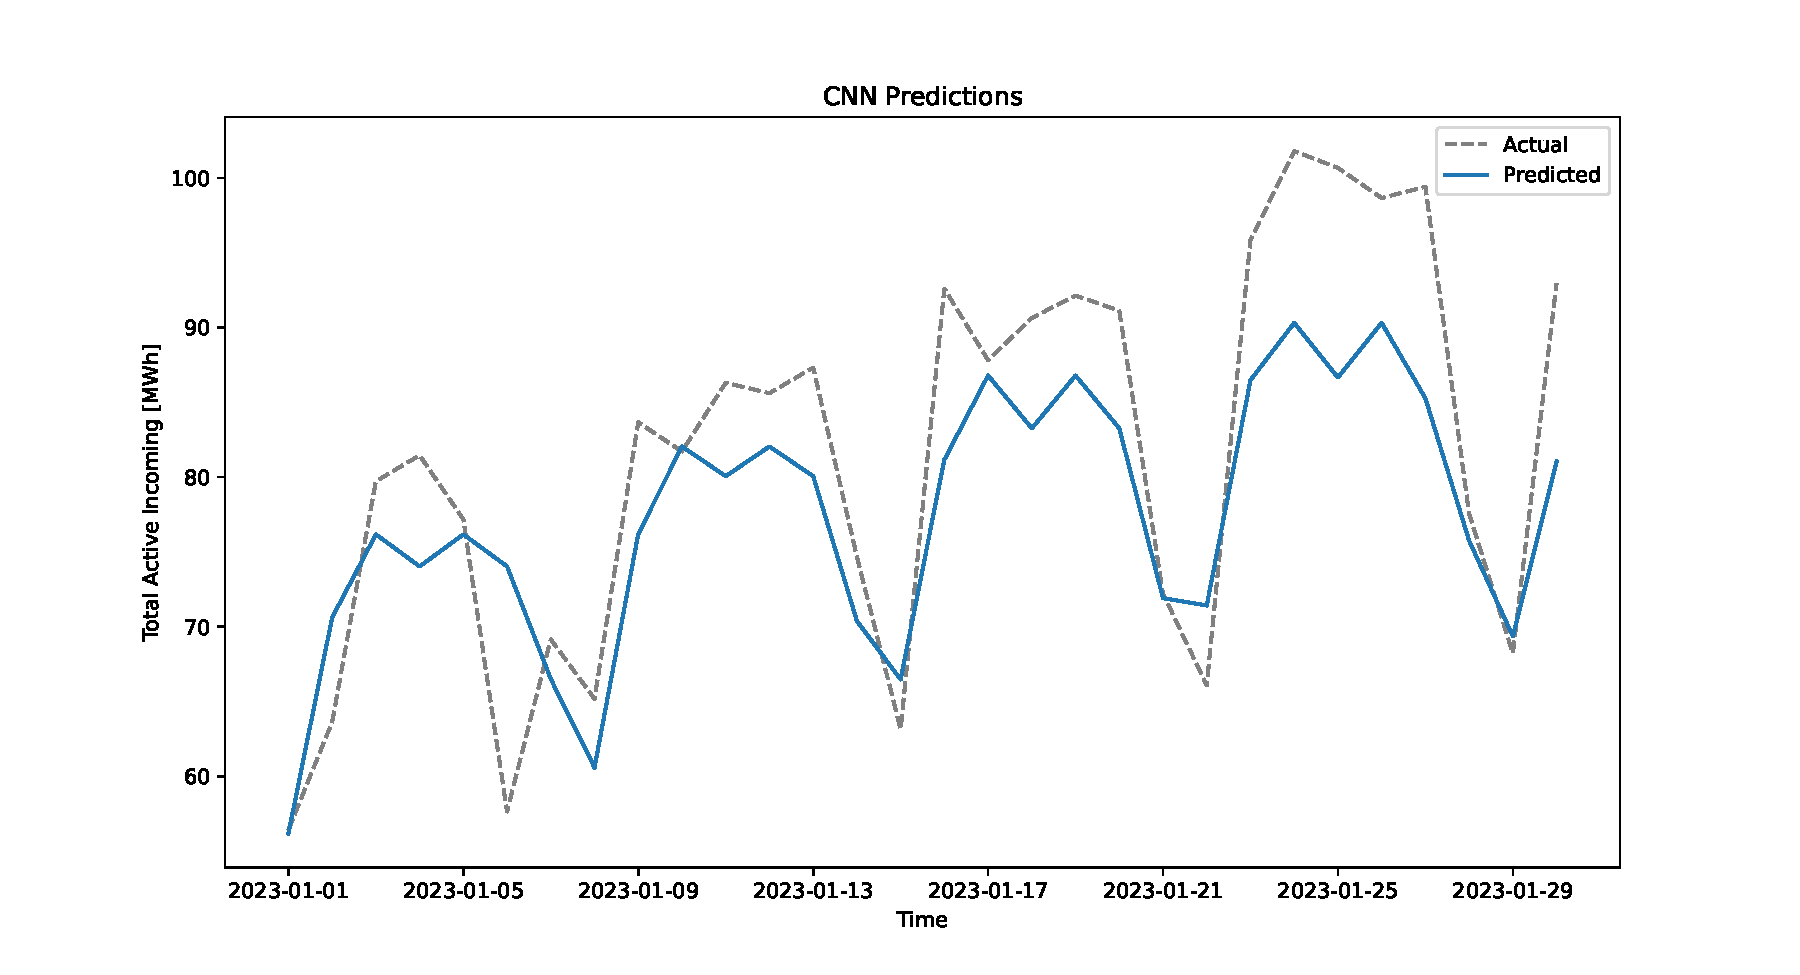
\includegraphics[width=1\textwidth]{images/demand/CNN_daily_aggregated}
\caption{The forecasts produced by the CNN model for the last split in comparison to the actual values.}
\label{fig:demandcnndailyforecasts}
\end{figure}

\begin{figure}[H]
\centering
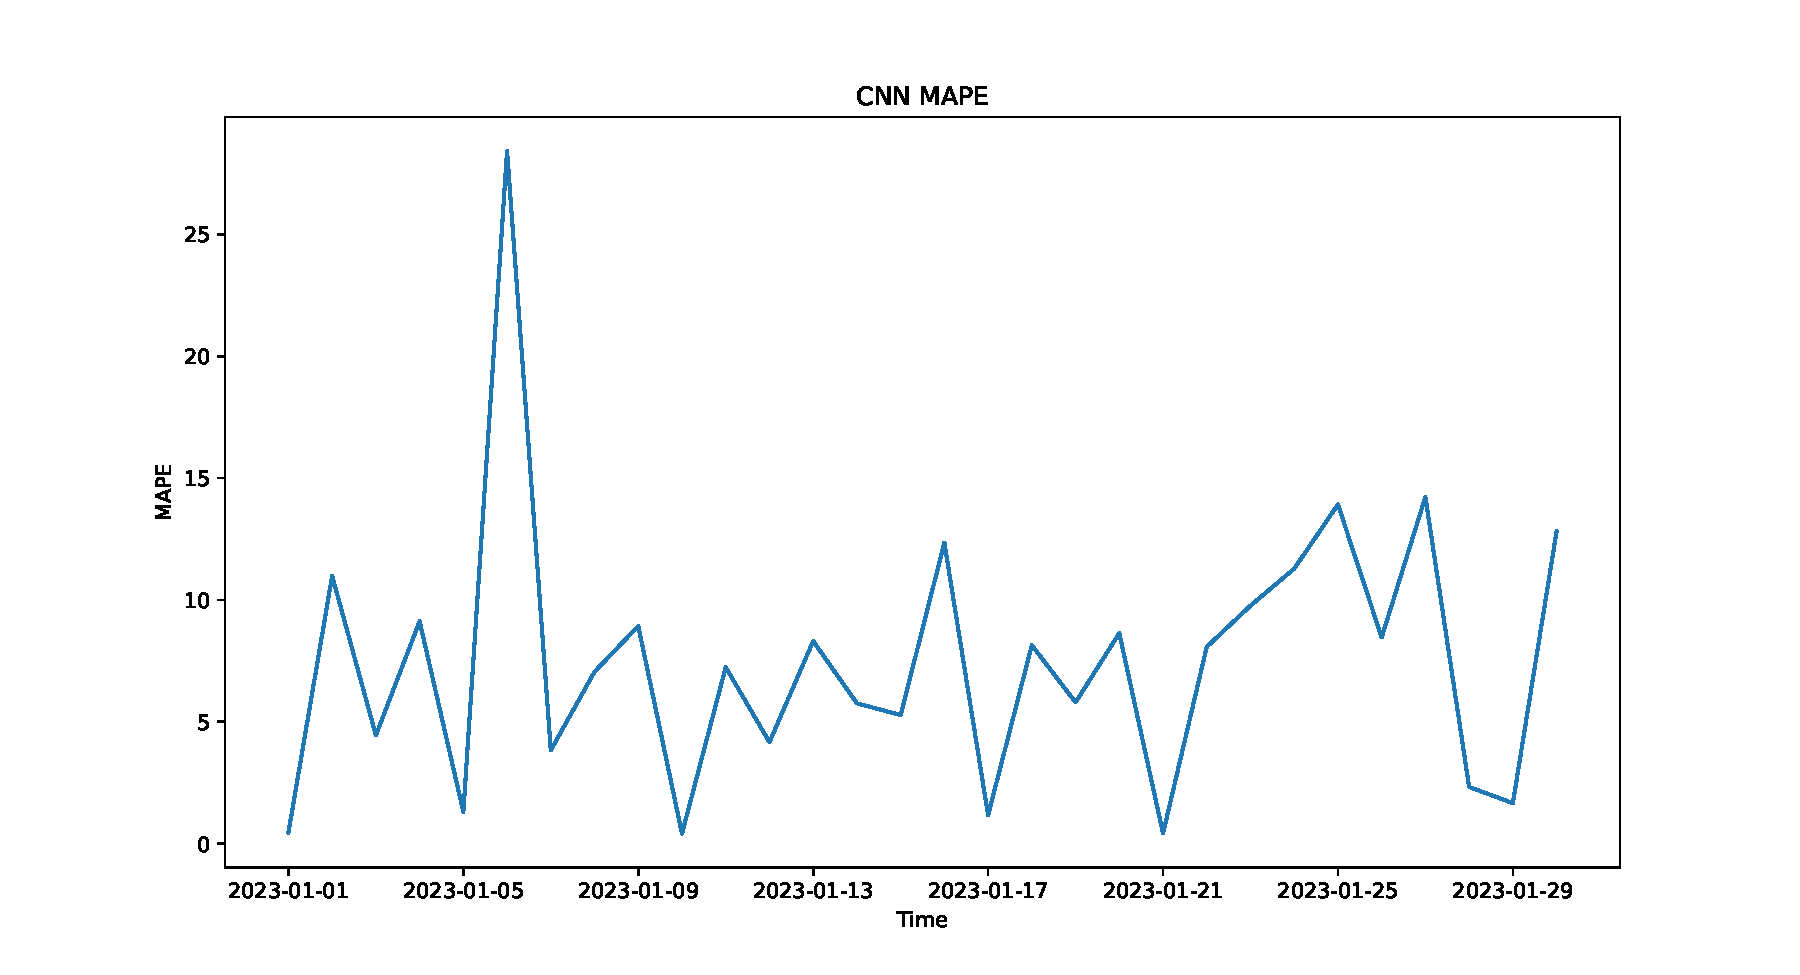
\includegraphics[width=1\textwidth]{images/demand/CNN_daily_aggregated_mape}
\caption{The absolute percentage error of forecasts produced by the CNN model for the last split in comparison to the actual values.}
\label{fig:demandcnndailyforecastsmape}
\end{figure}

\begin{figure}[H]
\centering
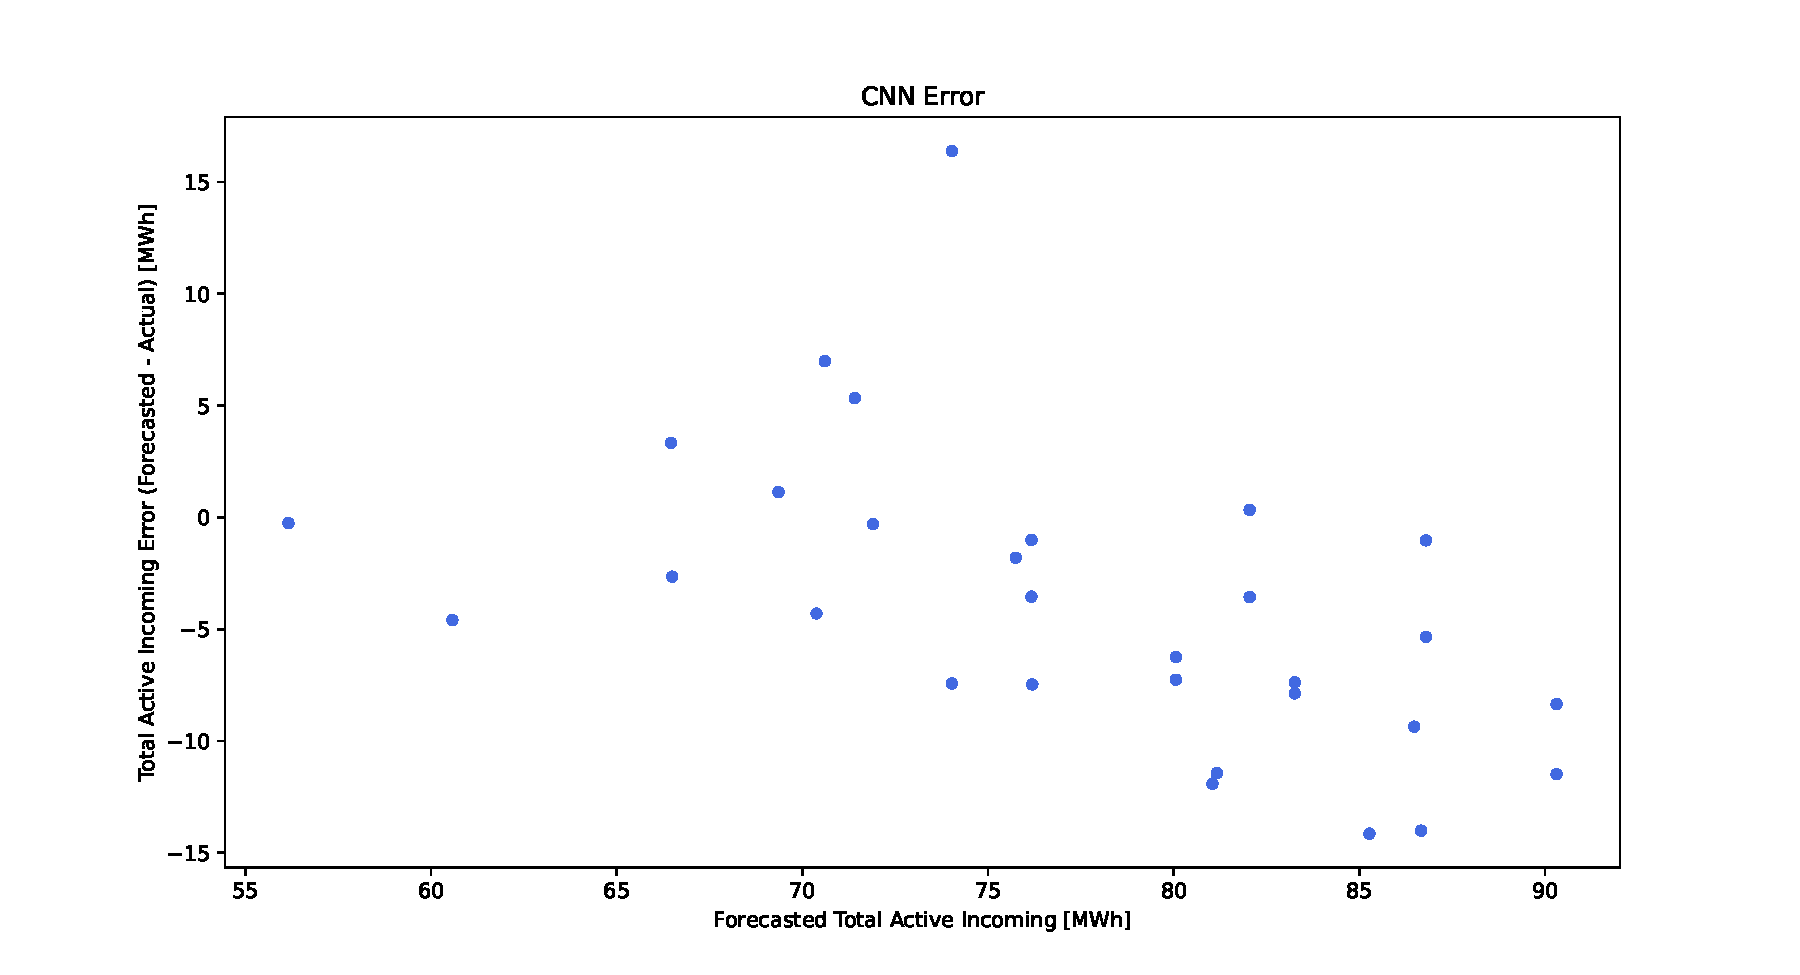
\includegraphics[width=1\textwidth]{images/demand/CNN_error_scatter_plot_predicted_daily_aggregated}
\caption{The scatter plot representing the error of the forecasts produced by the CNN model for the last split in comparison to the actual values.}
\label{fig:demandcnndailyforecastsscatterplot}
\end{figure}


\section{Electricity production forecasting}
\label{sec:productionval}
\vspace{0.2 cm}

As described in the data preprocessing in Chapter~\ref{cha:implementation}, single PV plant production data are aggregated to obtain the aggregated production data over the PV plants.
The target of the predictions is the mean percentage of production, which is calculated as the division of the total produced energy by the total nominal power of the PV plants.
This allows us to have a bounded value from 0 to 100 from which it is possible to obtain the total produced energy simply by multiplying it by the total nominal power of the PV plants.
This was also done since PV plants are added over time and this was unpredictable, this results in predicting the percentage of production of the PV plants.
This data is analyzed to get some descriptive analytics before finding adequate models to forecast the production.

The time series decomposition using an additive model of the hourly percentage of production data considering as period of the time series a day is reported in figure~\ref{fig:productiondecomposition}.
It showed a considerable amount of noise, comparable to seasonality and trend in magnitude.
The trend component exhibits a clear peak during the summer season.
As expected, the seasonality component appears to have the most significant impact on the time series.

\begin{figure}[H]
\centering
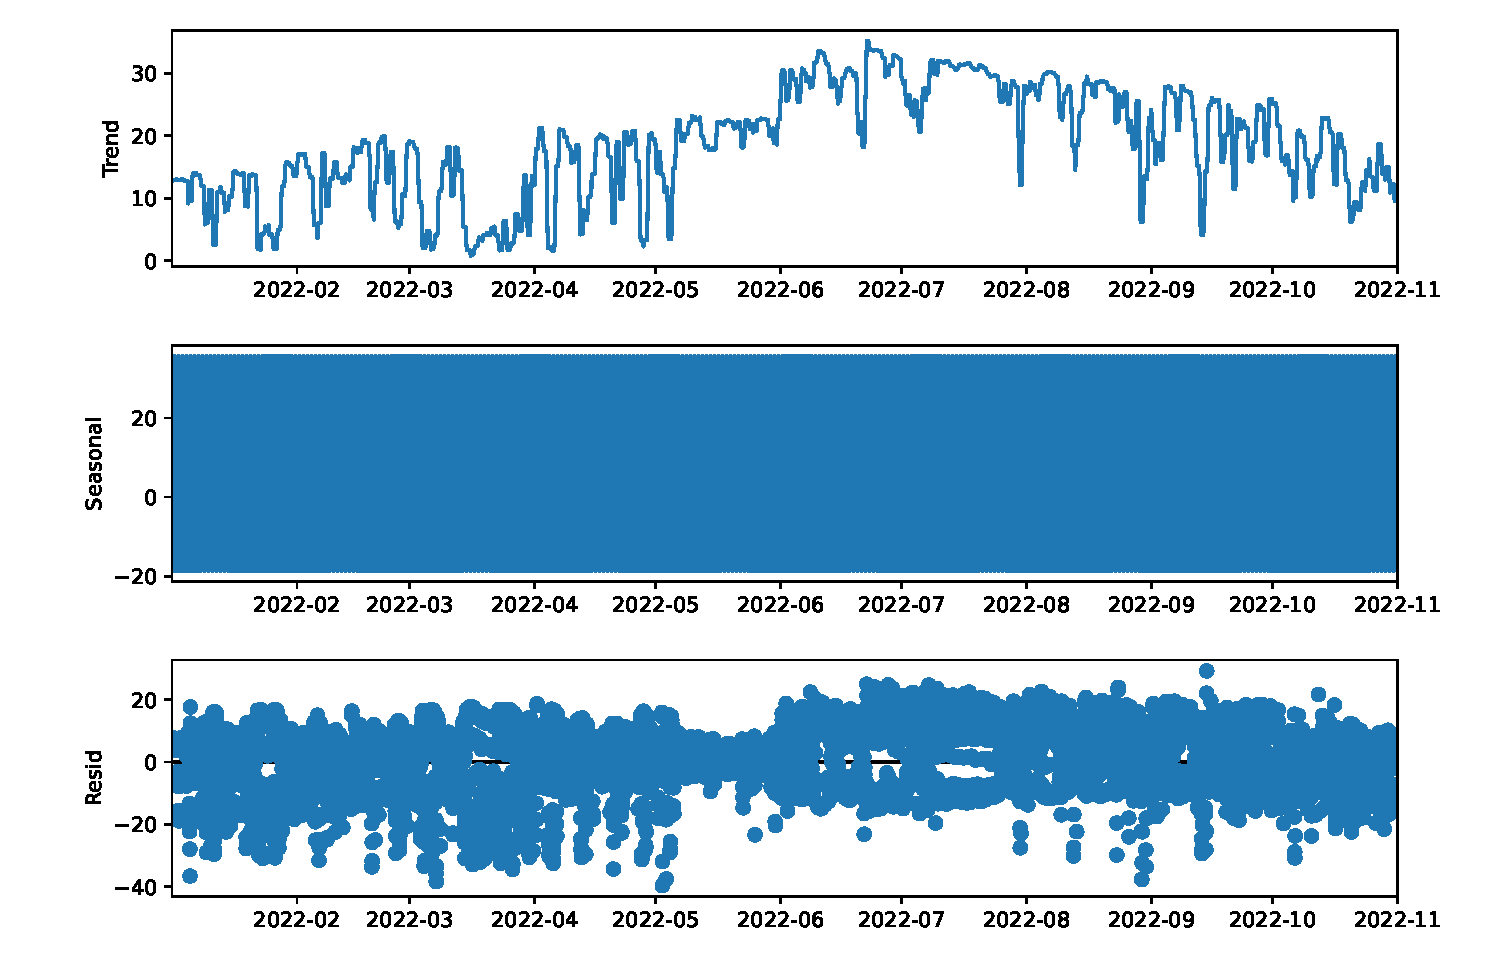
\includegraphics[width=0.475\textwidth]{images/production/hourly_decomposition}
\caption{The time series decomposition of the hourly percentage of production data considering as period of the time series a day.}
\label{fig:productiondecomposition}
\end{figure}

The auto-correlation of the hourly percentage of production data is reported in figure~\ref{fig:productioncorrelation}.
It shows a high auto-correlation value in the closest time lag and also at every 24 hours, with the value slightly decreasing as the lag increases over days.
This indicates that the production data from the closest time lag and those corresponding to the same hour in the preceding days may be valuable features for predicting a time instant's production.
A reasonable balance can be achieved by incorporating the production data from the past 14 days.

\begin{figure}[H]
\centering
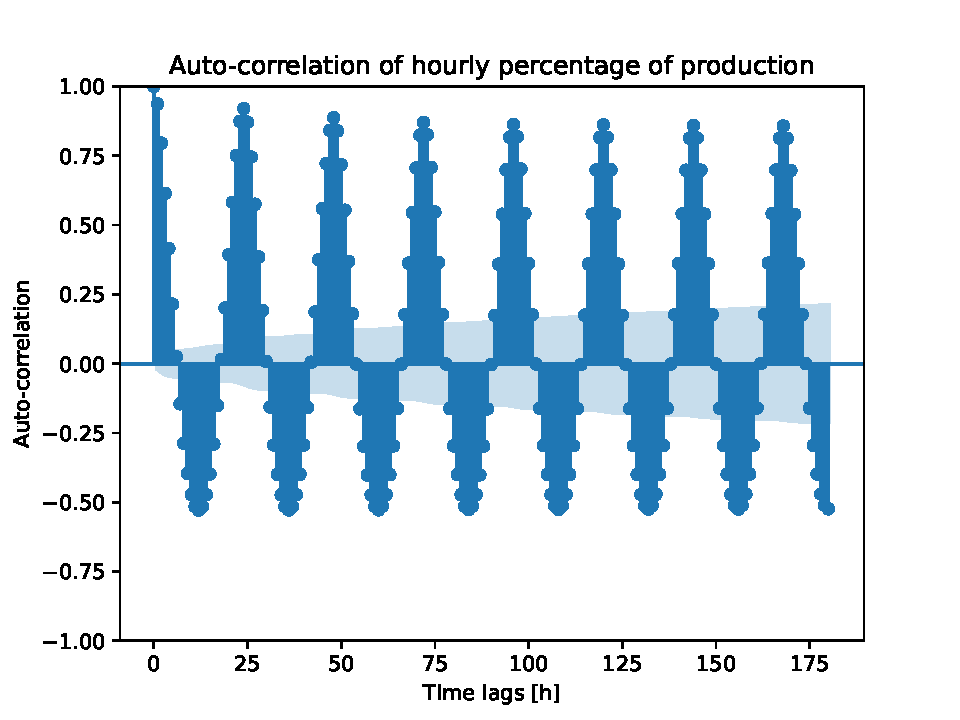
\includegraphics[width=0.4\textwidth]{images/production/hourly_correlation_week_range}
\caption{The auto-correlation of the hourly percentage of production data.}
\label{fig:productioncorrelation}
\end{figure}

The coefficients given by the Fourier transform for the hourly percentage of production data are reported in figure~\ref{fig:productionft}.
The graphical representation clearly shows a main frequency at the daily periodicity.
Other minor peaks are present mostly at multiples of the 1/day frequency.

\begin{figure}[H]
\centering
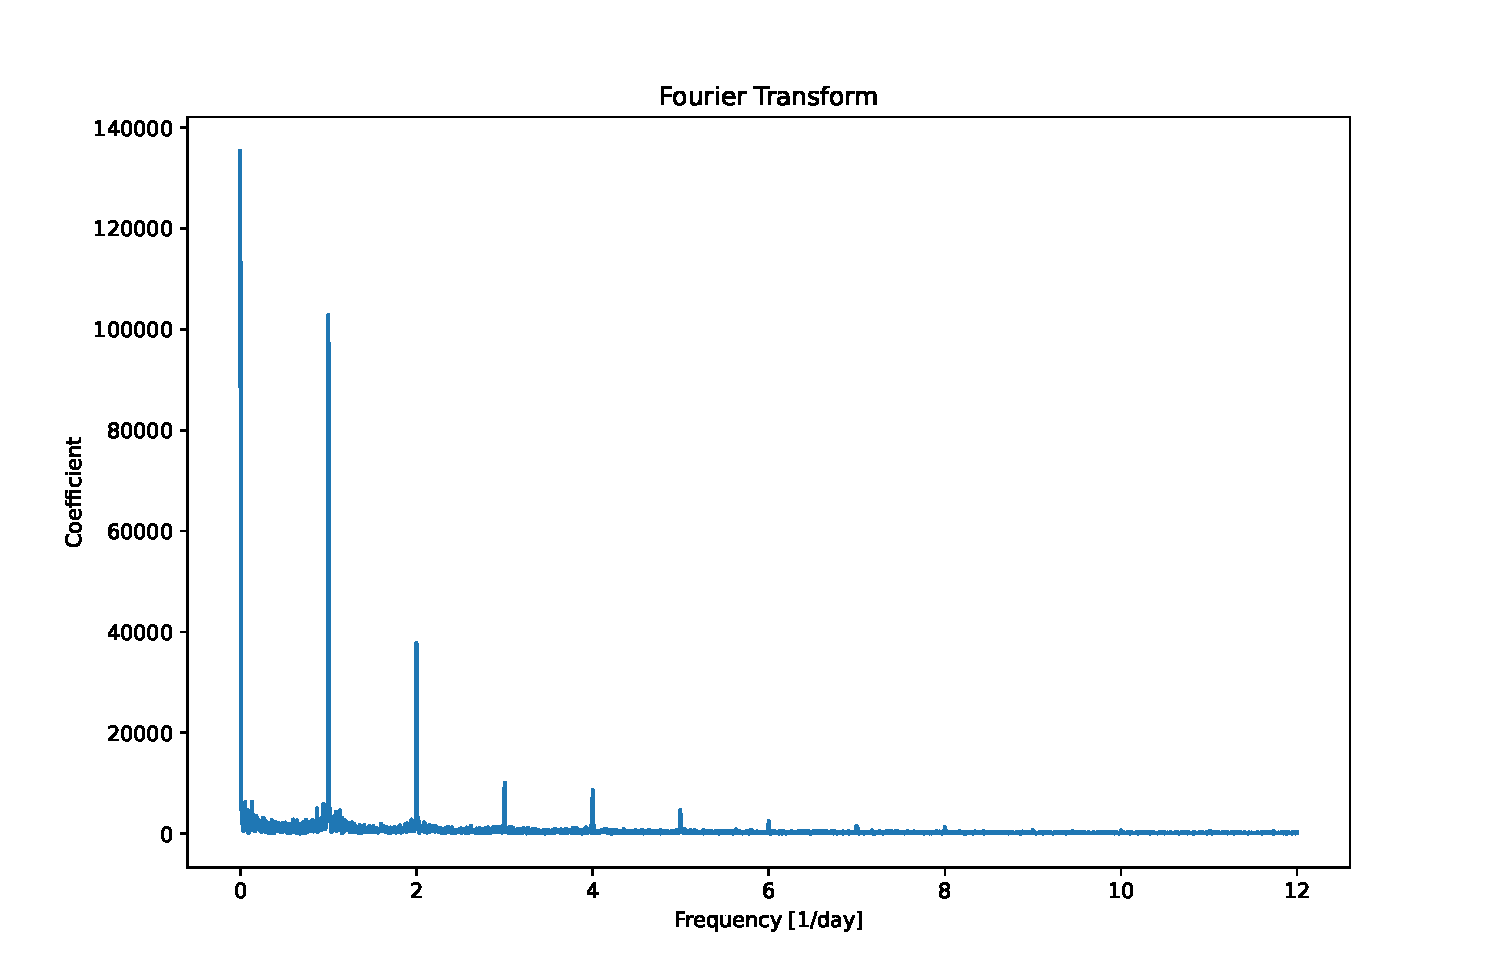
\includegraphics[width=0.4\textwidth]{images/production/ft_hour_day}
\caption{The coefficients given by the Fourier transform for the hourly percentage of production data.}
\label{fig:productionft}
\end{figure}

The daily percentage of production data is reported in figure~\ref{fig:productiondataplotday}.

\begin{figure}[H]
\centering
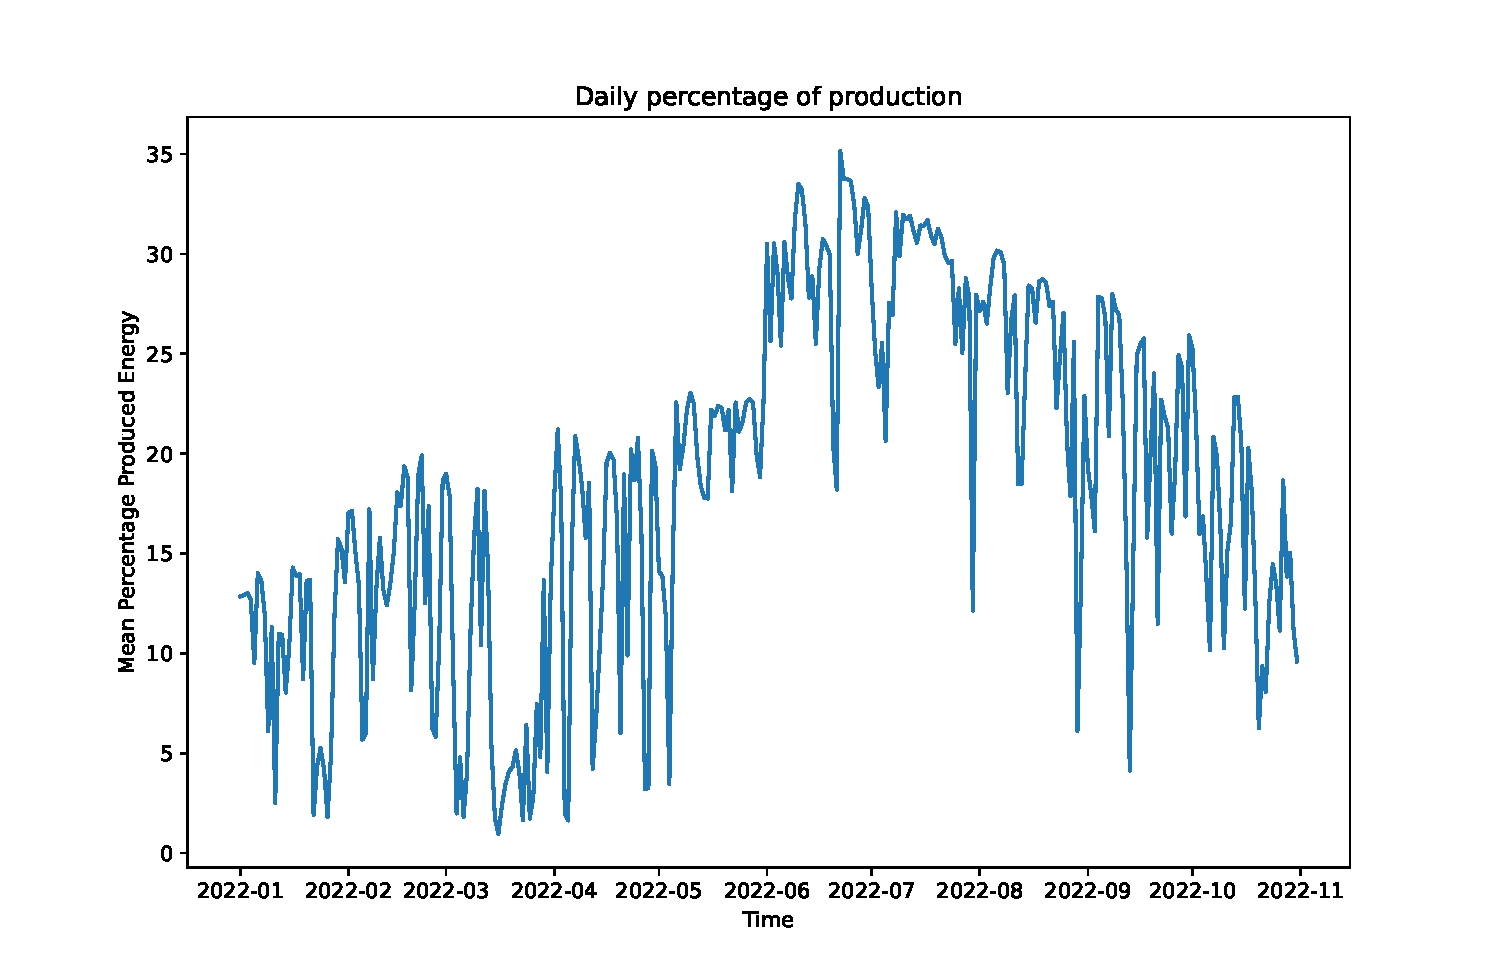
\includegraphics[width=0.5\textwidth]{images/production/data_day_aggregated_plot}
\caption{The daily percentage of production data.}
\label{fig:productiondataplotday}
\end{figure}

The time series decomposition using an additive model of the daily percentage of production data considering as period of the time series a week is reported in figure~\ref{fig:productiondecompositionday}.
It showed a considerable amount of noise, comparable to the trend in magnitude when not in the summer season.
The trend component exhibits a clear peak during the summer season and appears to be the significant component of the time series.
In this case, considering a weekly period, the seasonality component appears to not have a significant impact on the time series.

\begin{figure}[H]
\centering
\includegraphics[width=0.475\textwidth]{images/production/daily_aggregated_decomposition}
\caption{The time series decomposition of the daily percentage of production data considering as period of the time series a week.}
\label{fig:productiondecompositionday}
\end{figure}

The auto-correlation of the daily percentage of production data is reported in figure~\ref{fig:productioncorrelationday}.
It shows a high auto-correlation value in the closest time lag and then a slight decrease as the lag increases over days.

\begin{figure}[H]
\centering
\includegraphics[width=0.4\textwidth]{images/production/daily_aggregated_correlation}
\caption{The auto-correlation of the daily percentage of production data.}
\label{fig:productioncorrelationday}
\end{figure}

\begin{figure}[H]
\centering
\includegraphics[width=0.4\textwidth]{images/production/ft_day}
\caption{The coefficients given by the Fourier transform for the daily percentage of production data.}
\label{fig:productionftday}
\end{figure}

The coefficients given by the Fourier transform for the daily percentage of production data are reported in figure~\ref{fig:productionftday}.
As expected from the time series decomposition, the graphical representation exhibits that there are no main frequencies in the daily percentage of production.

Basic data is enhanced with the air temperature, the apparent temperature, the relative humidity, the wind speed, the wind direction, the pressure altimeter, the visibility, the sky coverage, the diffuse horizontal irradiance, the direct normal irradiance, the global horizontal irradiance, the solar radiation, the UV index, the solar elevation angle, and the solar azimuth angle.
To assess the relationship between these weather variables and the percentage of production, two correlation coefficients were used: Pearson's correlation coefficient and Spearman's rank correlation coefficient.
Pearson's correlation coefficient measures the strength of the linear relationship between two variables, while Spearman's rank correlation coefficient measures the strength of the monotonic relationship.
The pearsonr and spearmanr methods of the SciPy library were used to compute the correlation with weather data.
The results showed that the hourly percentage of production data had:
\begin{itemize}
  \item a Pearson correlation coefficient of $0.5621$ and a Spearman's rank correlation coefficient of $0.5185$ with respect to the air temperature data;
  \item a Pearson correlation coefficient of $0.5410$ and a Spearman's rank correlation coefficient of $0.5032$ with respect to the apparent temperature data;
  \item a Pearson correlation coefficient of $-0.6318$ and a Spearman's rank correlation coefficient of $-0.5969$ with respect to the relative humidity data;
  \item a Pearson correlation coefficient of $0.3105$ and a Spearman's rank correlation coefficient of $0.3237$ with respect to the wind speed data;
  \item a Pearson correlation coefficient of $-0.1919$ and a Spearman's rank correlation coefficient of $-0.2155$ with respect to the wind direction data;
  \item a Pearson correlation coefficient of $-0.2092$ and a Spearman's rank correlation coefficient of $-0.2645$ with respect to the pressure altimeter data;
  \item a Pearson correlation coefficient of $-0.0132$ and a Spearman's rank correlation coefficient of $0.0355$ with respect to the visibility data;
  \item a Pearson correlation coefficient of $-0.2822$ and a Spearman's rank correlation coefficient of $-0.2375$ with respect to the sky coverage data;
  \item a Pearson correlation coefficient of $0.8559$ and a Spearman's rank correlation coefficient of $0.9340$ with respect to the diffuse horizontal irradiance data;
  \item a Pearson correlation coefficient of $0.8399$ and a Spearman's rank correlation coefficient of $0.9315$ with respect to the direct normal irradiance data;
  \item a Pearson correlation coefficient of $0.8791$ and a Spearman's rank correlation coefficient of $0.9357$ with respect to the global horizontal irradiance data;
  \item a Pearson correlation coefficient of $0.9073$ and a Spearman's rank correlation coefficient of $0.9472$ with respect to the solar radiation data;
  \item a Pearson correlation coefficient of $0.8571$ and a Spearman's rank correlation coefficient of $0.9392$ with respect to the UV index data;
  \item a Pearson correlation coefficient of $0.8107$ and a Spearman's rank correlation coefficient of $0.9057$ with respect to the solar elevation angle data;
  \item a Pearson correlation coefficient of $0.0450$ and a Spearman's rank correlation coefficient of $0.0465$ with respect to the solar azimuth angle data.
\end{itemize}
It can be noticed that both the coefficients indicate a moderate to strong correlation between the hourly percentage of production and several weather features, including the air temperature, the apparent temperature, the relative humidity, the diffuse horizontal irradiance, the direct normal irradiance, the global horizontal irradiance, the solar radiation, the UV index, and the solar elevation angle.
Therefore, these features are chosen to be incorporated into the prediction models, while the other weather features show weaker correlations and are not considered.

The results showed that the daily percentage of production data had:
\begin{itemize}
  \item a Pearson correlation coefficient of $0.7632$ and a Spearman's rank correlation coefficient of $0.7721$ with respect to the air temperature data;
  \item a Pearson correlation coefficient of $0.7434$ and a Spearman's rank correlation coefficient of $0.7471$ with respect to the apparent temperature data;
  \item a Pearson correlation coefficient of $-0.7598$ and a Spearman's rank correlation coefficient of $-0.7474$ with respect to the relative humidity data;
  \item a Pearson correlation coefficient of $0.1773$ and a Spearman's rank correlation coefficient of $0.3769$ with respect to the wind speed data;
  \item a Pearson correlation coefficient of $-0.2405$ and a Spearman's rank correlation coefficient of $-0.2689$ with respect to the wind direction data;
  \item a Pearson correlation coefficient of $-0.2506$ and a Spearman's rank correlation coefficient of $-0.2559$ with respect to the pressure altimeter data;
  \item a Pearson correlation coefficient of $0.2545$ and a Spearman's rank correlation coefficient of $0.3259$ with respect to the visibility data;
  \item a Pearson correlation coefficient of $-0.7004$ and a Spearman's rank correlation coefficient of $-0.6542$ with respect to the sky coverage data;
  \item a Pearson correlation coefficient of $0.6244$ and a Spearman's rank correlation coefficient of $0.6939$ with respect to the diffuse horizontal irradiance data;
  \item a Pearson correlation coefficient of $0.6216$ and a Spearman's rank correlation coefficient of $0.6923$ with respect to the direct normal irradiance data;
  \item a Pearson correlation coefficient of $0.6305$ and a Spearman's rank correlation coefficient of $0.6988$ with respect to the global horizontal irradiance data;
  \item a Pearson correlation coefficient of $0.7878$ and a Spearman's rank correlation coefficient of $0.8013$ with respect to the solar radiation data;
  \item a Pearson correlation coefficient of $0.8389$ and a Spearman's rank correlation coefficient of $0.8680$ with respect to the UV index data;
  \item a Pearson correlation coefficient of $0.6502$ and a Spearman's rank correlation coefficient of $0.7079$ with respect to the solar elevation angle data;
  \item a Pearson correlation coefficient of $0.1457$ and a Spearman's rank correlation coefficient of $0.2813$ with respect to the solar azimuth angle data.
\end{itemize}
It can be noticed that both the coefficients decreased meaning that the mean weather data over the day is less correlated to the daily percentage of production, compared to the hourly granularity.
Only the hourly granularity is considered since PV plants are highly correlated with weather data and the aggregation over the day loses part of this correlation.

If we were forecasting the production of each PV plant individually, the weather data at the specific locations of the plants would result in a higher correlation with the production data and likely allow the models to produce more accurate forecasts.
However, since we are aggregating the production from multiple PV plants and looking for the overall percentage of production in the hour, using the weather data from a location located in the middle of the PV plants is also acceptable.
In figure~\ref{fig:pvplantsmap}, the locations of the PV plants and of the weather station are reported.

\begin{figure}[H]
\centering
\includegraphics[width=0.8\textwidth]{images/production/pv_plants_map}
\caption{The map of the city of Murcia with indicated the location of the PV plants with a blue icon and of the revelation station with a light blue icon. The distances between each PV plant and the weather station are reported in light blue boxes near the PV plant locations.}
\label{fig:pvplantsmap}
\end{figure}

After this data analysis, the specific parameters used in the models can be explained more in detail.
The parameters for the different models were tested and verified on training data to result in the best-performing models, this was done by trying different values and configurations.
The baseline approach is built considering the repetition of past days since data presents a high correlation with that time instant and could lead to a reasonable baseline performance to achieve.
A simple ARIMA model considers the single hours without seasonally on the week period like for demand prediction since data does not present a relevant correlation with that time instants.
The support vector regressor model uses a radial basis function kernel with a configuration of the C parameter (regularization parameter of squared l2 penalty) to 1.0 to penalize the complexity of the model, and the epsilon parameter defining the epsilon-tube for no penalty to 0.1 as a trade-off between accuracy and generalization.
The hist gradient boosting regressor model uses as loss the absolute error.
The learning rate was set to 0.1, 100 estimators were used and l2 regularization was not set.
The parameters for tree definition are 31 as the maximum number of leaves, depth is not constrained, 20 as the minimum number of samples per leaf, and 255 as the maximum number of bins.
For the extreme gradient boosting regressor model, tree-based models were used and the construction algorithm is automatically chosen by heuristic to choose the fastest method.
It uses a squared loss since this was the supported metric closer to our evaluation metric.
The learning rate was set to 0.3, 100 estimators were used and l2 regularization was set with a weight of 1.0.
The parameters for tree definition are 6 as the maximum depth, and the maximum number of leaves is not constrained.
The Prophet model was built keeping the default parameters for automatically detecting seasonalities and best fitting the training data.

The LSTM model was designed as a 2-layer model with 32 Bidirectional LSTM units in the first layer which use ReLU activation function and sigmoid as recurrent activation function with both dropout and recurrent dropout of 0.02.
The second layer is composed of 16 Bidirectional LSTM units which use ReLU activation function and sigmoid as recurrent activation function without dropout and recurrent dropout.
The output of the layer goes inside a dense unit to output the final prediction.
The model is trained using MAE as loss and Nadam as optimizer with a learning rate of 0.005.

The GRU model was designed as a 2-layer model with 32 Bidirectional GRU units in the first layer which use ReLU activation function and sigmoid as recurrent activation function with both dropout and recurrent dropout of 0.02.
Subsequently, the second layer is composed of 16 Bidirectional GRU units which use ReLU activation function and sigmoid as recurrent activation function without dropout and recurrent dropout.
The output of the layer goes inside a dense unit to output the final prediction.
The model is trained using MAE as loss and Nadam as optimizer with a learning rate of 0.005.

The CNN model was designed as a 2-layer model with a first layer composed of 24 1D Convolutional units with a kernel size of 5 which uses ReLU activation function.
A 1D max polling operation is applied before entering the second layer composed of 16 1D Convolutional units with a kernel size of 3 which use ReLU activation function.
A 1D max polling operation is applied before the flattening operation and entering the final dense unit to output the final prediction.
The model is trained using MAE as loss and Nadam as optimizer with a learning rate of 0.005.

The TFT model was configured with 2 LSTM layers with 16 as hidden size, 4 as attention size, and 8 as hidden continuous size.
The dropout is set to 0.02.
The model is trained using MAE as loss and Nadam as optimizer with a learning rate of 0.005.

12 splits were used for block validation with a test size of a week each time, namely 7 days of data.
The models start with 5280 entries as training and predict every time 168 entries until reaching the last prediction instant where the model has a training size of 7128.
The results for hourly granularity are reported in table~\ref{tab:productionhourlyresults}.
Entries are sorted by best MAE normalized on PV plants' nominal power using the last split as the test set.
The blocked k-fold cross-validation suggests that the hist gradient boosting regressor model has the best MAE, but looking at the last split this is not confirmed.
In fact, the GRU model performs better on the last split, as the other DL models, this seems to confirm what is seen in demand prediction that with the increase of training data, these models perform better.
It can also be noted that all the models are better than the one-day baseline.
Prophet presents not very good results compared to the other models and is close to the baseline as results on the last split while considering the blocked k-fold cross-validation is the only model that performs worse than it,
In this case, the TFT approach does not seem to perform in an optimal way, and its results are close to the ones of LSTM and ARIMA models.

\begin{table}[H]
\centering
\begin{tabular}{|c|c|c|}
\hline
 & \textbf{Blocked k-fold cross-validation} & \textbf{Test on the last split}\\
\textbf{Model} & \textbf{MAE normalized on PV} & \textbf{MAE normalized on PV}\\
 & \textbf{plants' nominal power} & \textbf{plants' nominal power}\\
\hline
GRU & 5.70 $\pm$ 1.78 & 2.79\\
\hline
HistGradientBoostingRegressor & 4.16 $\pm$ 0.99 & 2.98\\
\hline
SVR & 5.20 $\pm$ 1.12 & 3.12\\
\hline
CNN & 5.98 $\pm$ 1.52 & 3.27\\
\hline
XGBRegressor & 4.57 $\pm$ 0.97 & 3.42\\
\hline
LSTM & 5.23 $\pm$ 1.46 & 3.51\\
\hline
TFT & 4.70 $\pm$ 1.39 & 3.60\\
\hline
ARIMA & 5.09 $\pm$ 1.35 & 3.64\\
\hline
Prophet & 7.90 $\pm$ 1.62 & 4.38\\
\hline
One Day Baseline & 6.81 $\pm$ 3.14 & 4.58\\
\hline
\end{tabular}
\caption{Table summarizing the results for hourly granularity.}
\label{tab:productionhourlyresults}
\end{table}

The results for hourly granularity at forecasting time on the last time slot including also the combinations of different techniques and the AutoML approach are reported in table~\ref{tab:productionhourlyresultsforecast}.
The combination of the previous techniques was performed by combining one-day baseline and Prophet with possibly one of LSTM, GRU, or CNN with the intent of trying to improve the robustness of DL models with some stable baselines and Prophet model which internally automatically deals with seasonalities, even though for this task it is not performing very well.
The AutoML approach uses the mean MAPE forecasting as loss and it is launched for 10 hours with a maximum function evaluation time of 2 hours.
Also, the mean MAE forecasting was used but provided worse results.
Then the best ensemble of the found models is returned and can be used to forecast.

\begin{table}[H]
\centering
\begin{tabular}{|c|c|c|}
\hline
 & \textbf{Test on the last split}\\
\textbf{Model} & \textbf{MAE normalized on PV}\\
 & \textbf{plants' nominal power}\\
\hline
GRU & 2.79\\
\hline
HistGradientBoostingRegressor & 2.86\\
\hline
SVR & 3.12\\
\hline
CNN & 3.27\\
\hline
XGBRegressor & 3.35\\
\hline
LSTM + One Day Baseline & 3.37\\
\hline
GRU + One Day Baseline & 3.45\\
\hline
CNN + One Day Baseline & 3.48\\
\hline
LSTM & 3.51\\
\hline
TFT & 3.60\\
\hline
LSTM + One Day Baseline + Prophet & 3.60\\
\hline
ARIMA & 3.64\\
\hline
CNN + One Day Baseline + Prophet & 3.67\\
\hline
GRU + One Day Baseline + Prophet & 3.70\\
\hline
One Day Baseline + Prophet & 4.38\\
\hline
Prophet & 4.38\\
\hline
One Day Baseline & 4.58\\
\hline
AutoML & 5.89\\
\hline
\end{tabular}
\caption{Table summarizing the results for hourly granularity at forecasting time.}
\label{tab:productionhourlyresultsforecast}
\end{table}

\begin{figure}[H]
\centering
\includegraphics[width=1\textwidth]{images/production/GRU_percentage}
\caption{The forecasts produced by the GRU model for the last split in comparison to the actual values.}
\label{fig:productiongruhourlyforecasts}
\end{figure}

\begin{figure}[H]
\centering
\includegraphics[width=1\textwidth]{images/production/GRU_percentage_mae}
\caption{The absolute error of forecasts produced by the GRU model for the last split in comparison to the actual values.}
\label{fig:productiongruhourlyforecastsmae}
\end{figure}

\begin{figure}[H]
\centering
\includegraphics[width=1\textwidth]{images/production/GRU_percentage_error_scatter_plot_predicted}
\caption{The scatter plot representing the error of the forecasts produced by the GRU model for the last split in comparison to the actual values.}
\label{fig:productiongruhourlyforecastsscatterplot}
\end{figure}

Including also combinations and AutoML, there are a few observations that can be done.
The combinations of DL models and the one-week baseline are the most beneficial, but just in the case of LSTM there is an improvement and it is very marginal.
Probably in this case since the baseline and prophet are not well-performing models they are not bringing any significant improvement or robustness to the DL models.
Nonetheless, it might still make sense to investigate the concept of ensemble learning further and optimize this combination at training time to possibly have more robust results at forecasting time.
In this case, AutoML is not able to achieve very good results compared to many other models.
It still has great potential as demonstrated in demand prediction and potentially providing more total training time it can be able to reach better performance.

The forecasts produced by the GRU model for the last split in comparison to the actual values are reported in figure~\ref{fig:productiongruhourlyforecasts}.
It can be noticed that it follows very accurately the signal for most of the test days, for 2 days it underestimates and for one overestimates the actual data.
The absolute error of forecasts produced by the GRU model for the last split in comparison to the actual values is reported in figure~\ref{fig:productiongruhourlyforecastsmae}.
It can be shown that, except for the peak when it overestimates the actual data and some other minor peaks, the error stays below 10\%.
Finally, the scatter plot representing the error of the forecasts produced by the GRU model for the last split in comparison to the actual values is reported in figure~\ref{fig:productiongruhourlyforecastsscatterplot}.
This scatter plot demonstrates that there is no bias and can be also noticed that when the predicted values are low also the error is limited, while when the prediction is high there are both high positive and negative errors.


\section{Consumption baseline forecasting} 
\label{sec:baselineval}
\vspace{0.2 cm}

The consumption data of the three customers are analyzed to get some descriptive analytics before finding adequate models to forecast the consumption baseline of each customer.

\begin{figure}[H]
\begin{minipage}[b]{8.5cm}
\centering
\includegraphics[width=0.95\textwidth]{images/baseline/hourly_decomposition_week_period_customer1}
\subcaption{First customer.}
\label{fig:decompositioncustomer1}
\end{minipage}
\ \hspace{2mm} \
\begin{minipage}[b]{8.5cm}
\centering
\includegraphics[width=0.95\textwidth]{images/baseline/hourly_decomposition_week_period_customer2}
\subcaption{Second customer.}
\label{fig:decompositioncustomer2}
\end{minipage}
\begin{minipage}[b]{17cm}
\centering
\includegraphics[width=0.475\textwidth]{images/baseline/hourly_decomposition_week_period_customer3}
\subcaption{Third customer.}
\label{fig:decompositioncustomer3}
\end{minipage}
\caption{The time series decompositions of the hourly consumption data of the three customers considering as period of the time series a week.}
\end{figure}

The time series decompositions using an additive model of the hourly consumption data of the three customers considering as period of the time series a week are reported in figure~\ref{fig:decompositioncustomer1}, figure~\ref{fig:decompositioncustomer2}, and figure~\ref{fig:decompositioncustomer3}.
All three decompositions show a considerable amount of noise, which is dominant in magnitude compared to the trend and seasonality.
For all the customers the seasonal component appears to not have a significant impact on the time series, with the exception of the second customer for which it is twice high in magnitude with respect to the others.
The trend component has a slight impact, for the first customer it is possible to see a peak in the winter, for the second customer it is present a peak in April, and for the third customer there is not a clear trend.

\begin{figure}[H]
\begin{minipage}[b]{8.5cm}
\centering
\includegraphics[width=0.8\textwidth]{images/baseline/hourly_correlation_week_range_customer1}
\subcaption{First customer.}
\label{fig:correlationcustomer1}
\end{minipage}
\ \hspace{2mm} \
\begin{minipage}[b]{8.5cm}
\centering
\includegraphics[width=0.8\textwidth]{images/baseline/hourly_correlation_week_range_customer2}
\subcaption{Second customer.}
\label{fig:correlationcustomer2}
\end{minipage}
\begin{minipage}[b]{17cm}
\centering
\includegraphics[width=0.4\textwidth]{images/baseline/hourly_correlation_week_range_customer3}
\subcaption{Third customer.}
\label{fig:correlationcustomer3}
\end{minipage}
\caption{The auto-correlations of the hourly consumption data of the three customers.}
\end{figure}

\begin{figure}[H]
\begin{minipage}[b]{8.5cm}
\centering
\includegraphics[width=0.8\textwidth]{images/baseline/ft_hour_week_customer1}
\subcaption{First customer.}
\label{fig:ftcustomer1}
\end{minipage}
\ \hspace{2mm} \
\begin{minipage}[b]{8.5cm}
\centering
\includegraphics[width=0.8\textwidth]{images/baseline/ft_hour_week_customer2}
\subcaption{Second customer.}
\label{fig:ftcustomer2}
\end{minipage}
\begin{minipage}[b]{17cm}
\centering
\includegraphics[width=0.4\textwidth]{images/baseline/ft_hour_week_customer3}
\subcaption{Third customer.}
\label{fig:ftcustomer3}
\end{minipage}
\caption{The coefficients given by the Fourier transform of the hourly consumption data of the three customers.}
\end{figure}

The auto-correlations of the hourly consumption data of the three customers are reported in figure~\ref{fig:correlationcustomer1}, figure~\ref{fig:correlationcustomer2}, and figure~\ref{fig:correlationcustomer3}.
All the customers' consumptions are not very auto-correlated, it can be shown that the maximum auto-correlation value is around 0.5 in the closest time lag and that there is a peak every 24 hours, with a slightly greater value at one week distance.
This indicates that the consumption data from the closest time lag, as well as those corresponding to the same hour in the preceding days and even better in the preceding weeks, may be valuable features for predicting a time instant's demand.
A reasonable balance can be achieved by incorporating the consumption data from the past 14 days.

The coefficients given by the Fourier transform for the hourly consumption data of the three customers are reported in figure~\ref{fig:ftcustomer1}, figure~\ref{fig:ftcustomer2}, and figure~\ref{fig:ftcustomer3}.
The graphical representations show for all the customers a main frequency at the daily periodicity.
Other minor peaks are present mostly at multiples of the 1/day frequency, in particular for the third customer where the 2/day frequency is almost equal to the 1/day.

The daily consumption data of the three customers are reported in figure~\ref{fig:dataplotdaycustomer1}, figure~\ref{fig:dataplotdaycustomer2}, and figure~\ref{fig:dataplotdaycustomer3}.

\begin{figure}[H]
\begin{minipage}[b]{8.5cm}
\centering
\includegraphics[width=1\textwidth]{images/baseline/data_day_aggregated_plot_customer1}
\subcaption{First customer.}
\label{fig:dataplotdaycustomer1}
\end{minipage}
\ \hspace{2mm} \
\begin{minipage}[b]{8.5cm}
\centering
\includegraphics[width=1\textwidth]{images/baseline/data_day_aggregated_plot_customer2}
\subcaption{Second customer.}
\label{fig:dataplotdaycustomer2}
\end{minipage}
\begin{minipage}[b]{17cm}
\centering
\includegraphics[width=0.5\textwidth]{images/baseline/data_day_aggregated_plot_customer3}
\subcaption{Third customer.}
\label{fig:dataplotdaycustomer3}
\end{minipage}
\caption{The daily consumption data of the three customers.}
\end{figure}

The time series decompositions using an additive model of the daily consumption data of the three customers considering as period of the time series a week are reported in figure~\ref{fig:decompositiondaycustomer1}, figure~\ref{fig:decompositiondaycustomer2}, and figure~\ref{fig:decompositiondaycustomer3}.
The decomposition is consistent with the hourly aggregated consumption over the customers.

The auto-correlations of the daily consumption data of the three customers are reported in figure~\ref{fig:correlationdaycustomer1},  figure~\ref{fig:correlationdaycustomer2}, and  figure~\ref{fig:correlationdaycustomer3}.
With the daily granularity, all the customers' consumptions show a slightly high value with respect to the hourly granularity.
It can be shown that for the first and third customers, the auto-correlation value is slightly high in the closest time lag and then decreases with the days, with a slightly greater value at one week distance.
Instead, for the second customer the only relevant values are only at a multiple of 7 days.

The coefficients given by the Fourier transform for the daily consumption data of the three customers are reported in figure~\ref{fig:ftdaycustomer1}, figure~\ref{fig:ftdaycustomer2}, and figure~\ref{fig:ftdaycustomer3}.
The graphical representation exhibits that there are no main frequencies in the daily consumption of the first and third customers.
Instead, for the second customer there is a small peak at the daily periodicity.

As can be noticed from the data, there is high variability in consumption and low auto-correlation, this suggests how it is difficult to produce highly accurate results on a single customer level.
With just the time series of a few users, it is very difficult to learn a well-performing model, having more users it could be possible to learn certain generic trends or standard behaviors.

Basic data is enhanced with the air temperature, the apparent temperature, and the relative humidity since they are considered the only weather features capable of influencing customers' electricity consumption.
To assess the relationship between these weather variables and the consumption of the three customers, two correlation coefficients were used: Pearson's correlation coefficient and Spearman's rank correlation coefficient.
Pearson's correlation coefficient measures the strength of the linear relationship between two variables, while Spearman's rank correlation coefficient measures the strength of the monotonic relationship.
The pearsonr and spearmanr methods of the SciPy library were used to compute the correlation with weather data.

\begin{figure}[H]
\begin{minipage}[b]{8.5cm}
\centering
\includegraphics[width=0.95\textwidth]{images/baseline/daily_aggregated_decomposition_customer1}
\subcaption{First customer.}
\label{fig:decompositiondaycustomer1}
\end{minipage}
\ \hspace{2mm} \
\begin{minipage}[b]{8.5cm}
\centering
\includegraphics[width=0.95\textwidth]{images/baseline/daily_aggregated_decomposition_customer2}
\subcaption{Second customer.}
\label{fig:decompositiondaycustomer2}
\end{minipage}
\begin{minipage}[b]{17cm}
\centering
\includegraphics[width=0.475\textwidth]{images/baseline/daily_aggregated_decomposition_customer3}
\subcaption{Third customer.}
\label{fig:decompositiondaycustomer3}
\end{minipage}
\label{fig:decompositiondaycustomer}
\caption{The time series decompositions of the daily consumption data of the three customers considering as period of the time series a week.}
\end{figure}

\begin{figure}[H]
\begin{minipage}[b]{8.5cm}
\centering
\includegraphics[width=0.8\textwidth]{images/baseline/daily_aggregated_correlation_customer1}
\subcaption{First customer.}
\label{fig:correlationdaycustomer1}
\end{minipage}
\ \hspace{2mm} \
\begin{minipage}[b]{8.5cm}
\centering
\includegraphics[width=0.8\textwidth]{images/baseline/daily_aggregated_correlation_customer2}
\subcaption{Second customer.}
\label{fig:correlationdaycustomer2}
\end{minipage}
\begin{minipage}[b]{17cm}
\centering
\includegraphics[width=0.4\textwidth]{images/baseline/daily_aggregated_correlation_customer3}
\subcaption{Third customer.}
\label{fig:correlationdaycustomer3}
\end{minipage}
\caption{The auto-correlations of the daily consumption data of the three customers.}
\end{figure}

\begin{figure}[H]
\begin{minipage}[b]{8.5cm}
\centering
\includegraphics[width=0.8\textwidth]{images/baseline/ft_day_customer1}
\subcaption{First customer.}
\label{fig:ftdaycustomer1}
\end{minipage}
\ \hspace{2mm} \
\begin{minipage}[b]{8.5cm}
\centering
\includegraphics[width=0.8\textwidth]{images/baseline/ft_day_customer2}
\subcaption{Second customer.}
\label{fig:ftdaycustomer2}
\end{minipage}
\begin{minipage}[b]{17cm}
\centering
\includegraphics[width=0.4\textwidth]{images/baseline/ft_day_customer3}
\subcaption{Third customer.}
\label{fig:ftdaycustomer3}
\end{minipage}
\caption{The coefficients given by the Fourier transform of the daily consumption data of the three customers.}
\end{figure}

The results showed that the hourly consumption data of the three customers had:
\begin{itemize}
  \item a Pearson correlation coefficient of $-0.2491$, $0.0240$, and $-0.1338$ respectively and a Spearman's rank correlation coefficient of $-0.2088$, $0.1304$, and $-0.0196$ respectively with respect to the air temperature data;
  \item a Pearson correlation coefficient of $-0.2434$, $0.0266$, and $-0.1356$ respectively and a Spearman's rank correlation coefficient of $-0.2082$, $0.1305$, and $-0.0207$ respectively with respect to the apparent temperature data;
  \item a Pearson correlation coefficient of $0.1193$, $-0.0845$, and $-0.0985$ respectively and a Spearman's rank correlation coefficient of $0.1491$, $-0.1048$, and $-0.1123$ respectively with respect to the relative humidity data.
\end{itemize}
It can be noticed that both the coefficients indicate a weak correlation between the weather variables and the consumption of the three customers, nevertheless, it may still be useful to incorporate weather data into the prediction models since also the auto-correlation values are not particularly high.

The results showed that the daily consumption data of the three customers had:
\begin{itemize}
  \item a Pearson correlation coefficient of $-0.5542$, $-0.2341$, and $-0.6727$ respectively and a Spearman's rank correlation coefficient of $-0.5164$, $-0.2592$, and $-0.6978$ respectively with respect to the air temperature data;
  \item a Pearson correlation coefficient of $-0.5361$, $-0.2329$, and $-0.6787$ respectively and a Spearman's rank correlation coefficient of $-0.5166$, $-0.2584$, and $-0.7004$ respectively with respect to the apparent temperature data;
  \item a Pearson correlation coefficient of $0.1264$, $0.0199$, and $0.1407$ respectively and a Spearman's rank correlation coefficient of $0.1412$, $0.0506$, and $0.2104$ respectively with respect to the relative humidity data.
\end{itemize}
It can be noticed that both the coefficients increased considering the daily data meaning that the mean weather data over the day is more correlated to the daily consumption of the three considered customers, compared to the hourly granularity.

As described in Chapter~\ref{cha:implementation}, tariff granularity has also been thought of as a possible granularity.
Tariff granularity assumes that the tariff is a control signal capable of modifying consumption.
However, after some initial experimental results with this granularity showing unsatisfactory performance, this granularity was not further investigated.
Though, this granularity can be investigated in a possible future work to understand whether it could be applicable to produce good results.

After this data analysis, the specific parameters used in the models can be explained more in detail.
The parameters for the different models were tested and verified on training data to result in the best-performing models, this was done by trying different values and configurations.
The baseline approaches are built considering the repetition of past days and weeks since data presents a high correlation with that time instants and could lead to a reasonable baseline performance to achieve.
Instead of just considering the one-day and one-week baselines, for this use case also the four-week and the twelve-week baselines are considered taking an average of the consumption in the specified number of previous weeks.
This is because averaging the consumption over the previous week may lead to a more robust prediction considering a month and a trimester range,
The SARIMA model considers the week as the period for seasonal differencing since data presents a high correlation with that time instants and the model can try to take advantage of the weekly seasonality.
The support vector regressor model uses a radial basis function kernel with a configuration of the C parameter (regularization parameter of squared l2 penalty) to 1.0 to penalize the complexity of the model, and the epsilon parameter defining the epsilon-tube for no penalty to 0.1 as a trade-off between accuracy and generalization.
The hist gradient boosting regressor model uses as loss the absolute error.
The learning rate was set to 0.1, 100 estimators were used and l2 regularization was not set.
The parameters for tree definition are 31 as the maximum number of leaves, depth is not constrained, 20 as the minimum number of samples per leaf, and 255 as the maximum number of bins.
For the extreme gradient boosting regressor model, tree-based models were used and the construction algorithm is automatically chosen by heuristic to choose the fastest method.
It uses a squared loss since this was the supported metric closer to our evaluation metric.
The learning rate was set to 0.3, 100 estimators were used and l2 regularization was set with a weight of 1.0.
The parameters for tree definition are 6 as the maximum depth, and the maximum number of leaves is not constrained.
The Prophet model was built keeping the default parameters for automatically detecting seasonalities and best fitting the training data.

The LSTM model was designed as a 2-layer model with 32 Bidirectional LSTM units in the first layer which use ReLU activation function and sigmoid as recurrent activation function with both dropout and recurrent dropout of 0.02.
The second layer is composed of 16 Bidirectional LSTM units which use ReLU activation function and sigmoid as recurrent activation function without dropout and recurrent dropout.
The output of the layer goes inside a dense unit to output the final prediction.
The model is trained using a combination of MAE and MAPE as loss and Nadam as optimizer with a learning rate of 0.005.

The GRU model was designed as a 2-layer model with 32 Bidirectional GRU units in the first layer which use ReLU activation function and sigmoid as recurrent activation function with both dropout and recurrent dropout of 0.02.
Subsequently, the second layer is composed of 16 Bidirectional GRU units which use ReLU activation function and sigmoid as recurrent activation function without dropout and recurrent dropout.
The output of the layer goes inside a dense unit to output the final prediction.
The model is trained using a combination of MAE and MAPE as loss and Nadam as optimizer with a learning rate of 0.005.

The CNN model was designed as a 2-layer model with a first layer composed of 32 1D Convolutional units with a kernel size of 5 which uses ReLU activation function.
A 1D max polling operation is applied before entering the second layer composed of 16 1D Convolutional units with a kernel size of 3 which use ReLU activation function.
A 1D max polling operation is applied before the flattening operation and entering the final dense unit to output the final prediction.
The model is trained using a combination of MAE and MAPE as loss and Nadam as optimizer with a learning rate of 0.005.

The TFT model was configured with 2 LSTM layers with 16 as hidden size, 4 as attention size, and 8 as hidden continuous size.
The dropout is set to 0.02.
The model is trained using MAPE as loss and Nadam as optimizer with a learning rate of 0.005.

% first customer
% \begin{table}[H]
% \centering
% \begin{tabular}{|c|c|c|}
% \hline
%  & \textbf{Blocked k-fold} & \textbf{Test on the last split}\\
% \textbf{Model} & \textbf{cross-validation} & \textbf{MAPE | MAE [kWh]}\\
%  & \textbf{MAPE | MAE [kWh]} & \\
% \hline
% HistGradientBoostingRegressor & 62.05 $\pm$ 15.29 | 0.132 $\pm$ 0.046 & 27.60 | 0.021\\
% \hline
% One Day Baseline & 171.37 $\pm$ 148.43 | 0.209 $\pm$ 0.083 & 48.44 | 0.028\\
% \hline
% GRU & 54.80 $\pm$ 8.11 | 0.235 $\pm$ 0.067 & 33.50 | 0.049\\
% \hline
% LSTM & 133.17 $\pm$ 207.08 | 0.294 $\pm$ 0.145 & 33.69 | 0.049\\
% \hline
% TFT & 74.25 $\pm$ 34.86 | 0.219 $\pm$ 0.066 & 39.10 | 0.055\\
% \hline
% XGBRegressor & 117.86 $\pm$ 31.29 | 0.157 $\pm$ 0.038 & 120.87 | 0.067\\
% \hline
% CNN & 167.29 $\pm$ 49.74 | 0.303 $\pm$ 0.067 & 165.55 | 0.110\\
% \hline
% SVR & 108.71 $\pm$ 33.24 | 0.225 $\pm$ 0.056 & 201.16 | 0.121\\
% \hline
% One Week Baseline & 178.58 $\pm$ 76.74 | 0.226 $\pm$ 0.039 & 322.74 | 0.166\\
% \hline
% 4 Week Baseline & 196.68 $\pm$ 78.00 | 0.228 $\pm$ 0.034 & 379.96 | 0.194\\
% \hline
% 12 Week Baseline & 225.54 $\pm$ 86.94 | 0.260 $\pm$ 0.029 & 453.56 | 0.231\\
% \hline
% SARIMA & 278.71 $\pm$ 63.55 | 0.325 $\pm$ 0.059 & 513.50 | 0.252\\
% \hline
% Prophet & 215.51 $\pm$ 113.13 | 0.253 $\pm$ 0.025 & 487.29 | 0.258\\
% \hline
% \end{tabular}
% \caption{Table summarizing the results for hourly granularity.}
% \label{tab:baselinehourlyresults}
% \end{table}

% second customer
\begin{table}[H]
\centering
\begin{tabular}{|c|c|c|}
\hline
 & \textbf{Blocked k-fold} & \textbf{Test on the last split}\\
\textbf{Model} & \textbf{cross-validation} & \textbf{MAPE | MAE [kWh]}\\
 & \textbf{MAPE | MAE [kWh]} & \\
\hline
TFT & 47.33 $\pm$ 5.57 | 0.287 $\pm$ 0.028 & 44.19 | 0.231\\
\hline
HistGradientBoostingRegressor & 53.95 $\pm$ 7.02 | 0.260 $\pm$ 0.023 & 50.41 | 0.231\\
\hline
SVR & 60.30 $\pm$ 6.81 | 0.278 $\pm$ 0.032 & 60.41 | 0.243\\
\hline
SARIMA & 74.17 $\pm$ 10.01 | 0.271 $\pm$ 0.021 & 78.02 | 0.244\\
\hline
XGBRegressor & 73.71 $\pm$ 9.54 | 0.275 $\pm$ 0.024 & 68.07 | 0.245\\
\hline
Prophet & 83.84 $\pm$ 10.23 | 0.280 $\pm$ 0.020 & 81.92 | 0.249\\
\hline
GRU & 58.88 $\pm$ 19.55 | 0.309 $\pm$ 0.041 & 42.55 | 0.257\\
\hline
LSTM & 111.87 $\pm$ 212.07 | 0.464 $\pm$ 0.516 & 44.23 | 0.266\\
\hline
4 Week Baseline & 74.06 $\pm$ 12.51 | 0.275 $\pm$ 0.027 & 79.07 | 0.266\\
\hline
12 Week Baseline & 74.30 $\pm$ 13.66 | 0.266 $\pm$ 0.024 & 89.23 | 0.278\\
\hline
One Week Baseline & 82.69 $\pm$ 12.83 | 0.326 $\pm$ 0.030 & 70.48 | 0.281\\
\hline
One Day Baseline & 75.80 $\pm$ 13.96 | 0.318 $\pm$ 0.035 & 71.25 | 0.292\\
\hline
CNN & 148.16 $\pm$ 30.05 | 0.510 $\pm$ 0.105 & 70.19 | 0.318\\
\hline
\end{tabular}
\caption{Table summarizing the results for hourly granularity.}
\label{tab:baselinehourlyresults}
\end{table}

% third customer
% \begin{table}[H]
% \centering
% \begin{tabular}{|c|c|c|}
% \hline
%  & \textbf{Blocked k-fold} & \textbf{Test on the last split}\\
% \textbf{Model} & \textbf{cross-validation} & \textbf{MAPE | MAE [kWh]}\\
%  & \textbf{MAPE | MAE [kWh]} & \\
% \hline
% HistGradientBoostingRegressor & 62.36 $\pm$ 26.63 | 0.142 $\pm$ 0.071 & 54.29 | 0.119\\
% \hline
% SVR & 146.78 $\pm$ 53.02 | 0.205 $\pm$ 0.043 & 92.01 | 0.160\\
% \hline
% XGBRegressor & 121.36 $\pm$ 34.22 | 0.184 $\pm$ 0.068 & 103.16 | 0.161\\
% \hline
% 12 Week Baseline & 214.61 $\pm$ 94.84 | 0.256 $\pm$ 0.046 & 122.51 | 0.175\\
% \hline
% SARIMA & 170.81 $\pm$ 67.39 | 0.223 $\pm$ 0.051 & 124.07 | 0.176\\
% \hline
% 4 Week Baseline & 151.74 $\pm$ 67.48 | 0.218 $\pm$ 0.046 & 110.45 | 0.180\\
% \hline
% One Week Baseline & 142.69 $\pm$ 69.22 | 0.232 $\pm$ 0.094 & 102.25 | 0.190\\
% \hline
% Prophet & 200.64 $\pm$ 59.18 | 0.255 $\pm$ 0.031 & 147.07 | 0.208\\
% \hline
% LSTM & 101.84 $\pm$ 4.67 | 0.246 $\pm$ 0.095 & 97.98 | 0.233\\  % TODO relaunch
% \hline
% GRU & 99.92 $\pm$ 5.13 | 0.243 $\pm$ 0.093 & 99.31 | 0.235\\  % TODO relaunch
% \hline
% TFT & 100.22 $\pm$ 44.40 | 0.242 $\pm$ 0.109 & 105.18 | 0.243\\
% \hline
% One Day Baseline & 151.22 $\pm$ 89.08 | 0.242 $\pm$ 0.101 & 162.76 | 0.247\\
% \hline
% CNN & 1749.85 $\pm$ 2806.48 | 2.035 $\pm$ 3.380 & 546.16 | 0.665\\  % TODO relaunch
% \hline
% \end{tabular}
% \caption{Table summarizing the results for hourly granularity.}
% \label{tab:baselinehourlyresults}
% \end{table}

12 splits were used for block validation with a test size of a week each time, namely 7 days of data.
For the hourly granularity, the models start with the total number of entries for the customer minus 2016 entries as training and predict every time 168 entries until reaching the last prediction instant where the model has a training size of the total number of entries for the customer minus the last 168 entries.
The results for hourly granularity for the second customer are reported in table~\ref{tab:baselinehourlyresults}.
Entries are sorted by best MAE using the last split as the test set.
Only this customer is reported since it presents the best results and the models were optimized for this customer.
The blocked k-fold cross-validation suggests that the TFT model has the best MAPE and this is not confirmed on the last split just because there is GRU that performs slightly better in terms of MAPE.
The not-encouraging thing is that even if it is the best model in terms of MAPE, this value is still close to 50\% indicating that on average the predictions are distant from the actual value by half of this value.
TFT is also the best approach in terms of MAE on the last split, but not on the basis of the blocked k-fold cross-validation which indicates that the best model is the hist gradient boosting regressor model.
In general, this data is not well predictable since it presents a high variability and also the different baselines confirm that having a look at the close history there is no relevant daily or weekly repetition with MAPE and MAE both higher than TFT and hist gradient boosting regressor model.

The AutoML approach uses the mean MAPE forecasting as loss and it is launched for 10 hours with a maximum function evaluation time of 2 hours.
Then the best ensemble of the found models is returned and can be used to forecast.
This approach obtained a one-week MAPE of 61.64\% and a MAE of 0.338 kWh.
In this case, AutoML is not able to achieve very good results compared to many other models but this is probably related to the quality of the data.
It still has great potential as demonstrated in demand prediction and potentially providing more total training time and more data, potentially also of different customers, it can be able to reach better performance.

The forecasts produced by the TFT model for the last split in comparison to the actual values are reported in figure~\ref{fig:baselinetfthourlyforecasts}.
It can be noticed that it is not able to accurately follow the signal since this is very varying from hour to hour.
Although it is able to somehow predict that there is a peak during the day it is not able to reach the correct quantity.

\begin{figure}[H]
\centering
\includegraphics[width=1\textwidth]{images/baseline/TFT}
\caption{The forecasts produced by the TFT model for the last split in comparison to the actual values.}
\label{fig:baselinetfthourlyforecasts}
\end{figure}

The absolute error of forecasts produced by the TFT model for the last split in comparison to the actual values is reported in figure~\ref{fig:baselinetfthourlyforecastsmae}.
While the absolute percentage error of forecasts produced by the TFT model for the last split in comparison to the actual values is reported in figure~\ref{fig:baselinetfthourlyforecastsmape}.
It can be shown that the entity of the errors is quite high both in terms of absolute error and in terms of absolute percentage error.
Moreover, the error signal seems to have some periodicity that the TFT model is not able to capture, probably due to the high variability of the data.
Finally, the scatter plot representing the error of the forecasts produced by the TFT model for the last split in comparison to the actual values is reported in figure~\ref{fig:baselinetfthourlyforecastsscatterplot}.
This scatter plot demonstrates that there is no bias and can be also noticed that the model is conservative and the positive error is contained while the negative ones are up to six times bigger.
The error can be pretty high also when the predicted values are low.

\begin{figure}[H]
\centering
\includegraphics[width=1\textwidth]{images/baseline/TFT_mae}
\caption{The absolute error of forecasts produced by the TFT model for the last split in comparison to the actual values.}
\label{fig:baselinetfthourlyforecastsmae}
\end{figure}

\begin{figure}[H]
\centering
\includegraphics[width=1\textwidth]{images/baseline/TFT_mape}
\caption{The absolute percentage error of forecasts produced by the TFT model for the last split in comparison to the actual values.}
\label{fig:baselinetfthourlyforecastsmape}
\end{figure}

\begin{figure}[H]
\centering
\includegraphics[width=1\textwidth]{images/baseline/TFT_error_scatter_plot_predicted}
\caption{The scatter plot representing the error of the forecasts produced by the TFT model for the last split in comparison to the actual values.}
\label{fig:baselinetfthourlyforecastsscatterplot}
\end{figure}

% first customer
% \begin{table}[H]
% \centering
% \begin{tabular}{|c|c|c|}
% \hline
%  & \textbf{Blocked k-fold} & \textbf{Test on the last split}\\
% \textbf{Model} & \textbf{cross-validation} & \textbf{MAPE | MAE [kWh]}\\
%  & \textbf{MAPE | MAE [kWh]} & \\
% \hline
% One Day Baseline & 63.23 $\pm$ 84.77 | 2.917 $\pm$ 2.111 & 5.86 | 0.140\\
% \hline
% TFT & 57.49 $\pm$ 53.43 | 2.576 $\pm$ 1.169 & 48.81 | 1.010\\
% \hline
% CNN & 65.10 $\pm$ 37.05 | 4.226 $\pm$ 1.829 & 50.93 | 1.092\\
% \hline
% GRU & 46.34 $\pm$ 16.29 | 3.409 $\pm$ 1.652 & 61.09 | 1.298\\
% \hline
% XGBRegressor & 50.01 $\pm$ 31.96 | 2.597 $\pm$ 0.890 & 89.73 | 1.939\\
% \hline
% HistGradientBoostingRegressor & 45.34 $\pm$ 28.64 | 2.362 $\pm$ 0.682 & 102.34 | 2.115\\
% \hline
% LSTM & 59.81 $\pm$ 20.88 | 3.813 $\pm$ 1.425 & 119.40 | 2.522\\
% \hline
% Prophet & 56.81 $\pm$ 39.79 | 3.058 $\pm$ 1.064 & 159.90 | 3.451\\
% \hline
% One Week Baseline & 66.31 $\pm$ 50.24 | 3.036 $\pm$ 1.057 & 166.09 | 3.461\\
% \hline
% SVR & 57.95 $\pm$ 53.96 | 2.677 $\pm$ 1.056 & 206.13 | 4.366\\
% \hline
% 4 Week Baseline & 65.55 $\pm$ 58.37 | 2.830 $\pm$ 0.991 & 215.05 | 4.491\\
% \hline
% SARIMA & 59.67 $\pm$ 46.79 | 2.668 $\pm$ 1.087 & 225.34 | 4.790\\
% \hline
% 12 Week Baseline & 64.66 $\pm$ 61.13 | 2.832 $\pm$ 1.158 & 233.05 | 4.945\\
% \hline
% \end{tabular}
% \caption{Table summarizing the results for daily granularity.}
% \label{tab:baselinedailyresults}
% \end{table}

\begin{table}[H]
\centering
\begin{tabular}{|c|c|c|}
\hline
 & \textbf{Blocked k-fold} & \textbf{Test on the last split}\\
\textbf{Model} & \textbf{cross-validation} & \textbf{MAPE | MAE [kWh]}\\
 & \textbf{MAPE | MAE [kWh]} & \\
\hline
4 Week Baseline & 16.16 $\pm$ 4.88 | 1.906 $\pm$ 0.572 & 14.40 | 1.318\\
\hline
One Week Baseline & 19.56 $\pm$ 7.45 | 2.343 $\pm$ 0.899 & 14.45 | 1.554\\
\hline
CNN & 28.45 $\pm$ 17.47 | 3.320 $\pm$ 1.939 & 13.46 | 1.751\\
\hline
SARIMA & 16.38 $\pm$ 4.82 | 1.896 $\pm$ 0.454 & 17.07 | 1.773\\
\hline
TFT & 16.67 $\pm$ 6.33 | 2.002 $\pm$ 0.643 & 14.55 | 1.786\\
\hline
HistGradientBoostingRegressor & 15.36 $\pm$ 3.72 | 1.889 $\pm$ 0.355 & 16.80 | 1.877\\
\hline
12 Week Baseline & 15.56 $\pm$ 4.43 | 1.861 $\pm$ 0.460 & 19.99 | 2.006\\
\hline
XGBRegressor & 17.62 $\pm$ 4.88 | 2.135 $\pm$ 0.558 & 21.38 | 2.111\\
\hline
GRU & 18.68 $\pm$ 3.36 | 2.463 $\pm$ 0.534 & 17.92 | 2.390\\
\hline
LSTM & 18.96 $\pm$ 3.52 | 2.500 $\pm$ 0.616 & 18.41 | 2.432\\
\hline
One Day Baseline & 20.36 $\pm$ 3.93 | 2.657 $\pm$ 0.551 & 18.95 | 2.432\\
\hline
Prophet & 17.36 $\pm$ 5.18 | 1.947 $\pm$ 0.426 & 25.45 | 2.458\\
\hline
SVR & 18.10 $\pm$ 3.24 | 2.449 $\pm$ 0.552 & 23.44 | 2.694\\
\hline
\end{tabular}
\caption{Table summarizing the results for daily granularity.}
\label{tab:baselinedailyresults}
\end{table}

% third customer
% \begin{table}[H]
% \centering
% \begin{tabular}{|c|c|c|}
% \hline
%  & \textbf{Blocked k-fold} & \textbf{Test on the last split}\\
% \textbf{Model} & \textbf{cross-validation} & \textbf{MAPE | MAE [kWh]}\\
%  & \textbf{MAPE | MAE [kWh]} & \\
% \hline
% SARIMA & 58.89 $\pm$ 63.37 | 2.195 $\pm$ 1.161 & 50.13 | 1.683\\
% \hline
% 12 Week Baseline & 103.09 $\pm$ 115.41 | 3.223 $\pm$ 1.725 & 50.29 | 1.700\\
% \hline
% One Day Baseline & 58.01 $\pm$ 74.41 | 2.635 $\pm$ 2.050 & 58.21 | 1.874\\
% \hline
% One Week Baseline & 46.43 $\pm$ 51.52 | 2.115 $\pm$ 1.134 & 43.71 | 1.877\\
% \hline
% 4 Week Baseline & 69.42 $\pm$ 73.32 | 2.491 $\pm$ 1.287 & 51.33 | 1.939\\
% \hline
% HistGradientBoostingRegressor & 50.34 $\pm$ 61.31 | 2.036 $\pm$ 1.087 & 57.32 | 2.252\\
% \hline
% LSTM & 139.76 $\pm$ 226.50 | 4.092 $\pm$ 4.066 & 44.51 | 2.347\\
% \hline
% Prophet & 62.68 $\pm$ 57.72 | 2.516 $\pm$ 1.095 & 42.52 | 2.497\\
% \hline
% TFT & 55.70 $\pm$ 46.32 | 2.508 $\pm$ 1.143 & 44.25 | 2.587\\
% \hline
% XGBRegressor & 50.11 $\pm$ 56.39 | 2.027 $\pm$ 1.003 & 75.51 | 3.045\\
% \hline
% GRU & 60.44 $\pm$ 53.78 | 2.513 $\pm$ 1.044 & 62.95 | 3.940\\
% \hline
% CNN & 85.10 $\pm$ 97.77 | 3.349 $\pm$ 1.817 & 104.54 | 5.931\\
% \hline
% SVR & 199.33 $\pm$ 179.16 | 6.763 $\pm$ 2.162 & 158.47 | 6.146\\
% \hline
% \end{tabular}
% \caption{Table summarizing the results for daily granularity.}
% \label{tab:baselinedailyresults}
% \end{table}

For the daily granularity, the models start with the total number of entries for the customer minus 84 entries as training and predict every time 30 entries until reaching the last prediction instant where the model has a training size of the total number of entries for the customer minus the last 7 entries.
The results for daily granularity for the second customer are reported in table~\ref{tab:baselinedailyresults}.
In this case, TFT is no longer the best-performing model, probably due to the fact of 24 times less quantity of data due to the daily granularity.
Though, it is still a well-performing model on both blocked k-fold cross-validation and last split results.
The four-week baseline and the one-week baseline models perform better in terms of the last split MAE.
This gives an indication of how with a low amount of data a simple baseline may provide reasonable results and on average they perform better than sophisticated models since these models are not able to be trained well due to the low amount and irregular pattern of this data.
Looking at the last split MAPE instead the CNN outperforms the other models even though by less than a percentage point.
Actually, in terms of blocked k-fold validation, it results to be the worst in both MAPE and MAE but on the last split it recovers, probably the increase of data lead to a significant improvement to this model.

\begin{figure}[H]
\centering
\includegraphics[width=1\textwidth]{images/baseline/baseline_average_4_weeks_daily_aggregated}
\caption{The forecasts produced by the four-week baseline for the last split in comparison to the actual values.}
\label{fig:baseline4weeksdailyforecasts}
\end{figure}

\begin{figure}[H]
\centering
\includegraphics[width=1\textwidth]{images/baseline/baseline_average_4_weeks_daily_aggregated_mae}
\caption{The absolute error of forecasts produced by the four-week baseline for the last split in comparison to the actual values.}
\label{fig:baseline4weeksdailyforecastsmae}
\end{figure}

Also, the SARIMA and hist gradient boosting regressor models present good results on the last time split and also on the blocked k-fold validation showing consistency over time and good results also with few training data.
Instead, the AutoML approach obtained a one-week MAPE of 19.88\% and a MAE of 2.197 kWh.
As for demand prediction, AutoML presents not very good results probably due to the scarcity of training data and the fact of AutoML of trying very complex architectures when also simple ones may work well in certain cases.

The forecasts produced by the four-week baseline for the last split in comparison to the actual values are reported in figure~\ref{fig:baseline4weeksdailyforecasts}.
It can be noticed that it accurately follows the signal meaning that this baseline can provide a good indication of what will be the daily consumption for this customer.
The absolute error of forecasts produced by the four-week baseline for the last split in comparison to the actual values is reported in figure~\ref{fig:baseline4weeksdailyforecastsmae}.
While the absolute percentage error of forecasts produced by the four-week baseline for the last split in comparison to the actual values is reported in figure~\ref{fig:baseline4weeksdailyforecastsmape}.
It can be seen that the error increases until the third day, then decreases and explodes on the last day both in terms of absolute error and in terms of absolute percentage error.
This confirms that there is no clear pattern and it really depends on the customer's overall daily consumption, which can be very different also on the same day of the week, although the four-week average does seem to capture some basic information about consumption.

\begin{figure}[H]
\centering
\includegraphics[width=1\textwidth]{images/baseline/baseline_average_4_weeks_daily_aggregated_mape}
\caption{The absolute percentage error of forecasts produced by the four-week baseline for the last split in comparison to the actual values.}
\label{fig:baseline4weeksdailyforecastsmape}
\end{figure}

      \newpage
      \afterpage{\null\thispagestyle{empty}\clearpage}

      \chapter{Conclusions}
\label{cha:conclusions}
\vspace{0.4 cm}

The accurate forecasting of customers' electricity demand is of vital importance for electricity suppliers.
It allows them to optimize the purchase of the necessary electricity without having to rely solely on the instantaneous electricity market, thereby avoiding potential cost fluctuations.
Furthermore, by accurately forecasting demand, suppliers can efficiently offer customers the necessary electricity and supply it at a competitive price, ensuring customer satisfaction and loyalty.
Additionally, forecasting the production from their own photovoltaic plants becomes crucial in determining the amount of electricity that needs to be purchased.
Lastly, understanding the consumption habits of individual customers by establishing a reference consumption baseline aids in developing personalized energy solutions and promoting energy efficiency initiatives.
This allows the addition of potential new services connected to the field of Demand Side Management which aims to increase customer retention.

The study addressed the following research questions:
\begin{enumerate}
  \item Can the customers' electricity demand be forecasted based on past aggregated consumption data? The findings contribute to understanding the feasibility of utilizing historical data to develop a reliable forecasting model, enabling effective energy management and resource allocation.
  \item Can the photovoltaic plants' production be forecasted based on past aggregated production data? The research examined the potential for accurately predicting PV plants' output using historical production data, facilitating the integration of renewable energy sources and optimizing energy procurement strategies.
  \item Can a consumption baseline of individual customers be established based on past consumption data? The study explored the possibility of establishing consumption baselines for individual customers, offering insights into personalized energy solutions, energy efficiency, and tailored energy-saving recommendations.
\end{enumerate}
By addressing these research questions, this study advances knowledge in forecasting electricity demand, photovoltaic production, and the establishment of consumption baselines.
The findings provide practical implications for enhancing energy management strategies, optimizing resource allocation, promoting renewable energy integration, and improving customer-centric energy solutions.

A forecasting system was designed for addressing these research questions.
The system architecture was designed in order to build a SaaS solution capable of satisfying different use cases and being used directly by energy retailers.
A prototype was implemented with a focus on key components for validating the core system functionalities for each specific use case.
In particular, the training of different models, the forecast of new data, and the evaluation of the performance of the developed models were implemented for all the use cases.
As evaluation methodologies, the blocked k-fold cross-validation and the test on the last split were adopted using as metrics either the MAPE or MAE depending on the specific use case.

For electricity demand forecasting the aggregated consumption data over the customers was used.
This data was initially explored and analyzed and the correlation with weather data was also studied.
After this, many different models were developed for producing accurate forecasts on this use case.
Experimental results suggested that the TFT model was the best-performing model for the hourly granularity with a MAPE of 14.76\% on the test set composed of the last month of data.
Instead, for the daily granularity, the best-performing model was the CNN model with a MAPE of 7.49\%.
These results can be considered a good indication of the soundness of the proposed approach.
For answering whether the customers' electricity demand can be forecasted based on past aggregated consumption data the answer seems to be positive considering the promising results obtained.
Taking into consideration the forecasts with a daily granularity, energy retailers can gain valuable insights into the expected energy demand for upcoming days and, instead of basing their purchases based on simple baselines or standard statistical methods, they can optimize their purchases saving many percentage points in excess/defect which results in monetary savings for the company.
When a finer granularity is needed, as in the case of MIWenergía, forecasts results with an hourly granularity can be used and even though these are less accurate, they still offer useful information when considered across the entire period.

For electricity production forecasting the aggregated production data over the PV plants was used.
The target of the predictions is the mean percentage of production, which is calculated as the division of the total produced energy by the total power of the PV plants.
This data was initially explored and analyzed and the correlation with weather data, including solar energy data, was also studied.
After this, many different models were developed for producing accurate forecasts on this use case.
Experimental results suggested that the GRU model was the best-performing model for the hourly granularity with a MAE of 2.79\% on the test set composed of the last week of the percentage of production data.
These results can be considered a good indication of the soundness of the proposed approach.
For answering whether the photovoltaic plants' production can be forecasted based on past aggregated production data the answer seems to be positive considering the promising results obtained.
Taking into consideration the forecasts with an hourly granularity, energy retailers can access crucial insights into the expected energy production for upcoming days with higher accuracy compared to relying on simple baselines, standard statistical methods, or estimates just based on weather forecasts.
Integrating these production forecasts with demand forecasts enables retailers to optimize their purchasing decisions effectively.
By accurately forecasting production, retailers can avoid unnecessary excess or deficits in energy procurement, leading to substantial cost savings for the company.
In fact, providing forecasts for both production and demand enables retailers to operate efficiently and maximize their financial returns.

For consumption baseline forecasting the consumption data of three customers was used.
This data was initially explored and analyzed and the correlation with weather data was also studied.
After this, many different models were developed for producing accurate forecasts on this use case with a focus on the second customer.
Experimental results suggested that the TFT model was the best-performing model for the hourly granularity in terms of MAE with 0.231 kWh on the test set composed of the last week of data and it presents a MAPE of 44.19\%.
The GRU model performed slightly better in terms of MAPE with 42.55\% but with a MAE of 0.257 kWh.
The value of the MAPE is close to 50\% indicating that on average the predictions are distant from the actual value by half of this value.
In general, this data is not well predictable and also the different baselines confirmed that having a look at the close history there is no relevant daily or weekly repetition with MAPE and MAE both higher than the TFT model.
Instead, for the daily granularity, no model is outperforming the four-week baseline in terms of MAE with 1.318 kWh and it presents a MAPE of 14.40\%.
The CNN model performed slightly better in terms of MAPE with 13.46\% but with a MAE of 1.751 kWh.
Even though the value of the MAPE with daily granularity is noticeably reduced with respect to the hourly granularity, the results provided an indication of how with a low amount of data a simple baseline may provide reasonable results and on average they perform better than sophisticated models since these models are not able to be trained well due to the low amount and irregular pattern of this data.
For answering whether a consumption baseline of individual customers can be established based on past consumption data the answer seems to be negative considering the quality of data of the provided customers and the limited amount of historical data.
More studies should be conducted in this direction for being able to obtain accurate and robust consumption baseline forecasts.

In the following, further possibilities for future study that were not included in this thesis but could be addressed in subsequent research are reported.
MIWenergía acknowledges the limitations of the provided data but expresses satisfaction with the initial results obtained through these solutions, indicating a desire to continue the collaboration.
Therefore, ideas for future works are presented herein, aiming to expand upon the current research and explore additional avenues of investigation.

The first future work is to perform a long-term evaluation to explore the long-term performance and sustainability of the developed forecasting models.
It would be beneficial to assess the accuracy and reliability of the predictions over extended time periods and analyze any potential deviations or biases that may arise over time.
This evaluation will provide valuable insights into the stability and robustness of the models and their applicability in real-world scenarios.

Another critical point is related to data improvement and availability.
Future research could focus on improving and cleaning the available data while exploring the use of additional features.
Employing a more data-centric AI approach coupled with the increase of available data could allow for exploring more sophisticated and deeper architectures for the treated use cases.
Furthermore, investigating alternative ways to train and use the models can contribute to enhancing their performance and efficiency.

An interesting future work can be of extending the concept of model combination adopted in demand and production forecasting use cases and considering the use of ensemble learning techniques could be valuable for finding optimal combinations of models for various use cases.
Ensemble methods can harness the strengths of multiple models to improve overall forecasting accuracy and reliability.
By combining the predictions of multiple models, for example using a weighted average, ensemble learning approaches can mitigate the weaknesses of individual models and enhance the overall forecasting performance.
Based on this concept, with the continuous advancement of AutoML, this technology can be used to obtain stronger ensembles letting it find good models providing many days as available training time.

Future research should focus on improving the accuracy and reliability of the consumption baseline, which serves as a reference for individual customers' energy consumption.
A deeper understanding of individual customers' energy consumption habits and the factors influencing their choices can be helpful in this objective.
Exploring alternative models and techniques, as well as incorporating additional data sources, could enhance the precision of baseline forecasts.
One possibility, having more customers available with more historical data, may also be to find a general model for dealing with all customers.
Furthermore, investigating tariff granularity can be a good future direction to understand whether it could be applicable to produce good results for this use case.

Another future direction to offer scalability, flexibility, and accessibility for MIWenergía and potentially other energy retailers, is to implement the entire system as a SaaS solution with the architecture proposed in chapter~\ref{cha:system}.
This would allow for easier deployment, maintenance, and continuous improvement of the developed forecasting models.
Moreover, the presented architecture would be able to support additional use cases other than the ones discussed in this thesis.

Consumption disaggregation on a single customer level was also thought to be an interesting use case for MIWenergía.
It consists of estimating individual appliances' energy consumption from individual customers' energy consumption data.
This would be an interesting application to explore in the near future which could provide valuable insights to both MIWenergía and its customers and facilitate more targeted energy-saving strategies.
However, this use case requires dedicated devices for collecting finer aggregated data with a minute-level granularity.
Moreover, a first round of data collection and ground truth annotation is required for developing dedicated models for this use case.

These future research directions have the potential to build upon the initial findings of this thesis and contribute to the ongoing collaboration between MIWenergía and the research community in the field of forecasting customers' electricity demand, optimizing energy procurement, and understanding consumption patterns.
By exploring these possibilities, further insights can be gained, leading to more accurate forecasting models, improved energy management strategies, and enhanced customer-centric approaches in the electricity sector.

      \newpage
      \afterpage{\null\thispagestyle{empty}\clearpage}

    \endgroup

    % bibliography - bibtex format
    %
    % add chapter to index
    %\addcontentsline{toc}{chapter}{Bibliography}
    % alphabetical order of authors
    %\bibliographystyle{plain}
    %\bibliography{bibliography}
    \printbibliography[heading=bibintoc, title={Bibliography}]

%%%%%%%%%%%%%%%%%%%%%%%%%%%%%%%%%%%%%%%%%%%%%%%%%%%%%%%%%%%%%%%%%%%%%%%%%%
%%%%%%%%%%%%%%%%%%%%%%%%%%%%%%%%%%%%%%%%%%%%%%%%%%%%%%%%%%%%%%%%%%%%%%%%%%
%% Nota
%%%%%%%%%%%%%%%%%%%%%%%%%%%%%%%%%%%%%%%%%%%%%%%%%%%%%%%%%%%%%%%%%%%%%%%%%%
%% In the bibliography, all the sources consulted for the dissertation 
%% have to be cited and listed in alphabetical order by the 
%% first author's surname.
%%
%% According to the source material, the quotation has to be as follows:
%%
%% BOOKS
%% Surname and initial/s of the name/s of the author/s, date of edition,
%% publishing house and (if applicable) number of edition.
%% 
%% JOURNAL ARTICLES 
%% Surname and initial/s of the first name/s of the author/s,
%% title of the article, name of the journal, volume number, issue number
%% and page numbers.
%% 
%% CONFERENCE PAPERS
%% Surname and initial/s of the name/s of the author/s,
%% year of the conference, title of the article, name of the conference,
%% place of the conference, conference dates, page numbers.
%% 
%% CITING WEB RESOURCES
%% The consulted webpages have to be listed in alphabetical order. 
%% It is necessary to:
%%   - Copy the specific URL (the web address) of the consulted webpage
%%   - If available, indicate the surname and first name of the author/s,
%%     the title and subtitle of the text
%%   - If available, indicate the last date you retrieved the webpage
%%     (day/month/year).   
%%%%%%%%%%%%%%%%%%%%%%%%%%%%%%%%%%%%%%%%%%%%%%%%%%%%%%%%%%%%%%%%%%%%%%%%%%
%%%%%%%%%%%%%%%%%%%%%%%%%%%%%%%%%%%%%%%%%%%%%%%%%%%%%%%%%%%%%%%%%%%%%%%%%%
    

    %\titleformat{\chapter}
    %    {\normalfont\Huge\bfseries}{Appendix \thechapter}{1em}{}
    % Appendix / attachment section - optional
    %\appendix
    %\chapter{Title first appendix}

Lorem ipsum dolor sit amet, consectetur adipiscing elit. Donec sed nunc orci. Aliquam nec nisl vitae sapien pulvinar dictum quis non urna. Suspendisse at dui a erat aliquam vestibulum. Quisque ultrices pellentesque pellentesque. Pellentesque egestas quam sed blandit tempus. Sed congue nec risus posuere euismod. Maecenas ut lacus id mauris sagittis egestas a eu dui. Class aptent taciti sociosqu ad litora torquent per conubia nostra, per inceptos himenaeos. Pellentesque at ultrices tellus. Ut eu purus eget sem iaculis ultricies sed non lorem. Curabitur gravida dui eget ex vestibulum venenatis. Phasellus gravida tellus velit, non eleifend justo lobortis eget. 

\section{Title}
Lorem ipsum dolor sit amet, consectetur adipiscing elit. Donec sed nunc orci. Aliquam nec nisl vitae sapien pulvinar dictum quis non urna. Suspendisse at dui a erat aliquam vestibulum. Quisque ultrices pellentesque pellentesque. Pellentesque egestas quam sed blandit tempus. Sed congue nec risus posuere euismod. Maecenas ut lacus id mauris sagittis egestas a eu dui. Class aptent taciti sociosqu ad litora torquent per conubia nostra, per inceptos himenaeos. Pellentesque at ultrices tellus. Ut eu purus eget sem iaculis ultricies sed non lorem. Curabitur gravida dui eget ex vestibulum venenatis. Phasellus gravida tellus velit, non eleifend justo lobortis eget. 

\subsection{Sub-title}
Lorem ipsum dolor sit amet, consectetur adipiscing elit. Donec sed nunc orci. Aliquam nec nisl vitae sapien pulvinar dictum quis non urna. Suspendisse at dui a erat aliquam vestibulum. Quisque ultrices pellentesque pellentesque. Pellentesque egestas quam sed blandit tempus. Sed congue nec risus posuere euismod. Maecenas ut lacus id mauris sagittis egestas a eu dui. Class aptent taciti sociosqu ad litora torquent per conubia nostra, per inceptos himenaeos. Pellentesque at ultrices tellus. Ut eu purus eget sem iaculis ultricies sed non lorem. Curabitur gravida dui eget ex vestibulum venenatis. Phasellus gravida tellus velit, non eleifend justo lobortis eget. 


\chapter{Title first appendix}

Lorem ipsum dolor sit amet, consectetur adipiscing elit. Donec sed nunc orci. Aliquam nec nisl vitae sapien pulvinar dictum quis non urna. Suspendisse at dui a erat aliquam vestibulum. Quisque ultrices pellentesque pellentesque. Pellentesque egestas quam sed blandit tempus. Sed congue nec risus posuere euismod. Maecenas ut lacus id mauris sagittis egestas a eu dui. Class aptent taciti sociosqu ad litora torquent per conubia nostra, per inceptos himenaeos. Pellentesque at ultrices tellus. Ut eu purus eget sem iaculis ultricies sed non lorem. Curabitur gravida dui eget ex vestibulum venenatis. Phasellus gravida tellus velit, non eleifend justo lobortis eget. 

\section{Title}
Lorem ipsum dolor sit amet, consectetur adipiscing elit. Donec sed nunc orci. Aliquam nec nisl vitae sapien pulvinar dictum quis non urna. Suspendisse at dui a erat aliquam vestibulum. Quisque ultrices pellentesque pellentesque. Pellentesque egestas quam sed blandit tempus. Sed congue nec risus posuere euismod. Maecenas ut lacus id mauris sagittis egestas a eu dui. Class aptent taciti sociosqu ad litora torquent per conubia nostra, per inceptos himenaeos. Pellentesque at ultrices tellus. Ut eu purus eget sem iaculis ultricies sed non lorem. Curabitur gravida dui eget ex vestibulum venenatis. Phasellus gravida tellus velit, non eleifend justo lobortis eget. 

\subsection{Sub-title}
Lorem ipsum dolor sit amet, consectetur adipiscing elit. Donec sed nunc orci. Aliquam nec nisl vitae sapien pulvinar dictum quis non urna. Suspendisse at dui a erat aliquam vestibulum. Quisque ultrices pellentesque pellentesque. Pellentesque egestas quam sed blandit tempus. Sed congue nec risus posuere euismod. Maecenas ut lacus id mauris sagittis egestas a eu dui. Class aptent taciti sociosqu ad litora torquent per conubia nostra, per inceptos himenaeos. Pellentesque at ultrices tellus. Ut eu purus eget sem iaculis ultricies sed non lorem. Curabitur gravida dui eget ex vestibulum venenatis. Phasellus gravida tellus velit, non eleifend justo lobortis eget. 




\end{document}
